% basically this is a template file, you should be able to take it and
% start running.

% the philosophy behind this template is that each chapter or
% chapterlike section goes in a separate file and you use the \include
% command to input it into the final document.  The \includeonly
% command can be used so you only need to work on one or two chapters at a
% time (instead of having to either latex the entire book each time or
% losing cross-references and page numbering)

% copy this file and call it something like mythesis.tex

\documentclass[12pt]{report}
% note that the documentclass can take other option such as
% twoside - for double sided printing
% openright - if double side  chapters always start on odd pages
% openany - if double side chapters start on the next page even or odd
% 12pt can be replaced by 11pt
\usepackage[nottoc]{tocbibind}
\usepackage{Suthesis-2e}
\usepackage{natbib}
\usepackage{graphicx}
\usepackage{amsmath}
\usepackage[percent]{overpic}
\usepackage{xcolor}
%% load other packages you need

\def\acknowledgments{\vskip 5.8mm plus 1mm minus 1mm}
\let\acknowledgements=\acknowledgments 
\def\degr{\hbox{$^\circ$}}

\renewcommand{\vec}[1]{\mathbf{#1}}
\let\oldhat\hat
\renewcommand{\hat}[1]{\oldhat{\mathbf{#1}}}

\newcommand {\gtrsim} {\ {\raise-.5ex\hbox{$\buildrel>\over\sim$}}\ }

\newcommand\tablecomments[1]{\@tablecom{#1}}%
\def\@tablecom#1{% 
 \vspace*{0.5ex}
\par 
{\parbox{\linewidth}{\hskip1em\rmfamily {\bfseries Note}. --- #1}\par}% 
}%


\def\farcs{\hbox{$\prime\prime$}}

% New definition of square root:
% it renames \sqrt as \oldsqrt
\let\oldsqrt\sqrt
% it defines the new \sqrt in terms of the old one
\def\sqrt{\mathpalette\DHLhksqrt}
\def\DHLhksqrt#1#2{%
\setbox0=\hbox{$#1\oldsqrt{#2\,}$}\dimen0=\ht0
\advance\dimen0-0.2\ht0
\setbox2=\hbox{\vrule height\ht0 depth -\dimen0}%
{\box0\lower0.4pt\box2}}

\newcommand{\paperref}[1]{\begin{quote}\em{#1}\end{quote}}

\providecommand{\e}[1]{\ensuremath{\times 10^{#1}}}



%% uncomment the following and create mythesis-macros.sty for all your
%% own macros.  This keeps this top level file looking fairly neat.
% \usepackage{mythesis-macros}

%% certain types of theses require special title page format.  See the
%% style file for the full list.  An example would be that for some of
%% the language departments. 
% \dualthesis \dept{Asian Languages} \languagemajor{Korean} 
%% or education
% \educationthesis

    \title{Tackling Radio Polarization Data of High Energy Pulsars}
    \author{Helen Alta Craig}
\dept{Applied Physics} % default is Computer Science, uncomment for other departments
    \principaladviser{Roger W. Romani}
\coprincipaladviser{Philip H. Bucksbaum}
    \secondreader{Roger D. Blandford}

%the following command would (if uncommented) allow  only chapter1 and
%chapter2 to be processed
%\includeonly{chapter1,chapter2}

% if you feel real savvy use
% \typein{Now put in includeonly}
% the \typein command stops latex at this point and allows you to type
% in a command such as
% \includeonly{chapter3,chapter5}
% this can save some time and means you don't have to edit this file
% as much.

\begin{document}

 

% first the preface sections.  

% this includes the file preface.tex which should include the
% following commands
 \beforepreface
% \prefacesection{Preface}
% body of the preface
\prefacesection{Abstract}

The focus of this thesis is on understanding the pulsar magnetosphere particularly
with the exploitation of radio polarization.  
The rotating vector model (the standard pulsar polarization
model) can be modified to estimate emission altitude.  However, more
realistic treatment of relativistic and sweep-back effects show that such
augmentations break down relatively quickly. This break-down is quantified and
fitting functions are provided that preserve accuracy to higher altitude.  The
rotating vector model has proven particularly poor for modeling energetic
pulsars.  We remedy this by including the effects of orthogonal mode jumps,
multiple emission altitudes, open zone growth via y-point lowering, and
interstellar scattering.  A large number of discrepancies can be
understood while retaining the geometric picture.  The model is systematically applied to six
{\it Fermi}-detected pulsars (PSR J0023$+$0923, PSR J1024$-$0719, PSR J1744$-$1134,
PSR J1057$-$5226, PSR J1420$-$6048, and PSR J2124$-$3358).
Several other examples of utilizing polarization modeling to understand
pulsar geometry and emission characteristics are also presented.
Finally, a
bidirectional emission model is applied to the polarization data of PSR J1057$-$5226
and PSR J1705$-$1906.  
Overall, we push the limit of what
can be learned from a geometrically based model and emphasize the importance of
tying such models to data.  


\prefacesection{}
\textit{
\begin{center}
For my mom who has always been there for me, never judging and always loving. 
When I was feeling down, she reminded me very practically, ``life's a bitch''.
\end{center}}

\prefacesection{Acknowledgement}

This thesis and indeed this degree 
is an accumulation of a lifetime 
of work.  Physics has been my passion and love for
many, many years but I could not have done any of this without
the wonderful support of my network of mentors, peers, and family.

First, I would like to thank my undergraduate research mentors
Richard Hennig, Richard Scalettar, Tristan Ursell, Linton Corruccini,
and Rob Phillips.
I truly would never have gone this far without your encouragement.

I would like to acknowledge my community college teachers 
Gary Emmery, Irene McGary, William Simpson, Kathy Monaghan, Forrest Newman,
Timothy Wei, Charlie Bennett, Jim Collins, Michael Maddox, Binh Truong, and Thomas Logan.
You gave me the foundations of my education.

I recognize my many friends and homework buddies from undergraduate at the University of California, Davis:
Nasim Eibagi, Hilary Brunner, Ingrid Neumann, 
Alex Spears, Jerome Latona, Matt Klint, Aru Rattanachata,
Christopher Varney, Lucy Zuniga, Amara Miller, Mark Triplett,
Colin McEnroe, Jim Lin, and Max Shchemelinin.
I enjoyed working and studying with all of you.

My professors from the University of California, Davis solidified my 
understanding of physics and gave me the courage and confidence I needed for 
graduate school.  I thank Manuel Calderon de la Barca Sanchez, Nicholas Curro, Rena Zieve,
Daniel Cebra, David Webb, John Rundle, Warren Pickett, Nicholas Curro, and Daniel Ferenc. 

I thank my many peers, colleagues, classmates, and roommates who have made my experience 
at Stanford rich. I acknowledge
Victoria Martin, Ruby Lai, Jaehwan Kang, Richard Anantua,
Adam Wright, Ondrej Urban, Terry Reyes, Rachel Meyer, Yuanyuan Su,
Meredith Trotter, Caitlin O'Brien, Steven Ehlert, Rebecca Hernandez, Renee Lizcano-Roales, Kruttika Vijay,
Ted Sanders, Patrick Kelly, Ariel Mendez, Mollie Jacobs, Kara Scheu, Sofia Izmailov, Karen Tkach, Stacy Lewis,
Matt Stadnik, Sasha Brownsberger, Kiel Howe,
Rebecca Nie, Phil Marshall, Masha Baryakhtar, Yao-Yuan Mao, Jane Dai,
Paul Simeon, Yvonne Kung, Alice Allafort, Jonathan Maltz,
Andrew Keller, Nicole Ackerman, Eric Spanton, Ning Bao,  
Matt Noll, Ryan Hamerly, Yu He, Tony Li, Eric Eason,
Georges Ndabashimiye, Mandeep Gill, JJ Lee, Kunal Sahasrabuddhe,
Sho Uemura, Tim Kovachy, Menyoung Lee, Gabe Billings, Alex Countryman, Kristi Schneck,
Kimmy Wu, Rachel Reddick, Matthew Cahill-Rowley, Doug Applegate, Mike Kozina, Warit Mitthumsiri, Chihway Chang, 
Max Swiatlowski, Sonya Mollinger, Alexis Charles, and Crystal Bray.  
I know I am missing others but you have all been wonderful companions
over the last several years and I thank you for being in my life. 

I thank Song Wang in particular for being my best buddy.  Thank you for the
many talks over lunch and the many tennis lessons. 
I thank Kurt Barry for being my best gym buddy.

I would like to recognize my adviser Roger Romani for 
feedback on my projects and resources.
For additional feedback on my thesis, I thank Hongjun An.
I would like to acknowledge Peter Michelson and 
the Vice Provost of Graduate Education for my funding.
I would like to thank my committee for their time and 
expertise:
Roger Blandford, Phil Bucksbaum, Stephen Cooper, and Vahe Petrosian.

For my data (and interest in my work) I thank
Dick Manchester, Simon Johnston, Matthew Kerr, Peter den Hartog, and Tyrel Johnson.

A very special thank you to my office mates
Michael Shaw and Adam van Etten for keeping me entertained and
delighted everyday.  I acknowledge Kyle Watters for helping
me get started on my project in the very beginning.

For keeping the computers up and running I am grateful to
Glenn Morris, 
Stuart Marshall, and
SLAC Computing.

For all sorts of other support I thank
David Stricker,
Christine Aguilar,
Ziba Mahdavi, Martha Siegel, Anika Green, and Chris Golde.


Finally, I thank my family for everything else.  I thank 
my mom for always being there when I needed to talk and my
sister for being my best friend.  
I thank my partner Joshua Lande for 
his love and support and for the many adventures we have gone on together, big and small.  


% any other preface sections

% the last preface section (e.g., acknowledgement.tex)
% should look like
% \prefacesection{Acknowledgement}
% body 
 \afterpreface

%\tableofcontents
%\listoftables
%\listoffigures

% now for the body of the thesis, modify the number of these lines as needed

% this includes chapter1.tex which should start with a \chapter{...}
% command 
\chapter{Roadmap}


The main theme of this thesis is the study of 
pulsar polarization.  More in depth, we are interested
in modeling complex polarization of pulsars which
thus far has not been well explained by current models.
This model is strongly tied to available data.
In general, we cover pulsar physics in the
broader context related to the polarization.
We will begin by giving an overview of the 
chapters.

Chapter \ref{chapter:PulsarAnatomy} covers 
high-level information about pulsars.  This is 
quick overview of our understanding of pulsars.
In Section \ref{sec:originAndSNR},
we review the origin of pulsars through supernovae 
explosions and consider the resulting pulsar spin
and pulsar magnetic fields.  We also naturally talk about
the resulting supernova remnant which can 
sometimes be seen around newer pulsars.
In Section \ref{sec:PWN}, we describe some
general properties of the pulsar wind nebula
which will occasionally be visible around pulsars.
We discuss the pulsar magnetospheres in 
Section \ref{sec:pulsarMag}.  This section is particularly
relevant because most of the modeling work later in this
thesis is magnetospheric.
We consider briefly
the neutron star interior in Section \ref{sec:NSandEOS}.
We review in Section \ref{sec:popAndAge}
the range of populations of pulsars and properties of pulsars
based on age.

In Chapter \ref{chapter:radioAndPulsars}, we detail
classical modeling of radio pulsars.  Section
\ref{sec:polarization} covers the basics of polarization
and Stokes parameters in general context.
Next we define interstellar scattering as it relates 
to polarization in Section \ref{sec:interstellarScattering}.  
Interstellar scattering is important in 
several contexts and will be examined again
in the application of models to data.
Sections \ref{sec:beamingGeometry} and \ref{sec:RVMformula}
derive the two standard formulas for radio modeling.
Section \ref{sec:beamingGeometry} obtains
the width of the pulsar conical beam related to the 
phase width of the radio pulse and 
Section \ref{sec:RVMformula} obtains the 
rotating vector formula for polarization position
angle versus phase.


Having discussed the analytically based models,
Chapter \ref{chapter:numericalModels} then describes
how to obtain the numerically implemented models
which we heavily rely upon in this thesis.
Section \ref{sec:calculation} outlines the 
underlying procedure
for calculating the field line structure
of the pulsar.  Section \ref{sec:numericalPolarization} 
elucidates the derivation of the polarization 
from the previous calculation.
Section \ref{sec:ModelingOtherWavelengths} 
describes the numerically
calculated X-ray torus and $\gamma$-ray light
curve which are often used in conjunction
with the polarization model fitting.

In Chapter \ref{chapter:phenomenologicalFitting}
we formally report the shortcomings of using 
the analytical finite-altitude polarization model with 
corrections for the neutron star motion. 
Section \ref{sec:correctionRVM}
offers correction formulas derived from 
the numerical calculations for better 
estimation of the emission height via the
shift between the peak light curve intensity  
and the maximum curvature in the polarization 
sweep.  Sections \ref{sec:heightFromPsi}
and \ref{sec:heightFromWidth} compare 
two other analytical methods for estimating 
emission altitude to numerical results.

Chapter \ref{chapter:tacklingPolarization}
essays the difficulty of modeling energetic
pulsar radio polarization position angle data.
Our model ingredients and fitting methodology
are defined and justified
in Sections \ref{sec:adding} and \ref{sec:fit}.
In Section \ref{sec:app} we apply the
model to a number of pulsars, each highlighting
a different set of aspects of the model.

In Chapter \ref{chapter:collaborationWork}, we 
illustrate the use of polarization modeling
in collaboration with other studies.  The
individual pulsars are analyzed using the
rotating vector model and finite numerical modeling
although overall, we are studying much simpler
data than that seen in Chapter 
\ref{chapter:tacklingPolarization}.  These applications
illustrate the use of polarization in the context of
multi-wavelength studies.  

We were unable to fully understand the 
polarization  of the pulsar PSR J1057$-$5226
in Chapter \ref{chapter:phenomenologicalFitting}.
In Chapter \ref{chapter:inwardPhotons}, we
revisit the data of PSR J1057$-$5226
with an amended model which includes inward-directed
photon emission.  We also examine the 
$\gamma$-ray emission in connection to this model.
We also analyze PSR J1705$-$1906, another pulsar which has 
been suggested to have inward-directed photon
emission from other studies.

In Chapter \ref{chapter:outlook}, we summarize
conclusions from previous chapters in Section \ref{sec:finalConclusion}.
We also discuss in Section \ref{sec:future} 
further improvements and considerations that can be included in 
future work as well and past shortcomings.

\chapter[Pulsar Anatomy]{Pulsar Anatomy}
\label{chapter:PulsarAnatomy}
In this chapter we give
a quick and clear overview of
pulsars as a whole.  Pulsars
are rich with science and each dissected
part of the pulsar has had entire theses
and careers devoted to unraveling its
story.  Admittedly, the following 
sections do not give justice to the plethora
of research done with pulsars.
Further, pulsars are particularly 
interesting because they are objects of extremes.
They probe phases and conditions that
can never be reached in a typical
laboratory.

%\begin{figure}[t!!]
%\begin{center}
%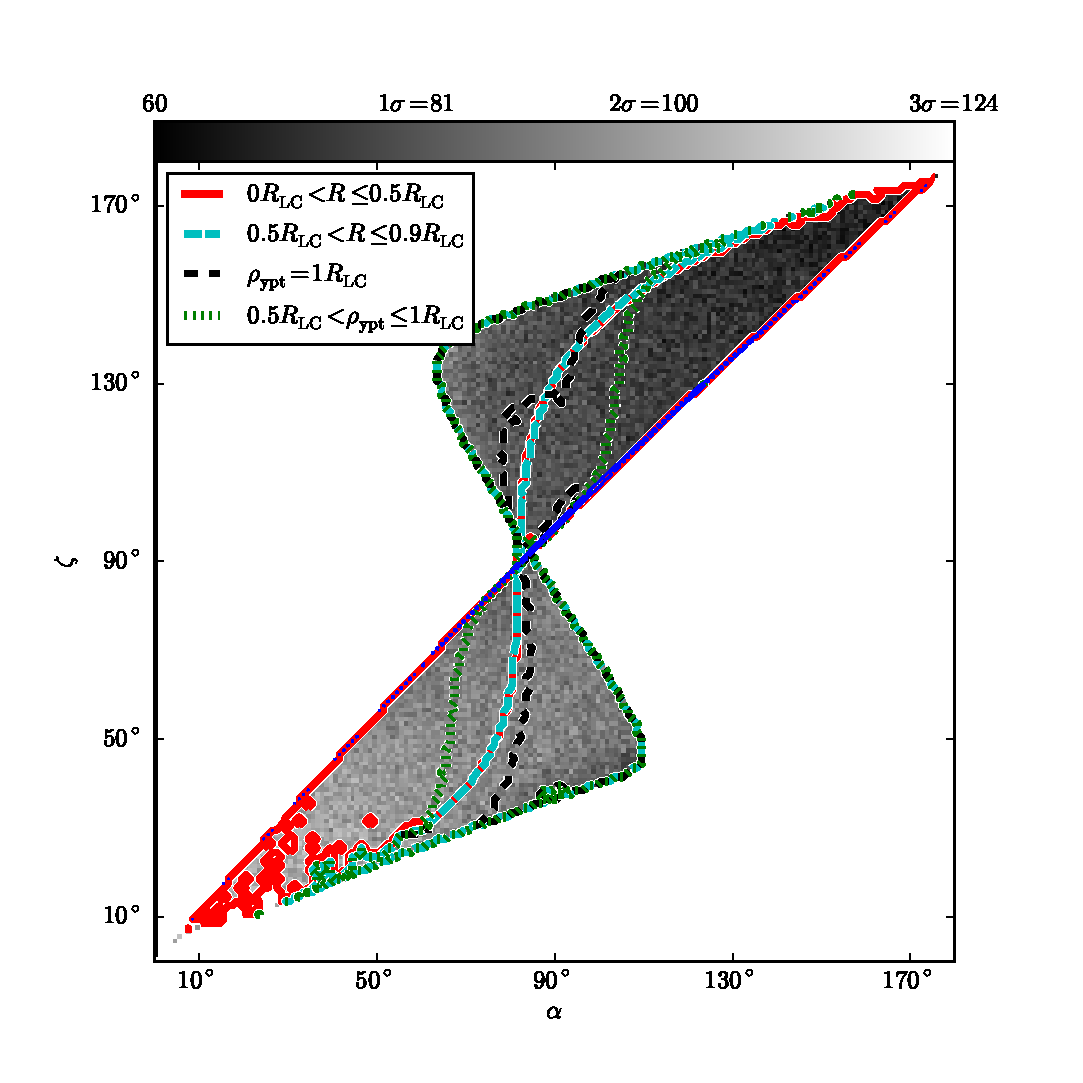
\includegraphics[width=0.98\textwidth]{chapters/pulsarAnatomy/figures/mapB1702allForward.eps}
%\caption{
%\label{}
%}
%\end{center}
%\end{figure}

\begin{figure}[htbp]
\vskip .85\textheight
\special{psfile=chapters/pulsarAnatomy/figures/pulsarAnatomy.eps hoffset=-5 voffset=-10 vscale=65 hscale=65}
\begin{center}
\caption[
Figure of the pulsar anatomy]{Figure of the pulsar anatomy. In Section \ref{sec:originAndSNR} we discuss the supernova remnant and
in Section \ref{sec:PWN} we discuss the pulsar wind nebula.  In Section \ref{sec:pulsarMag}
we explore the basics of the pulsar magnetosphere and review the two acceleration gap locations.
We also briefly summarize the neutron star interior in Section \ref{sec:NSandEOS}.
\label{fig:anatomy}
}
\end{center}
\vskip -0.2truecm
\end{figure}

\section{The Origin of Pulsars and Supernova Remnants}
\label{sec:originAndSNR}
A star will eventually collapse under its own gravity once it has exhausted its energy source.
If the star is massive enough, such a transition will come about violently in a
supernova explosion where most of the mass is expelled in a shell around the position
the star once was. This glowing mass is known as a supernova remnant which
we can continue to observe for 100 to 1000 years after the initial explosion.  The remainder of the
star collapses further either into a black hole or a neutron star depending on the
original mass of the star.  Since most of the angular momentum is conserved, the
much smaller, denser neutron star has a very small rotational period.
Additionally, magnetic flux is also conserved resulting in large magnetic fields.

For a normal star, the radius $R_0$ is $10^5$ to $10^8$ km and
the rotational period $P_0$ is a month to several years.
Equations for conservation of angular momentum and magnetic flux are
\begin{equation}
M R^2_0 \Omega_0=M R^2 \Omega
\end{equation}
\begin{center}
and
\end{center}
\begin{equation}
R^2_0 B_0 = R^2 B.
\end{equation}
With some physical considerations
(e.g. a very small period would result
in the star falling apart) it follows that
\begin{equation}
P \sim (R/R_0)^2 P_0 \sim .001 - 1 \quad \rm{seconds}\\\\
\end{equation}
\begin{center}
and
\end{center}
\begin{equation}
B \sim (R_0/R)^2 B_0 \sim 10^{10}-10^{12} \quad \rm{Gauss}.
\end{equation}

The rotational period of pulsars range from a couple of milliseconds to
several seconds.  For instance, PSR J$1748-2446$ad has one of the shortest
 periods known at $1.395$ ms \citep{hessels2006radio}.
The magnetic fields of pulsars are around $10^{10}$ to $10^{12}$ Gauss.
Magnetars, neutron stars with extremely strong magnetic fields, are said to have
magnetic fields of up to $10^{15}$ Gauss.  (The magnetic field of the Earth is
around $\sim 0.4$ Gauss and the magnetic field of the sun is around $\sim 1$ Gauss, for reference.)

One of the most massive pulsars is PSR J$1311-3430$ which has a mass
of $2.15$ to $2.7M_{\odot}$ (solar mass) from spectroscopic measurements \citep{romani2012psr}.
But the radius of neutron stars are tiny compared to solar radius at around $1.4\times10^{-5} R_{\odot}=10$km.
(The circumference is approximately the distance from
San Fransisco to San Jose.)

Neutron stars were first predicted as a result of
supernovae by \cite{baade1934super} many years before they
were observed.
Although the first supernovae was observed thousands of years ago,
the first pulsations (in radio) from pulsars were not observed 
(or more accurately, \textit{recognized}) until
relatively recently in 1967 to 1968.
The first correct and complete explanation of pulsars and their
connection to neutron stars followed rapidly by Gold and Pacini
\citep{pacini1967energy, gold1968rotating, pacini1968rotating}.
Today, the number of radio detected pulsars is in the low thousands and the number of energetic $\gamma$-ray
detected pulsars is in the low hundreds.
The number of galactic neutron stars is estimated at $\sim10^9$ although
how many are actually visible from Earth depends on a number of caveats \citep{colpi1998elusiveness}.




\section{Pulsar Wind Nebula}
\label{sec:PWN}

Unlike supernova remnants,
the pulsar wind nebulae are continuously renewed in energy
and are visible for much longer than supernova remnants.

Energy from the pulsar rotation is dissipated into the pulsar wind.
This dissipated spin down energy is given as
\begin{equation}
\dot{E}=I \Omega \dot{\Omega}
\end{equation}
where $I$ is the moment of inertia of the spinning neutron star and $\Omega$
is the angular frequency of the rotation.

The angular frequency and change in the angular frequency are
assumed to be related to each other as
\begin{equation}\label{eq:angFreq}\dot{\Omega} \propto \Omega^n\end{equation}
where $n$ is the braking index.
Using this relationship, one can solve for the age of the pulsar.

\begin{figure}[t!!]
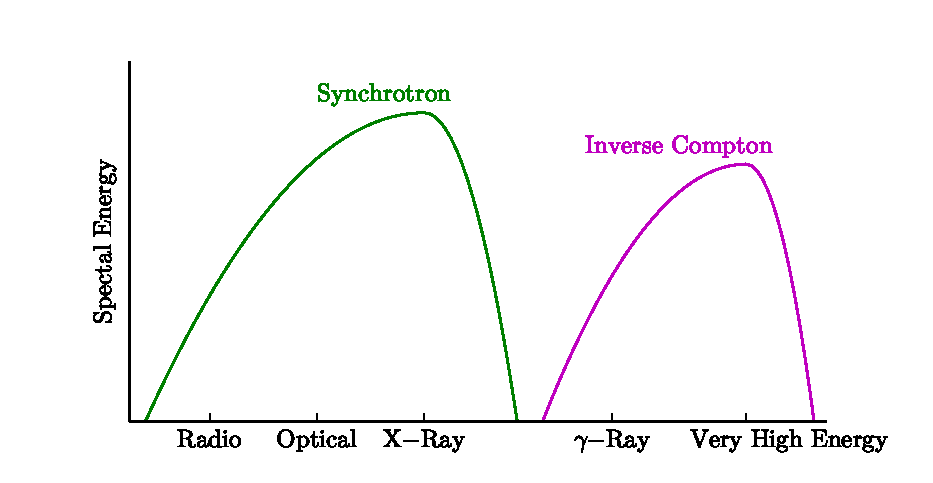
\includegraphics[width=.95\textwidth]{chapters/pulsarAnatomy/figures/spec.eps}
\caption[Typical pulsar wind nebula energy spectrum]{
\label{spec} Typical pulsar wind nebula energy spectrum.
Inspired by Figure 1.1 of \cite{vanEttenPhd2012}.}
\end{figure}

Interaction of this outflow with surrounding medium creates emission.
Particles interact with magnetic fields and photons to produce
synchrotron (very relativistic and ultra-relativistic electrons
gyrating in a magnetic field)
and inverse Compton (scattering of low energy photons
to high energy by ultra-relativistic electrons) emission. For
younger pulsars, this medium includes the cold supernova ejecta
beyond the termination shock.
Termination shock forms where the ram pressure of the wind 
balances the pressure of the surrounding medium.  
Figure~\ref{spec} shows a typical energy spectrum of a pulsar
wind nebula.


Of particular interests to polarization and geometric modeling
(the main theme of this thesis)
is the X-ray torus of pulsar wind nebulas which is further discussed
in Section \ref{subsec:ToriModeling}.
For more detailed overview of pulsar wind nebula see \cite{vanEttenPhd2012}
and
\cite{gaensler2006evolution}.

\section{Pulsar Magnetosphere}
\label{sec:pulsarMag}
The simplest model of the pulsar magnetosphere is
a very large magnetic (static) dipole in space.  Many of 
the well-used analytic formulations for analysis of pulsar
data are based on this simplistic assumption. 
We will discuss some of the models in later chapters.

The magnetic field of a \textit{rotating} vacuum dipole are given as

\begin{equation}
\label{eq:magField}
\vec{B}=-\frac{ \vec{m}(t_{\rm r}) +r\dot{\vec{m}}(t_{\rm r}) + r^2\ddot{\vec{m}}(t_{\rm r})}{r^3} + \left[ \frac{ 3\vec{m}(t_{\rm r}) +3r\dot{\vec{m}}(t_{\rm r}) + r^2\ddot{\vec{m}}(t_{\rm r})}{r^3} \cdot \mathbf{\hat{r}} \right] \hat{r}
\end{equation}
with
$\vec{m}(t_{\rm r})=m\left[\sin{(\alpha)} \cos{(t_{\rm r} \omega)} \hat{x}+ \sin{(\alpha)} \sin{(t_{\rm r} \omega)} \hat{y} +\cos{(\alpha)} \hat{z}\right]$
\citep{kaburaki1980determination}.
Here retarded time is $t_{\rm r}=t-r/c$
and $m$ is dipole magnetic moment.
This magnetic field contains information about relativistic effects
as well as a sweep-back form from the spin of the neutron star, making
it much more realistic than the classical dipole.  Conversely, it is much more difficult
to use in analytical closed-form formulations without approximations.
We use this form of the magnetic field extensively in modeling
of both the radio and $\gamma$-ray emission in our computational 
models.

In the pulsar magnetosphere, two primary regions emit photons: the polar gap
and the outer gap.  The polar gap is located near the magnetic pole of the pulsar
and relatively low in the magnetosphere near the surface of the neutron star.
Here the magnetic field is the strongest.   Emission is produced by curvature 
radiation.  Further, interaction of photons within the strong magnetic field
produce electron-position pair that then cause a cascade effect.  The
polar gap is the classical location of radio emission.

The outer gap is located further out in the magnetosphere in comparison to 
the polar gap and is also in a wider range of altitudes as it is said
to follow particular field lines.  The existence of the outer gap
is based on the Goldreich-Julian density: 
\begin{equation}\rho=\frac{\vec{\nabla}\cdot \vec{E}}{4\pi}=-\frac{\vec{\Omega}\cdot \vec{B}}{2\pi}.\end{equation}
The Goldreich-Julian density is formulated from Gauss' Law applied
to a force free model:
\begin{equation}\vec{F}=\vec{E}+(\vec{\Omega}\times \vec{r})\times \vec{B}/c=0.\end{equation}
This density arises from the spin of the neutron star 
(a spherical electric conductor) in  
its own magnetic field. Such spinning causes a \textit{nonzero}
force but free charges from the neutron star rearrange
according to the Goldreich-Julian density
to cancel this rotation-induced electromotive force.

The outer gap is located on the outer side of the null charge surface,
a cone-like surface originating from the polar cap (and within
the region of open field lines).  
The open field lines are those that extend beyond the pulsar light cylinder
never to return to the other magnetic pole.
The light cylinder radius, $R_{\rm{LC}}$, is the distance from the
center of the neutron star at which co-rotating particles would be traveling at the
speed of light.
The null charge surface
is located at $\vec{B}\cdot\vec{\Omega}=0$ in the magnetosphere.  This surface
is then defined by the location of the curvature of the magnetic 
field lines changing direction in relation to the spin axis but is
also the location where $\rho=0$.  One side of the surface is of one charge
and the other side of the surface is of the opposite charge.  

Further, if the charged particles are located in the region of open 
field lines, the charged particles are not simply locked in the
magnetosphere but can escape along the open field lines out of the 
magnetoshere and into space.  This exodus of charged particles is
favorable near the null charge surface because of the proximity 
of charged particles of opposite sign.  

This outflow creates a gap in the charge density (the outer gap)
where free charges can accelerate to relativistic energies and
emit in the $\gamma$-rays.  Further, this charge-starved
region is the location of cascade processes of pair-production. 

Charged particles in the magnetosphere are argued to co-rotate 
with field lines while traveling along the field lines.
In particular, we can note that gyrating motion of the 
particles around field lines will dissipate quickly through
synchrotron radiation.  
Synchrotron lifetime of electron is $T_{\rm s}=(5.1\times10^8 /B^2)\sqrt{1-v^2/c^2} $ s,
where $B$ is in Gauss
\citep{lyne2006pulsar}.
This timescale is much smaller than
the travel time of a particle following a field line thus
any gyration will be dissipated.

A third gap has been argued to exist that bridges the outer gap region
and the polar cap gap and is called the slot gap.  
This gap is thin and extends from the polar cap to the light cylinder following
the last closed field lines.
The $\gamma$-ray model with emission from
this gap is called the two-pole caustic model \citep{dyks2003two}. 
This model will be mentioned again in Chapter \ref{chapter:collaborationWork} 
in the work of $\gamma$-ray modeling in connection to polarization modeling.

\section{Neutron Star and Equation of State}
\label{sec:NSandEOS}
The surface of the neutron star is a rigid crystalline 
surface of iron nuclei.  With increasing depth this
lattice crust is made up of increasingly heavy nuclei.  
For a sufficiently large depth, free electrons 
penetrate the lattice.  At further depths, neutrons
are free in the lattice in the ``neutron drip'' region
\citep{kraus1986radio}.

Beyond this crust is an outer core made of 
neutron super-fluid and proton superconductor.
The material is around $95\%$ neutrons.
During rotation, the crust and the core 
can decoupled due to slippage, causing star quakes.
The quakes are seen as glitches in the pulsar phase data.

The neutron star interior is made up of ultra-dense nuclear material
beyond any known substance obtainable in a laboratory.  Neutron
stars are therefore valuable probes of the fundamental nature of 
matter.  Numerous theoretical equations of state for the stellar
core exist in the literature
although only one can be the correct and 
true equation.  Accurate measurements of neutron stars with 
extreme mass are often used to rule out several of these formulations.
The exact composition of this inner core is still
an area of active research (see e.g. for overviews \citealp{becker2009neutron}).

\section{Pulsar Populations and Age}
\label{sec:popAndAge}

\begin{figure}[t!!]
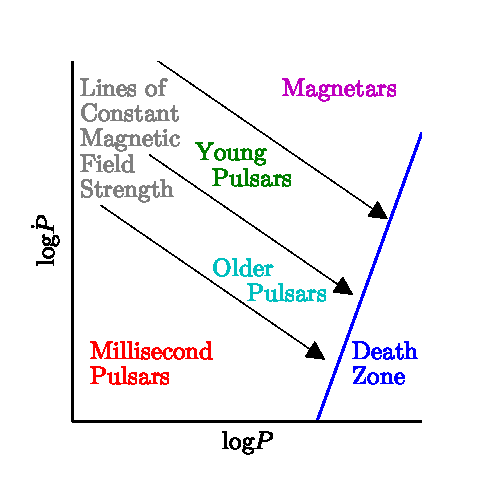
\includegraphics[width=.95\textwidth]{chapters/pulsarAnatomy/figures/ppdot.eps}
\caption[Period-period derivative schematic plot]{
\label{fig:ppdot} Period-period derivative schematic plot.}
\end{figure}

As pulsars age, their rotational period slows due to 
the loss of energy into the pulsar wind. 
Integration of Equation \ref{eq:angFreq} gives the characteristic
age of the pulsar as $t=P/2\dot{P}$
where $n=3$ or equivalently, $P\dot{P}$ is the
constant that relates $\Omega$ and $\dot{\Omega}$.
This relation is based on the assumption 
that the magnetic field
remains constant over time.

Figure~\ref{fig:ppdot} shows a schematic of various
pulsar populations.  Most pulsars start their
life in the upper left corner of the $P$--$\dot{P}$ diagram
and move diagonally downward along lines of constant
magnetic field strength.  Eventually, pulsars enter the ``death zone'' 
where they are not energetic enough to be observed.

In this thesis work, we focus on young pulsars
that are energetic enough to emit in both
radio and $\gamma$-ray wavelengths, allowing
for possible multi-wavelength studies.
Another population of pulsars that 
are energetic enough to emit in the
$\gamma$-rays are the millisecond pulsars
located in lower left corner of Figure~\ref{fig:ppdot}.

While young pulsars are rotation-powered, rotating
through the loss of rotational energy, millisecond
pulsars are accretion powered.  They are ``spun up''
by their companion star.
When the companion star of the neutron star overflows
the Roche lobe, it imparts material and angular momentum
onto the pulsar.  As a result, millisecond pulsar
periods are much faster and more 
precise compared to normal pulsar periods.











\chapter[Introduction: Radio and Pulsars]{Introduction to Radio Wavelength Emission Physics and Modeling of Pulsar Magnetospheres}
\label{chapter:radioAndPulsars}
In this chapter we will explore in more depth the physical models of the pulsar magnetosphere and 
physical phenomena highly relevant to fully understanding
the observed emission.  The focus here is
on analytic models derived elsewhere and 
standard to the current understanding
of pulsar magnetospheres.  
We will discuss further the numerical models of pulsars
utilized in this thesis in Chapter \ref{chapter:numericalModels}. 

\section{Polarization}
\label{sec:polarization}

William Hilter and John Hall first observed polarization of starlight in 1949 \citep{hiltner1949polarization,hall1949observations}.
Polarization was soon linked to magnetic fields of the galaxy 
by Leverrett Davis, Jr. and Jesse Greenstein \citep{davis1951polarization}.

Pulsars have strong magnetic fields which gives rise to not only their 
extremely focused beam of emission but also coherent light with 
defined polarization.  
Polarization is a means of observing the magnetic field lines of these incredibly small,
far away objects.  That we can make such a bold measurement speaks to the extremes of the
pulsar.


Polarization is most often reported in terms of Stokes parameters, $I$, $Q$, $U$, and $V$.
Stokes parameters are a standard way of representing polarization.
At a radio telescope with polarization measurement capabilities, the incoming
electromagnetic wave is converted to electric voltage in two independent
feeds.  Linear feeds will measure polarization aligned along $x$ and $y$ Cartesian coordinates
while circular feeds will measure polarization as right-handed or left-handed.

Components of the linear and circular feeds can be converted to Stokes parameters
\begin{equation}
 \begin{array}{lcl}
    I=\langle E_{\rm X}^{2} \rangle + \langle E_{\rm Y}^{2} \rangle &\textrm{and}& I=\langle E_{\rm R}^{2} \rangle + \langle E_{\rm L}^{2} \rangle,\\
    Q=\langle E_{\rm X}^{2} \rangle - \langle E_{\rm Y}^{2} \rangle &\textrm{and}& Q=2\langle E_{\rm R}^{2} E_{\rm L}^{2} \cos {\left(\kappa_{\rm RL}\right)} \rangle,\\
    U=2\langle E_{\rm R}^{2} E_{\rm L}^{2} \cos {\left(\kappa_{\rm XY}\right)} \rangle &\textrm{and}& U=2\langle E_{\rm R}^{2} E_{\rm L}^{2} \sin {\left(\kappa_{\rm RL}\right)} \rangle,\\
    V=2\langle E_{\rm R}^{2} E_{\rm L}^{2} \sin {\left(\kappa_{\rm XY}\right)} \rangle &\textrm{and}& V=\langle E_{\rm R}^{2} \rangle - \langle E_{\rm L}^{2} \rangle,
  \end{array}
\end{equation}
where $\kappa_{\rm AB}$ is the phase difference.
With a little manipulation, we can see that $I^2=Q^2+U^2+V^2$ if the incoming signal is
totally polarized.  Typically, $(Ip)^2=Q^2+U^2+V^2$, where $p$ is the degree of polarization.

\begin{figure}[h]
\vskip .42\textheight
\begin{center}
%\includegraphics[width=.7\textwidth]{chapter2figures/totDirFitPhi.eps}
\special{psfile=chapters/radioDataAnalyticModels/figures/stokesFigure.eps hoffset=-100 voffset=-300 vscale=100 hscale=100}
\caption[Visualization of Stokes parameters]{
Visualization of Stokes parameters.  The absolute value of linear polarization ($|L|=\sqrt{U^2+Q^2}$ )
occupies the $U$-$Q$ plane while circular polarization $V$ is the third Cartesian axis.  The
total polarized intensity is labeled $pI$ and the total intensity which extends beyond
the polarized intensity is labeled $I$.
}
\label{fig:stokes}
\end{center}
\vskip -.03\textheight
\end{figure}

Stokes parameters are a convenient way of expressing polarization and is particularly useful for
describing partially polarized light using $p$. The Stokes parameters occupy the so-called
Poincar\'{e} sphere of optics where $Q$, $U$, and $V$ are the axes and $pI$ is the radius of the
sphere (Figure~\ref{fig:stokes}).  The polarization angle ($\psi$) and linear polarization ($L$) relate to the polar coordinates of
$Q$ and $U$:

\begin{equation}
    |L|=\sqrt{U^2+Q^2}
\end{equation}
\begin{center}
and
\end{center}
\begin{equation}
    \psi=\frac{1}{2} \arctan{\left(\frac{U}{Q}\right)}.
\end{equation}

Polarization data that we received from collaborators is in the form
of $Q$, $U$, $V$, $I$ versus pulsar rotation period phase and we
calculate polarization using $Q$ and $U$.

Further error bars for the polarization are calculated using the
following formula (standard error propagation):

\begin{equation}\sigma_{\psi}(\phi)=\frac{1}{2} \frac{\sqrt{\langle\sigma_{U{\rm off}}*Q(\phi)\rangle^2+\langle\sigma_{Q{\rm off}}*U(\phi)\rangle^2}}{\langle Q(\phi)\rangle^2+\langle U(\phi)\rangle^2}.\end{equation}

The values $\sigma_{Q{\rm off}}$ and $\sigma_{U{\rm off}}$ are the standard deviation in the off-pulse phases of $Q$ and $U$.
Note that $Q$, $U$, and $\sigma_{\psi}$ are all functions of the 
pulsar rotation period phase, $\phi$.


\section{Effects of Interstellar Medium} \label{sec:interstellarScattering}
The space between us and pulsars is not empty but is full
of ionized medium that effects electromagnetic waves.
Such medium modifies the signal in several ways which we can
quantify.

The dispersion measure is the total density of free electrons ($N(l)$) over the intervening space that the signal from the pulsar
travels:
\begin{equation} DM=\int_0^L N(l) \mathrm{d}l. \end{equation}

The dispersion measure is related to the frequency of the emission ($\nu$) and the time delay of the emission ($t$):

\begin{equation}DM_{[\textrm{cm}^{-3}\textrm{pc}]}=2.410\times10^{-4} \textrm{ } t_{[\textrm{s}]}\textrm{ } \nu^2_{[\textrm{MHz}]}.\end{equation}

This formula is useful for calculating the expected time delay between frequencies:

\begin{equation}
\Delta t_{[\textrm{s}]}= \frac{DM_{[\textrm{cm}^{-3}\textrm{pc}]}}{2.410\times 10^{-4}} \left\{  \frac{1}{\nu^2_{2 [\textrm{MHz}]}} - \frac{1}{\nu^2_{1 \lbrack\textrm{MHz}\rbrack}}  \right\}.\end{equation}

In particular, we wished to quantify the time delay in PSR J1420$-$6048 because the fit was simultaneous
in two frequencies, 10cm and 20cm (Section \ref{sec:J1420}).  
In the end, we found that any time delay due to dispersion
was overpowered by our uncertainty in phase. (See \cite{rohlfs2000tools} for a particularly well formulated
presentation of the dispersion measurement calculation.)

Another effect of interstellar medium on measurements is interstellar scattering.
The scattering of emission in the medium results in multipath propagation.  
The effects of interstellar scattering manifest themselves in pulsar data as
a broadening of the trailing end of the intensity pulse and a flattening of the polarization data versus
phase.

This scattering effect is mathematically described as a convolution of the unscattered
Stokes parameters with a scattering kernel:

\begin{equation}
\begin{array}{l}
I^{\rm scat}=\int I(\phi(t')) g(t-t') dt,\\
Q^{\rm scat}=\int Q(\phi(t')) g(t-t') dt,\\
U^{\rm scat}=\int U(\phi(t')) g(t-t') dt,\\
V^{\rm scat}=\int V(\phi(t')) g(t-t') dt.
\end{array}
\end{equation}
This relation is used for model $Q$ and $U$
in Chapter \ref{chapter:tacklingPolarization}.

Analytical scattering kernels exist assuming various distributions
of interstellar medium.  
The scattering kernel assuming a thin scattering screen 
halfway between source and observer is given by 

\begin{equation}\label{eq:gts2}
g_{ts}(t-t')=\left\{
\begin{array}{lr}
0,                       & t-t' < 0 \\
e^{-(t-t') / \tau_{\rm s}},  & t-t' > 0
\end{array}
\right.
\end{equation}
\citep{williamson1972pulse,williamson1973pulse}.
The scattering kernel assuming a thick screen near the
source is given by 
\begin{equation}
g_{\rm ths}(t-t')=\left\{
\begin{array}{lr}
0,                       & t-t' < 0 \\
\sqrt{\frac{\pi \tau_{\rm s}}{4t^3}} e^{-\pi^2\tau_{\rm s}/16t},  & t-t' > 0.
\end{array}
\right.
\end{equation}
The scattering kernel assuming uniform medium is given by
\begin{equation}
g_{\rm um}(t-t')=\left\{
\begin{array}{lr}
0,                       & t-t' < 0 \\
\sqrt{\frac{\pi^5 \tau_{\rm s}^3}{8t^5}} e^{-\pi^2\tau_{\rm s}/4t},  & t-t' > 0.
\end{array}
\right.
\end{equation}
The variable $\tau_{\rm s}$ is a characteristic scattering time.
The simplest kernel $g_{\rm ts}$ is used in Chapter \ref{chapter:tacklingPolarization}  in 
modeling scattering.

Finally, pulsar polarization data is Faraday rotated
by interstellar medium.  Faraday rotation is a powerful
tool for probing interstellar scattering but for us it is 
a nuisance to be removed from the data.  The degree of Faraday rotation
is related to frequency and can be removed by comparing data
from multiple frequencies.  Considering that $\Delta\psi$ is often
treated as a nuisance parameter, the accuracy of this removal
is not very important.  



\section{Beaming Geometry}
\label{sec:beamingGeometry}
Assuming a beam of emission centered on the 
magnetic axis, the
relationship between pulse width
in phase and the opening angle of the
cone structure where emission originates
can be derived in closed form.
The cone is centered on the magnetic 
axis defined by 

\begin{equation}
\label{equ:m}
\hat{m}=\cos{(\phi)} \sin{(\alpha)} \hat{x} + \sin{(\phi)} \sin{(\alpha)} \hat{y} + \cos{(\alpha)} \hat{z}
\end{equation}
where $\phi$ is the phase of the pulsar
as it rotates about $\hat{\Omega}=\hat{z}$.
The pulse width is $W$ and thus
for a symmetric cone, the 
pulse is seen between $\phi=-W/2$ and $\phi=W/2$
in phase.
The angle between $\hat{m}$ and the
line of sight at the maximums ($\phi=-W/2$ and $\phi=W/2$) will also be the opening
angle.  The line of sight is given by 
\begin{equation}
\hat{n}=\sin{\zeta} \hat{x}+\cos{\zeta} \hat{z}
\end{equation}
and the relation between opening angle and 
pulse width is
\begin{equation}
\label{equ:ndotm}
\hat{n}\cdot\hat{m}=\cos{\Gamma}=\sin{\zeta} \cos{W/2} \sin{\alpha} + \cos{\zeta} \cos{\alpha} 
.\end{equation}
This equation makes no assumptions about the form of the magnetic field lines.
The angle $\alpha$ is between the spin axis and the magnetic axis and the
angle $\zeta$ is between the spin axis and the line of sight.

We can further relate the pulse width to emission height for a
dipole magnetic field.  The last closed field lines
which define the emission cone for a simple dipole
have the form 
\begin{equation}
\label{equ:dipole}
\mathbf{r}=\sin^3\theta \hat{x} + \sin^2\theta \cos{\theta} \hat{z}
\end{equation}
\begin{center}
and
\end{center}
\begin{equation}
R=|\mathbf{r}|=\sin^2\theta
\end{equation}
in polar coordinates where $R$ is the emission 
altitude measured in $R_{\rm LC}$, light cylinder
radius.
In this coordinate system, $\hat{m}=\hat{z}$.

The angle $\Gamma$ between $\hat{n}$ and $\hat{m}$
will be approximately the angle between 
\begin{equation}
\hat{T}=\frac{d\mathbf{r}/d\theta}{|d\mathbf{r}/d\theta|}
\end{equation}
(the curvature of $\mathbf{r}$) and $\hat{m}$.
This is actually a far field approximation 
but is appropriate because 
the observer is very far from the pulsar.

We can then relate the opening
angle to the altitude using Equation \ref{equ:dipole}.
Again using $\hat{m}=\hat{z}$, Equation \ref{equ:dipole} and Equation \ref{equ:m}:
\begin{equation}\hat{T}\cdot\hat{m}=\frac{2-3\sin^2\theta}{\sqrt{4-3\sin^2\theta}}.\end{equation}

Using $R=\sin^2\theta$ and approximating $R$ as small, 
\begin{equation}\hat{T}\cdot\hat{m}=1-9R/8.\end{equation}

Further using $\hat{T}\cdot\hat{m}\approx\cos{\Gamma}\approx 1-\Gamma^2/2$ and Equation \ref{equ:ndotm},
we get:
\begin{equation}
R=\frac{4}{9}\arccos^2\left[\sin{\zeta}\cos{\frac{W}{2}}\sin{\alpha}+\cos{\zeta}\cos{\alpha}\right]
.
\end{equation}

This equation then relates the width of the intensity pulse to the altitude of
emission.

\section{Rotating Vector Model}
\label{sec:RVMformula}

The rotating vector model (RVM) relates the 
geometrical angles $\alpha$ (the angle between
the spin axis and the magnetic axis) and $\zeta$ (the
angle between the spin axis and the line of sight)
to the polarization position angle $\psi$ for 
a given phase angle $\phi$.

We start with a fixed magnetic axis given by
\begin{equation}
\hat{m}=\sin{\alpha}\hat{x}+\cos{\alpha}\hat{z}
\end{equation}
and a viewing direction given by
\begin{equation}
\hat{n}=\sin{\zeta}\cos{\phi}\hat{x}+\sin{\zeta}\sin{\phi}\hat{y}+\cos{\zeta}\hat{z}.
\end{equation}
The polarization angle with respect to $\hat{z}=\vec{\Omega}$
is the difference in angle between the projection of $\hat{z}$
onto the viewing plain and the projection of the vector 
$\hat{n}-\hat{m}/|\hat{n}-\hat{m}|$.
The viewing plane is defined as orthogonal to $\hat{n}$.
These projections can then be given by the vector rejections:
\begin{equation}
\mathbf{P}_{\Omega}=\mathbf{\hat{z}}-(\mathbf{\hat{z}}\cdot\mathbf{\hat{n}})\mathbf{\hat{n}}
\end{equation}
and 
\begin{equation}
\mathbf{P}_{m-n}=\frac{\hat{n}-\hat{m}}{|\hat{n}-\hat{m}|}-\left(\frac{\hat{n}-\hat{m}}{|\hat{n}-\hat{m}|}\cdot\mathbf{\hat{n}}\right)\mathbf{\hat{n}}
.\end{equation}

The polarization angle can be calculated as
\begin{equation}
\tan{\psi}=\frac{|\mathbf{P}_{m-n}\times\mathbf{P}_{\Omega}|}{\mathbf{P}_{m-n}\cdot\mathbf{P}_{\Omega}}
.\end{equation}

Plugging in the above formulas and simplifying gives us the familiar 
rotating vector model equation:
\begin{equation}
\tan{\psi}=\frac{
-\sin{\alpha}\sin{\phi}
}{
\cos{\alpha}\sin{\zeta}-\cos{\phi}\cos{\zeta}\sin{\alpha}
}
.\end{equation}



\chapter{Numerical Models of Pulsar Magnetosphere}
\label{chapter:numericalModels}

This chapter focuses on numerically derived 
pulsar models.  We concentrate on the geometrically based 
modeling of pulsar magnetic field lines.  From this 
formulation, we derive the $\gamma$-ray light curves
and the radio polarization position angle sweeps.  
We also discuss
the X-ray pulsar wind tori model which is often used
in conjunction with the $\gamma$-ray and radio modeling.

\section{Magnetic Field Line Calculation}
\label{sec:calculation}
In this section we discuss how to calculate $\zeta$, the viewing angle, and $\phi$, the pulsar phase
from a photon at a given point in the magnetosphere of a pulsar
with $\alpha$, the angle between rotation axis and magnetic axis.
First we describe the magnetosphere in mathematical terms.
Next we calculate the velocity of a charged particle within
the magnetosphere which dictates the motion of the particle.  
Finally, we describe the projection of photons produced by curvature
radiation from the charged particles onto the field of view.
These photons are the observables from earth.

\subsection{A Point in the Magnetosphere}

In the frame where the magnetic axis is along the $z$ axis, $\theta_{B}(\phi_{B})$ defines
the polar cap edge. The polar cap is defined by the last closed field lines
on the surface of the pulsar.  Field lines originating from within the cap are open
and extend beyond the light cylinder never to return to the surface
of the pulsar.  The light cylinder is the region where co-rotating
particles are traveling at the speed of light.
The fractional distance from the cap edge is given by the parameter $w$,
where $w=1$ is the center of the cap at the magnetic pole and $w=0$ is the edge of the cap.
The angle from the magnetic axis is
$\theta_w=\theta_{B}(1-w)$.  A field line traced from the neutron 
star surface can be defined by a point using
the cap parameters:

\begin{equation}
\begin{array}{ccc}
x= & \sin(\theta_w) \cos(\phi_B), \\
y= & \sin(\theta_w) \sin(\phi_B), \\
z= & \cos(\theta_w). \end{array}
\end{equation}

This point is
in the frame where the magnetic axis is along $\hat{z}$.
This point in the frame where the axis
of rotation is along $\hat{z}$
is obtained by applying a rotation matrix as follows:

\begin{equation}
\begin{array}{c}
             \\
R_{y}(\alpha)\\
              \end{array} 
\qquad
\left( \begin{array}{c}
x  \\
y  \\
z  \end{array} \right)
\qquad
\begin{array}{c}
   \\
=  \\
   \end{array}
\qquad
\left[ \begin{array}{ccc}
\cos \alpha  & 0 & \sin \alpha  \\
0            & 1 & 0            \\
-\sin \alpha & 0 & \cos \alpha  \end{array} \right]
\qquad
\left( \begin{array}{c}
\sin \theta_w \cos \phi_B  \\
\sin \theta_w \sin \phi_B  \\
\cos \theta_w  \end{array} \right)
.\end{equation}

In the new coordinates the starting point of a given magnetic field line is given by:

\begin{equation}
\begin{array}{cc}
x= &  \cos\phi_B \sin\theta_w \cos\alpha + \cos\theta_w \sin\alpha, \\
y= &  \sin\phi_B \sin\theta_w, \\
z= & -\cos\phi_B \sin\theta_w \sin\alpha +  \cos\theta_w \cos\alpha. 
\end{array}
\end{equation}

This can be translated into the more useful spherical coordinates as follows:

\begin{equation}
\begin{array}{cc}
r=      & R_{\rm{NS}}, \\
\theta= & \arctan(\sqrt{(x^2+y^2)/z_w)}\textrm{ }), \\
\phi=   & \arctan(y/x). \\ 
\end{array} 
\end{equation}


\subsection{Velocity and Motion of a Charged Particle}

The velocity ($\vec{v}_{\rm tot}$)
of a charged particle within the magnetosphere 
can be calculated in order
to obtain the direction of travel.
We can calculate the magnetic field strength at this point $(r,\theta,\phi)$ using
Equation \ref{eq:magField}.  The field at this location points in the direction
$\hat{v}_B$.  Charged particles will travel in this direction along the magnetic
field. Additionally, the velocity due to co-rotation with the star is
given by $\vec{v}_{\rm t}=<-y,x,0>$.

We need the \textit{magnitude} of $\vec{v}_B$ to find
$\vec{v}_{\rm tot}=\vec{v}_B+\vec{v}_{\rm t}$;
only the direction is obtained by Equation \ref{eq:magField}.
We estimate $|\vec{v}_B+\vec{v}_{\rm t}|=c=1$ and manipulate
this to

\begin{equation}
\vec{v}_B^2+ 2 \vec{v}_B \cdot \vec{v_{\rm t}} + \vec{v_{\rm t}}^2 = 1.
\end{equation}
By simply expanding out, the equation becomes
\begin{equation}
v_B^2+(\vec{v}_{\rm t} \cdot \hat{v}_B)^2 + 2 \sqrt{v_B^2} \hat{v}_B \cdot \vec{v}_{\rm t} -(\vec{v}_{\rm t} \cdot \hat{v}_B)^2 + v_{\rm t}^2 = 1.
\end{equation}
The above equation can be further manipulated to
\begin{equation}
|\vec{v}_B|=-\vec{v}_{\rm t} \cdot \hat{v}_B + \sqrt{(\vec{v}_{\rm t} \cdot \hat{v}_B)^2 - v_{\rm t}^2 +1}
\end{equation}
thus solving for the magnitude of the velocity on a charged particle from the magnetic field
and $\vec{v}_{\rm tot}=\vec{v}_B+\vec{v}_{\rm t}$ is obtained.

Further, a charged particle moving along the field line will be located
after one time step at approximately:
\begin{equation}
  \begin{array}{c}
x'=x+|v_B|\frac{B_x}{\sqrt{B_x^2+B_y^2+B_z^2}} \Delta t, \\
y'=y+|v_B|\frac{B_y}{\sqrt{B_x^2+B_y^2+B_z^2}} \Delta t, \\
z'=z+|v_B|\frac{B_z}{\sqrt{B_x^2+B_y^2+B_z^2}} \Delta t .\end{array}
\end{equation}
ignoring higher order terms.
We set $\Delta t =1/2500$ for all calculations.

\subsection{Projection onto the $\zeta$--$\phi$ Viewing Plane}

The total velocity can be expressed in spherical coordinates, $(\phi_{\rm v},\theta_{\rm v})$.
This velocity of a charged particle in the magnetosphere is
in the same direction as the direction of a photon emitted tangent to the field line
at the given point.
In order to project this photon onto the plane of the sky, 
the viewing angle is simply given as $\zeta=\theta_{\rm v}$.

The phase at which the photon arrives at an observer is given as
$\phi=\phi_{\rm v} +\Delta\phi_{\rm{travel-time}}$.  The extra piece $\Delta\phi_{\rm{travel-time}}$
is needed because photons emitted at different locations in the magnetosphere
will arrive at the observer at different times even if they are aimed in the same direction.
This change in phase is known as the travel time correction.
The phase difference is related to the speed of light and the spin of the pulsar:
$\Delta\phi_{\rm{travel-time}}=\Omega \Delta t_{\rm{travel-time}}=\Omega \Delta d_{\rm{travel-time}}/c$.
The variable $\Delta d_{\rm{travel-time}}$ is then the distance along the line of sight 
to the observer which is $\Delta d_{\rm{travel-time}}=\vec{v}_{\rm tot} \cdot <x,y,z>$.  
Since $\Omega=1$ and $c=1$, the phase is simply given as
$\phi=\phi_{\rm v} + \vec{v}_{\rm tot} \cdot <x,y,z>$.



\section{Polarization Calculation}
\label{sec:numericalPolarization}

Following a particle along a field line is
important for tracking emission from a particular zone
on the cap usually expressed as a function of $w$,
the fractional distance between the magnetic
pole and the edge of the open-zone cap.
It is also important for calculating the
polarization position angle ($\psi$) of a photon emitted
at a given location.
The position angle is the angle between the spin
axis and the acceleration vector projected onto viewing plane.
In order to calculate the position angle of the emission,
the acceleration of the 
particle which emitted the curvature radiation must be calculated.
We must calculate the properties of the charged particle
one time step forward.

After a time step, the new magnetic 
field at the new location is $\vec{B'}$ (calculated from Equation \ref{eq:magField}).
But in the mean time, our reference frame (the pulsar) has rotated by $\Delta \theta$.
$\Omega=\Delta \theta / \Delta t = 1$ so $\Delta \theta = 1/25000$
Because of this rotation, the point is actually located at:

\begin{equation}
\left( \begin{array}{c}
x'' \\
y'' \\
z'' \end{array} \right)
\qquad
 \begin{array}{c}
  \\
= \\
  \end{array}
\qquad
\left( \begin{array}{ccc}
\cos\Delta\theta & -\sin\Delta\theta & 0 \\
\sin\Delta\theta &  \cos\Delta\theta & 0 \\
0                & 0                 & 1 \end{array} \right)
\qquad
\left( \begin{array}{c}
x' \\
y' \\
z' \end{array} \right)
\qquad
 \begin{array}{c}
  \\
= \\
  \end{array}\end{equation}
\begin{equation}
\qquad
\left( \begin{array}{c}
x'\cos\Delta\theta - y'\sin\Delta\theta \\
x'\sin\Delta\theta - y'\cos\Delta\theta \\
z' \end{array} \right). \end{equation}

Also the magnetic field is now

\begin{equation}
\begin{array}{c}
             \\
\vec{B''}= \\
             \end{array}
\qquad
\left( \begin{array}{ccc}
\cos\Delta\theta & -\sin\Delta\theta & 0 \\
\sin\Delta\theta &  \cos\Delta\theta & 0 \\
0                & 0                 & 1 \end{array} \right)
\qquad
\begin{array}{c}
             \\ 
\vec{B'} \\
             \end{array}. \end{equation}

Again, the co-rotation velocity is $\vec{v}_{\rm t}''=<-y'',x'',0>$ and
the magnitude of the velocity from the magnetic field at this new location is
\begin{equation}
|\vec{v}_B''|=-\vec{v}_{\rm t}'' \cdot \hat{v}_B'' + \sqrt{(\vec{v}_B'' \cdot \hat{v}_B'')^2 - v_{\rm t}''^2 +1}
.\end{equation}
As before, we can calculate the total velocity; using this and the previous
velocity, we can calculate the acceleration of a particle. 
The change in the velocity is given by  $\Delta t \vec{a} = \vec{v}_{\rm tot}'' - \vec{v}_{\rm tot}$.

As stated earlier, the position angle is the angle between the spin axis and the acceleration vector projected onto a viewing
plane.
The projection of the acceleration vector onto the 
viewing plane in the direction of the velocity is given as 
the vector rejection of $\vec{a}$ in direction $<v_x,v_y,v_z>$.
The vector rejection is given as:
\begin{equation}\vec{p}_a=\vec{a} - (\vec{a} \cdot <v_x,v_y,v_z>) <v_x,v_y,v_z>.\end{equation}

Similarly, the project of $<0,0,1>$, the spin axis $\vec{\Omega}$, onto viewing plane is given as
\begin{equation}\vec{p}_{001}= <0,0,1> -(<0,0,1> \cdot <v_x,v_y,v_z>) <v_x,v_y,v_z> = <-v_z v_x,-v_z v_y,1-v_z v_z>.\end{equation}

The projection vectors are normalized and the angle between them simply gives the polarization position angle
of that photon:
\begin{equation}\psi=\arccos(||\vec{p}_a|| \cdot ||\vec{p}_{001}||).\end{equation}
Each position angle is a function of $\alpha$, $\zeta$, and $\phi$.  
If $\alpha$ and $\zeta$ are constant and $\psi$ is plotted versus $\phi$,
the result is the polarization sweep versus the pulsar phase.

\section{Numerical (Geometrically-Based) Modeling in Other Wavelengths}
\label{sec:ModelingOtherWavelengths}
Often in studies of pulsar polarization, data in other wavelengths is available
and can be used to cross-compare results obtained from modeling
of the position angle sweep.
In particular, X-ray data of the pulsar wind nebula can 
be used to derive the viewing angle $\zeta$ and
modeling of the $\gamma$-ray light curve derive independent
$\alpha$ and $\zeta$ parameters.  Here we will 
briefly describe these relevant models.

\subsection{Pulsar X-Ray Wind Tori Model} 
\label{subsec:ToriModeling}
The fitting of the pulsar wind tori model in the X-ray band is described in
detail in \cite{ng2004fitting} and this section is but a 
brief overview.  

The X-ray pulsar wind nebula is sometimes visible around
the central pulsar; the orientation of the pulsar and direction of
the spin axis can be 
quantified using the visible nebula.  
The boundary of the pulsar wind nebula is marked by
the location where the ram pressure of the outflowing material equals
the external pressure of the surrounding medium.
The radius of this termination shock boundary is
\begin{equation}
r_{\rm termination}\approx \left(\frac{\dot{E}}{4\pi c P_{\rm ext}} \right)^{1/2}
\end{equation}
where $\dot{E}$ is the spin down energy and $P_{\rm ext}$ is the
external pressure.
\cite{ng2004fitting} assumed simple equatorial
torus with a Gaussian intensity cross section profile
to describe the brightness of the nebula tori.
The fit parameters for this model are $\Psi$, the polar
axis at a position angle; $\zeta$, the viewing angle measured
from the rotation axis; $r$, the radial distance
to the brightest section of the circular tori; $\delta$,
a measure of the width of the circular tori; and $\beta$,
the bulk velocity of the post-shock flow.
Additionally, background must also be fit to 
the image and the point spread function needs to
be applied.

The apparent intensity is given as 
\begin{equation}
I \propto (1-\hat{n}\cdot \beta)^{-(1+\Gamma)} I_0
\end{equation}
\citep{pelling1987scanning}
where $\Gamma$ is the photon spectral index,
$I_0$ is the Synchrotron emission intensity and
$\hat{n}$ is the unit vector along the line of sight.
In terms of usable parameters:
\begin{equation}
I(x^\prime,y^\prime,z^\prime)= 
\frac{N}{(2\pi\delta)^2r} \times
\left(1 - \frac{y^\prime \sin \zeta}{\sqrt{{x^\prime}^2
+{y^\prime}^2}}\beta\right)^{-(1+\Gamma)}
e^{-\left[{z^\prime}^2+(\sqrt{{x^\prime}^2+{y^\prime}^2}-r)^2\right]/2\delta^2}
.\end{equation}
The parameters $x$ and $y$ are the coordinates of the CCD frame and $z$
is the line of sight.  The parameters $x^\prime$, $y^\prime$ and $z^\prime$
are the coordinates in the frame of the tori such that:
\begin{equation}
\begin{array}{ccc}
x^\prime&=&-x\cos \Psi -y\sin \Psi, \\
y^\prime&=&(x\sin \Psi - y\cos \Psi)\cos \zeta + z\sin \zeta, \\
z^\prime&=&-(x\sin \Psi - y\cos \Psi)\sin \zeta + z\cos \zeta.
\end{array}
\end{equation}
The photon spectral index is $\Gamma=1.5$.
For more details and caveats of the model and
fitting scheme, see \cite{ng2004fitting}. 

\subsection{Pulsar $\gamma$-Ray Light Curve Model}

In Section \ref{sec:calculation} we discussed the formulation
necessary to fire photons along magnetic field lines
of a rotating pulsar.  For modeling in the radio,
emission is assumed to come from a single set of magnetic
field lines at the same altitude. For modeling in the 
$\gamma$-rays, emission comes from the outer gap region
of the magnetosphere as discussed in Section \ref{sec:pulsarMag}.
Because emission comes from multiple altitudes, caustics, 
the enveloping of light-rays from multiple locations onto a 
single location, occur.  These caustics give rise to 
sharp peaks in intensity of the $\gamma$-rays. 

Similar to \cite{romani2010constraining}, when modeling
$\gamma$-ray light curves, we apply a path-length cut-off
to the magnetic field lines that are allowed to emit.
Only for $s<2s_{\rm{NC,min}}+\rho_{\rm{ypt}}$ measured 
from the center of the pulsar 
along the arching field line are photons illuminated at
full strength.  Here $s$ is the path length of the 
magnetic field line, $s_{\rm{NC,min}}$ is the minimum
path length of field lines at a given fraction of the polar cap,
and $\rho_{\rm ypt}$ is the effective light cylinder radius.
Beyond which, illumination is damped according
to
\begin{equation}
e^{-[(s-2s_{\rm{NC,min}}-\rho_{\rm{ypt}})/\sigma_s]^2}. 
\end{equation}

This cut-off eliminates field lines that arch over the
pulsar and cross the null-charge surface far from the 
star.  These field lines create a secondary gap disjointed
from the main gap on the other side of the spin axis that
arguably does not exist in most pulsars from a phenomenological
stand point; an exception to this argument is the 
emission from the Crab pulsar \citep{moffett1996multifrequency}.

We must also prescribe radiating zones within the outer gap
and intensity weightings dependent on the location of the radiating
zones.  Typically, only field line at a certain $w$, the fractional distance
from the cap boundary, are considered to emit.  
The heuristic efficiency law 
\begin{equation}
w_0=\sqrt{10^{-33}\rm{erg s^{-1}}/\dot{E}}
\end{equation}
provides an estimation for the choice of $w$.
Theoretical basis for this model is provided in \cite{arons2006theory}
and observational evidence for this model is
provided in \cite{psrcat}.
A Gaussian spread is applied to the sheet defined
by $w_0$ in the magnetosphere to soften the
caustics seen in emission from a single $w$.

The figure of merit $\chi_3$ defined in
\cite{romani2010constraining} is often used for analyzing $\gamma$-ray light
curve data.  This minimization formula is given as
\begin{equation}
\chi_3\propto\sum_i\frac{(M_i-O_i)^2}{O_i} e^{-i/3}
\end{equation}
where $i$ is an index with the value $|M_i-O_i|$ sorted from largest
to smallest.  Here $M_i$ is the model data point
and $O_i$ is the observed data point.  Such a scheme will 
cause models that better match the intensity peaks in the light
curve to be favored during minimization of the function.
  




\chapter[Phenomenological Altitude Limits of RVM]{Phenomenological Altitude Limits of Rotating Vector Model Fitting}
\label{chapter:phenomenologicalFitting}

\paperref{This section is based on work done for
``Altitude Limits for Rotating Vector Model Fitting of Pulsar Polarization''
\citep{craig2012altitude}}

Traditional pulsar polarization sweep analysis starts from the point dipole rotating vector model
(RVM) approximation. If augmented by a measurement of the sweep phase shift, one obtains
an estimate of the emission altitude (Blaskiewicz, Cordes, \& Wasserman). However, a more
realistic treatment of field line sweep-back and finite altitude effects shows that this
estimate breaks down at modest altitude $\sim 0.1R_{\rm{LC}}$. Such radio emission
altitudes turn out to be relevant to the young energetic and millisecond pulsars that dominate
the $\gamma$-ray population.  We quantify the breakdown height as a function of
viewing geometry and provide simple fitting formulae that allow observers to correct RVM-based
height estimates, preserving reasonable accuracy to $R\sim 0.3R_{\rm{LC}}$. We discuss briefly
other observables that can check and improve height estimates.




\section{Introduction}

	After nearly a half century of pulsar observations, we still do not know
the detailed location of the emission zones in the neutron star magnetosphere.
However the general consensus is that the radio emission arises from the `open'
field line zone above the magnetic poles at modest altitudes, from a few to a few 
tens of neutron star radii. In contrast, the $\gamma$-ray
emission, as measured by {\it Fermi} \citep{psrcat}, is dominated by
high altitudes $> 0.1 R_{\rm{LC}}$, where the light cylinder radius is $R_{\rm{LC}}=cP/2\pi$.
Thus the emission zones and light curves for these two bands generally differ.
However, recently {\it Fermi} has detected $\gamma$-ray emission from a number
of millisecond pulsars where the entire magnetosphere is outside of
the neutron star surface
$R_{\rm{NS}} \approx 0.2/P_{\rm ms} R_{\rm{LC}}$, so that radio emission must be from `high altitude' \citep{kerr2012five}.
Further, \cite{karastergiou2007empirical} and \cite{johnston2006profile} have found evidence 
that for young energetic pulsars, the radio emission is dominated by an altitude of
$\sim 1000$ km ($\sim 100 R_{\rm{NS}}$). This is $\sim 0.2 R_{\rm{LC}}$ for P=100 ms, and
it is precisely such young, energetic pulsars which are $\gamma$-bright.
Thus, if one is interested in $\gamma$-emitting pulsars, one must also
consider radio emission from an appreciable fraction of the light cylinder radius.

	Since the first radio observations, the high linear polarization and rapid
position angle sweep of many pulsars at cm wavelength have been used as a clue to
the geometry of the emission zone. The foundation for such study is the 
\cite{radhakrishnan1969magnetic} `rotating vector model' (RVM), which follows the sweep
of the magnetic field line tangent of a point dipole as projected on the sky.
Of course, finite altitude radio emission violates the point source RVM assumption and
\cite{blaskiewicz1991relativistic} (hereafter BCW) gave simple approximations for the effects of
relativistic aberration at small altitude. In this approximation, the polarization
position angle is
\begin{equation}\label{eq:BCW}
\psi=\arctan\left[\frac{3 r \sin(\zeta) - \sin(\alpha) \sin(\phi+r)}
{\sin(\zeta) \cos(\alpha) -\cos(\zeta) \sin(\alpha) \cos(\phi+r)}\right],
\end{equation}
where the inclination angle between rotation axis and magnetic axis is $\alpha$, the viewing angle is 
$\zeta$, and the pulse phase is $\phi$.
The RVM formula is recovered in the limit as the scaled emission height, 
$r\equiv r_{\rm{em}}/R_{\rm{LC}}$, goes to zero.  
Here the principal effect is
a lag in the phase of the maximum rate of the polarization sweep ${\rm d}\psi/{\rm d}\phi|_{\rm{max}}$
of $\Delta\phi \approx 2r$ from the phase of the magnetic axis. 

	If the absolute position angle of the magnetic axis on the plane of the
sky is known (eg. from the position angle of the spin axis), \cite{hibschman2001polarization}
show that the observed polarization gives a second height estimate,
$\Delta\psi \approx \frac{10}{3} r\cos(\alpha)$, where
\begin{equation}\label{eq:BCWPhi}
\psi=\arctan\left[\frac{-\sin(\alpha)\sin(\phi-2r)}
{\sin(\zeta) \cos(\alpha) -\cos(\zeta) \sin(\alpha) \cos(\phi-2r)}\right]+\Delta\psi
\end{equation}
\citep{dyks2008altitude}. In practice it is generally
unclear how to measure the magnetic axis polarization angles; most authors treat $\Delta\psi$ 
as a nuisance parameter.

	Of course, both formulae presume knowledge of the phase of closest approach 
of the magnetic axis $\phi=0$. The phase of the radio pulse peak is often used, 
but these pulses can have complex, multi-component morphology.  Further, the 
special relativistic effects shift the intensity peak forward, giving a net 
observable lag of the polarization sweep from the intensity peak 
of $\Delta \phi \approx 4r$. 
The shifts have been clarified and extended to include the effects of field 
line sweep-back by \cite{dyks2004rotational}, and \cite{dyks2008altitude}.
Nevertheless, observers generally fit to the zero altitude (RVM) limits of 
the formula to constrain $\alpha$ and $\zeta$ and, when possible,
estimate the shift of ${\rm d} \psi/{\rm d}\phi|_{\rm{max}}$ to constrain the altitude,
using the linear (BCW) scaling.  While this works adequately for many non-recycled
pulsars, relatively high altitude emission is inferred for young energetic objects. For
millisecond pulsars the basic RVM model often does not fit well.

	Thus, recent strong interest in $\gamma$-ray emitting pulsars draws our
attention to objects where the radio emission may extend to 0.1$R_{\rm{LC}}$ or higher,
where the standard RVM treatment is suspect. We seek here to quantify this breakdown:
if one applies an RVM/BCW fit and obtains estimates of the magnetic inclination 
angle $\alpha_{\rm{f}}$, viewing angle $\zeta_{\rm{f}}$, and emission height $r_{\rm{f}}$, for what ranges
of these parameters are these fits `valid', i.e. when do the fit values and uncertainty
ranges include (at some prescribed probability) the real value
$r_{\rm{r}}$? We develop this analysis as a guide to observers wishing to
interpret pulsar polarization data and as an indication to situations where detailed
fits to numerical models (eg. Parent et al. 2011) are required. In addition,
we suggest analytic corrections to allow useful $r_{\rm{f}}$
estimates from simple RVM fits to extend to somewhat higher altitude.

\section{Simulation Model Assumptions}                                              

	Our approach is to use a specific 3-D magnetosphere model with plausible
radio emission zones, to `fit' the resulting light curve and polarization
sweep with the point dipole RVM formula and to parametrize the errors.
For simplicity the field lines are given by the basic swept-back (retarded) dipole
popular in models of high altitude $\gamma$-ray emission \citep{romani2010constraining} and 
we assume that the radiating particle bunches follow the magnetic field lines.
In the spirit of the RVM model, we make a simple geometric construction,
projecting the field line tangent at the emission point in the lab frame
onto the plane of the sky and assume that the radio emission is polarized 
parallel to (or perpendicular to) this vector.  We do not attempt here to 
superpose multiple emission heights or to compute intrinsic polarization 
fractions. Nor do we include other physical effects such as possible 
cross-field drift of the emitting charge bunches, current-induced departure 
from the vacuum structure for energetic pulsars \citep{spitkovsky2006time} or higher-order 
multipole/offset dipole effects that may be important in the small 
magnetospheres of millisecond pulsars \citep{harding2011pulsar}.  While our simple 
construction ignores these possible effects, we do capture the dominant 
effect of dipole sweep-back and our computed polarization sweeps pass 
smoothly to the RVM model curves at low altitude; the other physical effects 
likely only dominate very close to the light cylinder.

	We assume here that the radio emission comes from a single altitude, 
within the open zone. We then must define the open zone shape and the illumination
across it. Of course, there is a formal cap shape for the vacuum retarded 
dipole solution, where the locus of field lines tangent to
the light cylinder trace to a cap on the surface with opening angle
$\theta_{\rm{R}} (\phi_{\rm{cap}})$ varying with azimuth $\phi_{\rm{cap}}$ around the magnetic axis.
Alternatively, it is common to assume a simple circular cap, with
surface angle $\theta_{\rm{C}} (\phi_{\rm{cap}})=$ constant. To roughly match the open zone
beam sizes at an emission height of 0.1$R_{\rm{LC}}$ we chose a surface cap angle of $\theta_{\rm{C}}=2^\circ$
for a neutron star of $R_{\rm{NS}} = 10^{-3}R_{\rm{LC}}$, i.e. a $\sim 0.2$\,s pulsar.

	For simplicity and to follow the BCW picture, we illuminate the open 
zone with a simple Gaussian profile 
\begin{equation}\label{eq:Ipulse}
I \propto e^{(\theta_{\rm{cap}}/\theta_0)^2},\qquad {\rm with }\qquad \theta_0=2^\circ/{\sqrt{\ln 5}}
\end{equation}
so that the intensity falls by 5$\times$ at the `edge' of the simple circular cap.
The angles are measured at the star surface, although the corresponding radio flux
may be emitted at high altitude.
We note that there is some evidence that a conal intensity distribution
with a patchy illumination may be more typical of many pulsars \citep{lyne1988shape,karastergiou2007empirical}. 

	To generate a model polarization sweep we select a magnetic inclination, $\alpha_{\rm{r}}$,
and emission height, $r_{\rm{r}}$. We then project the swept-back field lines 
at this altitude to the plane of sky and record the results on a 2D sky map.
Horizontal cuts across this map at a given viewing angle, $\zeta_{\rm{r}}$, give the
polarization angle sweep, $\psi(\phi)$. We assign `measurement' errors to each value inversely proportional
to the pulse flux at its phase. We assume that the observer's integration achieves
a uniform signal-to-noise at pulse maximum, so that the polarization measurement error
there is $1^\circ$. For pulsars observed far from the magnetic axis at large
$|\beta|\equiv |\zeta-\alpha|$ this implies longer integration.
As the pulse flux falls toward the edge of the open zone the polarization
angle uncertainties increase.

\subsection{Estimating $\phi=0$}

	Use of the simple Gaussian illumination with the pulse phase at the
intensity peak (the projected phase of closest approach to the magnetic axis)
corresponds to the BCW assumptions. Except for very high altitude emission, where
field lines overlap in the sky map and pulse caustics can occur, this gives
a simple prescription from which $\phi=0$ may be estimated via the BCW shift. 
However, conal emission concentrated to the cap edge significantly complicates
the determination of pulse phase. One effect is the variable sweep-back at the
leading and trailing edge of the cap. Another is the particular shape of the open
zone boundary. We illustrate these effects by marking a `peak phase', the
midpoint of the projected open zone boundary, both for a simple circular cap and
for the more detailed retarded dipole cap.  Figure~\ref{fig:Plotcap} displays 
the peak phase shifts for these different definitions.

\begin{figure}[t!!]
\begin{center}
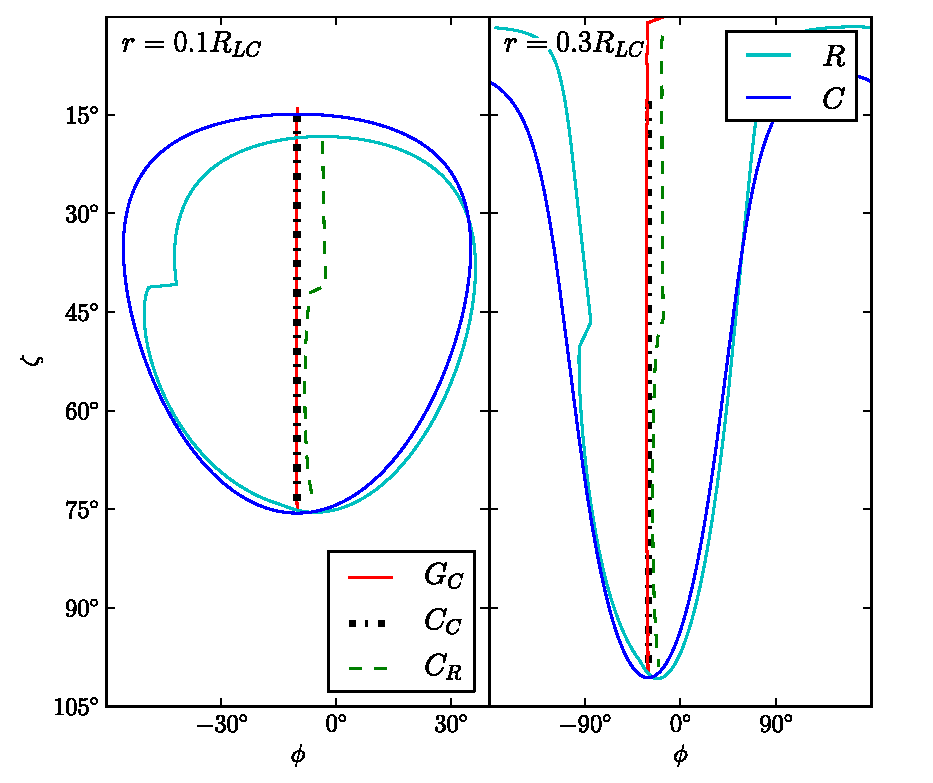
\includegraphics[width=1\textwidth]{chapters/BCWlimitations/figures/imageCaps.eps}
\caption[Pulse phase estimates for $\alpha=45^\circ$, $\phi(\zeta) = 0$
for two different altitudes, $r=0.1R_{\rm{LC}}$ and $r=0.3R_{\rm{LC}}$]{Pulse phase estimates for $\alpha=45^\circ$, $\phi(\zeta) = 0$ 
for two different altitudes, $r=0.1R_{\rm{LC}}$ and $r=0.3R_{\rm{LC}}$.
$G_{\rm{C}}$: Peak phase from maximum of simple Gaussian intensity weighting.
$C_{\rm{C}}$: Peak phase from center of cap edges (circular cap).
$C_{\rm{R}}$: Peak phase from center of cap edges (retarded dipole cap).}
\label{fig:Plotcap}
\end{center}
\end{figure}

	Not unexpectedly, Figure~\ref{fig:Plotcap} shows that the pulse phase is 
more sensitive to the details of the open zone geometry for a conal emission zone.
The offsets shown there illustrate the effect of the retarded potential field
line flaring at high altitude. To this should be added the uncertainties associated 
with identifying the magnetic axis phase in the presence of patchy conal emission and
non-dipole field structure (for millisecond pulsars). Nevertheless, as we shall show, a substantial
fraction of the phase offset is insensitive to the choice of cap center, and can
be corrected.

\subsection{`Fitting' an RVM curve}

The retarded dipole field structure increasingly departs from the point dipole
as the scaled emission height $r=r_{\rm{em}}/R_{\rm{LC}}$ approaches unity. Thus
if one fits polarization data for a low altitude emitter with the RVM model, the 
fit parameters $\alpha_{\rm{f}},\zeta_{\rm{f}}$, and $r_{\rm{f}} = \Delta \phi_{\rm{f}}/4$ at the $\chi^{2}$ minimum will be
good approximations to the real values $(\alpha_{\rm{r}}, \zeta_{\rm{r}}, r_{\rm{r}})$. For modest $r_{\rm{r}}$
the RVM fit will absorb the sweep shape departures, (correctably) biasing the
parameter estimates, while retaining reasonable $\chi^{2}$. At large altitude, the
$\chi^{2}$ will be poor, the parameters will be uncorrectably far from the true
values and a fit to a detailed numerical model will be required. The key question
is how, with realistic errors $\sigma_{\rm{PA}}$, the unabsorbed distortion grows.

	We use our estimated $\sigma_{\rm{PA}}$ to construct a `$\chi^2$' weighted 
departure of the RVM model from the detailed retarded field simulation. This is the
weighted systematic error caused by the inability of the RVM model to absorb
the detailed shape of the retarded field curve. In a real observation, additional
statistical measurement errors would increase `$\chi^2$' above our model value,
especially for small $r$. Any unmodeled physical effects should additionally increase
the value of `$\chi^2$' above $\sim 1$/(degree of freedom) at the minimum.
Observers typically adopt the increase $\Delta \chi^2=\chi^2-\chi_{\rm{min}}^2$ to
estimate the confidence intervals on the fit parameters. We are free to do the 
same here, since our prescription weights appropriately show where the model 
parameters are most sensitive to the data values.  We have confirmed this by 
fits to a series of Monte Carlo simulations of polarization angle data with added statistical errors,
showing that $\Delta \chi^2$ follows the usual distribution for the appropriate 
numbers of degrees of freedom. 

\section{Correcting for Bias in the RVM Height Estimates}
\label{sec:correctionRVM}





\begin{figure}[t!!]
\begin{center}
%\includegraphics[width=.7\textwidth]{BCWlimitationsFigures/totDirFitPhi.eps}
\includegraphics[width=\textwidth]{chapters/BCWlimitations/figures/totDirFitPhi.eps}
\caption[Altitude limits for effective RVM fits]{
Altitude limits for effective RVM fits.  Each panel shows the distribution
of simulated model fits (color bar) in offset from the true altitude as a function 
of fit altitude $r_{\rm{f}}/R_{\rm{LC}}$. The dark band shows the systematic bias in the 
fit offset. The four panels are for different assumptions about the cap 
illumination and method of estimating the true phase of $\phi=0$.
$E_{\rm{B}}$: Perfect knowledge of the location of magnetic axis in phase, without the use of an intensity model.
$G_{\rm{C}}$: Simple Gaussian intensity peak, $\phi=0$ inferred from the altitude dependent shift of $I_{\rm{max}}$. 
$C_{\rm{C}}$: Peak intensity assigned to the center of a double pulse from edges of an open zone circular cap footpoints.
$C_{\rm{R}}$: Peak intensity assigned to the center of a double pulse from edges of an open zone above the detailed retarded dipole cap.
The green curve shows our estimate of the bias, Equation \ref{eq:genCor}.
}
\label{fig:totDirFitPhiBCWlim}
\end{center}
\end{figure}


	Our principal goal here is to test the utility of standard RVM fits and
to provide a prescription to allow these fits wider applicability for pulsars
with high altitude emission. To do this we compare the RVM fit estimate $r_{\rm{f}}$ with
the simulated value $r_{\rm{r}}$. Since the mapping is not simple, statements about
ranges of validity are perforce statistical. This makes our answers mildly
sensitive to the distribution in the underlying pulsar population. Here
we assume that our parent 
pulsar population has isotropically distributed inclination and viewing angles,
ie. Prob$(\alpha)\propto {\rm sin}(\alpha)$, Prob$(\zeta) \propto {\rm sin}(\zeta)$
while the altitude is distributed uniformly on $0\le r_{\rm{r}}\le 0.3$. Note that we
only {\it observe} a usable polarization sweep if a pulsar produces a minimum
number of phase bins (here $\Delta \phi_{\rm{obs}}>0.1$). In turn,
this means that our observable pulsar population is biased toward modest
$|\beta| = |\alpha-\zeta|$.

	We generate a set of pulsar models and apply the RVM fits. This delivers
a set of observables ${\alpha_{\rm{f}}, \zeta_{\rm{f}}, r_{\rm{f}}; \sigma_{\alpha_{\rm{f}}}, \sigma_{\zeta_{\rm{f}}}, \sigma_{r_{\rm{f}}}}$
where the fit values are determined by $\chi^2$ minimum and the error ranges
are estimated from the curvature of the $\chi^2$ surface. An observer presented
with this set of measurements must infer the original pulsar properties.

	Focusing here on the height measurement, we test the systematic bias in
the RVM estimate. For best comparison with the BCW assumptions, we work with
the height determined from the phase lag measured from the peak of a Gaussian pulse
centered on the magnetic axis. In Figure~\ref{fig:totDirFitPhiBCWlim}, the color scale
represent the number of pulsars in the simulated population
at a given altitude derived from fitting RVM versus the difference between fitted and
real altitude. Figure~\ref{fig:totDirFitPhiBCWlim} shows that $r_{\rm{f}}$ increasingly underestimates
$r_{\rm{r}}$ at increasing altitude. A simple formula to provide improved height estimates 
$r_{\rm{f}}'$ from RVM fits is then
\begin{equation}\label{eq:genCor}
r_{\rm f}' = r_{\rm f}+ 0.2 (r_{\rm f}/0.5)^2,
\end{equation}
as plotted in Figure~\ref{fig:totDirFitPhiBCWlim}.  The line fits best to the darkest 
ridge (the ridge that contains a majority of simulated pulsars) 
for the models using the maximum of a simple Gaussian intensity peak ($G_{\rm{C}}$)
and the center of the cap edges for a circular cap ($C_{\rm{C}}$).  For the case using
the center of the cap edge for a retarded dipole cap ($C_{\rm{R}}$), the line
slightly under-predicts the 
darkest ridge and does not capture the behavior of the 
second ridge which is caused by the shift of the central line from the cap notch
(see Figure~\ref{fig:Plotcap}).  We can (unrealistically) assume that 
we know where in phase the magnetic axis 
is located and calculate the altitude from the shift in polarization directly.  Inaccuracies 
in altitude are then from Equation~\ref{eq:BCWPhi} alone.  
With the assumption of perfect knowledge of 
the magnetic axis ($E_{\rm{B}}$), we see the departure from the BCW formulation occurs 
at lower altitudes.  Apparently, the estimate $\Delta \phi=-2r_{\rm{f}}$ 
for the peak intensity shift preserves good accuracy to higher altitude 
than the $\Delta \phi=+2r_{\rm{f}}$ shift of the polarization
sweep, especially when the intensity arises from a circular cap.

\begin{figure}[htbp]
\begin{center}
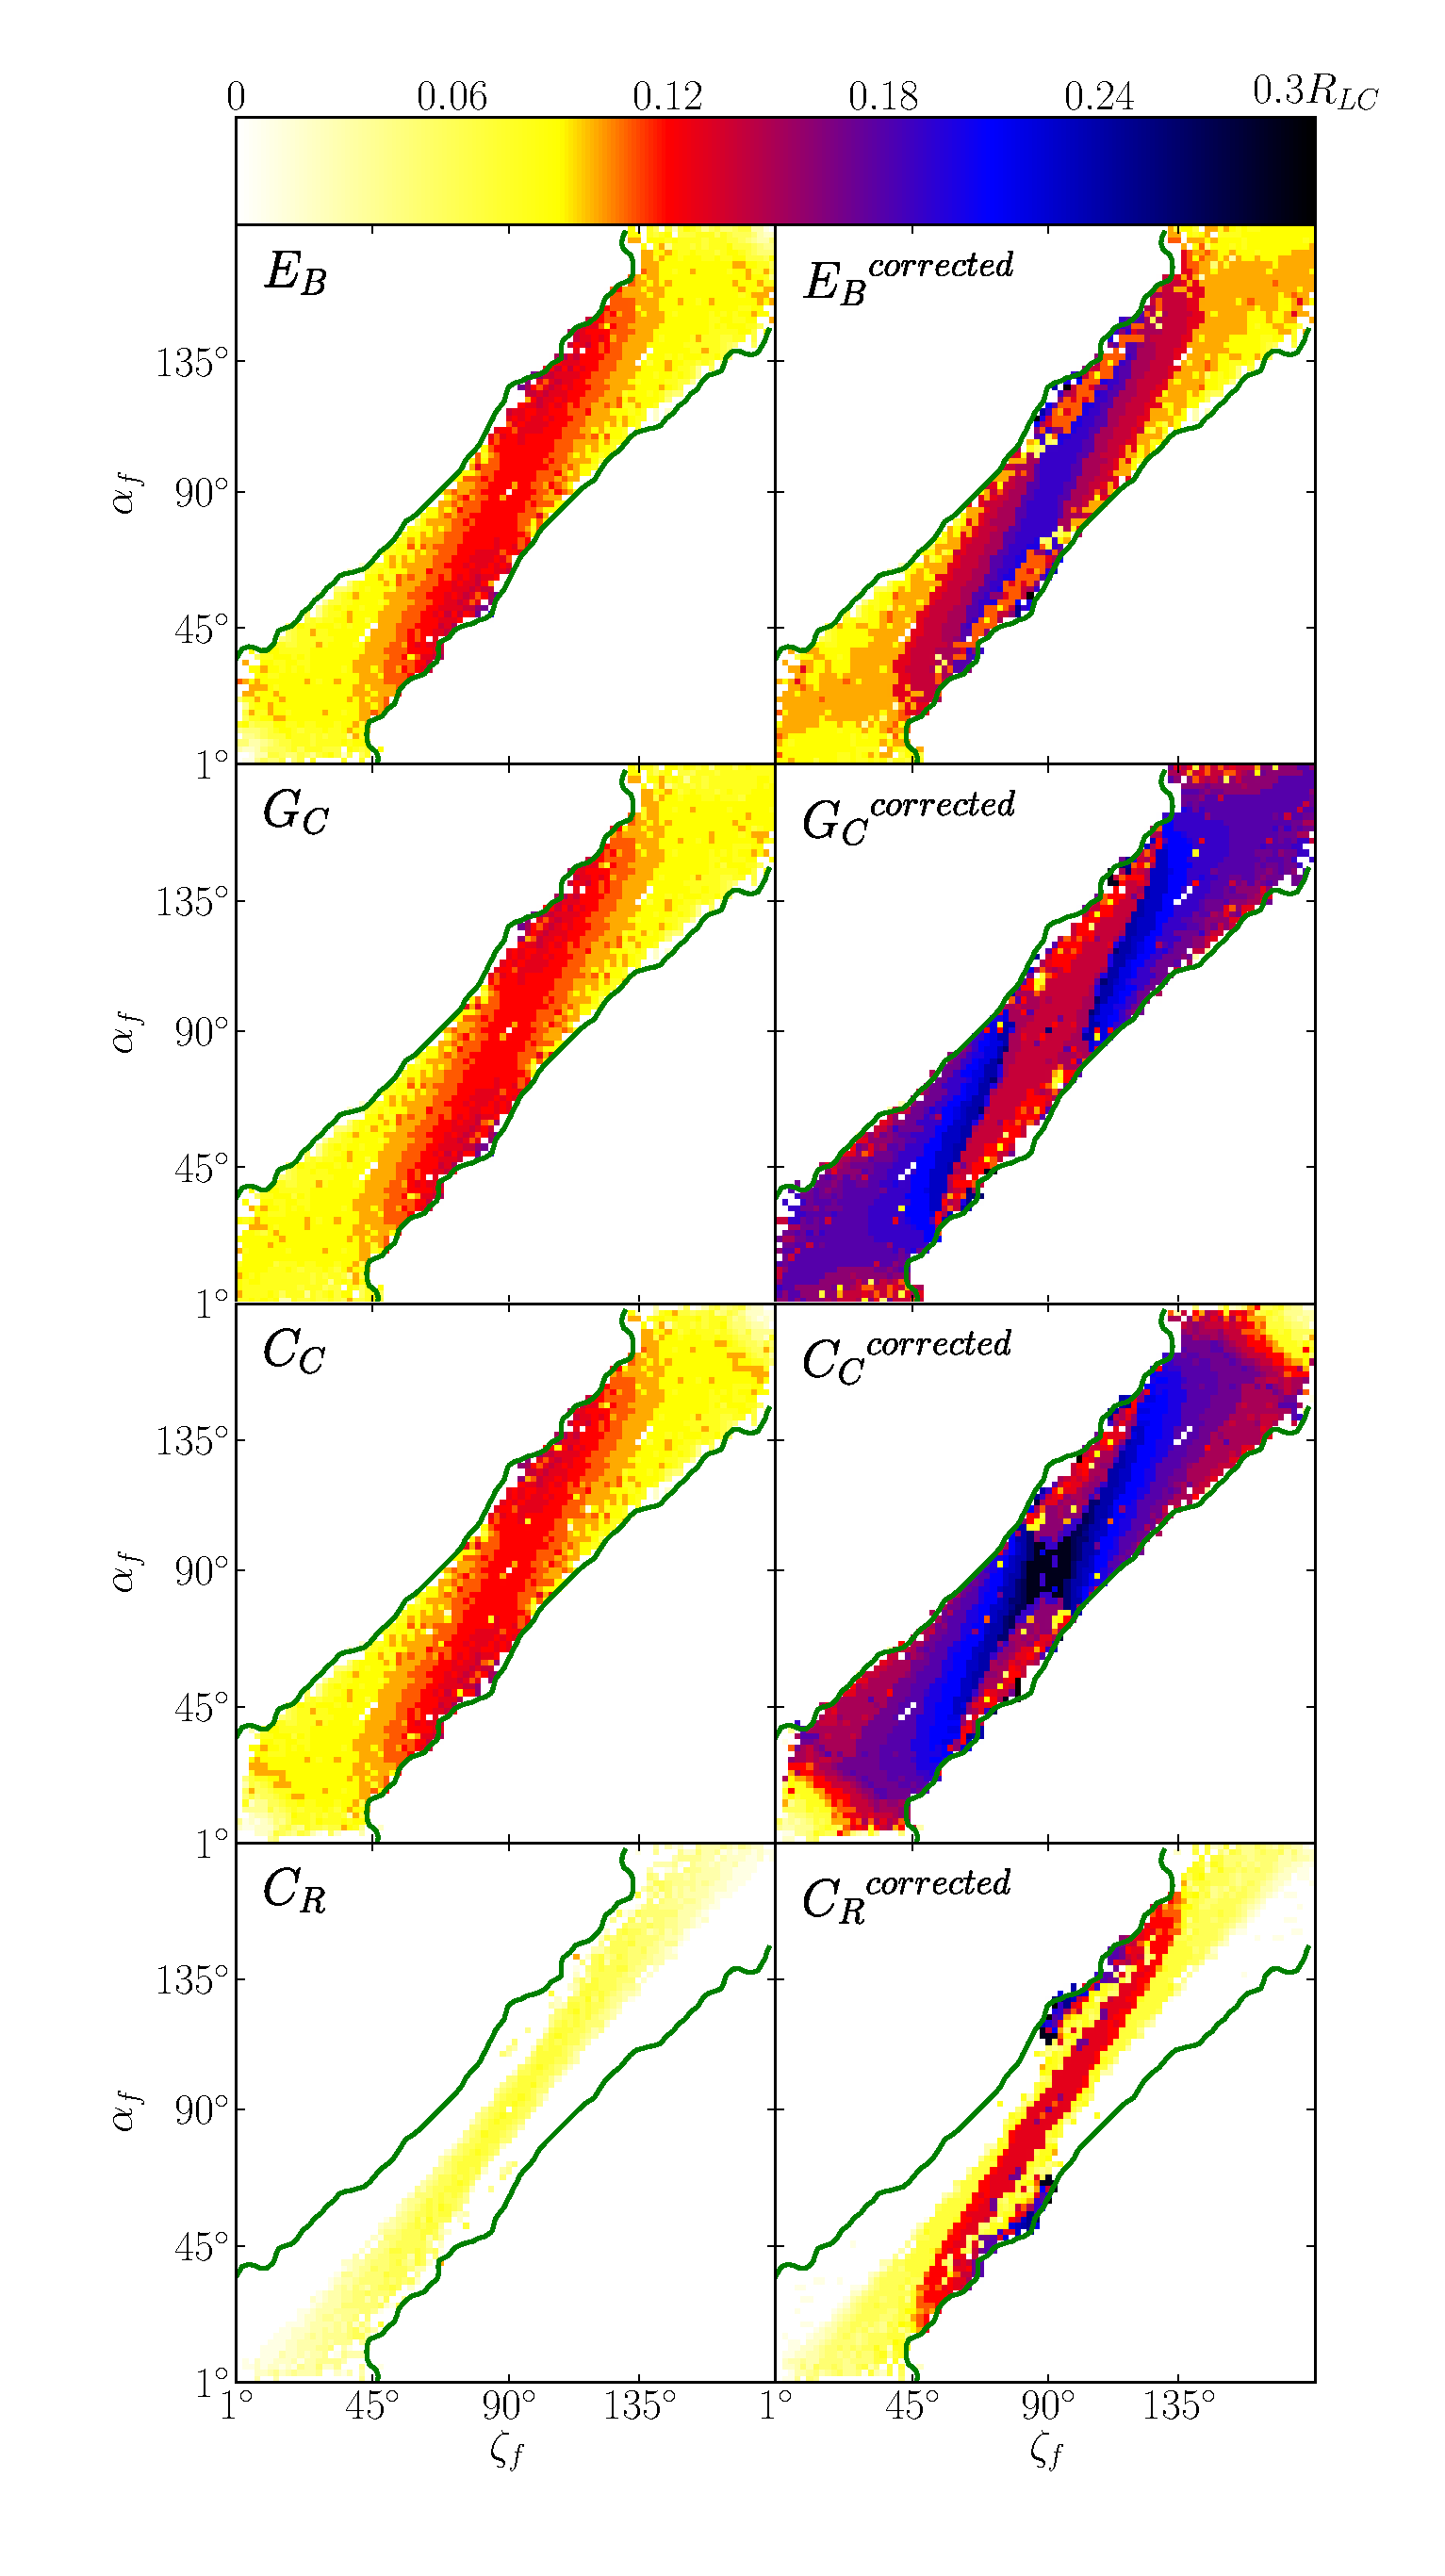
\includegraphics[width=.65\textwidth]{chapters/BCWlimitations/figures/SmapGenCorrected8V2.eps}
\caption[Maximum useful $r_{\rm{f}}$ altitude (color bar) in the ($\alpha_{\rm{f}}$, $\zeta_{\rm{f}}$) plane for four
assumptions about the pulse intensity beam shape.]{
Maximum useful $r_{\rm{f}}$ altitude (color bar) in the ($\alpha_{\rm{f}}$, $\zeta_{\rm{f}}$) plane for four
assumptions about the pulse intensity beam shape (see text for our criterion
for good fit accuracy).  Left: BCW estimates before
correction. Right: corrected heights using Equation~\ref{eq:genCor}.
Green contours indicate the area where at least fifty simulated pulsars
were fit to an ($\alpha_{\rm{f}}$,$\zeta_{\rm{f}}$) pair.
}
\label{fig:SmapCorrected8}
\end{center}
\end{figure}

	In practice, the height offset depends on the geometrical angles 
$(\alpha, \zeta)$. In addition, the height estimate is affected by uncertainty
in estimating the polarization sweep lag, i.e. in determining the phase of the pulse 
(or equivalently the phase of the magnetic axis). These effects are shown in 
Figure~\ref{fig:SmapCorrected8}. For each panel we show, as a function of the estimated angles
$(\alpha_{\rm{f}}, \zeta_{\rm{f}})$, the maximum height (color bar) at which the estimated altitude is
accurate. For the estimate to be useful, we require that $r_{\rm{r}}$ lies in
the range $r_{\rm{f}}\pm\sigma_{r_{\rm{f}}}$ for a large fraction (99\%) of the observable
model pulsars. At small altitude this is always true. At large altitude
the distortion due to the retarded field structure causes increasing
departure from the BCW estimate. Once too small a fraction of models produce
useful fits, the BCW approximation `breaks down'.  Lowering the required fraction
does not drastically change the results seen in Figure~\ref{fig:SmapCorrected8}, since
the fraction of failing models increases very rapidly with fit altitude. Also shown
is a green contour that marks the area where the bins contain at least
fifty simulated pulsars.  Uncolored bins are where the BCW approximation is
inaccurate at the lowest altitude.  The contours are independent 
of the intensity model (the contours are the same for each model) because
the $\alpha_{\rm{f}}$, $\zeta_{\rm{f}}$ bin
depends only on the polarization sweep which is calculated independently
of the intensity model.

A strong dependence between the break-down altitude and $\alpha_{\rm{f}}$ and $\zeta_{\rm{f}}$ exists as can 
be seen in Figure~\ref{fig:SmapCorrected8}.  This is not due to any
difficulty in finding the phase center but arises from the nontrivial relation between
the shift in the maximum sweep of the polarization and the geometry angles.
In Figure~\ref{fig:SmapCorrected8}, we can see that for $\alpha_{\rm{f}}$ and $\zeta_{\rm{f}}$
further from $90^\circ$, BCW tends to break down at a lower altitude.  
The shift in the maximum sweep of the polarization angles for these values is smaller
than predicted by the BCW model. Since the BCW model has no dependence on
$\alpha$ and $\zeta$, it is not surprising that the break-down altitude has 
a dependence on these angles.

The panels show the maximum useful height for
four different estimates of the phase lag: (top-to-bottom) perfect knowledge of
the magnetic axis, a Gaussian pulse peaked on the magnetic axis field line, a 
`conal' pulse from a field lines with a circular cap on the star and a `conal' pulse with
a cap determined by the detailed open zone of the retarded vacuum solution. 
Notice that most observed pulsars have modest $|\beta|=|\zeta-\alpha|$, and 
are close to the diagonal.
The right panels show the equivalent maximum useful height when the
estimate has been corrected according to Equation \ref{eq:genCor}. While the uncorrected
estimates for the Gaussian pulse peak model are useful 
only to an average (over $\alpha_{\rm{f}}$ and $\zeta_{\rm{f}}$) height of $\overline{r_{\rm{f}}}=0.11R_{\rm{LC}}$, the corrected
estimates are usable to higher altitudes (reaching $r_{\rm{f}}'\sim 0.3$ for the commonly
observed case of near-orthogonal rotators) with an average of $\overline{r_{\rm{f}}}=0.22R_{\rm{LC}}$.
Again, corrected
RVM estimates from a model radio pulse do better than estimates
assuming perfect knowledge of the magnetic axis, since the retarded potential
phase shifts are a fractionally larger contribution to the phase offset in this
case. 
\begin{figure}[htbp]
\begin{center}
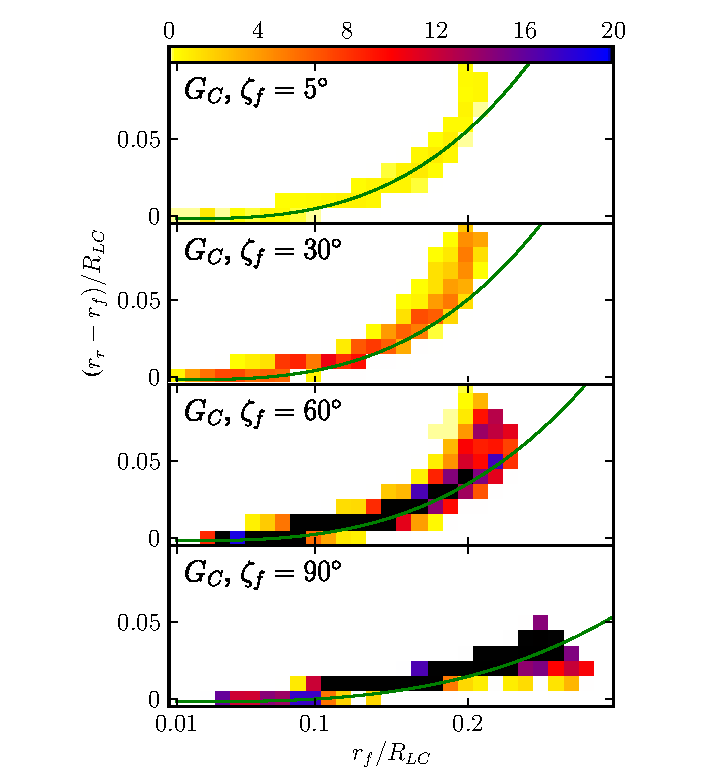
\includegraphics[width=.9\textwidth]{chapters/BCWlimitations/figures/zetaResmagMin.eps}
\caption[Altitude limits for effective RVM fits]{
Altitude limits for effective RVM fits.  Each panel shows the distribution
of simulated model fits (color bar) in offset from the true altitude as a function
of fit altitude $r_f/R_{\rm{LC}}$ for different $\zeta_{\rm{f}}$, assuming a simple Gaussian intensity peak, 
$\phi=0$ inferred from the altitude dependent shift of $I_{\rm{max}}$.
For these plots, the simulated pulsar population has been 
summed over $\alpha_{\rm{f}}$ to emphasize the dominance of $\zeta_{\rm{f}}$ in the correlation.
The green curve shows our estimate of the bias with dependence on 
$\zeta_{\rm{f}}$, Equation \ref{eq:zetaCor}.
}
\label{fig:zetaResmagMin}
\end{center}
\end{figure}

	We can improve the heuristic correction function by including the
viewing geometry. The bulk of the sensitivity is evidently due to $\zeta_{\rm{f}}$,
as illustrated by the relatively small dispersion of the $r_{\rm{f}}$ error for
individual $\zeta_{\rm{f}}$ slices (see Figure~\ref{fig:zetaResmagMin} for
a Gaussian central pulse).
Accordingly, we have made an alternate corrected height estimate
\begin{equation}\label{eq:zetaCor}
r_{\rm{f}}' = r_{\rm{f}}+ [0.3 + 0.7 |\cos(\zeta)| ] (r_{\rm{f}}/0.5)^{3} 
\end{equation}
where $r_{\rm{f}}=\Delta \phi/4$, as usual. This greatly extends the range for which
a simple RVM height estimate can be used (Figure~\ref{fig:SmapCorrected4}). This estimate, based
on a Gaussian radio pulse emitted along the swept back magnetic axis, is
in general the best function for an observer to use with no other information. It provides significant
improvement in the emission height accuracy for the circular cone pulse profiles.

\begin{figure}[t!!]
\begin{center}
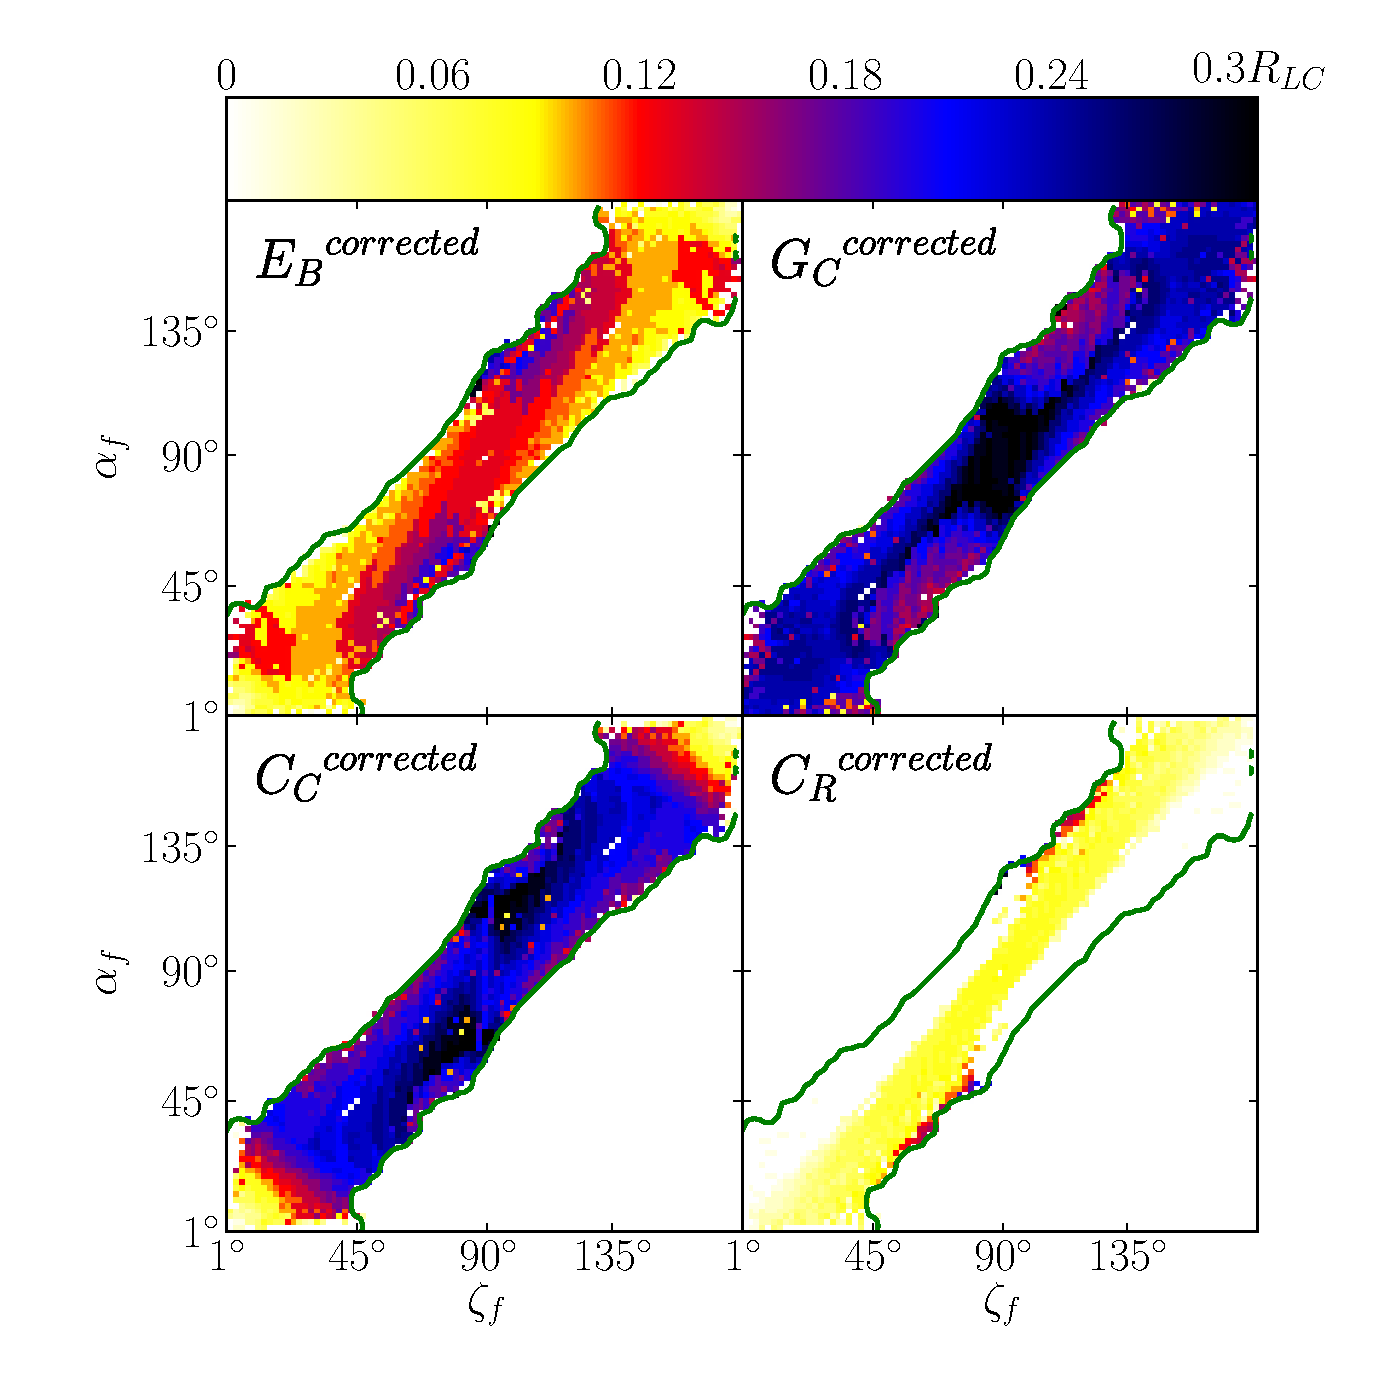
\includegraphics[width=.9\textwidth]{chapters/BCWlimitations/figures/SmapCorrected4V2.eps}
\caption[Maximum altitude for accurate height estimates (color bar) in the
($\alpha_{\rm{f}}$, $\zeta_{\rm{f}}$) plane, after applying Equation \ref{eq:zetaCor}]{Maximum altitude for accurate height estimates (color bar) in the 
($\alpha_{\rm{f}}$, $\zeta_{\rm{f}}$) plane, after applying Equation \ref{eq:zetaCor}
(see text for our criterion for good fit accuracy).
Note that the improvement is best for a circular (Gaussian or conal) cap.
Green contours indicate the area where at least fifty simulated pulsars
were fit to an ($\alpha_{\rm{f}}$,$\zeta_{\rm{f}}$) pair.
}
\label{fig:SmapCorrected4}
\end{center}
\end{figure}

	Of course if one has reason to believe that a particular pulse 
profile shape is more accurate, a different correction function may be
preferred. For example if one had a double pulse arising from the open zone edges ($C_R$) and
had high confidence that this pulse filled the retarded vacuum dipole open
zone, one would correct by
\begin{equation}\label{eq:zetaCor2}
r_{\rm{f}}' = r_{\rm{f}}+ [0.3 +2 |\cos(\zeta)|^{2} ] (r_{\rm{f}}/0.5)^{3}.
% a bit cleaner, but check that this is indeed the correct form  -- RWR
\end{equation}
This formulation raises the average over $\alpha_{\rm{f}}$ and $\zeta_{\rm{f}}$ of
the maximum useful height from $\overline{r_{\rm f}}=0.05R_{\rm{LC}}$ with no correction to 
$\overline{r_{\rm{f}}}=0.15R_{\rm{LC}}$.

	In general, we recommend that when an observer fits an RVM model to pulsar
data, obtaining viewing angle and polarization sweep lag measurements,
they correct their height estimate using Equation \ref{eq:zetaCor}.  This is 
particularly useful whenever the RVM fit appears statistically adequate,
but the resulting phase lag suggests a significant emission height.
The change to the estimated height will be small for $r_{\rm{f}} < 0.2$,
but the accuracy of the resulting estimate will be greatly increased.

	Of course, whenever $\chi^2$/DOF $\gg1$ at the fit minimum, it is a sign
that the model is inadequate. In many cases, this will be due to 
unmodeled orthogonal mode jumps and intervening scattering \citep{karastergiou2009complex},
higher order multipoles, etc. However, for large altitudes and
multi-altitude emission the effects of sweep back and the formation
of caustics (which dominate $\gamma$-ray light curves) become dominant.
The observer should be aware that large $\chi^2$ at the fit minimum
can signal such effects and, when the inferred altitude is large, consider 
fitting the data to numerical models of 3-D pulsar magnetospheres.

\section{Height Calculation from Shift in $\psi$}
\label{sec:heightFromPsi}

We can alternatively estimate $r_{\rm{f}}$ and errors using the shift in $\psi$ \citep{hibschman2001polarization},
\begin{equation}\label{eq:HA}
\Delta\psi \approx \frac{10}{3} r \cos(\alpha) \left[\frac{3}{8}+\frac{5}{8} \cos(\zeta-\alpha)\right]\\
- \frac{47}{18} r \sin(\alpha) \sin(\zeta-\alpha)
\end{equation}
or, in the small $|\beta|=|\zeta-\alpha|$ limit, $\Delta\psi\approx \frac{10}{3} r \cos(\alpha)$.
As before, we compute the residual, $r_{\rm{r}}-r_{\rm{f}}$, as a function of $\alpha_{\rm{f}}$, $\zeta_{\rm{f}}$, 
and $r_{\rm{f}}$. To estimate an emission height from the polarization shift in $\phi$,
one needs an estimate for $\phi=0$, e.g. from a pulse peak intensity model; no such intensity
model is needed if we have a measurable shift in $\psi$.
The increase with $r_{\rm{f}}$ are shown in Figure~\ref{fig:totDirFitPsy},
where the left panel uses the small $\beta$ limit while the right uses the full formula.
As for the $\Delta\phi$ estimate, the errors increase with $r_{\rm{f}}$. However here, even
when the full Equation \ref{eq:HA} is used, the corrections show a substantial spread.
In fact the uncorrected formula proves accurate ($|r_{\rm{f}}-r_{\rm{r}}|$ within $\sigma_{r_{\rm{f}}}$ 99\% of the
time) only for $\overline{r_{\rm{f}}} < 0.08$ (where $\overline{r_{\rm{f}}}$ is again 
the average over $\alpha_{\rm{f}}$ and $\zeta_{\rm{f}}$)
and for $\zeta_{\rm{f}} <60^\circ$ or $\zeta_{\rm{f}} >120^\circ$. 
For near-orthogonal rotators the estimate is unreliable at the lowest altitudes.

\begin{figure}[t!!]
\begin{center}
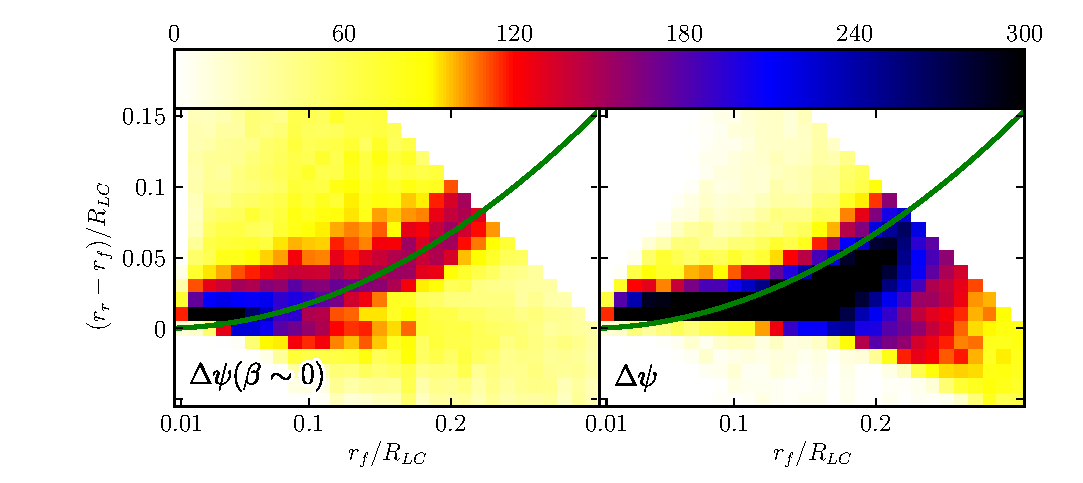
\includegraphics[width=.9\textwidth]{chapters/BCWlimitations/figures/totDirFitPsy.eps}
\caption[Altitude limits for effective RVM fits using the shift in $\psi$]{
Altitude limits for effective RVM fits using the shift in $\psi$.  Each panel shows the distribution
of simulated model fits (color bar) in offset from the true altitude as a function
of fit altitude $r_{\rm{f}}/R_{\rm{LC}}$. The dark band shows the systematic bias in the
fit offset. 
The residual is more scattered when the altitude is measured from 
the shift in $\psi$ instead of the shift in $\phi$ of the polarization
sweep. 
On the left is the residual using the small $|\beta|$ limit.
The green curve shows our estimate of the bias from the 
shift in $\psi$, Equation \ref{eq:DPsi1}.
}
\label{fig:totDirFitPsy}
\end{center}
\end{figure}

	A heuristic correction to the $\Delta \psi$ estimate for Equation \ref{eq:HA} can be made
for $\zeta_{\rm{f}} <60^\circ$ or $\zeta_{\rm{f}} >120^\circ$
\begin{equation}\label{eq:DPsi1}
r_{\rm{f}}' = r_{\rm{f}}+ 0.4 (r_{\rm{f}}/0.5)^{2}
\end{equation}
which allows accurate estimates to $\overline{r_{\rm{f}}}=0.12R_{\rm{LC}}$. Including the $\zeta$ dependence,
\begin{equation}\label{eq:DPsi2}
r_{\rm{f}}' = r_{\rm{f}}+ [0.2 +0.1 |\cos(\zeta)|^{2}] (r_{\rm{f}}/0.5)^{2}
\end{equation}
raises the useful range to $\overline{r_{\rm{f}}}=0.18R_{\rm{LC}}$. Considering that the correction 
for the common orthogonal rotator case is especially poor, and that it is often 
difficult to infer the intrinsic $\psi_0$,
height estimates from the phase shift remain much more useful.

\section{Pulse Width Dependence on Emission Height}\label{sec:rW}
\label{sec:heightFromWidth}

	Since the field lines flare in the open zone, the full phase width $W$ of the
observed radio pulse can also be checked against the expected radio emission
altitude. The standard prescription assumes a circular cap and static dipole field
lines to infer a minimum height
\begin{equation}\label{eq:rW}
r_{\rm{W}}=\frac{4}{9}\arccos^{2}\left[\cos(\alpha)\cos(\zeta)+\sin(\alpha)\sin(\zeta)\cos\left(\frac{W}{2}\right)\right].
\end{equation}
In Figure~\ref{fig:totDirFitW} we show that the retarded dipole field flares
{\it more} than predicted by this simple formula and hence the minimum height
in Equation \ref{eq:rW} is an {\it over}-estimate. Thus, in general, lower
altitudes are consistent with a given observed pulse width than suggested by this
formula. Moreover, we expect that the general effect of currents in the magnetosphere
will be to increase the foot-point angles of the open zone.
This further increases the allowed
$W$ at a given height.

\begin{figure}[t!!]
\begin{center}
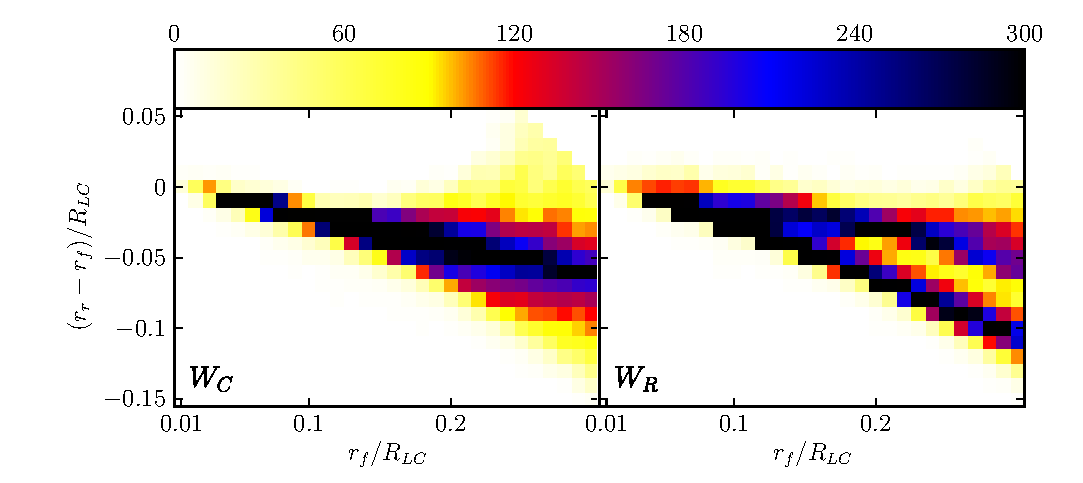
\includegraphics[width=.9\textwidth]{chapters/BCWlimitations/figures/totDirFitW.eps}
\caption[Altitude limits for effective pulse width]{
Altitude limits for effective pulse width.  Each panel shows the distribution
of simulated model fits (color bar) in offset from the true altitude as a function
of fit altitude $r_{\rm{f}}/R_{\rm{LC}}$. 
$W_{\rm{C}}$: Circular cap. $W_{\rm{R}}$: Retarded dipole cap.
The simple static dipole formula overestimates the altitude needed 
to accommodate a given pulse with $W$ in the open zone. The error depends
on the viewing geometry $\alpha$ and $\zeta$, and bifurcates for the `notched'
cap of the formal retarded potential open zone.
}
\label{fig:totDirFitW}
\end{center}
\end{figure}

In general, larger widths are still most easily accommodated at large $r$ or 
small $\alpha$, but sweep-back and magnetospheric currents substantially weaken 
the minimum altitude constraints from the commonly used Equation \ref{eq:rW}. 
Given the large sensitivity to the details of the open zone volume and the presently
unknown effect of magnetospheric currents, it is not worth developing corrections to
this formula.



\section{Conclusions; Examples from Literature}

	We conclude by examining a few RVM/BCW estimates of
emission height present in the literature.

In \cite{romani2011sub}, $\Delta \phi$ estimates were used to suggest
large emission heights for two young energetic pulsars. For PSR J0538+2817 the
shift gives $r_{\rm{f}}=0.15R_{\rm{LC}}$, but RVM fitting only weakly constraints $\zeta$.
Applying Equation \ref{eq:genCor}, we would infer $r^\prime_{\rm{f}} = 0.17 R_{\rm{LC}}$,
a small, but significant increase which makes it easier to accommodate the
large observed pulse width. Similarly PSR J1740+1000 gives $r_{\rm f}=0.12R_{\rm{LC}}$.
Here we constrain $\zeta=80^{\circ}$ to $130^{\circ}$,
so that the corrected fit altitude (Equation \ref{eq:genCor} or Equation \ref{eq:zetaCor}) is 
$r^\prime_{\rm{f}}=0.13R_{\rm{LC}}$, again a small but statistically significant increase.


	For millisecond pulsars the effects can be larger. For example, \cite{keith2012high} 
find that RVM fitting can be usefully applied to several 
recycled pulsars. PSR J1502-6752 (P=26.7\,ms) is a mildly recycled
pulsar for which the phase lag implies $r_{\rm{f}}=0.2R_{\rm{LC}}$. With no significant $\zeta$
constraints, we apply Equation \ref{eq:genCor} to infer a 16\% altitude increase
to $r^\prime_{\rm{f}}=0.23R_{\rm{LC}}$. Similarly PSR J1708-3506 ($P=4.5\,$ms) has a phase shift 
implying $0.19R_{\rm{LC}}$, which we correct to $0.21-0.22 R_{\rm{LC}}$. For this pulsar,
a naive application of the pulse width formula (\ref{eq:rW}) gives altitudes of 
$r_{W_{10}}\simeq0.65R_{\rm{LC}}$ (10\% peak width). 
However, the increased $r^\prime_{\rm{f}}$ and decreased pulse width height
from sweep-back effects (Figure~\ref{fig:totDirFitW}), along with additional current-induced
open zone growth, make it likely that the pulse width can be accommodated at the corrected height.


 \cite{keith2012high} also report a RVM/BCW height $r_{\rm{f}}= 0.44R_{\rm{LC}}$ for
the P=2.7\,ms pulsar PSR J1811-2404, along with well constrained viewing angles of
$\alpha=89.7^{\circ}$ and $\beta=21^{\circ}$. While our full analysis does
not cover this altitude, as Figure~\ref{fig:SmapCorrected4} shows the corrections
of Equation \ref{eq:zetaCor} give a very high accuracy for orthogonal
rotators viewed near $90^\circ$.  Note in Figure~\ref{fig:zetaResmagMin}, bottom
panel, that the correction function is nearly linear thus extrapolation to 
somewhat higher values may be justified.  Naively applying this correction we get
$r_{\rm{f}}'=0.81R_{\rm{LC}}$. We certainly cannot trust this value in detail since plasma 
effects and other perturbations may be relevant at such altitudes.  However, the
correction is certainly large and it brings the expected height up to an altitude 
where the very wide observed radio pulse, and the likely detection of emission 
from both open zones, can be easily accommodated.
Certainly simple RVM/BCW fitting is inadequate for this pulsar and one
should use a detailed model for the high altitude field geometry.



\bigskip
\bigskip

	Our exercise extends the range of utility of RVM-fit polarization
sweeps for inferring the altitudes of radio pulsar emission. For fit altitudes
less than $r_{\rm{f}} = 0.25 R_{\rm{LC}}$ the corrections are not large, but they are
systematic and, for high S/N data localizing the phase of maximum polarization
sweep, they can be highly significant. We thus believe it is worth applying our recommended
correction. For larger altitudes the corrections grow rapidly, but we caution
that as one approaches the light cylinder, current-induced distortions
should increase and, except for near-orthogonal rotators, one would expect the RVM
formulae to provide a poor fit in any case. Fitting to detailed numerical models
is then preferred. In all cases the dominant residual uncertainty is likely in
locating the phase of the radio pulse.
We also checked the use of absolute polarization axis position angles
and pulse width to constrain the emission height. Here the difficulties in
establishing the unperturbed $\psi_0$ and the expected distortions of the open zone
boundaries by currents, etc. make the estimates much less useful. Nevertheless,
we have shown that the effects of sweep-back do go in the direction of reconciling
observed pulsar properties to a consistent emission height: larger heights are
inferred by a given $\Delta \psi$ shift and larger pulse widths can be accommodated
at a given height. We feel, however, that the corrections are less quantitative
than for $\Delta \phi$.

	In sum, since observers will continue to apply analytic RVM fits
to pulsar polarization data, by applying our recommended 
correction (Equation~\ref{eq:zetaCor}), these results
can continue to give accurate height estimates to $\le 0.3 R_{\rm{LC}}$. At higher heights
which will be common for millisecond pulsars, a fit to more detailed numerical
models is likely warranted.

\acknowledgements

This work was supported in part by NASA grants NNX10AP65G and NAS5-00147.




\chapter[Energetic Pulsars]{Tackling Radio Polarization of Energetic Pulsars}
\label{chapter:tacklingPolarization}

\paperref{This section is based on work done for
``Tackling Radio Polarization of Energetic Pulsars''
\citep{craig2014tackling}}


The traditional, geometrical rotating vector model (RVM) has proved
particularly poor at capturing the polarization sweeps of the young energetic
and millisecond pulsars detected by \textit{Fermi}. We augment this model by including
finite altitude effects using a swept-back vacuum dipole geometry. By further
including the effects of orthogonal mode jumps, multiple emission altitudes, open
zone growth via y-point lowering, and interstellar scattering, we show that a wide
range of departures from RVM can be modeled well while retaining a geometrical
picture. We illustrate these effects by fitting six \textit{Fermi}-detected pulsars 
(PSR J0023$+$0923, PSR J1024$-$0719, PSR J1744$-$1134, PSR J1057$-$5226, PSR J1420$-$6048, and PSR J2124$-$3358) and 
we describe how such modeling can improve our understanding of their emission geometry.
\section{Introduction}
\label{sec:introTackling}


For pulsars emitting in the radio, the conventional assumption 
is that the electric vector position angle 
follows the projection onto the plane of the sky from 
the magnetic field line at the emission point.  
Polarization position angle curves (position angle versus pulsar phase), which we see
as the pulsar sweeps past our field of view,
are very closely related to the orientation of the magnetic field lines.
Analysis of radio polarization is a powerful tool for understanding the geometry of pulsars.
For example, polarization contains information about 
the phase of closest approach of the surface dipole axis.  
Additionally, polarization has traditionally been used to 
place strong constraints on the impact angle, the angle 
between the magnetic pole of the pulsar, and the viewing direction.
Modeling polarization should also give estimates for the geometric 
parameters $\alpha$, the angle of magnetic axes, and $\zeta$, the viewing angle.

Naively, such projections should result in smooth polarization curves 
versus the pulsar period phase, particularly when adopting a point dipole model.
We argue that zero altitude models are not appropriate for certain pulsars. 
In stark contrast, a relatively recent paper, \cite{yan2011polarization} exhibits 
the multitude of shapes that occur in millisecond pulsar polarization. 
More subtly, both polarization angle sweeps originating from zero altitude and 
polarization angle sweeps originating from a single, finite altitude can 
differ significantly in shape, although both appear smooth.  
Emission from finite altitude is a consideration for both millisecond pulsars and young pulsars.
\cite{karastergiou2007empirical} give the emission altitude of young pulsars
as $950$--$1000$ km. This emission altitude is then 
$0.02 \times 1000 / P_{\rm{ms}}$ $R_{\rm{LC}}$ in terms of the light cylinder radius.
The light cylinder radius, $R_{\rm{LC}}$, is the distance from the center of 
the neutron star at which co-rotating particles would be traveling
at the speed of light.
Since  $P_{\rm{ms}} < 100$ ms for young pulsars, their emission altitude would
be $> 0.2 R_{\rm{LC}}$, a significant fraction of the light cylinder. 
The neutron star radius in terms of light cylinder is $0.02 \times 10 / P_{\rm{ms}}$ $R_{\rm{LC}}$ 
for a neutron star radius of $10$ km.  For millisecond pulsars
with $P_{\rm{ms}} < 5$ ms, emission must come from $>0.04 R_{\rm{LC}}$, 
which is also a significant fraction of the light cylinder.

Precise modeling of millisecond pulsar and young pulsar radio 
polarization is of particular interest now because of the 
growth of $\gamma$-ray data from the \textit{Fermi Gamma-Ray Space Telescope}. 
These energetic pulsars make up the $\gamma$-ray pulsar population.
Thus, the understanding of $\gamma$-ray models can potentially 
benefit from radio polarization modeling because 
of the constraints on geometry that polarization often provides.
All pulsars considered in this paper are \textit{Fermi}-detected pulsars.

In essence, the present paper is an extension of the \cite{karastergiou2009complex}
paper in which the author shows one can produce theoretical 
polarization curves similar to those observed using 
orthogonal mode jumps and interstellar scattering. 
Here, we also allow for emission from finite altitude (numerically calculated).  
Although analytically calculated modifications exist for small altitude emission, 
such calculations contain estimates that break down at altitudes $\sim 0.1R_{\rm{LC}}$.
Our model also allows for multiple altitudes of emission.  Differences in 
altitude can explain non-$90^\circ$ position angle jumps seen 
particularly in millisecond pulsar polarization data.
Another major difference between \cite{karastergiou2009complex} and the present paper is that we 
seek to quantitatively fit the model to the data 
resulting in parameters with error bars and $\chi^2$ estimates. 
In contrast, \cite{karastergiou2009complex} was satisfied with producing polarization 
sweeps that appeared qualitatively similar to the data.
Further, using the \textit{F}-test, we compare the $\chi^2$ of the simplistic point dipole model 
and our more complex model to statistically quantify
whether the modifications are significant.
This paper is a methods paper that chooses pulsars that can 
clearly illustrate the strengths of this model; we do not tackle a large sample.

In Section~\ref{sec:RVM} of this paper, we discuss the rotating
vector model (RVM) and how the discrepancies between
data and the model demand a reevaluation of RVM.
In Section~\ref{sec:adding}, we describe the constituents of the
model in detail.  In Section~\ref{sec:fit}, we describe
the nuances of fitting the model.  Section~\ref{sec:ypt}
focuses on a parameter $\rho_{\rm{ypt}}$ which we define and use heavily
in this paper and which is a measure of the extent of 
the effective open zone required by phase of emission.  We apply the model
to data in Section~\ref{sec:app}. Table~\ref{tb:pulsarParam} gives
property parameters to the pulsars analysed.

\section{Rotating Vector Model and Beyond}
\label{sec:RVM}
We will start by discussing the analytic models used for 
radio position angle polarization and their shortcomings 
and then transition into the numerical model used for this paper.
The model predominately used for radio position angle polarization
is the RVM which
was formulated by \cite{radhakrishnan1969magnetic}.  The RVM is simple
and states that pulsars are point dipoles with emission
from the surface of the neutron star.  The
analytic RVM formula for polarization angles ($\psi$) is
\begin{equation}\label{eq:RVM}
\psi=\arctan\left[\frac{-\sin(\alpha)\sin(\phi+\Delta\phi)}
{\sin(\zeta) \cos(\alpha) -\cos(\zeta) \sin(\alpha) \cos(\phi+\Delta\phi)}\right]+\Delta\psi,
\end{equation}
where the inclination angle between the rotation
axis and magnetic axis is $\alpha$, the viewing angle is
$\zeta$, and the pulse phase is $\phi$. Measures of horizontal and vertical offset
are contained in $\Delta\psi$ and $\Delta\phi$.  These are the absolute phase and position angle on the 
sky of the magnetic axis.

        \begin{table}[ht]
	\small
        \caption{Property Parameters of the Pulsars}
        \begin{center}
        {
        \begin{tabular}{lcccc}
        \hline & \\[-1em]\hline

        Name            &Period     &$R_{\rm{LC}}/R_{\rm{NS}}$     &$f$       &DM           \\%&$\tau_s$(ms)\\
			&(ms)	    &			 &(GHz)	    &(cm$^{-3}$ pc) \\
        [.3em]\hline 
        J0023$+$0923      &3.05           &12.5                    &1.649          &14.326                 %&1.9e-6      
\\ \hline
        J1024$-$0719      &5.162          &20.0                    &1.369          &6.49                   %&1.9e-10      
\\ \hline
        J1057$-$5226      &197.11         &1000                   &1.5            &30.1                   %&2.3e-8      
\\ \hline
        J1744$-$1134      &4.075          &16.7                    &1.369          &3.14                   %&3.3e-8       
\\ \hline
        J1420$-$6048      &68             &250                   &1.5 and 3      &360                    %&--            
\\ \hline
        J2124$-$3358      &4.931          &20.0                    &1.369          &4.60                   %&1.9e-7       
\\ \hline


        \end{tabular}}
        \label{tb:pulsarParam}
        \end{center}
        \end{table}



Despite its simplicity, the RVM has been applied to numerous pulsars with great
success (i.e., \citealp{lyne1988shape}; \citealp{phillips1990magnetic}; \citealp{everett2001emission}).  
These pulsars are generally old, spun-down pulsars
with long periods and low altitudes of emission.
\cite{blaskiewicz1991relativistic} (the Blaskiewicz, Cordes, \& Wassermann, or BCW model) 
modified the RVM to include
finite altitude and found that the point of fastest change
in the polarization position angle sweep will shift back in phase
due to sweep-back effects on the magnetic field lines, while the intensity
profile shifts forward in phase due to co-rotation of the particles
in the pulsar magnetosphere.  Therefore, by fitting the position angle
data to the RVM and measuring this shift, one can estimate altitude.

The BCW formula with altitude ($r$) dependence measured in $R_{\rm{LC}}$ is given by

\begin{equation}\label{eq:BCWdeltaPhi}
\psi=\arctan\left[\frac{-\sin(\alpha)\sin(\phi-2r)}
{\sin(\zeta) \cos(\alpha) -\cos(\zeta) \sin(\alpha) \cos(\phi-2r)}\right]+\Delta\psi
\end{equation}
\citep{dyks2008altitude}.

\begin{figure}[htbp]
\begin{center}
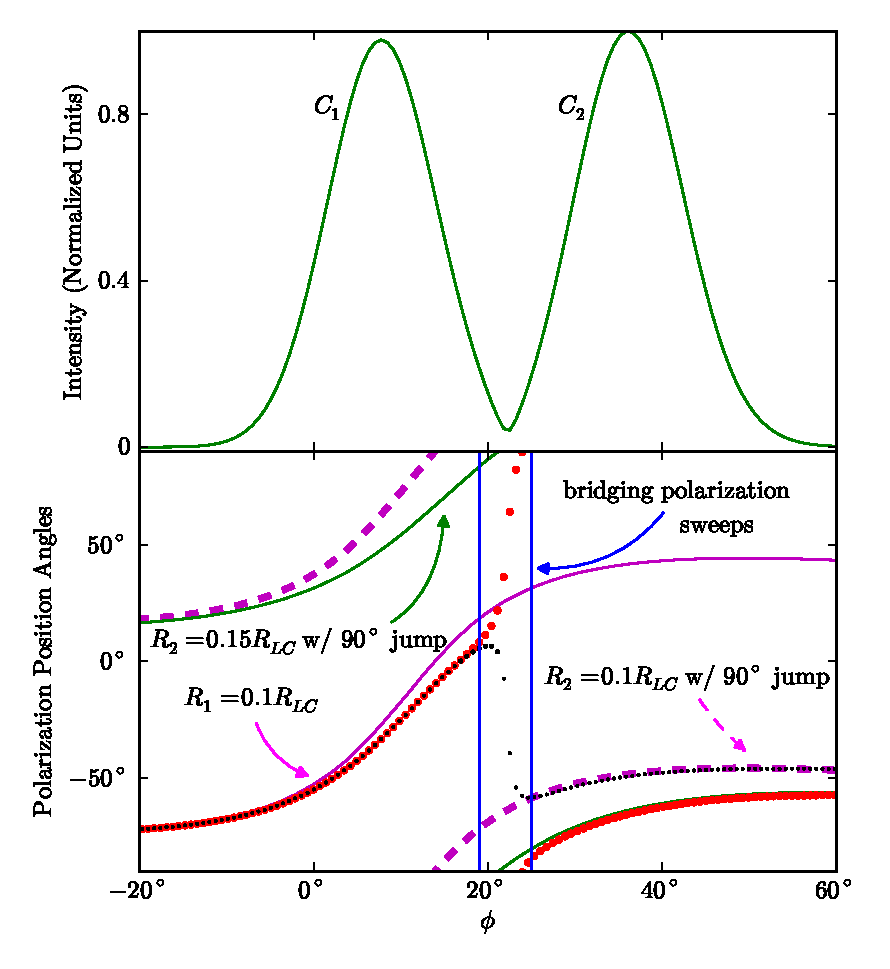
\includegraphics[scale=.7]{chapters/applicationOfNumericalModel/figures/intAndPAJexamplealpha145zeta140.eps}
\caption[Plot of model pulsar intensity and polarization sweep showing the effects of single and
multiple altitudes with a small scattering constant]{\label{fig:PlotJexampleintPA}
Plot of model pulsar intensity and polarization sweep showing the effects of single and 
multiple altitudes with a small scattering constant.
The model parameters are $\alpha=145^\circ$, $\zeta=140^\circ$, $P=5$ ms, and $\tau=0.03$ ms.
The black points are polarization position angles for a model with $R_1=0.1R_{\rm{LC}}$ for
polarization associated with intensity component $C_1$ 
and $R_2=0.1R_{\rm{LC}}$ plus an orthogonal mode jump for 
polarization associated with intensity component $C_2$.
The red points are polarization position angles for a model with $R_1=0.1R_{\rm{LC}}$ for 
polarization associated with intensity component $C_1$ 
and $R_2=0.15R_{\rm{LC}}$ plus an orthogonal mode jump for 
polarization associated with intensity component $C_2$.
Each model polarization sweep for a given component is
weighted using the Gaussian intensity profile.
Subtle changes in altitude can create drastic changes
in the direction of the bridging polarization in the phase of orthogonal mode jump.
The two Gaussian components of model intensity are equal in amplitude
but interstellar scattering effects make the first Gaussian component in 
phase ($C_1$) slightly lower in amplitude compared with the second
Gaussian component in phase ($C_2$). A phase of zero is the point
of closest encounter to the magnetic axis in the model.
}
\end{center}
\end{figure}

\begin{figure*}[t!!]
\vskip .35\textheight
\special{psfile=chapters/applicationOfNumericalModel/figures/XY.eps            hoffset=-100 voffset=-72 vscale=43 hscale=43}
\special{psfile=chapters/applicationOfNumericalModel/figures/intAndPAJexamplealpha145zeta140Wypts.eps hoffset=244 voffset=-72 vscale=43 hscale=43}
\special{psfile=chapters/applicationOfNumericalModel/figures/XZ.eps            hoffset=70 voffset=-72 vscale=43 hscale=43}
\begin{center}
\caption[Pulsar magnetic field lines at various viewing angles and a typical model polarization sweep with $\alpha=145^\circ$]{\label{fig:mfl}
Panels (A) and (B) show pulsar magnetic field lines at various viewing angles for a pulsar with $\alpha=45^\circ$.
The magenta lines are the last closed field
lines of a vacuum dipole and the solid blue lines represents the light
cylinder ($1 R_{\rm{LC}}$).  Formally, for the vacuum dipole model, the
y-point radius ($\rho_{\rm{ypt}}$), the cylindrical radius from the spin
axis at which the closed and open field lines
are adjacent, is $\rho_{\rm{ypt}}=1 R_{\rm{LC}}$.  In reality, due to finite mass and current
effects, $\rho_{\rm{ypt}}<1 R_{\rm{LC}}$.  Also plotted is the last closed field lines for
$\rho_{\rm{ypt}}=0.7 R_{\rm{LC}}$ and $\rho_{\rm{ypt}}=0.4 R_{\rm{LC}}$.  The inset plot of panel (B) shows
a close-up of the y-point area and illustrates
why this point is called the y-point.  Panel (C) shows a typical model polarization sweep with $\alpha=145^\circ$,
$\zeta=140^\circ$, and $R=0.1R_{\rm{LC}}$.  Open circles mark the expected emission phase for the model.  
Decreasing $\rho_{\rm{ypt}}$ increases the phase of emission.   A phase of zero is the point
of closest encounter to the magnetic axis in the model.
}
\end{center}
\vskip -0.2truecm
\end{figure*}



The formula is approximate and breaks down as altitude increases.  The
breakdown occurs between $\sim 0.05R_{\rm{LC}}$ and $\sim 0.12R_{\rm{LC}}$
at best, below or near altitudes expected for energetic young and
millisecond pulsars.  One can apply correction
formulae to boost the break-down altitude to $\sim 0.3R_{\rm{LC}}$,
but even these formulae are sensitive to $\alpha$ and $\zeta$
and depend on an assumed radio intensity model (\citealp{craig2012altitude}).
In essence, neither the RVM nor the BCW captures the morphological changes
in the radio polarization position angle sweep at
high altitudes which are needed to model high-energy, $\gamma$-ray emitting pulsars.

Further, the RVM produces smooth S-shaped position angle sweeps
versus phase that resemble data from older, low-energy
pulsars.  Polarization position angle data from millisecond pulsars,
on the other hand, are riddled with jumps, cusps, and sharp turns
(i.e., \citealp{yan2011polarization}; \citealp{everett2001emission})
which are absent in the RVM (the strongest
evidence that the RVM lacks essential physical features
needed to understand emission from these pulsars).  By combining
four physically motivated, data-driven ingredients (numerically calculated
finite altitude, multiple altitudes, orthogonal mode jumps, and interstellar
scattering), we hope to explain some of the features seen in the radio data
of \textit{Fermi} pulsars for which the RVM alone fails.

In the model presented in this paper, and in contrast to the RVM and the BCW, 
finite altitude polarization is calculated using
numerical computation, which avoids the approximations needed in the BCW. 
The retarded dipole presented in \cite{kaburaki1980determination} and used in \cite{Watters:2010jb}
is used in this modeling.  Particles follow magnetic field lines
to a given altitude of emission (as measured radially from the center of the 
neutron star) and, similar to the RVM, radiate tangent to the
field line.  Co-rotation and time-of-flight effects are then applied when emission from the lab
frame is projected onto the plane of the sky 
(that is, $\psi=\psi_{\rm v}+(|\boldsymbol{\Omega}|/c) \boldsymbol{r}\cdot\hat{k}$
where $\psi$ is the pulsar phase, $\psi_{\rm v}$ is the co-rotational velocity in the $\hat{\psi}$ direction, $\boldsymbol{r}$ is the 
origin of the emitted photon, and $\hat{k}$ is the direction of the photon motion in the co-rotation frame).  The numerical model is particularly valid
at lower altitudes of emission and we will often favor fits to the model with
low altitude results.  High altitude emission requires a force-free model.  We ignore magnetospheric charge and current present in force-free
models, implicitly assuming that such effects occur at higher altitudes than considered here.

The numerical model does not include the superposition of multiple emission heights which
would result in caustics; the altitudes are defined by a single radial distance from the center
of the neutron star.
The numerical model does not include cross-drift of particles
or higher-order multipoles.

\section{Adding Physical Ingredients}
\label{sec:adding}
\subsection{Multiple Altitudes}
\label{sec:MASE}
In order to include multiple altitudes, 
we invoke the patchy cone model \citep{lyne1988shape,karastergiou2007empirical},
which holds that different components of the pulsar intensity profile come from
different areas of the magnetosphere, and hence, different altitudes.
The polarized intensity is modeled by a combination of Gaussian profiles.
The Gaussian profiles are modeled after those used in \cite{karastergiou2009complex}. 
Each Gaussian component or set of Gaussian components is assigned an altitude
($R_1$, $R_2$, etc.).  We used as few altitudes as will result in a reasonable
fit and multiple components often have a single altitude.  
The Stokes parameters are calculated from the model polarization position angles
and these Gaussian 
components weigh the Stokes parameters $Q$ and $U$ from different
altitudes to calculate a single polarization position angle per phase bin:
\begin{equation}\label{eq:stokes}
\begin{array}{l}
Q_{\rm{tot}}(\phi)=\sum\limits_{n} g_{n}(\phi) \cos{(2\psi_{n}(\phi))},\\\\
U_{\rm{tot}}(\phi)=\sum\limits_{n} g_{n}(\phi) \sin{(2\psi_{n}(\phi))},\\\\
\psi(\phi)=\frac{1}{2}\arctan\left(\frac{U_{\rm{tot}}(\phi)}{Q_{\rm{tot}}(\phi)}\right)
\end{array}
\end{equation} \citep{karastergiou2009complex}.
Here $g_{n}(\phi)$ is a Gaussian component and $\psi_{n}(\phi)$ is the model polarization
associated with that component.

The allowable altitude range in the model is $R=R_{\rm{NS}}$ 
(the neutron star radius) to $R=.9R_{\rm{LC}}$.
Admittedly, we do not attempt to quantify how high of an emission height is 
too far from the neutron star surface to apply a vacuum model for predictions of polarization position angles. 
In all likelihood, there will be a smooth deviation of
the polarization predicted
by the vacuum model 
from the actual polarization
with increasing model altitude and with strong dependence on
$\alpha$, $\zeta$, and the exact location of the emission origin within the magnetosphere. 
Recent and future studies combining vacuum and force-free models (\citealp{kalapotharakos2012gamma})
applied to polarization may hold the key to quantifying this breakdown.

The cone--core model is similar to the patchy cone model but more restrictive.
Physically, a cone of emission beams from the pulsar cap,
flaring out at higher altitudes \citep{radhakrishnan1969magnetic}.
The central part of the intensity pulse profile originates from emission 
low in the magnetosphere near the
neutron star surface and the wings of the intensity pulse profile
originates from emission high in the magnetosphere.
We do not force a cone--core model when fitting altitude but radio modeling 
of PSR J0023$+$0923 and PSR J1024$-$0719 favor high altitude--low altitude--high altitude emission (versus phase)
based on polarization fitting as discussed in Sections~\ref{sec:J0023} and
~\ref{sec:J1024}.

The number of model altitudes used in each fit was motivated
by the polarization data.  For PSR J0023$+$0923 and PSR J1024$-$0719,
we applied two-altitude fits since our conjecture is that the 
``jump'' seen in the polarization sweep is from a change
in emission altitude
(Sections~\ref{sec:J0023} and ~\ref{sec:J1024}).
For PSR J1057$-$5226 and PSR J1744$-$1134 
(Sections~\ref{sec:J1057} and~\ref{sec:J1744}), we applied both one and
two-altitude fitting schemes.  Although a single-altitude
fit would result in a simpler model, it is not unreasonable
to assume that emission from opposite poles or at drastically 
different pulsar phases originates from different heights.
Only one altitude was used in the fitting of the polarization position
angle data of PSR J1420$-$6048 because of the single smooth sweep
in the data (Section~\ref{sec:J1420}).  Polarization data from PSR J2124$-$3358 
(Section~\ref{sec:J2124}) was
fit with more altitudes than reported here but 
such fits did not drastically change the $\chi_{\rm{min}}^2$, the $\chi^2$
map, nor the fit altitudes.  For the sake of simplicity, we 
only report the three-altitude fit results.


\subsection{Interstellar Scattering}
Interstellar scattering causes a delay of signal as it travels through
the medium of space.  The result is a delay of the peak, an exponential
tail on the intensity profile, and a flattening of the position angle sweep as polarization information from
earlier phases ``leaks" into polarization in later phases (e.g., \citealp{li2003effect}).
Scattering can be characterized by a scattering time constant ($\tau_{\rm s}$ and
a scattering kernel:
\begin{equation}\label{eq:gts}
g_{\rm ts}(t-t')=\left\{
\begin{array}{lr}
0,                       & t-t' < 0 \\
e^{-(t-t') / \tau_{\rm s}},  & t-t' > 0
\end{array}
\right.
\end{equation}
\citep{cronyn1970analysis}.
Other response functions also exist, but this scattering kernel
(a thin scattering screen halfway between the source and 
the observer) is incorporated in the model of this paper.
Scattering time constants ($\tau_{\rm s}$) as calculated using the \cite{cordes2002ne2001} model are
used in the computations but are negligible for all pulsars
except for PSR J1420$-$6048 in which scattering time was
a free parameter (see Section~\ref{sec:J1420} for details).

Adding scattering to position angle polarization is done
by convolving the scattering kernel with $Q_{\rm{tot}}(\phi)$ and 
$U_{\rm{tot}}(\phi)$:
\begin{equation}\label{eq:con}
\begin{array}{l}
Q_{\rm{tot}}^{\rm{scat}}(\phi)=\int Q_{\rm{tot}}(\phi(t')) g(t-t') dt',
\\ \\
U_{\rm{tot}}^{\rm{scat}}(\phi)=\int U_{\rm{tot}}(\phi(t')) g(t-t') dt'.
\end{array}
\end{equation}
The resulting $Q_{\rm{tot}}^{\rm{scat}}(\phi)$ 
and $U_{\rm{tot}}^{\rm{scat}}(\phi)$ are plugged
into Equation \ref{eq:stokes} (bottom line) to obtain polarization.  Further, 
model linear intensity with interstellar scattering is calculated using 
$\sqrt{Q_{\rm{tot}}^{\rm{scat}}(\phi)^2+U_{\rm{tot}}^{\rm{scat}}(\phi)^2}$.

\subsection{Orthogonal Mode Jumps in the Context of Multiple Altitudes and Interstellar Scattering}
\label{sec:MAISOM}
The model also includes orthogonal mode jumps in the polarization position
angle sweep \citep{backer1976orthogonal}. 
To create orthogonal jumps, $90^\circ$ is added to the model 
polarization position angles ($\psi+90^\circ$); Q and U model values can be
calculated and used in Equations \ref{eq:stokes} and \ref{eq:con} the
same as unjumped polarization.
We do not attempt to understand the origin of
these jumps since our model does not contain the physics needed to do so
but rather we use the jumps on the basis of empirical observation (e.g.,
\citealt{stinebring1984pulsar}; \citealt{gould1998multifrequency}; \citealt{karastergiou2005polarization}).
Note that components of polarized intensity at the same altitude but in different
modes will cancel exactly where their individual absolute intensities are equal (Equation \ref{eq:stokes}).
Polarized intensity going to zero at a given phase in the intensity profile
indicates an orthogonal mode jump.  Further, if the orthogonal mode 
jump occurs between components of different altitudes, the polarized intensity 
will not cancel exactly, although in most cases it will be near zero.


Additionally, without multiple altitudes, only $90^\circ$ jumps are allowed
and the direction of the bridging polarization position angle sweep between the jump is in the opposite direction from the sweep
without the jump.
Mathematically, this is due to the forward scattering nature
of the scattering kernel.  Equation \ref{eq:con} is nonzero
only for $t-t'>0$ and convolution with such a function
will mathematically cause polarization from earlier in phase to mix
with polarization at any given phase.
Similarly, this is why the second model Gaussian component
in phase ($C_2$) is higher in intensity than the first ($C_1$)
in Figure~\ref{fig:PlotJexampleintPA}. 
 
Figure~\ref{fig:PlotJexampleintPA} illustrates some properties
of scattering and mode jumps that will be of particular interest in
the analysis of fitting PSR J0023$+$0923 and PSR J2124$-$3358 polarization data.  An orthogonal mode jump
in the position angle sweep between components of the same altitude
will result in a bridging sweep with the opposite curvature compared
with the unjumped sweep.  In the example figure, the magenta solid line
has an upward curvature at the jump phase.  The resulting curve with the
addition of an orthogonal mode jump (black dots) curves downward at the jump
phase.  This opposite curvature should always occur
due to forward scattering if the individual component altitudes
are exactly the same.  If the component altitudes are not
the same, the bridging curvature between the orthogonal polarization position
angles could be the same as or opposite to the curvature of the original sweep
direction depending on the polarization position angles (and Stokes parameters) being
combined.  This will be an important argument for orthogonal
mode jumps between different altitude components in Sections~\ref{sec:J0023}
and~\ref{sec:J2124}.

In Figure~\ref{fig:PlotJexampleintPA} (along with all subsequent graphs with an $x$-axis of 
pulsar phase), the phase of zero is the point of closest encounter to the magnetic axis in 
the model.

\section{Fitting Methodology}
\label{sec:fit}

Simple Gaussian curves were used to model the pulsar intensity. A fixed set
of Gaussian phases, widths, and amplitudes drawn by eye that mimic the 
linear intensity amplitude were used.  
Formally fitting the pulsar intensity
would require simultaneously fitting the polarization position angle parameters and the 
Gaussian parameters.  Such a fit would be computationally intensive and have minimal corrections
to the model fits of the polarization. 

For the fitting of the polarization position angles, we fit the horizontal and vertical offsets 
($\Delta\phi$ and $\Delta\psi$) and altitudes ($R_{1}$, $R_{2}$, etc.) with $\alpha$ and $\zeta$ 
fixed in $1^\circ$ increments.  We used a simulated annealing scheme to find the global minimum for
a given $\alpha$ and $\zeta$ ~\citep{flannery1992numerical}.  
We then randomly sample the surrounding parameter space within $3\sigma$ of the
lowest $\chi^2$ for every fixed $\alpha$--$\zeta$ pair to calculate fit error bars.

Phase cuts were applied to the polarization data points where total normalized intensity dropped below 
$10\%$ for a given pulse. Error bar cuts were also applied to data points where error bars exceeded $\pm20^\circ$.
Error bar cuts were chosen such that we had good confidence that data points 
are within half of the $180^\circ$ range that they can occupy 
(because of the possibility of orthogonal mode jumps).  
Phase cuts were chosen such that only data points with 
a reasonable signal-to-noise ratio were considered.


\subsection{Y-Point Considerations}
\label{sec:ypt}
The light cylinder is defined as $R_{\rm{LC}}=cP/2\pi$ where
$c$ is the speed of light and $P$ is the period of the pulsar.
This cylindrical distance (measured from the neutron
star rotation axes) is where particles in co-rotation with the
neutron star would be traveling at the speed of light.
At this point (or more physically, before this point), the 
field lines ``break open.''  These open field lines are where
in the magnetosphere particles accelerate and the pulsar radiates. 
The point at which an open field line
is adjacent to a closed field line is
the y-point since the adjacent open and closed field lines
form a Y in the field (see Figure~\ref{fig:mfl}(B) inset
for illustration of the y-point).  Figure~\ref{fig:mfl}
(panels (A) and (B)) plots the field lines of a model pulsar with $\alpha=45^\circ$ 
($\boldsymbol{\mu}$ is the magnetic axis and the spin axis is vertical). 
Panel (A) shows a top view of the light cylinder (solid blue lines)
while panel (B) shows a side view of the light cylinder.  The magenta
field lines represent the last closed field lines of a vacuum dipole
model with the y-point occurring just beyond the light cylinder. 

Studies with
force-free simulations \citep{spitkovsky2006time} valid at heights near
the light cylinder indicate the y-point typically occurs
further in than the light cylinder due to particle mass and 
charge current.  The location
of the y-point controls the size of the cap of emission from 
which the open field lines and emission originate.  Smaller $\rho_{\rm{ypt}}$,
the cylindrical distance of the y-point from the neutron star, results in a larger
cap, a wider range of viewing angles over which emission can be seen, and a wider phase over which
emission is produced.  Often, the emission phase in data
is too large to be accommodated by the open
zone of the formal vacuum dipole even with finite altitude;
this is evidence that the field lines break open further in from
the light cylinder. The cyan
and black field lines in Figure~\ref{fig:mfl} illustrate the location and form
of the last closed field lines with the y-point distance equal to
$\rho_{\rm{ypt}}=0.4R_{\rm{LC}}$ or $\rho_{\rm{ypt}}=0.7R_{\rm{LC}}$ respectively.

Panel (C) of Figure~\ref{fig:mfl} shows the effect of a shifted y-point on the range of emission allowed from open field lines.
Panel (C) is a plot of a typical model polarization position angle sweep with $\alpha=145^\circ$,
$\zeta=140$, and $R=0.1R_{\rm{LC}}$.  The open circles mark the region in phase where emission is allowed
for various $\rho_{\rm{ypt}}$.  As $\rho_{\rm{ypt}}$ decreases, the allowed range of emission increases.

In the modeling for this paper, emission 
is treated as coming from all field lines not just those defined as open by the formal
cap using the light cylinder distance.  Polarization data are fit 
without constraints from the emission phase.
We then report the $\rho_{\rm{ypt}}$
needed for the entire phase of emission seen in the intensity data
to be covered by model data in the same phase.  



\section{Application (and Illustration) with Individual Pulsars}
\label{sec:app}
\subsection{PSR J0023$+$0923: Nonorthogonal Jumps with Multiple Altitudes}



\label{sec:J0023}


\begin{table*}[t!!]
\footnotesize
\caption{Fit Parameters for PSR J0023$+$0923}
\tabcolsep=0.19cm
\begin{center}
\def\arraystretch{2}
\scalebox{0.8}{
\begin{tabular}{lccccccc}
\hline
\hline 
& DOF & (Unreduced) $\chi^2_{\rm{min}}$ & $\alpha$ ($^\circ$) & $\zeta$ ($^\circ$)& $R_1$ ($R_{LC}$)& $R_2$ ($R_{LC}$)& $\Delta R$ ($R_{LC}$)\\
[.3em]\hline 
RVM &131-4 &$   1053 $ & $8 ^{+25(+56)}_{-6(-7)} $ & $13 ^{+38(+71)}_{-10(-11)} $ & \ldots& \ldots&\ldots    \\ \hline

Region A 2 Alt & 131-6& $313$ & $57 ^{+15(+53)}_{-14(-30)}$ & $105 ^{+14(+36)}_{-16(-47)} $ 
& $ 0.67 ^{+0.23(+0.23)}_{-0.24(-0.43)} $ & $ 0.28 ^{+0.24(+0.33)}_{-0.14(-0.20)} $ 
& $ 0.39 ^{+0.23(+0.35)}_{-0.11(-0.23)} $   \\ \hline

Region B 2 Alt & 131-6&$   324 $ & $   59 ^{+8(+28)}_{-10(-58)} $ & $   49 ^{+2(+7)}_{-5(-48)} $ 
& $ 0.53 ^{+0.07(0.17)}_{-0.07(-0.22)} $ & $ 0.90 ^{+0.00(+0.00)}_{-0.06(-0.27)} $ 
& $-0.37 ^{+0.08(+0.17)}_{-0.06(-0.22)} $  \\ \hline
\end{tabular}}
\tablecomments{Errors reported without (with) parentheses are for $1\sigma$ ($3\sigma$) from $\chi^2_{\rm{min}}$. }
\label{tb:fitJ0023}
\end{center}
\end{table*}


\begin{figure}[htbp]
\begin{center}
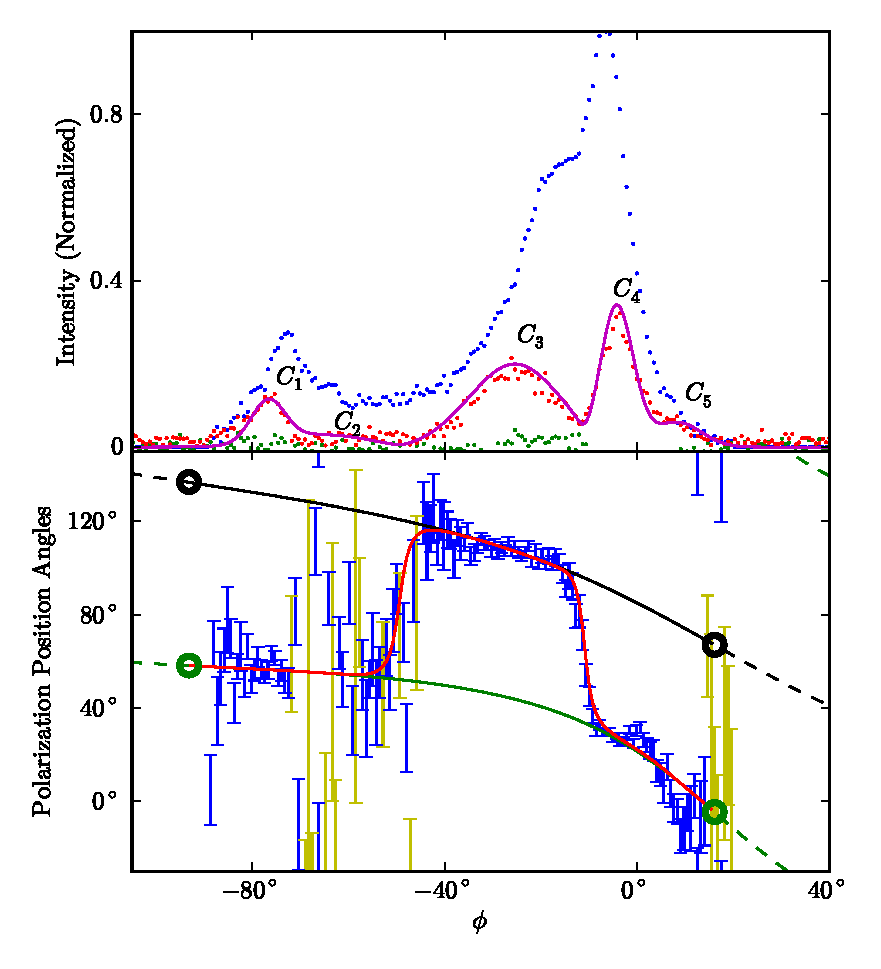
\includegraphics[scale=.8]{chapters/applicationOfNumericalModel/figures/intAndPAJ0023alpha59zeta119.eps}
\caption[Intensity and polarization data for PSR J0023$+$0923 overlaid with model]{\label{fig:PlotJ0023intPA}
In the upper panel, blue points are total radio intensity data at 1.646 GHz, red points are linear polarization intensity data
and green points are circular polarization intensity data for PSR J0023$+$0923.  The solid magenta line in the upper panel is
the model linear intensity used in fitting.  In the bottom panel, blue error bars are polarization position angles
used in the fit and yellow error bars are polarization position angles excluded by error bar cuts (but not 
excluded by phase cuts).  The model polarization comes from
a fit with (unreduced) $\chi^2=332$ and parameters $\alpha=59^{\circ}$ and $\zeta=119^{\circ}$.  The green solid line is the polarization for
a model with $R_{1}=0.77R_{\rm{LC}}$ and the black solid line is the polarization for 
a model with $R_{2}=0.38R_{\rm{LC}}$.  The red solid line is the model
polarization of the two altitudes weighted by the model intensity. Empty circles mark the limiting phase of emission from
open field lines with $\rho_{\rm{ypt}}=1R_{\rm{LC}}$. A phase of zero is the point
of closest encounter to the magnetic axis in the model.
}
\end{center}
\end{figure}


\begin{figure}[t!!]
\begin{center}
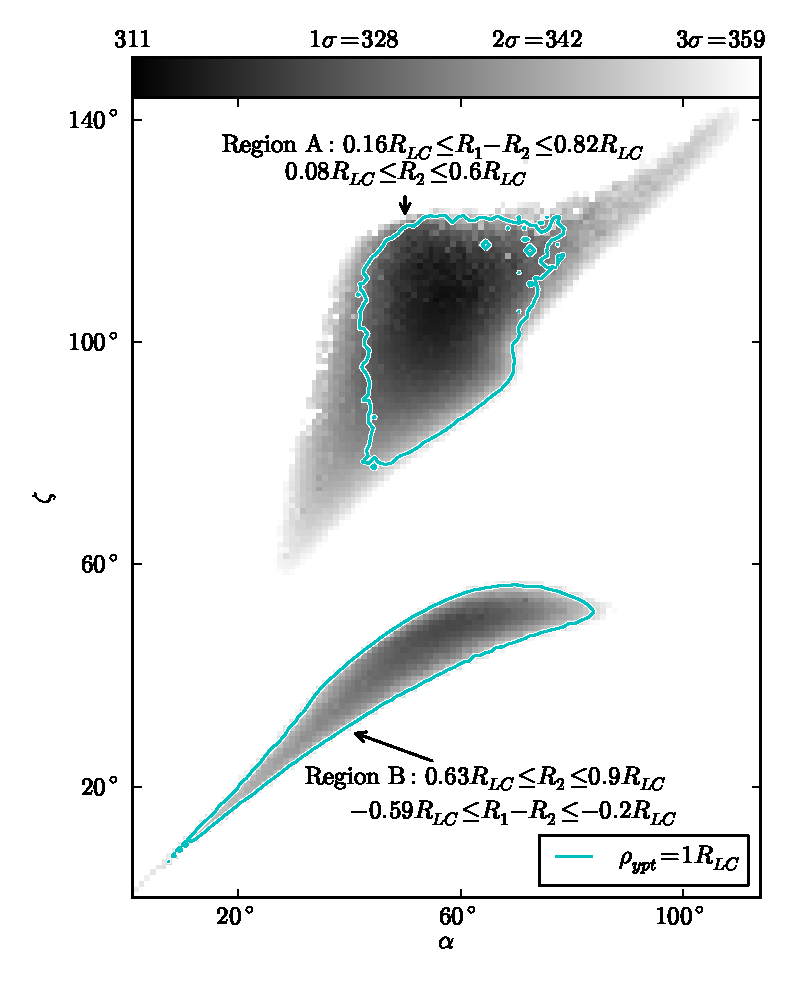
\includegraphics[scale=.8]{chapters/applicationOfNumericalModel/figures/J0023+0923MapWyptRhoCut.eps}
\caption[Map of (unreduced) $\chi^{2}$ for PSR J0023$+$0923 in the $\alpha$--$\zeta$ plane]{\label{fig:J0023Map}
Map of (unreduced) $\chi^{2}$ for PSR J0023$+$0923 in the $\alpha$--$\zeta$ plane.  Cyan contours mark $3\sigma$ from $\chi^2_{\rm{min}}$ 
for fits with $\rho_{\rm{ypt}}=1R_{\rm{LC}}$.  This contour contains the lowest values of $\chi^2$.  The two
regions of statistically acceptable fits have drastically different fit parameters.
}
\end{center}
\end{figure}


PSR J0023$+$0923 is a \textit{Fermi} millisecond pulsar with $P=3.05$ ms.  Figure~\ref{fig:PlotJ0023intPA}
shows the radio pulse profile and the polarization position angles at 1.646 GHz.
The polarization sweep cannot be explained well using the RVM because of
sharp curvature between intensity components $C_2$ and $C_3$ 
and between components $C_3$ and $C_4$.  
The RVM with an orthogonal mode jump between these components
produces more reasonable fits as reported in Table~\ref{tb:fitJ0023}.
This fit is unsatisfying because the jump is closer to $\sim 60^\circ$ rather
than $90^\circ$.  Fitting with an orthogonal mode jump plus two 
altitudes (one altitude, $R_{1}$, assigned to $C_1$, $C_2$, $C_4$, and $C_5$
and a second altitude, $R_{2}$, assigned to $C_3$) gives a fit 
with significantly smaller $\chi^2_{\rm{min}}$ 
(unreduced $\chi^2_{\rm{min}}=313$ versus unreduced $\chi^2_{\rm{min}}=1053$). 
By including two physically motivated
parameters (the two altitudes), the $\chi^2_{\rm{min}}$ is decreased by a factor of three.
The $F$-test between the RVM and the two-altitude model gives $F=149.12$, $\rm{DOF}_1=2$, and $\rm{DOF}_2=125$. 
The $F$ statistic is defined as 
\begin{equation}
F=\frac{\frac{\chi^2_1-\chi^2_2}{\rm{DOF}_1}}{\frac{\chi^2_2}{\rm{DOF}_2}}
\end{equation}
where $\chi^2_2$ is the $\chi^2$ value for the model with the extra model
parameters compared to the model that yields $\chi^2_1$, $\rm{DOF}_1$ 
is the number of extra parameters, and $\rm{DOF}_2$ is
the $\rm{DOF}$ for the model with the extra parameters.
The probability of
exceeding this $F$ is $\rm{Prob}\sim 0$.  This pulsar is an excellent
example of how modeling with multiple altitudes can greatly improve $\chi^2_{\rm{min}}$ compared to the RVM.
It is an example of how multiple altitudes can easily explain a non-$90^\circ$ orthogonal mode jumps since
components of emission with different altitudes allow
for these non-$90^\circ$ mode jumps.
Figure~\ref{fig:PlotJ0023intPA} shows the polarization position angle and intensity data
overlaid with the best fit two altitudes plus the orthogonal mode jump model.


Further confirmation that this mode jump is between components from different
altitudes in the magnetosphere comes from the curvature direction of the polarization position 
angle sweep between adjacent modes.
The polarization sweep direction between components $C_3$ and $C_4$ is in the 
same direction as both the individual unweighted model curves (solid black and red lines).
Such a direction of curvature is impossible for a mode jump between equal altitudes as
discussed in Section~\ref{sec:MAISOM}.  Also, such a direction of curvature is impossible
in the RVM model which partially accounts for the poor fit.


Satisfactory fits exist for both $\rho_{\rm{ypt}}= 1 R_{\rm{LC}}$ and $\rho_{\rm{ypt}}<R_{\rm{LC}}$.
Figure~\ref{fig:J0023Map} is the (unreduced) $\chi^{2}$ map in the $\alpha$--$\zeta$ plane and
the thin cyan contour represents the allowable area up to $3\sigma$ from $\chi^{2}_{\rm{min}}$ in
which the emission comes only from the formal open field line region of the magnetic pole 
as defined by $\rho_{\rm{ypt}}=1R_{\rm{LC}}$.
The minimum $\chi^2$ region is well within the $\rho_{\rm{ypt}}=1R_{\rm{LC}}$ region as seen from Figure~\ref{fig:J0023Map}.
Also Figure~\ref{fig:PlotJ0023intPA} shows a polarization position angle model that 
emits over the entire phase of emission seen in the data where the circles on the plot mark the phase defining
the formal open zone for the two altitudes of emission used in the model.





In the $\alpha$--$\zeta$ plane, two islands of acceptable regions of $\chi^2<3\sigma$ arise as seen in Figure~\ref{fig:J0023Map}.  
Parameters and errors for each of these sections are reported separately in Table~\ref{tb:fitJ0023}.
The distinguishing parameter
between these two regions is $R_{2}$.  For the region between $\zeta=1^{\circ}$ and $\zeta=56^{\circ}$,
$R_{2}=0.63$--$0.90R_{\rm{LC}}$.  For the region between $\zeta=58^{\circ}$ and $\zeta=141^{\circ}$,
$R_{2}=R_{\rm{ns}}=0.08$--$0.61R_{\rm{LC}}$.  
The region between $\zeta=58^{\circ}$ and $\zeta=141^{\circ}$
is more plausible for our model because it favors lower altitudes.  
Additionally, $\Delta R=R_{1}-R_{2}$ for
this region is positive and favors the cone--core model discussed previously (see Table~\ref{tb:fitJ0023}
for values).






\subsection{PSR J1024$-$0719: Kinks with Multiple Altitudes}
\label{sec:J1024}



\begin{table*}[t!!]
\footnotesize
\caption{Fit Parameters for PSR J1024$-$0719}
\tabcolsep=0.05cm
\begin{center}
\def\arraystretch{2}
\scalebox{0.75}{
\begin{tabular}{lccccccccc}
%\scriptsize
\hline
\hline
 &&(Unreduced)&&&&&&&\\
 &DOF&$\chi^{2}_{\rm{min}}$& $\alpha$ ($^\circ$) & $\zeta$ ($^\circ$) & $R_1$ ($R_{\rm{LC}}$)& $R_2$ ($R_{\rm{LC}}$)& $\Delta R$ ($R_{\rm{LC}}$)& $\Delta \rho$ ($R_{\rm{LC}}$)& $\rho_{\rm{ypt}}$ ($R_{\rm{LC}}$)\\
[.3em] \hline  %[-1em]
RVM & 397-4&$  8963 $ & $98 ^{+1(+3)}_{-3(-4)} $ & $87 ^{+1(+2)}_{-2(-2)} $&\ldots &\ldots &\ldots &\ldots &\ldots \\ \hline
Region A 2 Alt &397-6&$  3409 $ & $  112 ^{  + 1(+2)}_{   -1(-3)} $ & $   63 ^{+2(+5)}_{-3(-6)} $ 
& $ 0.90 ^{+0.00(+0.00)}_{-0.02(-0.05)} $ & $ 0.82 ^{+0.00(+0.01)}_{-0.02(-0.05)} $ 
& $ 0.08 ^{+0.01(+0.01)}_{-0.00(-0.01)} $ & $ 0.11 ^{+0.00(+0.01)}_{-0.01(-0.01)} $ & $ 1.00 ^{+0.00(+0.00)}_{-0.02(-0.04)} $ \\ \hline
Region B 2 Alt &397-6&$  3447 $ & $  113 ^{+1(+4)}_{-1(-4)} $ & $  108 ^{+1(+4)}_{-1(-4)} $
& $ 0.22 ^{+0.01(+0.04)}_{-0.03(-0.05)} $ & $ 0.05 ^{+0.00(+0.01)}_{-0.00(-0.00)} $ 
& $ 0.17 ^{+0.01(+0.04)}_{-0.03(-0.05)} $ & $ 0.04 ^{+0.01(+0.08)}_{-0.01(-0.03)} $ & $ 0.24 ^{+0.00(+0.07)}_{-0.02(-0.04)} $ \\ \hline
\end{tabular} }
\tablecomments{Errors reported without (with) parentheses are for $1\sigma$ ($3\sigma$) from $\chi^2_{\rm{min}}$. }
\label{tb:fitJ1024} 
\end{center} 
\end{table*}

\begin{figure}[htbp]
\begin{center}
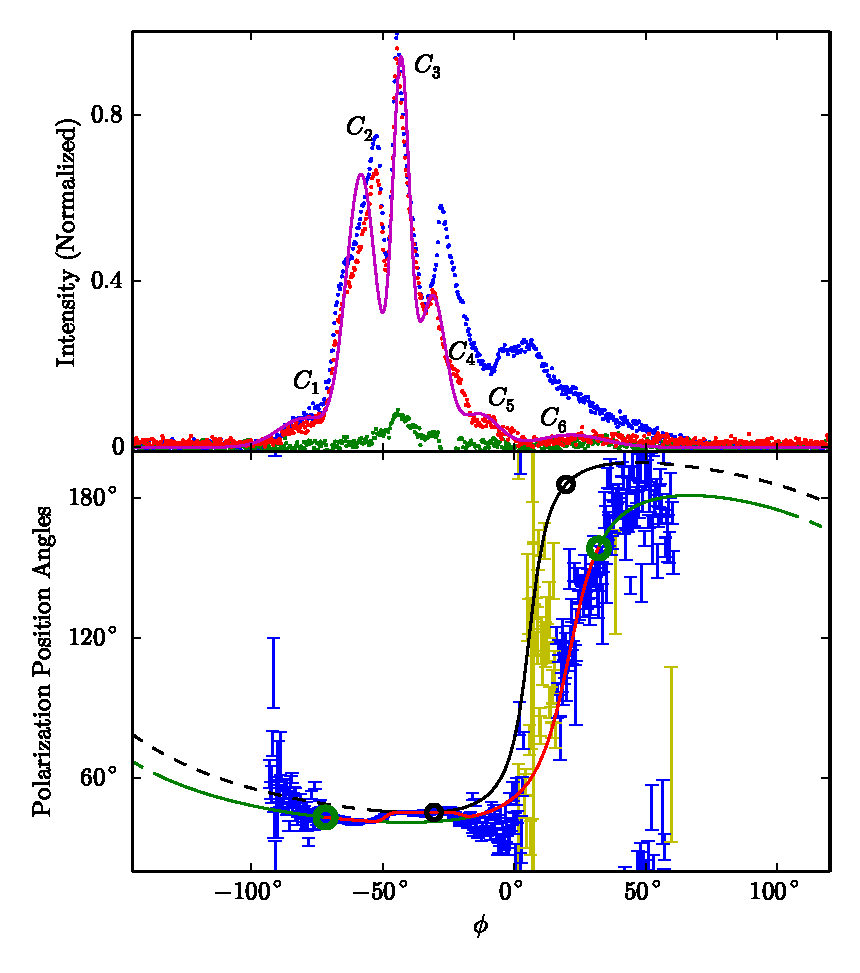
\includegraphics[scale=.8]{chapters/applicationOfNumericalModel/figures/intAndPAJ1024alpha113zeta108.eps}
\caption[Intensity and polarization data for PSR J1024$-$0719 overlaid with model]{\label{fig:PlotJ1024intPA}
In the upper panel, blue points are total radio intensity data for 1.369 GHz, red points are linear polarization intensity data,
and green points are circular polarization intensity data for PSR J1024$-$0719.  The solid magenta line in the upper panel is
the model linear intensity used in fitting.  In the bottom panel, blue error bars are polarization position angles
used in the fit and yellow error bars are polarization position angles excluded by error bar cuts (but not 
excluded by phase cuts).
The model polarization comes from
a fit with (unreduced) $\chi^2=3448$ and parameters $\alpha=113^{\circ}$ and $\zeta=108^{\circ}$.  The green solid line is the polarization for
a model with $R_{1}=0.22R_{\rm{LC}}$ and the black solid line is the polarization for 
a model with $R_{2}=0.05R_{\rm{LC}}$.  The red solid line is the model
polarization of the two altitudes weighted by the model intensity. Empty circles mark the limiting phase of emission from
open field lines with $\rho_{\rm{ypt}}=1R_{\rm{LC}}$.  
Solid lines mark the allowed emission phase for an effective open zone with $\rho_{\rm{ypt}}=0.24R_{\rm{LC}}$ which is
required for the model phase to cover the entire emission phase in the data.
A phase of zero is the point
of closest encounter to the magnetic axis in the model.
}
\end{center}
\end{figure}


\begin{figure}[t!!]
\vskip .5\textheight
\special{psfile=chapters/applicationOfNumericalModel/figures/J1024-0719MapBRhoCut.eps hoffset=72 voffset=-160 vscale=80 hscale=80 angle=0}
\special{psfile=chapters/applicationOfNumericalModel/figures/J1024-0719MapARhoCut.eps hoffset=-140 voffset=-160 vscale=80 hscale=80 angle=0}
\begin{center}
\caption[Map of (unreduced) $\chi^{2}$ for PSR J1024$-$0719 in the $\alpha$--$\zeta$ plane for Regions A and B]{\label{fig:J1024Map}
Map of (unreduced) $\chi^{2}$ for PSR J1024$-$0719 in the $\alpha$--$\zeta$ plane for Regions A and B.
The regions vary drastically from one another in parameters although they are comparable in $\chi^2$.
Both are very restrictive in their respective parameters.  
}
\end{center}
\vskip -0.2truecm
\end{figure}


PSR J1024$-$0719 is another millisecond \textit{Fermi}-detected pulsar ($P=5.162$ ms). 
This pulsar fits reasonably well to the RVM (1.369 GHz data shown in 
Figure~\ref{fig:PlotJ1024intPA}) although certain features 
in the polarization data are highly statistically significant
and unexplained by the RVM.  Most notably, a kink in the polarization occurs in 
the transition from  intensity component $C_2$ to 
$C_3$ and from $C_4$ to $C_5$ (as labeled on Figure~\ref{fig:PlotJ1024intPA}).  
Similar to PSR J0023$+$0923, this jump can be modeled using
multiple altitudes, modeling the kink as the shift in altitude
between the emission components.  The error bars
on this model are fairly small for the fit parameters (Table~\ref{tb:fitJ1024}) 
since a limited number of parameter combinations
make a sweep with this particular polarization difference with two heights.  Additionally, the data contains
the polarization at the point of closest encounter to the magnetic axis (the fastest change in the sweep) which
also greatly constrains the fitting parameters.
Overall, this pulsar is another excellent example of how using multiple altitudes can explain 
features not found in the RVM.

Similar to PSR J0023$+$0923, two regions arise in the $\alpha$--$\zeta$ plane of the (unreduced) $\chi^2$ map
(see Figure~\ref{fig:J1024Map}) that are statistically acceptable.  For the 
two regions, the altitudes are significantly different and are reported separately in Table~\ref{tb:fitJ1024}.

In Region A, the $\rho_{\rm{ypt}}$ needs to be 
$ 0.22 R_{\rm{LC}} \leq \rho_{\rm{ypt}} \leq 0.34 R_{\rm{LC}}$ in order to account for the full 
phase of the emission and remain within $3\sigma$ of $\chi^2_{\rm{min}}$. 
Figure~\ref{fig:PlotJ1024intPA} displays the model polarization sweep from this region.
The green and black circles represent the limiting phase 
of emission defined by the formal cap with $\rho_{\rm{ypt}}=1R_{\rm{LC}}$.
The solid lines mark the effective open zone emission for $\rho_{\rm{ypt}}=0.24R_{\rm{LC}}$.
Both sets of circles are well within the limiting phase of emission seen in the data.
For most of the models within $3\sigma$ of $\chi^2_{\rm{min}}$, 
the emission phase of the outer altitude ($R_1$ represented 
by the green line in Figure~\ref{fig:PlotJ1024intPA}) 
controls the location of $\rho_{\rm{ypt}}$.
For Region A, $R_{1}=0.14$--$0.26R_{\rm{LC}}$, $R_{2}=0.05$--$0.06R_{\rm{LC}}$. 
The outer emission altitude, $R_{1}$, is typically larger than the inner emission altitude, $R_{2}$, which is
consistent with a cone--core model similar to the two fit altitude parameters for the polarization
position data from PSR J0023$+$0923 .

For Region B, the $\rho_{\rm{ypt}}$ is much higher than that in Region A but likewise so are $R_{1}$ and $R_{2}$.
Approximately $\rho_{\rm{ypt}}=0.96$--$1.0R_{\rm{LC}}$, 
$R_{1}=0.85$--$0.9R_{\rm{LC}}$, $R_{2}=0.77$--$0.83R_{\rm{LC}}$.
Although $\rho_{\rm{ypt}}$ is much larger in Region B than in Region A, the altitude of 
emission is also close to $R_{\rm{LC}}$ resulting in a $\Delta \rho=\rho_{\rm{ypt}}-\rho_{\rm{max}}$
(the
difference between the y-point cylindrical distance needed to open up the field lines
to the appropriate amount to accommodate the emission phase in the data and
the maximum cylindrical distance of the emission within this phase)
similar to that of
Region A.  Additionally, $\Delta \rho$
is relatively
small (see Table~\ref{tb:fitJ1024}).  This is problematic because we expect emission 
this close to the light cylinder to resemble a force-free model and to be dictated
by physics that we do not include in the vacuum model.
To explain the phase of emission seen in the data using this model, one must either push the 
altitude up to extreme heights or accept $\rho_{\rm{ypt}}$ much smaller than $1R_{\rm{LC}}$.

PSR J1024$-$0719 is modeled with two altitudes, one altitude component inside the other
in terms of phase, making it a good candidate for the cone--core model.  The parameter
$\Delta R=R_1-R_2$ (where $R_1$ is the altitude associated with component $C_1$, $C_2$, $C_5$, and $C_6$ and
$R_2$ is the altitude associated with $C_3$ and $C_4$) should be positive in the
case of a cone--core model.  Table~\ref{tb:fitJ1024} shows this value to be positive
for both Regions A and B.  
Further, to $3\sigma$, these values are positive and radio modeling of PSR J1024$-$0719 polarization
is consistent with the cone--core model.

For the RVM (unreduced) $\chi^2_{\rm{min}}=8963$ 
and for the two-altitude model (unreduced) $\chi^2_{\rm{min}}=3408$. By including two physically motivated 
parameters, the $\chi^2_{\rm{min}}$ is decreased by a factor of three.  
The $F$-test between the RVM and the two-altitude model gives $F=318.66$, DOF$_1=2$, and DOF$_2=391$. The probability of
exceeding this $F$ is Prob$\sim 0$.  By these statistical measures, a two-altitude model is clearly
better than the RVM.



\subsection{PSR J1057$-$5226: Y-Point and Finite Altitude}
\label{sec:J1057}

\begin{table*}[t!!]
%\footnotesize
\small
\tabcolsep=0.05cm
\caption{Fit Parameters for PSR J1057$-$5226} 
\begin{center}
\def\arraystretch{2}
\scalebox{0.75}{
\begin{tabular}{lccccccccc}
\hline
\hline
 &&(Unreduced)&&&&&&&\\
& DOF&$\chi^2_{\rm{min}}$ & $\alpha$ ($^\circ$) & $\zeta$ ($^\circ$) & $R_1$ ($R_{\rm{LC}}$)& $R_2$ ($R_{\rm{LC}}$)& $\Delta \rho$ ($R_{\rm{LC}}$)& $\rho_{\rm{max}}$ ($R_{\rm{LC}}$)& $\rho_{\rm{ypt}}$ ($R_{\rm{LC}}$)\\ 
[.3em]\hline 

RVM & 166-4&$   325 $ & $   77 ^{     +0(+1)}_{   -1(-1)} $ & $   70 ^{     +0(+0)}_{    -0(-0)} $  &\ldots &\ldots &\ldots &\ldots &\ldots \\ \hline

1 Alt & 166-5&$   282 $ & $   76 ^{+2(+2)}_{0(-1)} $ & $   64 ^{+5(+5)}_{-34(-35)} $  & $ 0.19 ^{+0.43(+0.46)}_{-0.12(-0.13)} $ &\ldots  &\ldots &\ldots &\ldots\\ \hline

2 Alt & 166-6&$   281 $ & $   69 ^{+14(+26)}_{-4(-9)} $ & $   64 ^{+5(+6)}_{-37(-39)} $ 
& $ 0.12 ^{+0.72(+0.72)}_{-0.06(-0.12)} $ & $ 0.31 ^{+0.59(+0.59)}_{-0.29(-0.31)} $ 
& $ 0.15 ^{+0.32(+0.40)}_{-0.15(-0.15)} $ & $ 0.31 ^{+0.36(+0.52)}_{-0.25(-0.28)} $ & $ 0.46 ^{+0.54(+0.54)}_{-0.40(-0.40)} $ \\ \hline

\end{tabular} }
\tablecomments{Errors reported without (with) parentheses are for $1\sigma$ ($3\sigma$) from $\chi^2_{\rm{min}}$. }
\label{tb:fitJ1057}
\end{center} 
\end{table*}



\begin{figure}[htbp]
\begin{center}
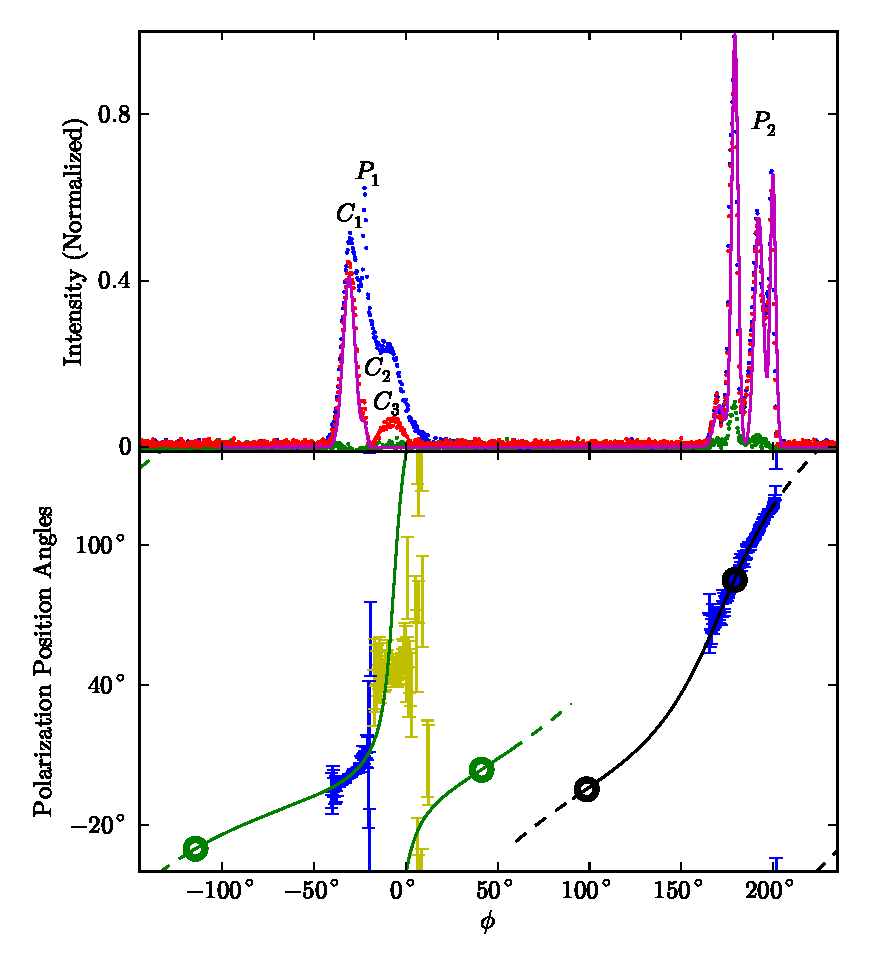
\includegraphics[scale=.8]{chapters/applicationOfNumericalModel/figures/intAndPAJ1057alpha77zeta30.eps}
\caption[Intensity and polarization data for PSR J1057$-$5226 overlaid with model]{\label{fig:PlotJ1057intPA}
In the upper panel, blue points are total radio intensity data for 1.5 GHz, red points are linear polarization intensity data,
and green points are circular polarization intensity data for PSR J1057$-$5226.  The solid magenta line in the upper panel is
the model linear intensity used in fitting.  In the bottom panel, blue error bars are polarization position angles
used in the fit and yellow error bars are polarization position angles excluded from the 
fit because of phase cuts (see text).
The model polarization comes from
a fit with (unreduced) $\chi^2=289$ and parameters $\alpha=77^{\circ}$ and $\zeta=30^{\circ}$.  The green solid line is the polarization for
a model with $R_{1}=0.58R_{\rm{LC}}$ and the black solid line is the polarization for 
a model with $R_{2}=0.63R_{\rm{LC}}$.
Empty circles mark the limiting phase of emission from
open field lines with $\rho_{\rm{ypt}}=1R_{\rm{LC}}$.
Solid lines mark allowed emission phase for an effective open zone with
$\rho_{\rm{ypt}}=0.71R_{\rm{LC}}$ ($\Delta\rho=0.49R_{\rm{LC}}$) which is
required for the model phase to cover the entire emission phase in the data.
A phase of zero is the point
of closest encounter to the magnetic axis in the model.
}
\end{center}
\end{figure}


\begin{figure}[t!!]
\begin{center}
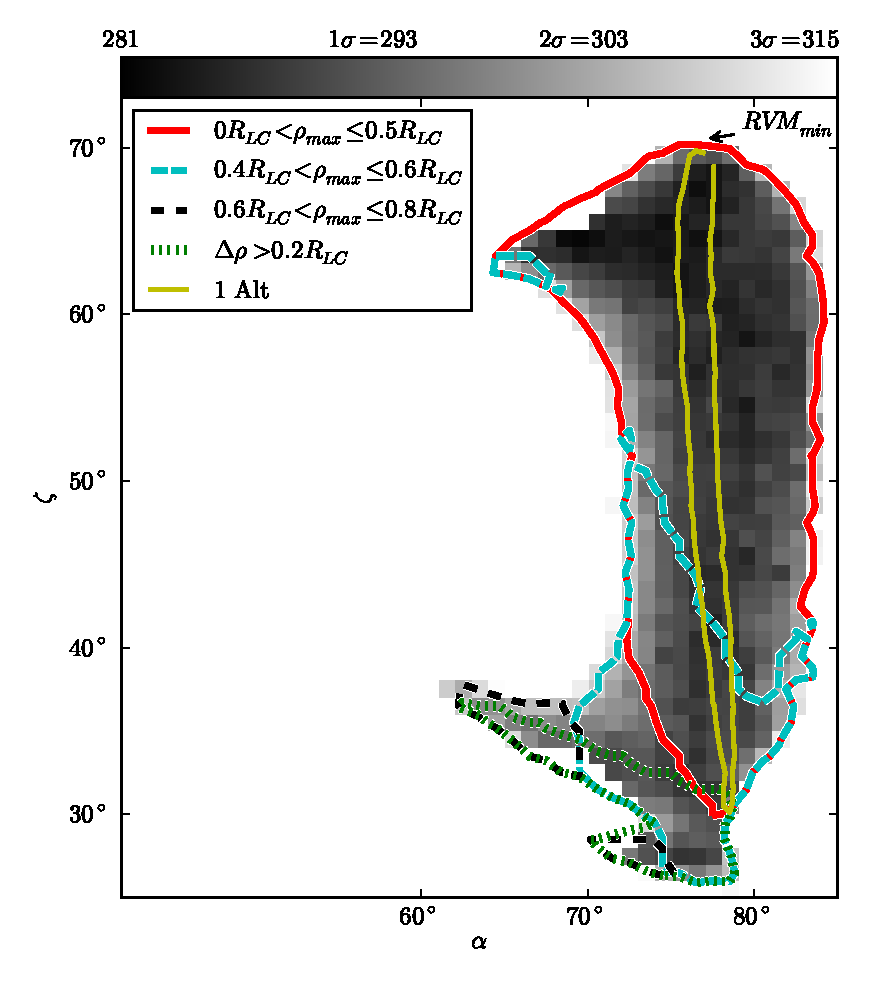
\includegraphics[scale=.8]{chapters/applicationOfNumericalModel/figures/J1057-5226MapTotRhoCut.eps}
\caption[Map of (unreduced) $\chi^{2}$ for PSR J1057$-$5226 in the $\alpha$--$\zeta$ plane]{\label{fig:J1057Map}
Map of (unreduced) $\chi^{2}$ for PSR J1057$-$5226 in the $\alpha$--$\zeta$ plane with $3\sigma$ contours for sets of $\rho_{\rm{max}}$ ranges, 
the single-altitude model fit,
and $\Delta\rho>0.2R_{\rm{LC}}$.  The best fit for the RVM is also indicated on the map.  The best fit using the RVM
is quite different from the best fit using finite altitude and restrictions from the phase of emission
seen in the data ($\Delta\rho>0.2R_{\rm{LC}}$).
}
\end{center}
\end{figure}


PSR J1057$-$5226 is a relatively young pulsar ($P=197.11$ ms) that has had its radio polarization
position angle sweep fit in the literature with the RVM \citep{weltevrede2009mapping}.  
Here we fit the latest polarization data for PSR J1057$-$5226 at 1.369 GHz with 
the RVM plus our own finite-altitude model.  Polarization and intensity 
data for PSR J1057$-$5226 is plotted in 
Figure~\ref{fig:PlotJ1057intPA}.  First note that we are unable
to explain the polarization position angles associated
with $C_{3}$ as labeled in Figure~\ref{fig:PlotJ1057intPA}
with either the RVM or our current model.
This portion of the polarization sweep had not appeared in the previous 
RVM fitting papers due to poor signal-to-noise.  Although we will not
attempt to explain this component here, we hope to explore modifications to 
our current model that will explain this component in future work.

Ignoring the polarization position angles associated
with $C_{3}$ for the moment, unlike PSR J0023$+$0923 and PSR J1024$-$0719,
PSR J1057$-$5226 does not have any compelling features to indicate mode jumps or
multiple altitudes.  The $\chi^2_{\rm{min}}$ for the RVM even gives a reasonable fit for the 
number of degrees of freedom (DOF, Table~\ref{tb:fitJ1024}).  Even so, 
by fitting to a finite altitude and 
finite multiple altitudes, we can significantly decrease the 
$\chi^2_{\rm{min}}$ and open the parameter space.  Further, \citet{weltevrede2009mapping}
were forced to conclude that emission comes from outside the
formal open zone cap due to the large emission phase of PSR J1057$-$5226.
Here we seek a more physical model using a finite altitude and $\rho_{\rm{ypt}}<R_{\rm{LC}}$.



We can model the data with $\rho_{\rm{ypt}}=1R_{\rm{LC}}$ within 
$1\sigma$ of $\chi^2_{\rm{min}}$ but this 
requires pushing the model to the highest allowed altitudes.  
On the other hand, low altitudes
are also permitted but require low $\rho_{\rm{ypt}}$ in 
order for the models to emit in the phase observed
in the data.  The true fit likely lies somewhere between the extremes.  A strong correlation 
exists between $\alpha$, $\zeta$, $R_{1}$, and $R_{2}$ such 
that if one has an estimated range for $R_{1}$ or $R_{2}$, the acceptable $\alpha$--$\zeta$ 
models would be significantly decreased. 

Red, cyan, and black contours on Figure~\ref{fig:J1057Map} are $3\sigma$ contours
from $\chi^2_{\rm{min}}$ of different ranges of $\rho_{\rm{max}}$, the maximum cylindrical 
distance of the emission within the emission phase for the model.  These contours exemplify
the correlation between altitude and $\alpha$--$\zeta$ pairs in a single parameter.  Further, fits with smaller
$\rho_{\rm{max}}$ are more physically likely but so is larger $\Delta \rho$ such as 
$\Delta \rho> 0.2 R_{\rm{LC}}$ ($3\sigma$ dashed green contours
on Figure~\ref{fig:J1057Map}).  As such, one might expect the most physically plausible
fits to fall within the green and cyan contours.

The yellow contour is the $3\sigma$ contour from $\chi^2_{\rm{min}}$ 
of a single-altitude model.  
Going from one altitude to two altitudes does not greatly improve $\chi^2_{\rm{min}}$.
Adding the additional parameter does allow for a wider variety of geometric
configurations ($\alpha$ and $\zeta$) which could be of importance when comparing
to multi-wavelength results.


For the RVM (unreduced) $\chi^2_{\rm{min}}=325$ and for the 
two-altitude model (unreduced) $\chi^2_{\rm{min}}=281$
(see Table~\ref{tb:fitJ1057}).
The $F$-test between the RVM and the two-altitude 
model gives $F=12.50$, DOF$_1=2$, and DOF$_2=160$. The probability of
exceeding this $F$ is $P=8.78\e{-6}$. Comparing the RVM 
to the single-altitude model ($\chi^2_{\rm{min}}=282$), the
probability of exceeding $F=24.55$ is $\rm{Prob}=1.82\e{-6}$.  
Comparing the single-altitude model to the two-altitude model, the
probability of exceeding $F=0.57$ is $\rm{Prob}=4.52\e{-1}$.



\subsection{PSR J1744$-$1134: Multiple Altitudes with Single Versus Double Pole}
\label{sec:J1744}

\begin{table*}[t!!]
\small
\tabcolsep=0.1cm
\caption{Fit Parameters for PSR J1744$-$1134}
\begin{center}
\def\arraystretch{2}
\scalebox{0.74}{
\begin{tabular}{lcccccccc}
\hline
\hline
&&(Unreduced)&&&&&\\
& DOF&$\chi^2_{\rm{min}}$ & $\alpha$ ($^\circ$) & $\zeta$ ($^\circ$) & $R_1$ ($R_{\rm{LC}}$)& $R_2$ ($R_{\rm{LC}}$)& $\Delta \rho$ ($R_{\rm{LC}}$)& $\rho_{\rm{ypt}}$ ($R_{\rm{LC}}$)\\ 
[.3em]\hline

RVM & 209-4&$   355 $ & $ 74 ^{+0(+1)}_{-2(-4)} $ & $97 ^{+0(+1)}_{-2(-3)} $ &  \ldots&\ldots &\ldots&\ldots \\ \hline

2 Alt no jump & 209-6&$   311 $ & $   76 ^{+2(+6)}_{-11(-15)} $ & $   60 ^{8(+84)}_{-18(-26)} $ 
& $ 0.68 ^{+0.09(+0.18)}_{-0.12(-0.62)} $ & $ 0.70 ^{+0.20(+0.20)}_{-0.03(-0.64)} $ 
& $ 0.06 ^{+0.00(+0.33)}_{-0.04(-0.06)} $ & $ 0.73 ^{+0.19(+0.27)}_{-0.03(-0.06)} $ \\ \hline

2 Alt jump & 209-6&$   314 $ & $   92 ^{+2(+4)}_{-53(-70)} $ & $57 ^{+76(+79)}_{-8(-32)} $ 
& $ 0.87 ^{+0.03(+0.03)}_{-0.76(-0.81)} $ & $ 0.88 ^{+0.02(+0.02)}_{-0.24(-0.44)} $ 
& $ 0.05 ^{+0.24(+0.27)}_{-0.05(-0.05)} $ & $ 0.81 ^{+0.19(+0.19)}_{-0.11(-0.37)} $ \\ \hline

1 Alt single pole & 209-5& $310$ & $66 ^{+5(+15)}_{-4(-7)}$ & $85 ^{+3(+35)}_{-36(-39)}$  
& $0.65 ^{+0.07(+0.20)}_{-0.27(-0.54)} $ & \ldots
& $ 0.36 ^{+0.09(+0.12)}_{-0.35(-0.47)} $ & $ 0.99 ^{+0.01(+0.01)}_{-0.50(-0.86)} $ \\ \hline

2 Alt single pole & 209-6& $309 $ & $66 ^{+11(+17)}_{-22(-36)} $ & $85 ^{+24(+32)}_{-53(-60)} $ 
& $ 0.65 ^{+0.14(+0.25)}_{-0.55(-0.59)} $ & $ 0.59 ^{+0.31(+0.31)}_{-0.23(-0.52)} $ 
& $ 0.37 ^{+0.19(+0.30)}_{-0.37(-0.37)} $ & $ 1.00 ^{0.00(+0.00)}_{-0.56(-0.93)} $ \\ \hline


\end{tabular} }
\tablecomments{Errors reported without (with) parentheses are for $1\sigma$ ($3\sigma$) from $\chi^2_{\rm{min}}$. }
\label{tb:fitJ1744-1134} 
\end{center} 
\end{table*}



\begin{figure*}[t!!]
\vskip .5\textheight
\special{psfile=chapters/applicationOfNumericalModel/figures/intAndPAJ1744alpha82zeta39.eps hoffset=-110 voffset=-80 vscale=60 hscale=60}
\special{psfile=chapters/applicationOfNumericalModel/figures/intAndPAJ1744alpha66zeta85.eps hoffset=155 voffset=-90 vscale=60 hscale=60}
\begin{center}
\caption[Intensity and polarization data for PSR J1744$-$1134 overlaid with model]{\label{fig:PlotJ1744intPA}
In the upper panels, blue points are total radio intensity data for 1.369 GHz, red points are linear polarization intensity data,
and green points are circular polarization intensity data for PSR J1744$-$1134.  The solid magenta line in the upper panels is
the model linear intensity used in fitting.  In the bottom panels, blue error bars are polarization position angles
used in the fit.
For panel (A), the model polarization comes from a double magnetic pole model with (unreduced) $\chi^2=342$, $\alpha=82^{\circ}$, and
$\zeta=39^{\circ}$.  The green line is the polarization for
a model with $R_{1}=0.78R_{\rm{LC}}$ and the black line is the polarization for 
a model with $R_{2}=0.72R_{\rm{LC}}$.
The emission phase from the data for these model parameters 
requires $\rho_{\rm{ypt}}=0.96R_{\rm{LC}}$ as marked on the plot with the solid lines.
For panel (B), the model polarization comes from a single magnetic pole model with (unreduced) $\chi^2=317$, $\alpha=66^{\circ}$, and 
$\zeta=85^{\circ}$.  The green solid line is the polarization for
a model with $R_{1}=0.65R_{\rm{LC}}$ and the black solid line is the polarization for 
a model with $R_{2}=0.59R_{\rm{LC}}$.  
The emission phase from the data is covered with $\rho_{\rm{ypt}}=1R_{\rm{LC}}$ for these model parameters.
Empty circles mark the limiting phase of emission from
open field lines with $\rho_{\rm{ypt}}=1R_{\rm{LC}}$.
A phase of zero is the point
of closest encounter to the magnetic axis in the model.
}
\end{center}
\vskip -0.2truecm
\end{figure*}




\begin{figure}[t!!]
\begin{center}
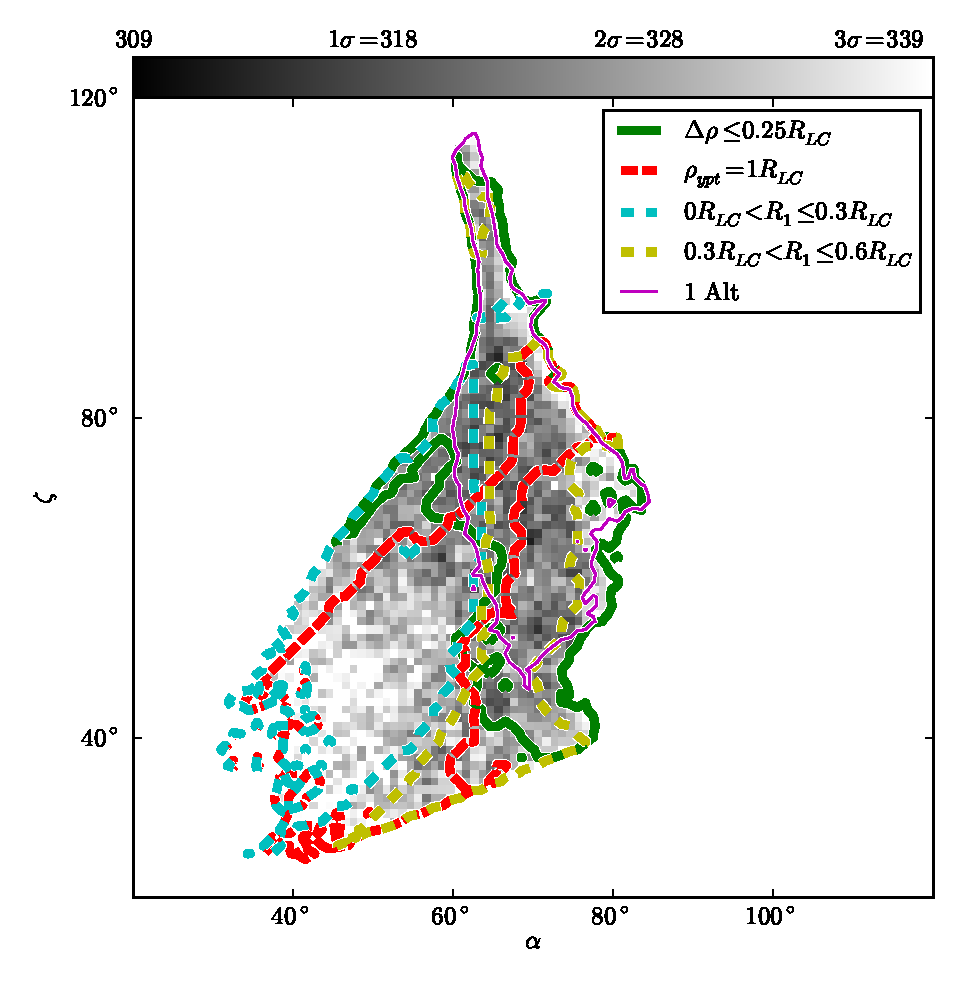
\includegraphics[scale=.8]{chapters/applicationOfNumericalModel/figures/J1744-1134MapNoJumpSPtotRhoCut.eps}
\caption[Map of (unreduced) $\chi^{2}$ for PSR J1744$-$1134 in the $\alpha$--$\zeta$ plane]{\label{fig:J1744-1134MapNoJumpSP}
Map of (unreduced) $\chi^{2}$ for PSR J1744$-$1134 in the $\alpha$--$\zeta$ plane for a single magnetic pole model with $3\sigma$ 
contours for two $R_{1}$ ranges to show correlation between $\alpha$, $\zeta$, and altitude for
$\Delta\rho\leq 0.25R_{\rm{LC}}$ (the more approximate models) and $\rho_{\rm{ypt}}=1R_{\rm{LC}}$
(the less approximate models), and for the single-altitude model which lies mostly 
in the physically inaccurate contour of $\Delta\rho\leq 0.25R_{\rm{LC}}$ and therefore argues for a 
two-altitude model.
}
\end{center}
\end{figure}


PSR J1744$-$1134 is yet another millisecond pulsar detected in $\gamma$-rays 
by \textit{Fermi}.  Similar to PSR J1057$-$5226, 
the polarization of PSR J1744$-$1134 fits well to the RVM.  
But even with the consideration that the star surface is 
$\sim 0.06R_{\rm{LC}}$ based on period, the emission zone
of a vacuum dipole model with emission from both poles is not large enough to accommodate 
the range of the emission in phase seen in the data. 
In the vast majority of fits, the cylindrical distance between
the edge of the open zone required and the maximum cylindrical emission
point ($\Delta \rho$) is smaller than $0.2R_{\rm{LC}}$.  We considered a
two-pole model with and without an orthogonal mode jump between the polarization
position angles associated with $P_1$ and $P_2$ as labeled on Figure~\ref{fig:PlotJ1744intPA}.
Results for the fits are reported in Table~\ref{tb:fitJ1744-1134}.  

The peaks, $P_1$ and $P_2$, are separated by $\sim 103^{\circ}$--$134^{\circ}$; thus another possibility is that the emission
is not from two magnetic poles but a single broad pulse.  Interestingly, with this assumption,
models exist within the $1\sigma$ multidimensional contour with $\rho_{\rm{ypt}}=1R_{\rm{LC}}$.
Figure~\ref{fig:J1744-1134MapNoJumpSP} shows the $\alpha$--$\zeta$ maps of (unreduced) $\chi^2$
for the single broad pulse model.  The red contour shows the $3\sigma$ range with the 
assumption that $\rho_{\rm{ypt}}=1R_{\rm{LC}}$. Additionally, the green contour is the $3\sigma$
contour with a $\Delta \rho \leq 0.25R_{\rm{LC}}$ cut and the thin magenta line is the $3\sigma$
contour if $R_1=R_2$; these two contours strongly overlap which makes us slightly favor models
where $R_1\neq R_2$.  Quite a range of altitudes falls 
within the $3\sigma$ contours and there is
a strong correlation between $R_1$ and $\alpha$ and $\zeta$.  We also plotted two rough ranges
of $R_1$ on the $\alpha$--$\zeta$ map to illustrate this correlation.
Overall, the polarization position angles associated 
with $P_2$ are very noisy, which translates
into noisy $\chi^2$ surfaces.  To decrease this noise, 
we applied a $0\degr5$ Gaussian smoothing kernel
to the map and contours.  Additionally, Figure~\ref{fig:PlotJ1744intPA},
panel (B) shows the polarization sweep derived from a
single magnetic pole model with $\alpha=66^\circ$ and $\zeta=85^\circ$.

For single-pole and double-pole models, fit parameters and errors are reported in Table~\ref{tb:fitJ1744-1134}.
Overall, adding a finite altitude, whether using 
a single-pole or two-pole model, significantly decreases the $\chi^2_{\rm{min}}$
which can be shown statistically using an $F$-test.  
The (unreduced) $\chi^2_{\rm{min}}=355$ for the RVM and $\rm{DOF}_1=2$, and $\rm{DOF}_2=203$
for the $F$-test.  For the single magnetic pole emission 
(unreduced $\chi^2_{\rm{min}}=309$), the probability of exceeding the resulting $F$ is $P=7.63\e{-7}$;
for the two magnetic pole model without 
an orthogonal mode jump (unreduced $\chi^2_{\rm{min}}=311$), 
the probability of exceeding the resulting $F$ is 
$P=1.47\e{-6}$; for the two magnetic pole model 
with an orthogonal mode jump (unreduced $\chi^2_{\rm{min}}=314$), the probability of 
exceeding the resulting $F$ is $P=3.89\e{-6}$.


%\vskip 1.0truecm
\subsection{PSR J1420$-$6048: Multiple Altitudes and Interstellar Scattering}
\label{sec:J1420}

\begin{figure*}[t!!]
\vskip .5\textheight
\special{psfile=chapters/applicationOfNumericalModel/figures/intAndPAJ1420alpha120zeta150T0.eps hoffset=-110 voffset=-90 vscale=60 hscale=60}
\special{psfile=chapters/applicationOfNumericalModel/figures/intAndPAJ1420alpha120zeta150.eps hoffset=150 voffset=-90 vscale=60 hscale=60}
\begin{center}
\caption[Intensity and polarization data for PSR J1420$-$6048 overlaid with model]{\label{fig:PlotJ1420intPA}
In the upper panel, blue points are total radio intensity data, red points are linear polarization intensity data,
and green points are circular polarization intensity data for PSR J1420$-$6048.  The solid magenta line in the upper panel is
the model linear intensity used in fitting.  In the bottom panel, blue error bars are polarization position angles
used in the fit.
The model polarization comes from
a fit with (unreduced) $\chi^2=435$ (joint fit with data from both 10 cm and 20 cm) 
and parameters $\alpha=120^{\circ}$, $\zeta=150^{\circ}$, and $R_{1}=0.53R_{\rm{LC}}$ weighted by the model intensity.
Panel (A) shows the 10 cm intensity and polarization position angle data and the model with scattering time $\tau\sim0$ ms.
Panel (B) is the 20 cm intensity and polarization position angle data and the model with scattering time $\tau=1.3$ ms.
The $\rho_{\rm{ypt}}<1R_{\rm{LC}}$ constraints lie beyond the phase plotted.
A phase of zero is the point
of closest encounter to the magnetic axis in the model.
}
\end{center}
\vskip -0.2truecm
\end{figure*}

\begin{figure}[t!!]
\begin{center}
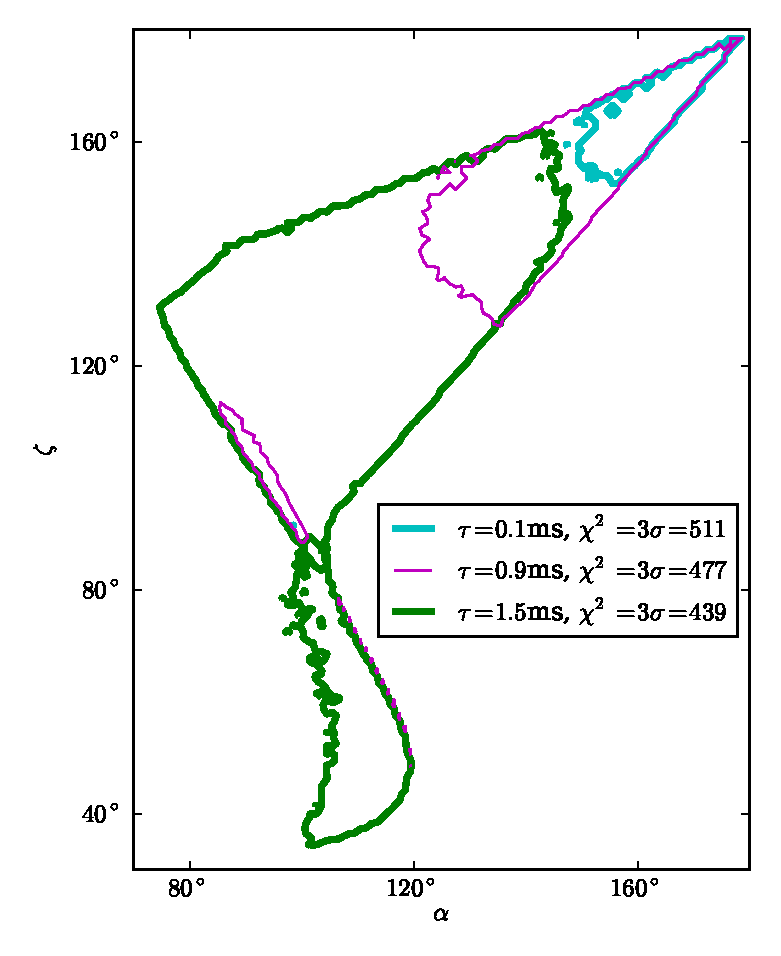
\includegraphics[scale=.8]{chapters/applicationOfNumericalModel/figures/J1420ContoursMap.eps}
\caption[Contours of the joint (unreduced) $\chi^2$ set to $3\sigma$ in the $\alpha$--$\zeta$ plane for modeling of
the polarization data in 10 cm and 20 cm of PSR J1420$-$6048]{\label{fig:diffTau}
Contours of the joint (unreduced) $\chi^2$ set to $3\sigma$ in the $\alpha$--$\zeta$ plane for modeling of 
the polarization data in 10 cm and 20 cm of PSR J1420$-$6048.  
Different colors represent fits to different $\tau$, scattering time.  
Increasing scattering time widens the acceptable fit parameters, decreases the acceptable $\alpha$ 
values, and decreases $\chi^2_{\rm{min}}$.
}
\end{center}
\end{figure}

\begin{figure}[t!!]
\begin{center}
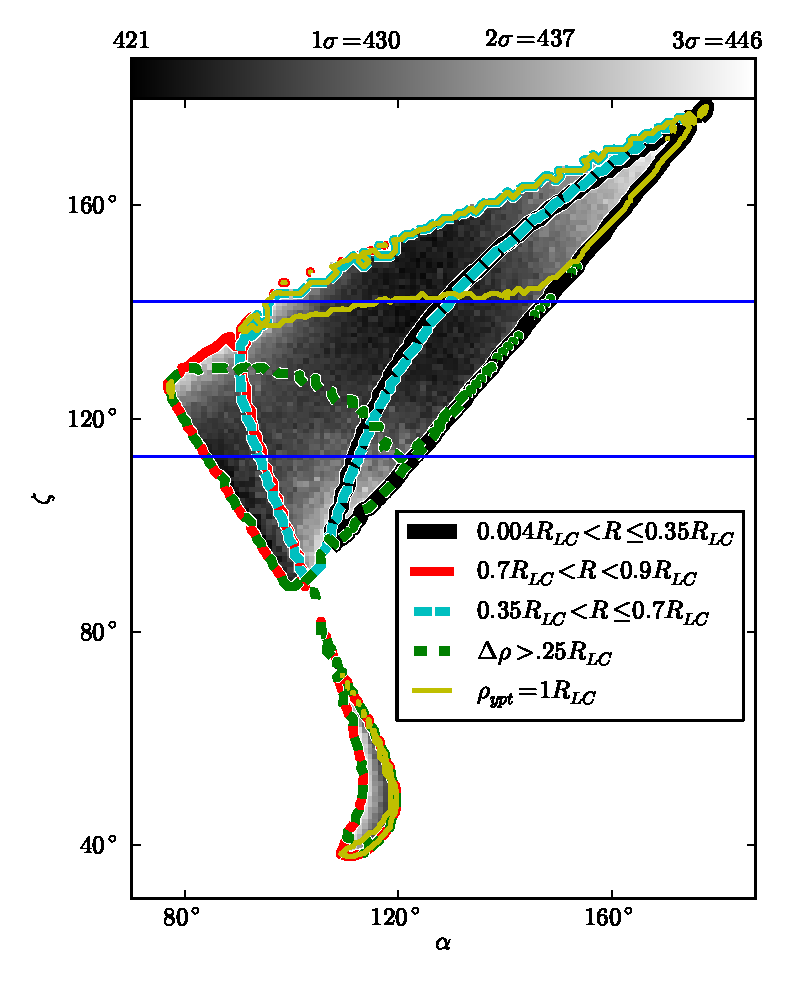
\includegraphics[scale=.8]{chapters/applicationOfNumericalModel/figures/J1420T1.3msMapTot.eps}
\caption[Map of the joint (unreduced) $\chi^{2}$ for polarization data in 10 cm and 20 cm of PSR J1420$-$6048 in the $\alpha$--$\zeta$ plane]{\label{fig:T1.3map}
Map of the joint (unreduced) $\chi^{2}$ for polarization data in 10 cm and 20 cm of PSR J1420$-$6048 in the $\alpha$--$\zeta$ plane. 
The model has a scattering constant of $\tau=1.3$ ms.
Contours of $3\sigma$ are for three ranges of $R$ to show the correlation between $\alpha$, $\zeta$, and altitude and for
$\Delta\rho\leq 0.25R_{\rm{LC}}$ (the most physically inaccurate models) and $\rho_{\rm{ypt}}=1R_{\rm{LC}}$
(the most physically accurate models).  Horizontal blue lines indicate the region favored by X-ray
torus fitting (Section \ref{sec:xray}).
}
\end{center}
\end{figure}


The millisecond pulsar ($P=68$ ms) PSR J1420$-$6048 has 
been studied previously (\citealt{roberts2001multiwavelength};
\citealt{weltevrede2010gamma}).  
The RVM fit in these papers estimated $\alpha>145^\circ$ and $\zeta-\alpha\sim 0\degr5$
(the angle convention used in these papers is different from that used
in this paper and they must be converted.  
See \citealt{everett2001emission} for an explanation and the conversion formula).
This fit is consistent with our results of fitting with the RVM.
Since the effects of interstellar scattering scales 
to the $-4$ power in frequency \citep{lang1971pulse}, 
comparing 10 cm data to 20 cm data reveals that 
the polarization and intensity profile of PSR J1420$-$6048 have 
signs of scattering (Figure~\ref{fig:PlotJ1420intPA}).  
In particular, note the widening of the intensity profile and the flattening
of the polarization sweep at the trailing edge of the intensity components for 
the 20 cm data compared to the 10 cm data.  The scattering
time constant calculated using the \citet{cordes2002ne2001} 
model is $\tau=6.5\e{-2}$ ms.  The ratio of $\tau$
to period (and also the value of dispersion measure or DM) is far larger than that for any of the other
pulsars considered in this paper yet this value is still smaller than 
what would cause the scattering seen by comparing the 10 cm and 20 cm data.
Because of this discrepancy, $\tau$ is a fit parameter in analyzing 
polarization data of PSR J1420$-$6048. 

When fitting the 10 cm data ($\tau\sim0$), the best fit non-scattered model 
is $\alpha=100^{+34(+79)\circ}_{-63(-97)}$, $\zeta=39^{+116(+140)\circ}_{-25(-38)}$, and $R=0.64^{+0.26(+0.26)}_{-0.64(-0.64)}R_{\rm{LC}}$
where errors without (with) parentheses are $1\sigma$ ($3\sigma$) errors.
The error bars on these values are large due to 
the low signal-to-noise in the polarization position
angles and the exact parameter values at 
$\chi^2_{\rm{min}}$ are less valuable than the full range defined by these
error bars.  When fitting the 20 cm polarization data, 
with a small scattering time ($\tau=0.1$ ms), 
the best fit non-scattered model is $\alpha=175^{+2(+3)\circ}_{-6(-18)}$, $\zeta=177^{+1(+1)\circ}_{-4(-14)}$, and 
$R=.37^{+0.10(+0.50)}_{-0.33(-0.37)}R_{\rm{LC}}$ which is drastically different
than the results for the 10 cm data.  In fact the $3\sigma$ multi-dimensional contours as
measured from the individual $\chi^2_{\rm{min}}$ do not overlap.

Physically, we expect that two different 
frequencies should come from different altitudes but we
are making the assumption that they are closely spaced and any systematic error from this assumption
is overpowered by the statistic error.
A combined $\chi^{2}$ from the two sets of data 
(10 cm and 20 cm) at low scattering constants results in 
a minimum region similar to the minimum of fitting 20 cm 
alone (see Figure~\ref{fig:diffTau}, cyan contours $\tau=0.1$ ms).
A combined $\chi^{2}$ from the two sets of data at 
an intermediate scattering constant results in
two distinct minimum regions (see Figure~\ref{fig:diffTau}, 
magenta contours $\tau=0.9$ ms).  
A combined $\chi^{2}$ from the two sets of data 
at high scattering constants results in
a single minimum region (see Figure~\ref{fig:diffTau}, 
green contours $\tau=1.5$ ms).
In the combined $\chi^{2}$, we assume that the altitudes are the same.
Fitting the data with different scattering constants gives drastically different results.
The larger the scattering constant, the better the $\chi^{2}_{\rm{min}}$.  
We can place a practical
limit on the scattering because a large scattering constant results in a distorted intensity 
profile which is not seen in the data.  
Therefore, we did not fit with a scattering constant larger
than $\tau=1.5$ ms since scattering constants much 
larger than this distort the intensity profile.
In Figure~\ref{fig:diffTau}, as the scattering constant increases, the two islands of 
best fit $\chi^2$ seen at the lowest scattering constant merge into a single $\chi^2$ surface.
Because of the drastic decrease in $\chi^{2}_{\rm{min}}$ from increasing the scattering
constant and the merging of the $\chi^{2}_{\rm{min}}$, the true scattering constant 
is $\tau\sim 1.1$--$1.5$ ms.  Additionally, we report $\alpha$, $\zeta$, and $R$ in
Table~\ref{tb:fitJ1420} for select values of $\tau$. 

Further, the error bars on the DM are larger than the shift that we 
expect from including scattering when comparing the two different wavelengths.
The DM reported in \citet{weltevrede2010gamma} 
is $360^{+2}_{-2}$ cm$^{-3}$ pc and the correction to the 
DM from our fitting of scattering time constants with 
error bars are reported in Table~\ref{tb:fitJ1420}.
The $\Delta \rm{DM}$ values are all with in the 2 cm$^{-3}$ 
pc error bars of the original DM up to 
$3\sigma$ from $\chi^2_{\rm{min}}$.

As $\tau$ increases, the best fit values of $\alpha$ and $\zeta$ shift and the $3\sigma$ range
for these values increases drastically.  
Also, the $\chi^2_{\rm{min}}$ values decrease statistically 
significantly from $\tau=0.1$ ms to $\tau=1.5$ ms.  
For $\tau=1.5$ ms, $3\sigma=439$ from $\chi^2_{\rm{min}}$.
The $\chi^2_{\rm{min}}$ for $\tau=0.1$ ms is not within 
this $3\sigma$ of the $\tau=1.5$ ms fit.

Figure~\ref{fig:T1.3map} is the (unreduced) $\chi^2$ map for $\tau=1.3$ ms.  The black,
cyan, and red contours are for $3\sigma$ contours at various altitude ranges, 
illustrating that although the allowed range of altitudes is large for this pulsar, knowledge
of $\alpha$ and $\zeta$ could greatly decrease this 
range because of the correlation between $R$ and
$\alpha$--$\zeta$ pairs.  A large number of fits could be additionally excluded if
cuts of $\Delta\rho$ are applied. 
The green dashed contour corresponds to $\Delta\rho<0.25R_{\rm{LC}}$.
If only fits up to $3\sigma$ with $\rho_{\rm{ypt}}=1R_{\rm{LC}}$ are considered, 
only fits within the yellow
contour on Figure~\ref{fig:T1.3map} would be allowed.


\begin{table}[ht]
\footnotesize
\tabcolsep=0.05cm
\caption{Fit Parameters for PSR J1420$-$6048}
\begin{center}
\def\arraystretch{1.5}
\scalebox{1}{
\begin{tabular}{lccccccccc}
\hline
\hline
 &$\tau$&(Unreduced)&&&\\
DOF&(ms) & $\chi^2_{\rm{min}}$ & $\alpha$ ($^\circ$) & $\zeta$ ($^\circ$) & $R$ ($R_{\rm{LC}}$)\\ 
[.3em]\hline
356-5&.1 & $   480 $ & $  175 ^{+3(+4)}_{-15(-77)} $ & $  177 ^{+1(+2)}_{-13(-86)} $  & $ 0.37 ^{+0.10(+0.52)}_{-0.31(-0.37)} $ \\ \hline
356-5&.9 & $   448 $ & $  166 ^{+13(+13)}_{-76(-81)} $ & $  169 ^{+10(+10)}_{-104(-119)} $  & $ 0.26 ^{+0.64(+0.64)}_{-0.26(-0.26)} $ \\ \hline
356-5&1.3 & $   421 $ & $  126 ^{+22(+51)}_{-46(-50)} $ & $  153 ^{+9(+25)}_{-113(-115)} $  & $ 0.52 ^{0.38(+0.38)}_{-0.52(-0.52)} $ \\ \hline
356-5&1.5 & $   415 $ & $  105 ^{+27(+42)}_{-28(-31)} $ & $  140 ^{+14(+22)}_{-102(-106)} $  & $ 0.58 ^{+0.32(+0.32)}_{-0.44(-0.58)} $ \\ \hline

\end{tabular}}
\tablecomments{Errors reported without (with) parentheses are for $1\sigma$ ($3\sigma$) from $\chi^2_{\rm{min}}$. }
\label{tb:fitJ1420}
\end{center}
\end{table}


\vskip 1.0truecm
\subsubsection{X-Ray Torus of PSR J1420$-$6048}
\label{sec:xray}
\begin{figure}[t!!]
\begin{center}
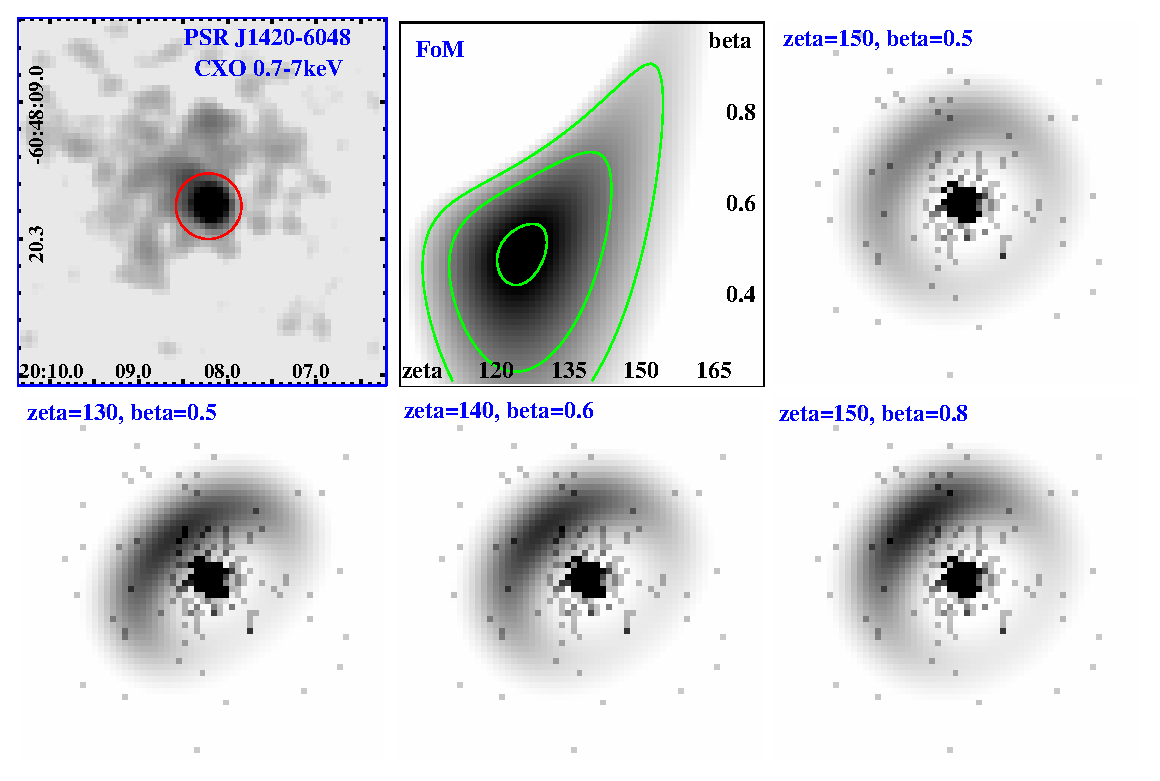
\includegraphics[scale=.8]{chapters/applicationOfNumericalModel/figures/J1420_torfit_comp.eps}
\caption[X-ray pulsar wind nebula of PSR J1420$-$6048]{\label{fig:xraytorus}
X-ray pulsar wind nebula of PSR J1420$-$6048. Upper left shows the pulsar wind nebula structure,
while the figure of merit (FoM) panel show contours of the fit in the $\zeta$--$\beta$ plane. The
other panels show the dependence of the torus shape and brightness on these 
parameters (see Section \ref{sec:xray}).
}
\end{center}
\end{figure}

Young pulsars appear to produce relativistic plasma confined
to the spin equator. When this wind shocks the $e^+/e^-$ pitch angle scatter and
synchrotron radiate, producing an equatorial torus. Since the bulk flow in the
region is mildly relativistic, with expected bulk velocity $\beta \sim 0.3$--$0.7$,
this torus can be Doppler brightened on the side emerging from the plane of the sky.
In several cases, there seems to be a secondary shock along the polar axis producing
polar ``jets'' in the pulsar wind nebula, 
with the jet on the opposite side of the Doppler-enhanced torus
rim, being Doppler boosted. The Crab and Vela pulsars provide classic examples of this
relativistic torus--jet geometry.

\citet{ng2004fitting} and \citet{ng2008fitting} % 2004ApJ...601..479N, 2008ApJ...673..411N
showed how fits to {\it Chandra} X-ray images of such tori can provide useful constraints
on the pulsar spin orientation. For PSR J1420$-$6048, we obtained a 90\,ks {\it Chandra}
ACIS observation (ObSID 12545). We combined this exposure with a 10\,ks archival observation
(ObsID 2794), removing the spacecraft dither and reprocessing the data giving
sub-pixel (EDSER) event positioning, to obtain the best possible image of the compact
PWN surrounding this energetic pulsar.  Figure~\ref{fig:xraytorus} (upper left) shows a lightly smoothed
0.7--7 keV {\it Chandara} image of the combined 
exposure, with a logarithmic stretch. The pulsar point
source is in the red circle. Unfortunately, this pulsar does not show a striking torus
structure, so unlike several other young pulsars, we cannot obtain a high-quality,
model-independent measurement of its spin geometry. Still, the diffuse counts do show
a semi-circular arc of flux, trailing off to the NE. {\it If} we interpret this as an
equatorial torus, we can apply the methods of \citet{ng2008fitting} to constrain the spin
orientation. A few parameters are well measured: the position angle of the symmetry axis
($\Psi = 40^\circ \pm 3^\circ$, measured N through E) and the radius of the ``torus''
($7^{\prime\prime}\pm 1 \farcs 5$) are reasonably 
constrained. In unsmoothed images there is
some evidence for a polar component on a 
$1^{\prime\prime}$--$2^{\prime\prime}$ scale, but this is not well
measured. The parameter of greatest interest to the present study is the inclination
$\zeta$ of the pulsar spin to the Earth line-of-sight.
To minimize sensitivity to point source flux and possible jet structure we fit outside
of the $5^{\prime\prime}$ radius red circle dominated by the central point source.
The main constraint comes from the shape and brightness ratio between the front and
back sides of the torus. The second panel of 
Figure~\ref{fig:xraytorus} shows that this introduces
substantial co-variance between $\zeta$ and the bulk $\beta$ of the post-shock flow.
The best fits are near typical $\beta \sim 0.5$, with $\zeta \approx 125^\circ$.
This is in considerable tension with the larger  $\zeta$ preferred by the polarization position angle
fits to models with small scattering times; 
we only reach  $\zeta \approx 155^\circ$ with a rather aphysical $\beta \sim 0.9$.
This co-variance is visible along the bottom row of torus (+point spread function+jet) models, which show that
as $\zeta$ increases from $130^\circ$ to $150^\circ$, the post-shock Lorentz factor
must grow to maintain a reasonable intensity ratio between the ``front'' and ``back''
sides of the torus. The last panel on the top row shows how with $\zeta=150^\circ$,
$\beta=0.5$, the torus is too face-on and uniform for a good fit to the data.
Thus the X-ray pulsar wind nebula structure agrees with the $\gamma$-ray pulse shape, where the observed
peak separation $\Delta = 0.31$ implies $\zeta \approx 110^\circ$--$140^\circ$, with the largest
$\zeta$ only available in the two-pole caustic picture \citep{romani2010constraining}, which tends to produce
too much unpulsed emission.

Polarization position angle fits with scattering constant $\tau=1.3$ ms as 
discussed in Section \ref{sec:J1420} favor $\zeta$ between $120^\circ$ and $150^\circ$
as can be seen from the color map of Figure~\ref{fig:T1.3map}.  
The measurement of $\zeta$ from the 
X-ray torus fit indicates $\zeta$ between $113^\circ$ 
and $142^\circ$ (from the contours of $2\sigma$).  
The horizontal blue lines on Figure~\ref{fig:T1.3map} 
mark the region of $2\sigma$ set by the X-ray 
torus fitting.  By assuming a
scattering constant, we not only reconcile the fits of 10 cm and 20 cm data but also 
find consistency between radio polarization position angle fits and X-ray torus fits. 

\subsection{PSR J2124$-$3358: A Complex Example}
\label{sec:J2124}

\begin{table*}[t]
\tabcolsep=0.1cm
\caption{Fit Parameters for PSR J2124$-$3358}
\begin{center}
\def\arraystretch{1.5}
\scalebox{0.8}{
\begin{tabular}{lccccccc}
\hline
\hline
& DOF&(Unreduced) $\chi^2_{\rm{min}}$ & $\alpha$ ($^\circ$) & $\zeta$ ($^\circ$) & $R_1$ ($R_{\rm{LC}}$)& $R_2$ ($R_{\rm{LC}}$)& $R_3$ ($R_{\rm{LC}}$)\\ 
[.3em]\hline 

RVM& 536-4&$  2331 $ & $    2 ^{+3(+7)}_{-0(-0)} $ & $    5 ^{+8(+19)}_{-0(-0)} $  &\ldots &\ldots &\ldots \\ \hline

3 Alt & 536-7&$   773 $ & $    2 ^{+7(+12)}_{-1(-1)} $ & $    2 ^{+7(+12)}_{-1(-1)} $ 
& $ 0.05 ^{+0.01(+0.03)}_{-0.00(-0.00)} $ & $ 0.40 ^{+0.01(+0.02)}_{-0.01(-0.03)} $ & $ 0.55 ^{+0.02(+0.04)}_{-0.01(-0.03)} $  \\ \hline


\end{tabular} }
\tablecomments{Errors reported without (with) parentheses are for $1\sigma$ ($3\sigma$) from $\chi^2_{\rm{min}}$.}
\label{tb:fitJ2124} 
\end{center} 
\end{table*}




\begin{figure}[htbp]
\begin{center}
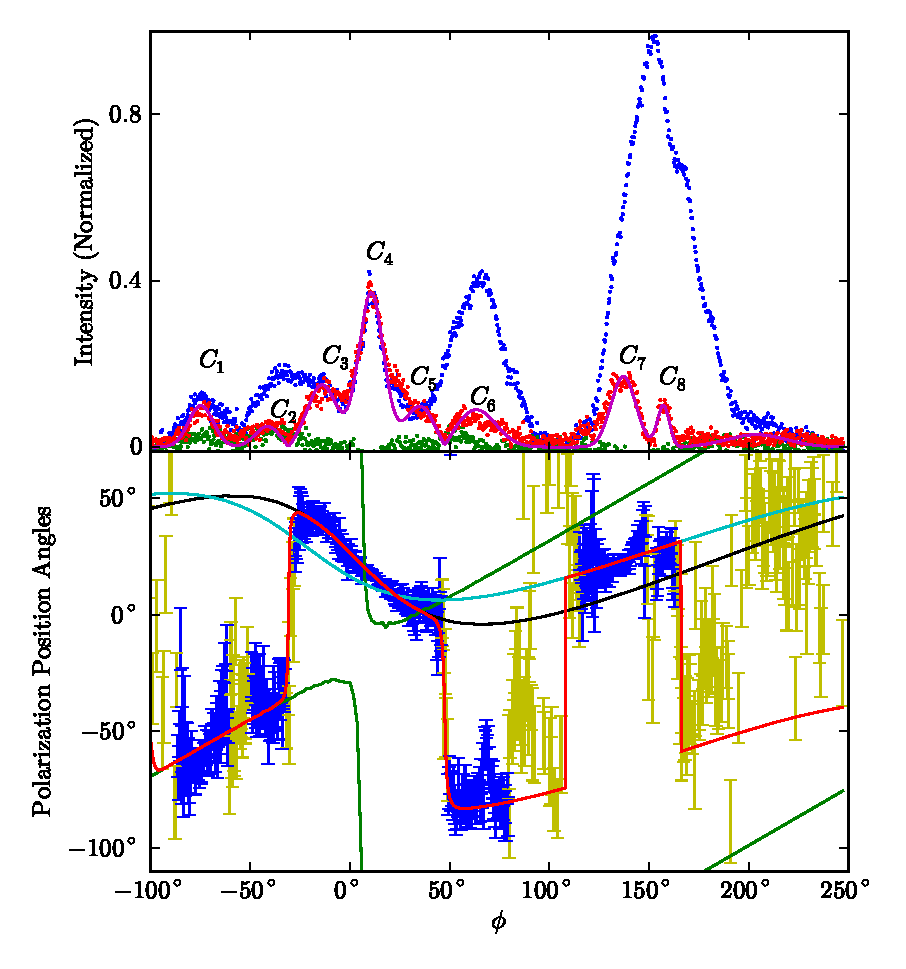
\includegraphics[scale=.8]{chapters/applicationOfNumericalModel/figures/intAndPAJ2124alpha2zeta2.eps}
\caption[Intensity and polarization data for PSR J2124$-$3358 overlaid with model]{\label{fig:PlotJ2124intPA}
In the upper panel, blue points are total radio intensity data for 1.369 GHz, red points are linear polarization intensity data,
and green points are circular polarization intensity data for PSR J2124$-$3358.  The solid magenta line in the upper panel is
the model linear intensity used in fitting.  In the bottom panel, blue error bars are polarization position angles
used in the fit and yellow error bars are polarization position angles excluded by error bar cuts.
The model polarization comes from
a fit with (unreduced) $\chi^2=773$ and parameters $\alpha=2^{\circ}$ and $\zeta=2^{\circ}$.  The green solid line is the polarization for
a model with $R_{1}=0.05R_{\rm{LC}}$ (associated with intensity components $C_1$ and $C_2$),
the black solid line is the polarization for a model with $R_{2}=0.40R_{\rm{LC}}$ (associated with intensity components $C_3$, $C_4$, and $C_5$),
and the cyan solid line is the polarization for a model with $R_{2}=0.55R_{\rm{LC}}$
(associated with intensity components $C_6$, $C_7$, and $C_8$).  
We assumed that the polarization associated with
components $C_1$, $C_2$, and $C_6$ are orthogonal to the polarization associated with
components $C_3$, $C_4$, $C_5$, $C_7$, and $C_8$.
The red solid line is the model
polarization of the three altitudes weighted by the model intensity.  There are clearly 
features in the data that are not captured by the model but the overall structure of 
the polarization is captured.
A phase of zero is the point
of closest encounter to the magnetic axis in the model.
}
\end{center}
\end{figure}


\begin{figure}[t!!]
\begin{center}
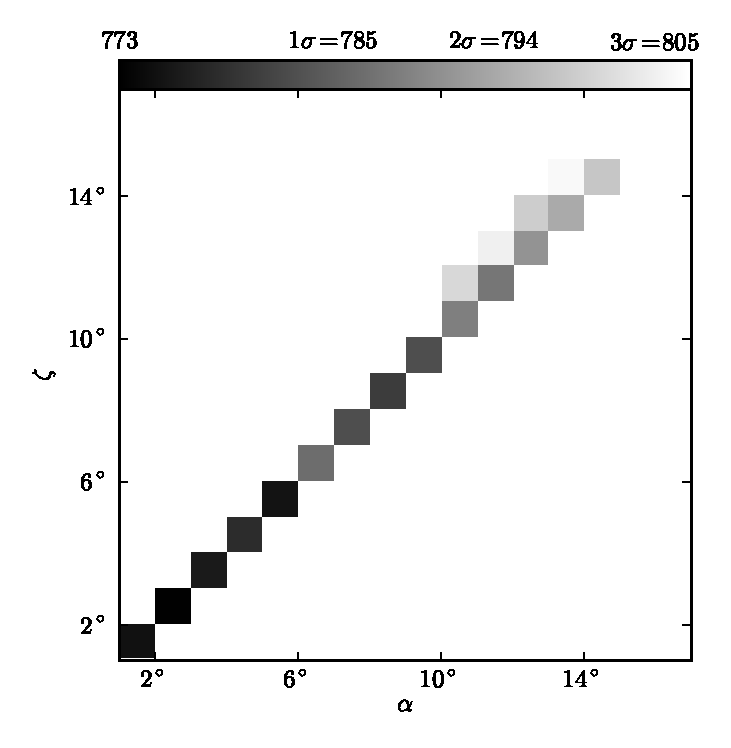
\includegraphics[scale=.8]{chapters/applicationOfNumericalModel/figures/J2124-3358Map.eps}
\caption[Map of (unreduced) $\chi^{2}$ for PSR J2124$-$3358 in the $\alpha$--$\zeta$ plane]{\label{fig:MapJ2124}
Map of (unreduced) $\chi^{2}$ for PSR J2124$-$3358 in the $\alpha$--$\zeta$ plane.
All of the fitted models within $3\sigma$ from $\chi^2_{\rm{min}}$ have a phase of emission
that is within the phase of emission predicted by the models and thus $\rho_{\rm{ypt}}=1R_{\rm{LC}}$
is acceptable.
}
\end{center}
\end{figure}


PSR J2124$-$3358 is yet another millisecond pulsar ($P=4.931$ ms).  
Plotted in Figure~\ref{fig:PlotJ2124intPA}
is the polarization and intensity profile for this pulsar at 1.369 GHz.  
The pulsar PSR J2124$-$3358 has emission at practically 
all phases of the period.  The polarization position angles
are complicated but can be greatly simplified by assuming orthogonal mode jumps
at the appropriate components.  We assumed that the polarization associated with
components $C_1$, $C_2$, and $C_6$ are orthogonal to the polarization associated with
components $C_3$, $C_4$, $C_5$, $C_7$,  
and $C_8$ as labeled in Figure~\ref{fig:PlotJ2124intPA}.
With these orthogonal mode jumps, the polarization forms a close-to-continuous 
sweep and the RVM can be reasonably fit to the data.  Table~\ref{tb:fitJ2124} 
reports the best fit values and (unreduced) $\chi^2_{\rm{min}}$ for this fit.  

With the assumption of multiple altitudes and mode jumps, the polarization was also fit.
More than three altitudes did not significantly improve the fit.  
Also plotted in Figure~\ref{fig:PlotJ2124intPA} (top panel) 
is the best fit polarization model with multiple 
altitudes.  The polarization associated with components $C_1$ and $C_2$ is assigned one 
altitude ($R_1$); the polarization associated with components $C_3$, $C_4$, and $C_5$ is assigned the second
altitude ($R_2$); and the polarization associated with components 
$C_6$, $C_7$, and $C_8$ is assigned the third altitude ($R_3$).
The fit is far from perfect and does not capture the many bumps 
and wiggles in the polarization data.  The model does capture the overall
curvature of the polarization and significantly decreases the $\chi^2$ (Table~\ref{tb:fitJ2124})
although the $\alpha$ and $\zeta$ values do not change drastically between the two fits.
For the RVM (unreduced) $\chi^2_{\rm{min}}=2331$ and 
for the three-altitude model (unreduced) $\chi^2_{\rm{min}}=773$.
The $F$-test between RVM and the two-altitude model gives $F=355.4$, 
$\rm{DOF}_1=3$, and $\rm{DOF}_2=529$. The probability of
exceeding this $F$ is $\rm{Prob}\sim 0$, indicating the addition of altitude to the model
is highly statistically significant.

The curvature direction of the bridging polarization sweep between orthogonal
mode jumps is important here similar to the 
polarization of PSR J0023$+$0923 in Section~\ref{sec:J0023}.
As discussed in Section~\ref{sec:MAISOM}, for a single-altitude polarization sweep
with an orthogonal mode jump, the bridging section of 
polarization between the two modes will have
the opposite curvature of that of the 
original sweep due to forward scattering.  In PSR J2124$-$3358
between the polarization components associated with the intensity components $C_5$ and $C_6$, 
the bridging sweep direction has a negative curvature and the original sweep direction
is also negative.  This indicates that the polarization of these two components are not exactly
$90^\circ$, which is consistent with a 
multi-altitude model that has non-$90^\circ$ orthogonal jumps
between altitudes.

The values for $R_1$, $R_2$, and $R_3$ are quite restrictive and the statistical error
bars on these values are quite small.  These values are small because very
few altitude combinations capture the subtle difference between polarization
associated with the various components; for instance, note the rather large
offset between the black and cyan solid lines in Figure~\ref{fig:PlotJ2124intPA}
which represent model polarization from $R_{1}$ and $R_{2}$.  Only very 
particular sets of altitude will result in polarization with this amount
of vertical shift.
Also, $\rho_{\rm{ypt}}=1 R_{\rm{LC}}$ for all fits within
the $3\sigma$ bound of $\chi^2_{\rm{min}}$ due to the small geometrical angles 
($\alpha$ and $\zeta$, see Figure~\ref{fig:MapJ2124}).


\section{Conclusion}
\label{sec:conclusion}
In this paper, we attempted to push the limit of what we can 
learn from geometrical-based models applied to radio polarization.
We have shown that this model can explain polarization for 
which the RVM fails (partially or fully) and can significantly alter 
fit parameters ($\alpha$ and $\zeta$) obtained from the RVM.
We have shown that a handful of physical 
effects can alter our understanding of the geometry 
of millisecond and young pulsar radio emission.  
Additionally, we provided statistical comparisons to simpler 
models to quantify the significance of adding 
these physical phenomena to the model.

Both PSR J0023$+$0923 and PSR J1024$-$0719 clearly illustrate
how multi-altitudes can capture the non-$90^\circ$ jumps seen in the
position angle sweeps of the millisecond pulsar population.
PSR J1057$-$5226 and PSR J1744$-$1134 illustrate the need 
for finite altitude and $\rho_{\rm{ypt}}<R_{\rm{LC}}$
to fully explain the large phase range of the emission seen in the data.
PSR J1420$-$6048 illustrates how scattering affects can rectify
discrepancies seen between multi-wavelength data.
Finally, PSR J2124$-$3358 is a typical worst-case radio polarization from a millisecond pulsar.
Despite its clear non-RVM characteristics, we were
able to capture the overall structure of the polarization position angles sweep
with finite and multiple altitudes and orthogonal mode jumps.

The RVM is not accurate for the radio
polarization sweeps of these energetic pulsars.  First, this emission
originated from a significant fraction of the light cylinder which necessitates
numerical calculation of this radio polarization.  Additionally, non-$90^\circ$
jumps cannot be explained by simple orthogonal mode jumps and some polarization 
is scattered by the interstellar medium.
Polarization of millisecond pulsars is notoriously hard to model
and very few studies have attempted to tackle these objects.
That we can explain some of the polarization of these pulsars
is a significant step in the correct direction. 
This is a methods paper; with various example 
polarization data from a number of pulsars, we have shown that this 
method of using physically motivated, geometrically based 
phenomena can explain the inconsistencies of simpler models.  



\acknowledgements
We greatly thank R. N. Manchester for supplying 
radio data for PSR J1024$-$0719, PSR J1744$-$1134, and PSR J2124$-$3358 which is
published in \cite{yan2011polarization}.
We also owe many thanks to S. Johnston (2012, private correspondence) 
for supplying radio data for
PSR J1057$-$5226 and PSR J1420$-$6048 and to J. W. T. Hessels for supplying
radio data for PSR J0023$+$0923 (J. W. T. Hessels et al. in preparation).
Roger W. Romani prepared figures and wrote the section on X-ray analysis of PSR J1420$-$6048.
Support for this project was provided in part by grants GO1-12073X and
G03-14057A from the Smithsonian Astrophysical Observatory. This work
was also supported in part by NASA grants NNX10AP65G and NAS5-00147.
This work has been supproted by the Stanford Office of the Vice Provost
of Graduate Education DARE Doctoral Fellowship Program to H.A.C.


\chapter[Characterization]{Characterization of Pulsars and Sub-Luminous Populations}
\label{chapter:collaborationWork}

This chapter focuses on work done in collaborations with others.
Main contributions are in modeling polarization position angle data
using the rotating vector model (RVM) and the numerical model. 
Example work will include use
of the models 
for general characterization of pulsars
and for a population study of $\gamma$-ray sub-luminous pulsars.
Because of the collaborative nature of the
work, this chapter will also focus on the broader use of polarization
data in conjunction with other types of data.
For the most part, $\gamma$-ray
modeling was performed by Roger W. Romani.

First, We will discuss the paper ``PSRs J$0248+6021$ and J$2240+5832$: Young Pulsars 
in the Northern Galactic Plane. Discovery, Timing, and Gamma-ray observations''
\citep{theureau2011psrs} in which two pulsars are reported as detected in the $\gamma$-ray
by the {\it Fermi} Large Area Telescope.  Many properties of the pulsars are characterized
using $\gamma$-ray and radio data.

PSR J1119-6127 is likewise characterized in ``Observations of Energetic High Magnetic Field Pulsars with the
{\it Fermi} Large Area Telescope'' \citep{parent2011observations}.  
A number of high magnetic field pulsars are discussed in the paper and PSR J1119-6127
is analyzed with a single-altitude polarization model.

In ``Broad-Band KeV to MeV Characteristics Of Soft Gamma-Ray Pulsar PSR J1513$-$5908''
\citep{hartogJ1513}, the pulsar PSR J1513$-$5908 (B1509$-$58) is analyzed in a 
number of wavelengths using revisited and updated data.  We analyze the
radio polarization using a single-altitude model.

The pulsar PSR J0737$-$3039A is analyzed using a two-altitude 
polarization model in ``{\it Fermi} LAT Pulsed
Detection of PSR J0737$-$3039A in the Double Pulsar System''.
We also include scattering effects in this model although it 
is difficult to reproduce the scattering effects seen in the data.  
This pulsar has complex polarization, which we selectively
cut.  This pulsar is particularly interesting because few
mildly spun-up pulsars have been detected in the $\gamma$-rays.

Finally, We will discuss the paper ``Sub-luminous $\gamma$-Ray Pulsars''
\citep{romani2011sub}.  The paper examines a number of young radio pulsars
that are weak in the $\gamma$-rays.  We try to determine
whether this sub-luminosity is due to
aligned geometry
using geometric constraints 
(including six pulsars for which we perform analysis using radio polarization).


\section{PSR J0248$+$6021 and PSR J2240$+$5832: Characterizing Young Pulsars with RVM}
\paperref{This section is based on work done for
``PSRs J0248$+$6021 and J2240$+$5832: Young Pulsars in the Northern Galactic
Plane. Discovery, Timing, and $\gamma$-Ray Observations''
\citep{theureau2011psrs}. }


\begin{figure}[t!!]
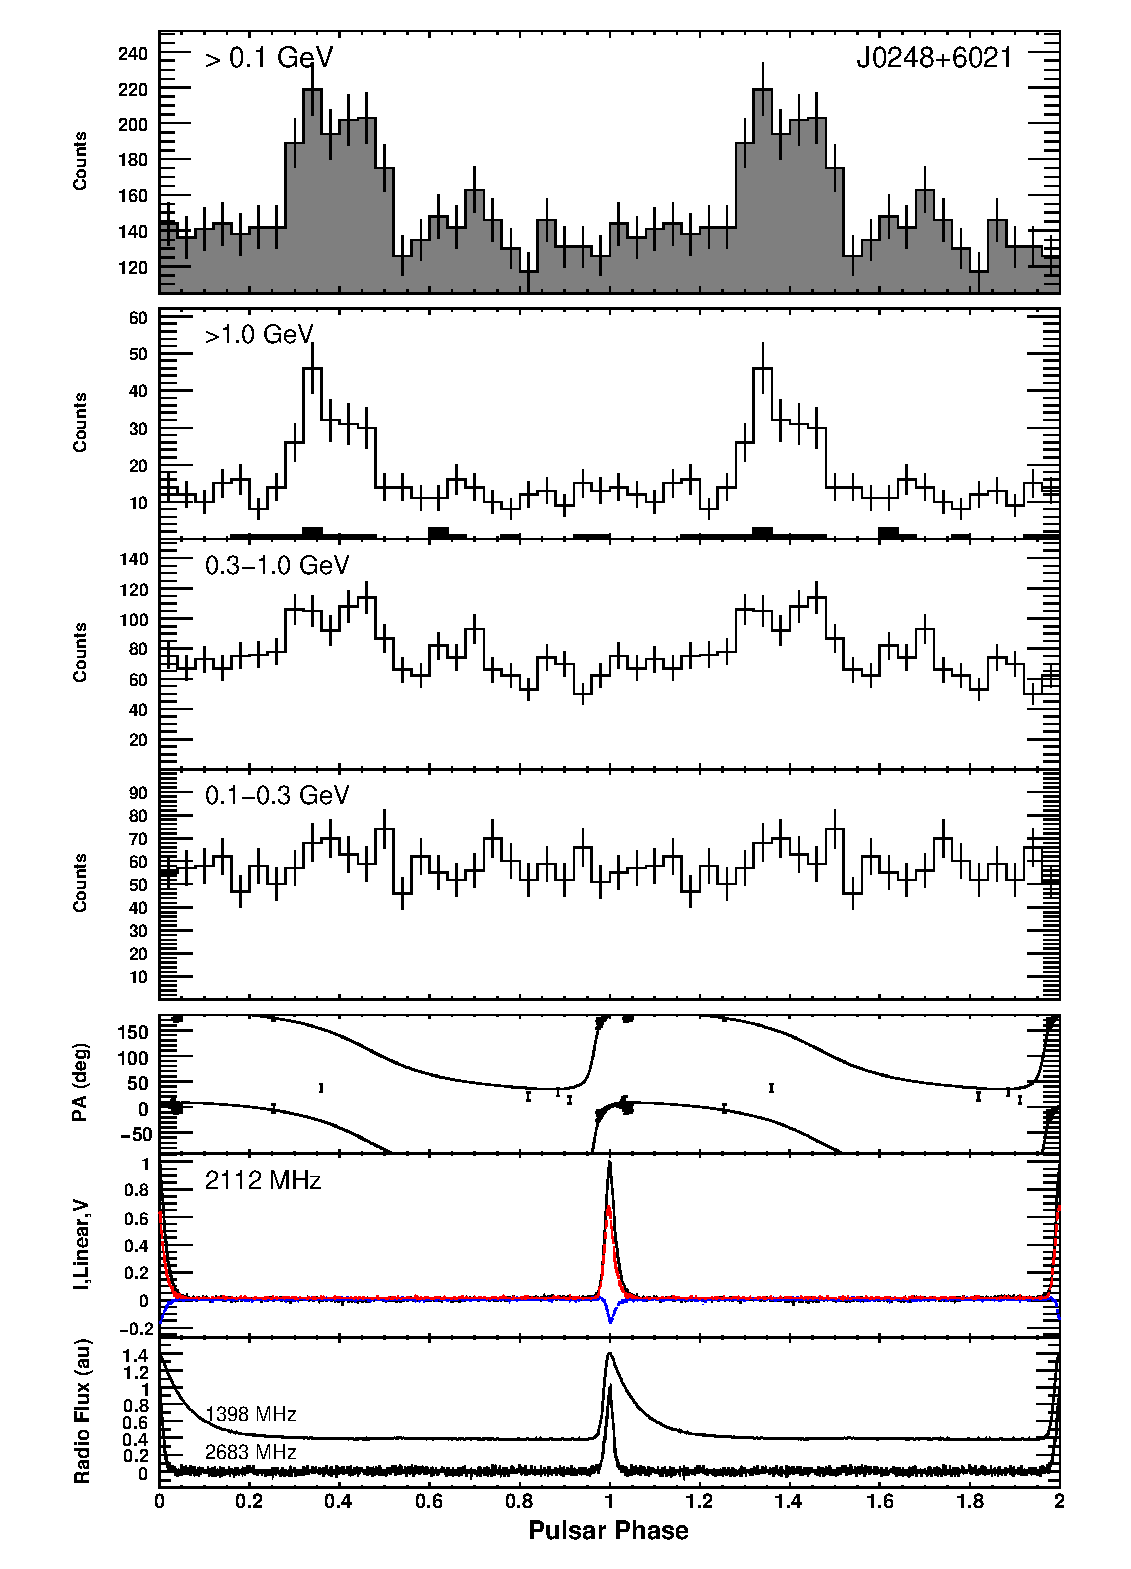
\includegraphics[width=0.5\textwidth]{chapters/multiWaveLength/figures/J0248+6021_catalog_lightcurve.eps}
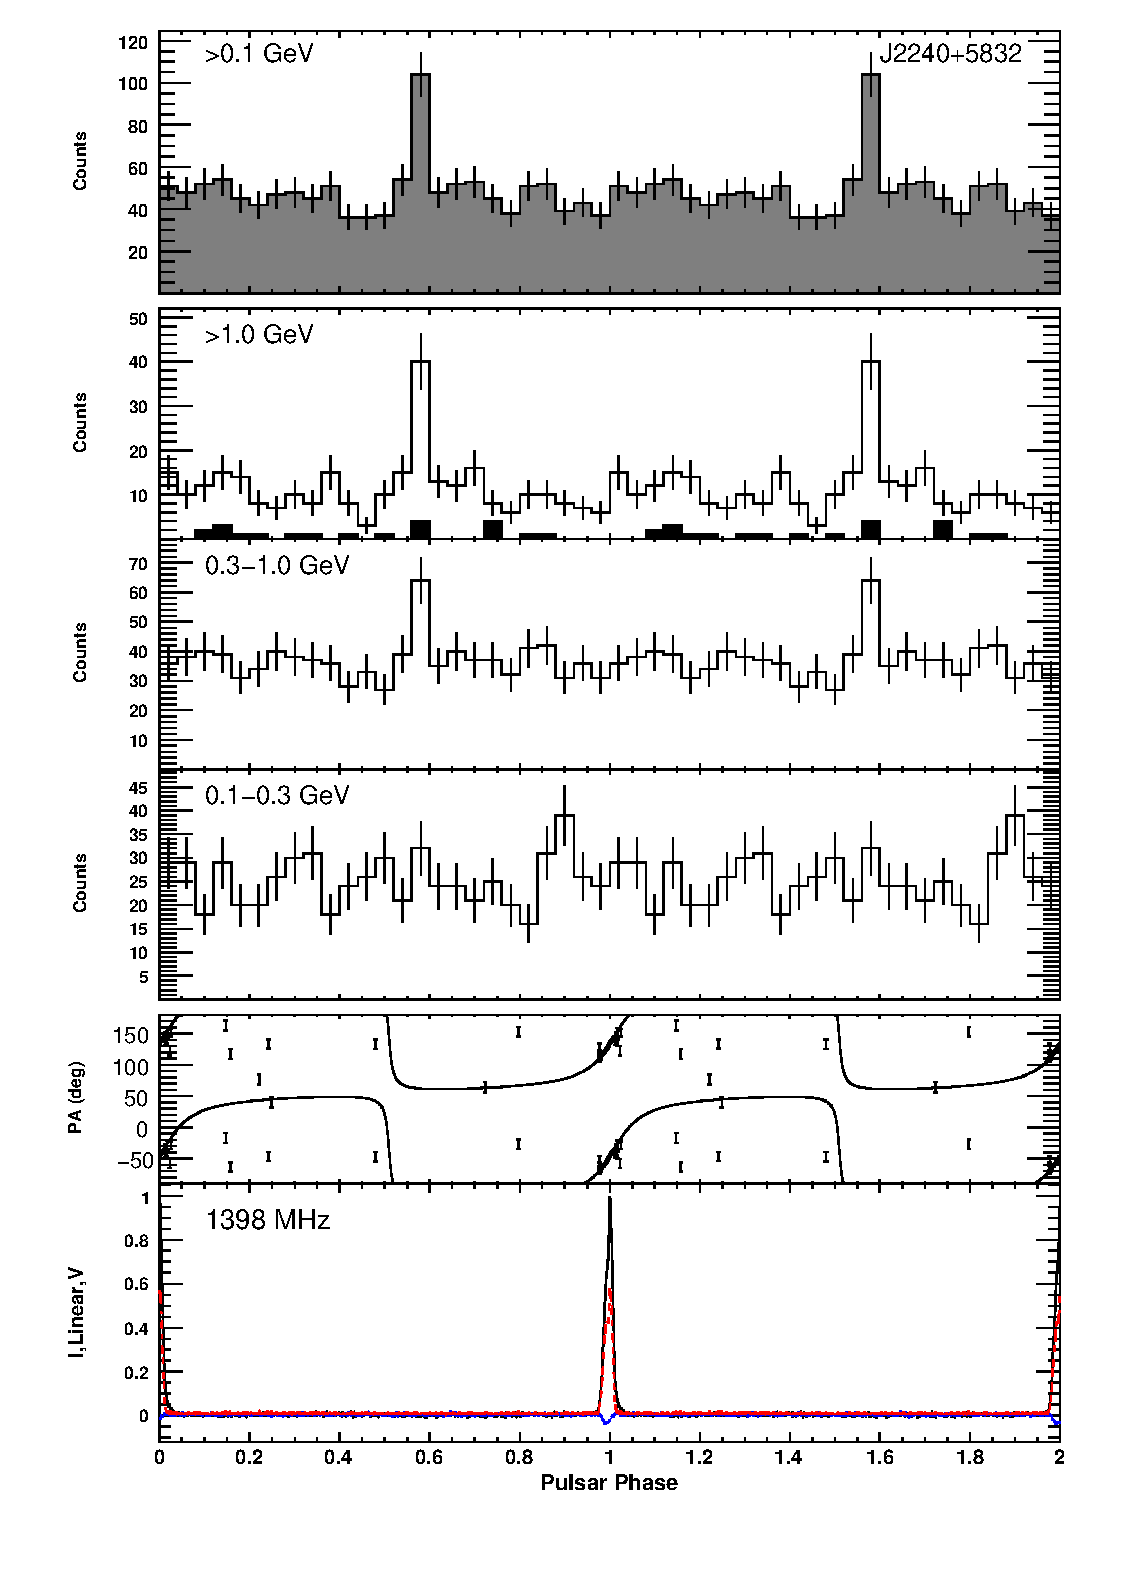
\includegraphics[width=0.5\textwidth]{chapters/multiWaveLength/figures/J2240+5832_catalog_lightcurve.eps}
\caption[Phase-aligned $\gamma$-ray and radio light curves for PSR J0248$+$6021 and PSR J2240$+$5832 obtained with
the \emph{Fermi} Large Area Telescope and the Nan\c cay Radio Telescope]{
Figure taken from \cite{theureau2011psrs}.
Phase-aligned $\gamma$-ray and radio light curves for PSR J0248$+$6021 and PSR J2240$+$5832 obtained with 
the \emph{Fermi} Large Area Telescope and the Nan\c cay Radio Telescope. 
The bottom panel for PSR J0248$+$6021 show the radio profiles at three frequencies. 
The second panel from the bottom
for PSR J0248$+$6021 and the bottom panel for PSR J2240$+$5832 
show the degree of linear (red dashed) and circular
polarizations (blue dotted), as well as the linear polarization position angle and a RVM fit.
The other panels show the
$\gamma$-ray light curve data in different energy bands. Two rotations are shown for clarity.}
\label{phasos}
\end{figure}

\begin{figure}[t!!]
\begin{center}
\includegraphics[width=0.8\textwidth]{chapters/multiWaveLength/figures/J0244Alpha46Zeta52Offset2.53133ANDJ2238Alpha108Zeta123Offsetneg45.818.ps}
\caption[Expanded view of the radio polarization position angle sweep near the peak in radio intensity]{Figure taken from \cite{theureau2011psrs}.
Expanded view of the radio polarization position angle sweep near the peak in radio intensity. 
The red points show the data used in the RVM fit. The black points failed the selection cuts
described in the text. Top two frames are data for PSR J2240$+$5832 at 1.4 GHz. The RVM curve shown corresponds to $\alpha = 108^\circ$ and $\zeta = 123^\circ$. Bottom two frames are data for PSR J0248+6021
at 2.1 GHz. The RVM curve shown corresponds to $\alpha = 46^\circ$ and $\zeta =52^\circ$.  \label{PolarZoom}
}
\end{center}
\end{figure}

\begin{figure}[t!!]
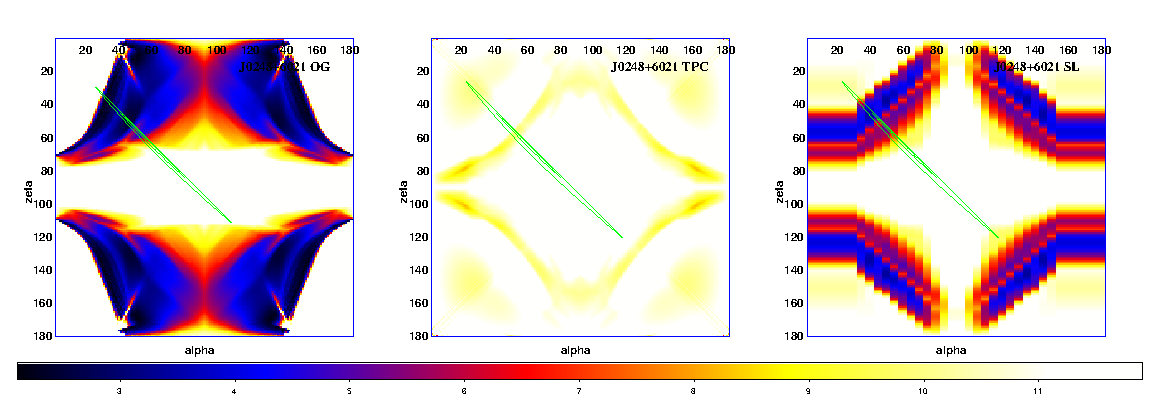
\includegraphics[width=1\textwidth]{chapters/multiWaveLength/figures/New_J0248_OGTPCSL.eps}
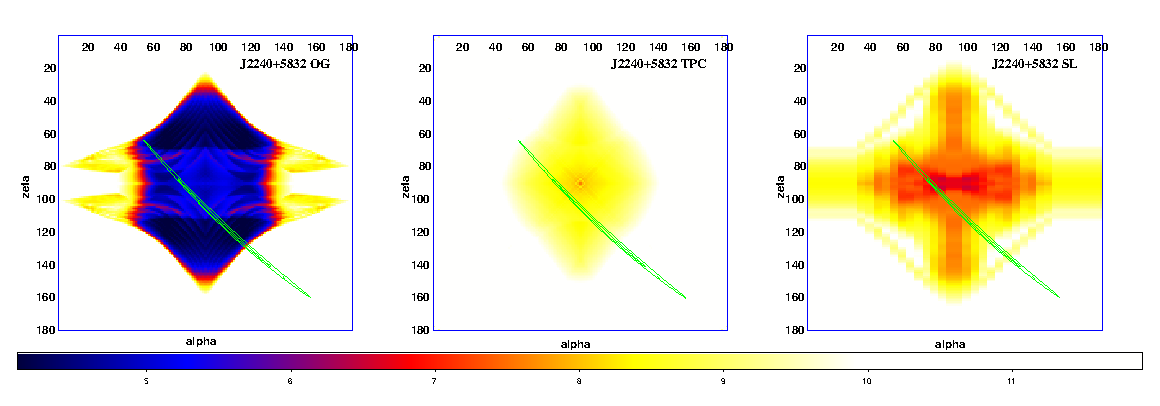
\includegraphics[width=1\textwidth]{chapters/multiWaveLength/figures/New_J2240_OGTPCSL.eps}
\caption[Pulsar geometry and emission modeling fit map for PSR J0248$+$6021 and PSR J2240$+$5832 in the $\alpha$--$\zeta$ plane]{Figure taken from \cite{theureau2011psrs}.
Pulsar geometry and emission modeling fit map for PSR J0248$+$6021 and PSR J2240$+$5832
in the $\alpha$--$\zeta$ plane. Green 
contours show the RVM fit to the radio polarization data. 
Contours are at $\delta(\chi^2/\text{Degree of Freedom}) = 0.25$ and $0.5$ above the minimum $\chi^2/\text{Degree of Freedom}$ of 1.6
for PSR J0248$+$6021 and $\delta(\chi^2/\text{Degree of Freedom}) = 0.4$ and $0.8$ above the minimum $\chi^2/\text{Degree of Freedom}$ of 5.1
for PSR J2240$+$5832.
The color backgrounds are $\chi_3$ maps of the fit to the observed $>100$\,MeV
pulse profile for the outer gap model (left),
the two-pole caustic model (middle), and the separatrix layer model (right), 
at different values of the magnetic inclination,
$\alpha$, and the minimum angle to the line-of-sight, $\zeta$ \citep{romani2010constraining}.
Each panel has the same color scale, where dark colors represent better fits. The
preferred models lie along the green RVM-selected band.
}
\label{OGTPC}
\end{figure}


PSR J0248$+$6021 ($P=217$ ms) and PSR J2240$+$5832 ($P=140$ms) are young pulsars first discovered in the radio
\citep{foster1997fast,ray1999j0248+}.  The polarization sweep for both pulsars is relatively smooth
such that likely only a single-altitude component contributes to the emission.

For these two pulsars, we applied both the RVM and $\gamma$-ray light curve models
to the available data.
Figure~\ref{phasos} shows the light curves at various wavelengths
as well as the polarization data.
Modeling results indicate that the $\gamma$-ray emission from PSR J0248$+$6021
is from a merged double $\gamma$-ray peak while the emission from 
PSR J2240$+$5832 is from a narrow caustic.
The paper discusses various measurements of the
pulsars PSR J0248$+$6021 and PSR J2240$+$5832 such as
flux density, proper motion, dispersion measure, kick velocity, and rotation
measure. 

We applied the RVM to the polarization data of 
PSR J0248$+$6021 (2.1 GHz) and PSR J2240$+$5832 (1.4 GHz).  
We cut on polarization with error bars greater than
 $\pm 2^\circ$.
The polarization position angle sweeps are flattened
due to scattering.  Data at 1.4 GHz was avaliable for PSR J0248$+$6021
but appeared distorted by scatter so only the 2.1 GHz data was used.
Red error bars on Figure~\ref{PolarZoom} show points
used in the fitting procedure.  

For PSR J0248$+$6021, the best fits give geometric angles $\beta\sim5^\circ$ 
(where $\beta=\zeta-\alpha$) and $\alpha$ between $25^\circ$ and $110^\circ$.
The best $\chi^2$ is 86.6 with reduced $\chi_{\rm{min}}^2=1.6$.
For PSR J2240$+$5832, the best fits give geometric angles $\beta\sim16^\circ$ and $\alpha$ between $75^\circ$ and $130^\circ$
although plausible solutions extended to $\alpha$ between $10^\circ$ and $150^\circ$.
The best $\chi^2$ is 86.6 with reduced $\chi_{\rm{min}}^2=1.6$.
Figure~\ref{PolarZoom} additionally shows reasonable model polarization sweeps
overlaid on data points.

On Figure~\ref{OGTPC}, green contours trace the best fit RVM in the $\alpha$-$\zeta$ plane.
The colored maps show best fit outer gap model, two-pole caustic model, 
and separatrix layer model \citep{bai2010modeling} to the $\gamma$-ray data.
The weighting used is the $\chi_3$ of \cite{romani2010constraining}.
For PSR J0248$+$6021, the best fit overlap between outer gap and RVM
model is $\alpha=46^\circ$ and $\zeta=52^\circ$.
For PSR J2240$+$5832, the best fit overlap between outer gap and RVM
models is $\alpha=101^\circ$ and $\zeta=117^\circ$.
Overall, the outer gap model seemed to be more consistent
with the polarization model results
than the other $\gamma$-ray models.





\section{PSR J1119$-$6127: Characterization a High Magnetic Field Pulsar with Single-Altitude Model}

\paperref{This section is based on work done for
``Observations of Energetic High Magnetic Field Pulsars with the
\it{Fermi} Large Area Telescope'' \citep{parent2011observations}.}

\begin{figure}[t!!]
%\begin{center}
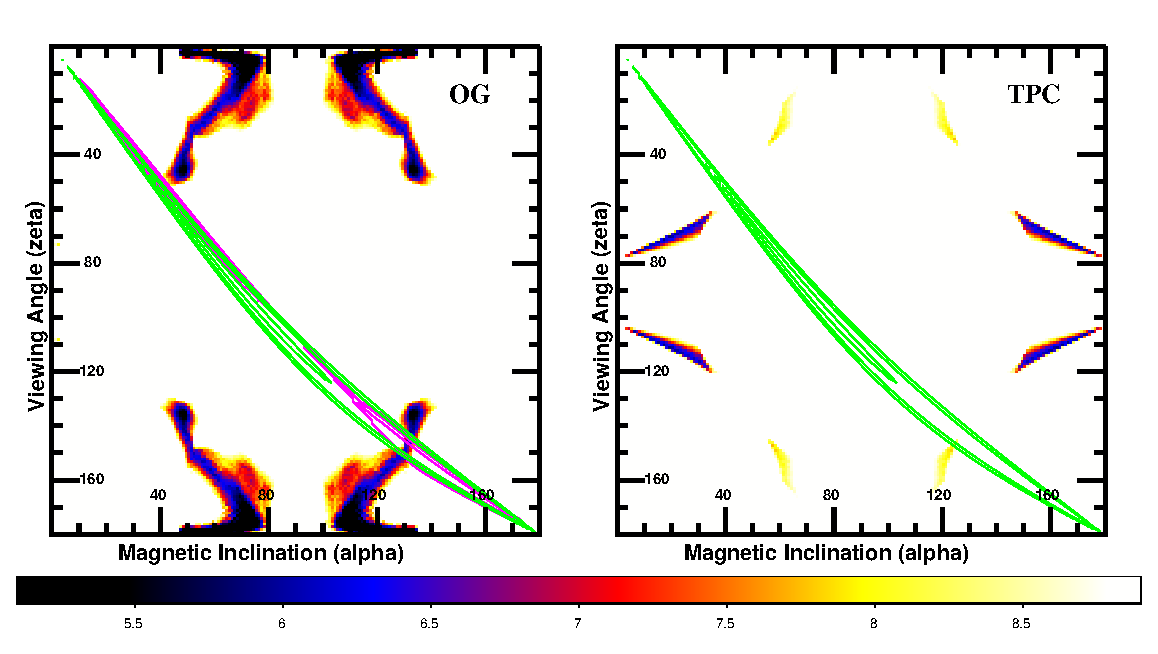
\includegraphics[width=0.99\textwidth]{chapters/multiWaveLength/figures/HBP_fig3_rev.eps}
\caption[Pulsar geometry and emission modeling fit map for PSR~J1119$-$6127 with the outer gap
(left panel) and the two-pole caustic (right panel) models in the $\alpha$--$\zeta$ plane]{
Figure taken from \cite{parent2011observations}.
Pulsar geometry and emission modeling fit map for PSR~J1119$-$6127 with the outer gap
(left panel) and the two-pole caustic (right panel) models in the $\alpha$--$\zeta$ plane. Green contours show
the RVM fit to the \cite{weltevrede2011glitch} radio polarization data. For
the left panel we also show the polarization fit for finite-altitude, open zone
radio emission ($R=0.09\,R_{\rm{LC}}$, magenta contours). Contours are at
1.5, 2.5, and 3.5 times the minimum value of the reduced
$\chi^2 = 0.85$. The background color scale gives the $\chi_3$ statistic fit to
the observed $> 500$\,MeV $\gamma$-ray pulse profile. The color scales in the panels are the
same, with dark colors representing better fits. Preferred models lie along the
diagonal polarization fit band. \label{fig:roger_goodness}}
%\end{center}
\end{figure}

\begin{figure}
\begin{center}
\includegraphics[scale=0.75]{chapters/multiWaveLength/figures/HBP_fig4_rev.eps}
\caption[Light curves and radio polarization of PSR~J1119$-$6127 overlaid with models]{
Figure taken from \cite{parent2011observations}.
Light curves and polarization of PSR~J1119$-$6127 overlaid with models. The bottom panel shows the Parkes
radio light curve in the two peaked (post-glitch) mode, which provides the best
model constraints. The corresponding radio polarization position angle data are
shown (right scale) in the upper panel. The model pulsar phase ($\phi_{\rm{B}}$, bottom axis) is
referenced to the closest approach of the magnetic axis to the Earth
line-of-sight, as fit from the polarization sweep. The sweep rate maximum
(green arrow) and pulse profile offsets (magenta arrow) are shown, with good
matches to the observed radio data for an altitude of $R=0.09 R_{\rm{LC}}$. The
upper panel shows the {\it Fermi} pulse profile (left scale) and model outer gap (solid line)
and two-pole caustic (dashed line) profiles. These are best-fit profiles (geometric angles
in the legend) and the phase is referenced to the radio-determined phase of the
magnetic axis. The $\gamma$-ray background, shown by the dotted line, was
estimated using an annular ring centered on the radio position with inner and
outer radii of 0.5\degr\ and 1.5\degr\ respectively, during the off-pulse
region. \label{fig:roger_lcs} } \end{center}
\end{figure}

In the paper \cite{parent2011observations}, detection 
with the {\it Fermi} Large Area Telescope
of PSR J1119-6127 (Period $=0.408s$) and 
upper limits of pulsars PSR J1718-3718, PSR J1734-3333 and PSR J1846-0258
are reported and criteria for non-detection are discussed.
These pulsars have high magnetic fields.
In the paper, the spectrum of PSR J1119-6127 is concluded to be more 
similar to a young pulsar rather than a magnetar as might
be expected from such a high magnetic field.

Data used to analyze the radio polarization was
taken during a 
glitch recovery in PSR J1119-6127 wherein
more data per phase was available.
Because of the larger number of avaliable data points,
modeling the polarization position
angles was more constraining.
Data analysis details are given in 
\cite{weltevrede2010pulsar} and \cite{hobbs2004long}.

In the $\gamma$-ray modeling, both two-pole caustic
and outer gap models were tested with
$w=0.02$.  Results of these fittings are seen in 
Figure~\ref{fig:roger_goodness}. 
The figure of merit here is the  
$\chi_3$ weighting defined in \cite{romani2010constraining}.
Additionally, on the plot are the  
RVM fit contour results in green as well as a numerical 
single-altitude model fit contour in magenta.  
Two-pole caustic fitting results and the polarization
fitting results have poor overlap compared to the outer gap model.
The best models are at $\alpha=125^\circ$ to $130^\circ$
and $\zeta=140^\circ$ to $150^\circ$ for the outer
gap model and at $\alpha=125^\circ$ and $\zeta=145^\circ$
for the two-pole caustic model. 
The two models give similar geometry angles but 
the outer gap model is a better
fit over a larger parameter space as can be seen in Figure~\ref{fig:roger_lcs}

The best fit parameters for polarization
modeling yield reduced $\chi^2$ of 1.1
The altitude of emission derived
from polarization fitting is $0.1R_{\rm{LC}}$.
It is interesting to note that 
using the BCW model yields lower altitudes 
\citep{weltevrede2011glitch} and requires smaller
$\alpha$ for emission originating in the open zone.




\section{PSR J1513$-$5908: Characterizing a Soft $\gamma$-ray Pulsar with Single-Altitude Model}
\paperref{
This section is based on work done for
``Broad-Band KeV to MeV Characteristics of Soft $\gamma$-Ray Pulsar PSR J1513$-$5908''
\citep{hartogJ1513}.}

\begin{figure}[htbp]
\begin{center}
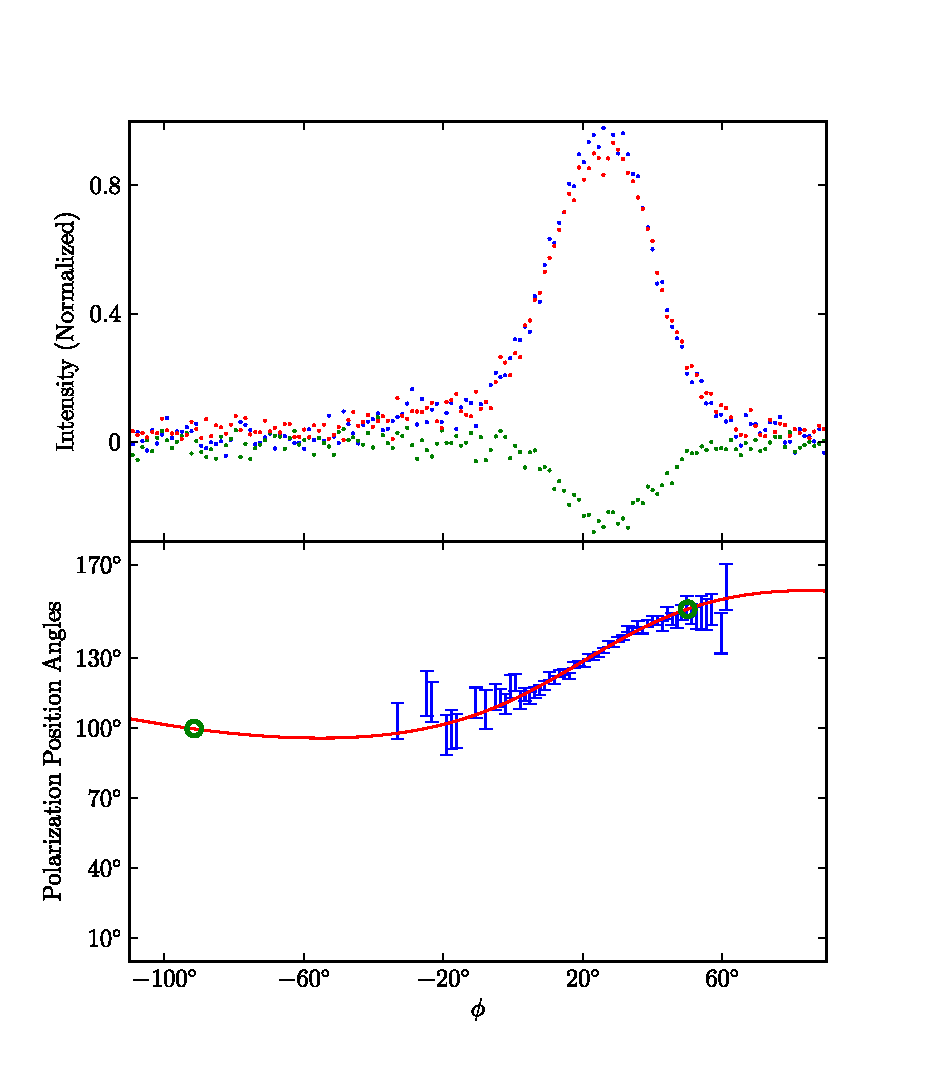
\includegraphics[scale=.8]{chapters/multiWaveLength/figures/intAndPAJ1513alpha153zeta133.eps}
\caption[Intensity and polarization data for PSR J1513$-$5908 overlaid with model]{\label{fig:intAndPAJ1513alpha153zeta133}
Figure taken from \cite{hartogJ1513}.
Intensity and polarization data for PSR J1513$-$5908 overlaid with model.
In the upper panel, blue points are total intensity data, red points are linear polarization intensity data,
and green points are circular polarization intensity data for PSR J1513$-$5908 at 20 cm.
In the bottom panel, blue error bars are polarization position angles
used in the fit. 
The red solid line is the fit model
polarization with $R=0.24R_{\rm{LC}}$, $\alpha=153^{\circ}$, and $\zeta=133^{\circ}$. 
Empty circles mark phase of emission from open field lines.
}
\end{center}
\vskip -0.2truecm
\end{figure}

\begin{figure}[t!!]
\begin{center}
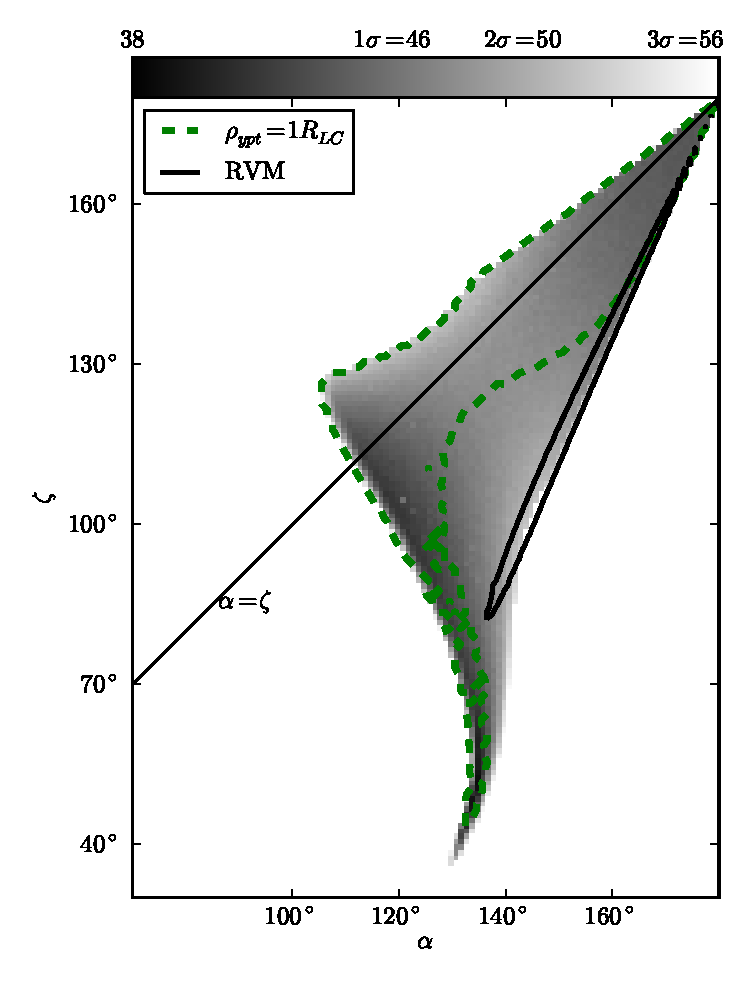
\includegraphics[scale=.8]{chapters/multiWaveLength/figures/J1513-5908Map.eps}
\caption[Map of $\chi^{2}$ for PSR J1513-5908 fit to radio polarization in the $\alpha$-$\zeta$ plane]{\label{fig:J1513-5908Map}Figure taken from \cite{hartogJ1513}.
Map of $\chi^{2}$ for PSR J1513-5908 fit to radio polarization in the $\alpha$-$\zeta$ plane.
Overlaid are  $3\sigma$ above $\chi^2_{\rm min}$ contour for
zero altitude RVM fit (black) and $3\sigma$ above $\chi^2_{\rm min}$ contour for the assumption that emission must come from the formal open
zone.
}
\end{center}
\vskip -0.2truecm
\end{figure}

\begin{figure}[htbp]
\begin{center}
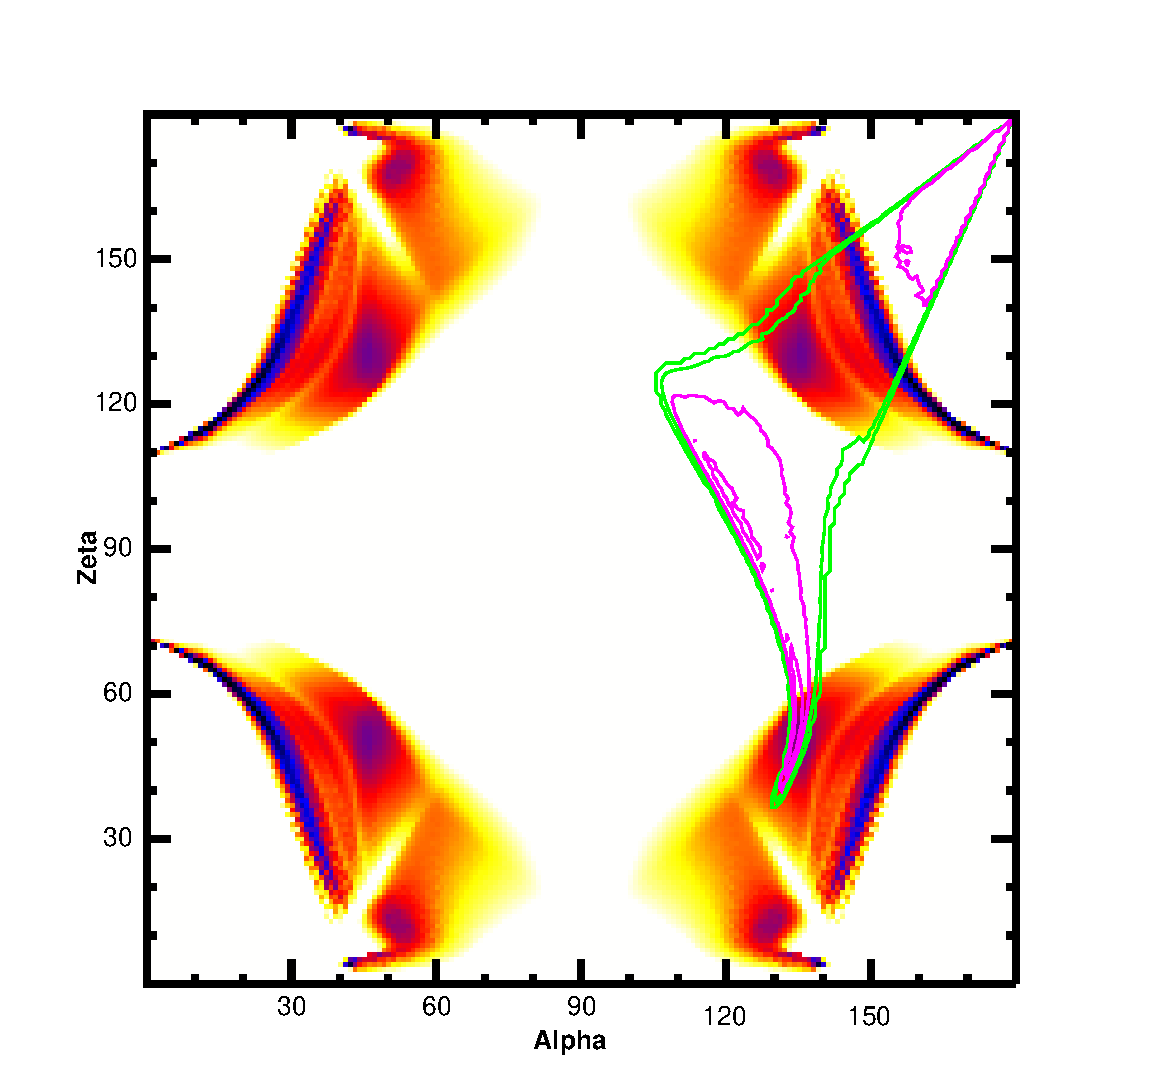
\includegraphics[scale=.8]{chapters/multiWaveLength/figures/BJ1513_w10.eps}
\caption[Pulsar geometry and emission modeling fit map of an outer gap model and radio polarization model 
for PSR J1513$-$5908 in
the $\alpha$--$\zeta$ plane of the pulsar]{\label{fig:BJ1513_w10}
Figure taken from \cite{hartogJ1513}.
Pulsar geometry and emission modeling fit map of an outer gap model 
and radio polarization model for PSR J1513$-$5908 in
the $\alpha$--$\zeta$ plane. Contours show the polarization
fit of the $0.5\sigma$ and $1.0\sigma$ regions in magenta;
and the $2.0\sigma$ and $3.0\sigma$ regions in green.
A wide range of geometries is allowed by these polarization data,
including the best $\gamma$-ray fits. Good fits must also match the
phase of the magnetic dipole axis (see text).
}
\end{center}
\vskip -0.2truecm
\end{figure}

\begin{figure}[htbp]
\begin{center}
\includegraphics[width=\textwidth]{chapters/multiWaveLength/figures/J1513_lc.eps}
\caption[Radio and $\gamma$-ray light curves of PSR J1513$-$5908 with model light curve for $\alpha=153^\circ$, $\zeta=133^\circ$]{\label{fig:J1513_lc}
Figure taken from \cite{hartogJ1513}.
Radio and $\gamma$-ray light curves of PSR J1513$-$5908 with model light curve for $\alpha=153^\circ$, $\zeta=133^\circ$.
A single
peak dominates since the line of sight skims the $\gamma$-ray caustic. The
radio emission altitude is 0.24$R_{\rm LC}$ and polarization and
$\gamma$-ray fits both indicate that the magnetic axis (green upwards arrow)
leads the radio peak by $\phi=0.08$.
}
\end{center}
\vskip -0.2truecm
\end{figure}



The paper ``Broad-Band KeV to MeV Characteristics of Soft $\gamma$-Ray Pulsar PSR J1513$-$5908''
\citep{hartogJ1513} aims to do a 
spectral study covering 2 KeV to 1 GeV including 
updated {\it Fermi} data and revisited archival RXTE-PCA and HEXTE data
along with historic CGRO-COMPTEL data of the pulsar PSR J1513$-$5908 (PSR B1509$-$58).
The pulsar was also analyzed using radio polarization data.

The polarization data analyzed is 1.4 GHz data.
The pulsar PSR J1513$-$5908 has a period of 151 ms.
Also noted in the paper is
an extra component in the radio intensity of PSR J1513$-$5908
before the peak of the main pulse.
We had hoped to model this component using polarization
but the scatter of the data was too large to derive
useful fit results.

The typical retarded dipole with photons projected tangent to the magnetic
field lines is used to calculate the position 
angles of the polarization.  Further, models used here
extrapolate from the classical RVM allowing emission from finite
radial altitudes above the surface of the neutron star with relativistic and sweep-back effects.  
Allowed altitudes ranged between
$.002R_{\rm{LC}}$ (the radius of the neutron star assuming $R_{\rm{NS}}\sim 15$ km) to $.9R_{\rm{LC}}$.

Figure~\ref{fig:intAndPAJ1513alpha153zeta133} shows the polarization position angle sweep and intensity
profile for 20 cm data.  The sweep is relatively simple and shows no signs of orthogonal
mode jumps or multiple altitude.  RVM fits relatively well to the polarization with
$\chi^2_{\rm{min}}=44$ for Degree of Freedom=DOF$=55-4$.  The four fit parameters are $\alpha$, the angle between
the magnetic axis and rotation axis, $\zeta$, the viewing angle as measured from the rotation
axis and the horizontal and the vertical offsets in the 
polarization angles.  The best fit model
with finite altitude has $\chi^2_{\rm{min}}=39$ for DOF$=55-5$ although the best fit model might
not be the most physically viable model as will be discussed later.  The solid red line in
Figure~\ref{fig:intAndPAJ1513alpha153zeta133} is a finite-altitude model at $\alpha=153^\circ$,
$\zeta=133^\circ$, and $R=0.24R_{\rm{LC}}$ with $\chi^2=48$.  Green circles on the
solid red line mark the expected end of emission based on a formal open zone assumption.


Figure~\ref{fig:J1513-5908Map} shows the best fit $\chi^2$ surface map projection in the
$\alpha$-$\zeta$ plane for the single-altitude model.  
The $3\sigma$ contours for the RVM fit are
overlaid on the color map in black.  Additionally, on this panel is a green contour that
encloses the model parameters for which model emission phase is equal to or greater than
the emission phase seen in the data.  The model emission phase is defined by the emission
from the classic open field lines.  Overlap between these contours is minimal.  This indicates
a physical need to increase emission phase from RVM either by increasing the altitude of emission
or widen the open zone cap.

Following \cite{romani2010constraining} we fit the $\gamma$-ray
light curve using the $\chi_3$ statistic. While PSR J1513$-$5958 is
very energetic, implying a small gap and emission close to the last closed
field lines, we find appreciably better light curves for a modest gap width,
$w=0.05-0.1$. In Figure~\ref{fig:BJ1513_w10}, the background color scale shows the goodness of
fit for an outer gap  model with $w=0.1$. Overlaid are
contours from the radio fitting. To be a viable model, the $\gamma$-ray fit
must lie inside the radio contours. Since the polarization presents a simple sweep, this
is not very constraining, with a wide range of geometries compatible at the
$3\sigma$ level. However, the polarization fit also tightly constrains
the phase of the magnetic axis relative to the radio intensity peak. For
a viable model, this should match as well.

The strip of best $\gamma$-ray fits crosses the radio-allowed region
along $\alpha=153^\circ$ and $\zeta=145^\circ$ to 
$\alpha=156^\circ$ and $\zeta=128^\circ$
with $\chi_3<4.5$. In
this region the phase of the magnetic axis ranges from $-0.06$ to $-0.08$
(in fractions of a period)
and the radio emission altitude varies from $0.1$ to $0.3R_{\rm LC}$.
In Figure~\ref{fig:J1513_lc}, we show the fit $\gamma$-ray light curve 
for $\alpha=153^\circ$ and $\zeta=133^\circ$.
The radio fit altitude is $0.24R_{\rm LC}$ and the polarization
fit is $1.2\sigma$ from its minimum. In this region {\it both}
the $\gamma$-ray and polarization fits place the magnetic dipole axis
0.08 before the radio peak.  A second region of plausible $\gamma$-ray fits
(with $\chi_3 \approx 5.4$) lies close to the polarization fit minimum.
In this region, $\alpha=135^\circ$ and $\zeta=51^\circ$ 
and the $\gamma$-ray light curve, while
dominated by a single peak, has a tail to phase $0.5$.  However the fit magnetic
axis phases do not agree (-0.03 for $\gamma$-ray, 0 for radio) and the radio
altitude is quite high, 0.75 to 0.85$R_{\rm LC}$. At this altitude the details
of the magnetic structure are less reliable; so we prefer the lower altitude
solution with the correct phase match. At this lower altitude, there is
also room for the field lines to open within the light cylinder, giving
a y-point radius $<1$ and a larger effective $w$.


\section{PSR J0737$-$3039A: Characterizing a Double Pulsar System with Finite-Altitude Model}
\paperref{This section is based on work done for ``\it{Fermi} LAT Pulsed
Detection of PSR J0737$-$3039A in the Double Pulsar System'' \citep{guillemot2013fermi}.}

\begin{figure*}[t!!]
\begin{center}
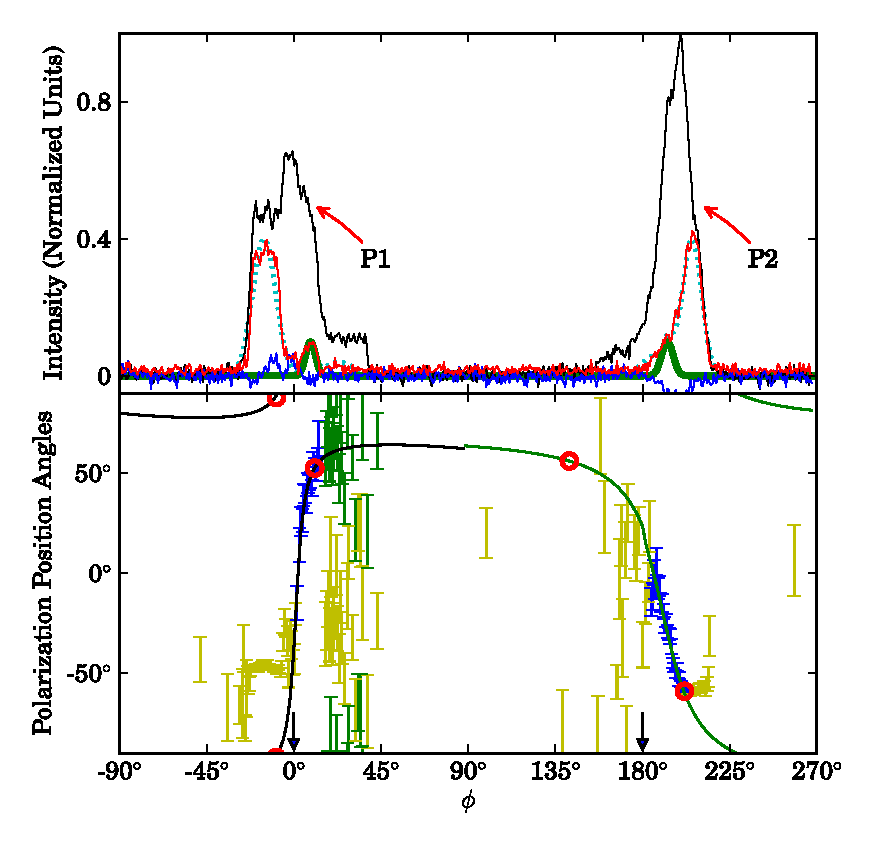
\includegraphics[width=0.9\textwidth]{chapters/multiWaveLength/figures/figure3-0737.eps}
\caption[Polarimetric profile for PSR J$0737-3039$A as observed at 1.4 GHz
with the Parkes radio telescope]{
Figure taken from \cite{guillemot2013fermi}.
Polarimetric profile for PSR J$0737-3039$A as observed at 1.4 GHz
with the Parkes radio telescope (R.~N.~Manchester, private communication). Top panel:
Stokes parameter curves (black is total intensity, red is linear polarized intensity, and
blue is circularly polarized intensity) and Gaussian decomposition
of the linear intensity components (dotted curve is all linear and the thick green
curve gives the rapid sweep central component fit here). Bottom: position angle
data (blue: central components, yellow: other position angle values, green: P1 tail with
an orthogonal mode jump). The smooth curves give the best fit model for the two
poles while the red circles denote the boundaries of the open zone at the
emission altitude. Arrows denote the phase of the closest approach of the
magnetic axes to the Earth line-of-sight.
\label{fig:polarfit}} \end{center}
\vskip -.3truecm
\end{figure*}


\begin{figure*}[t!!]
\begin{center}
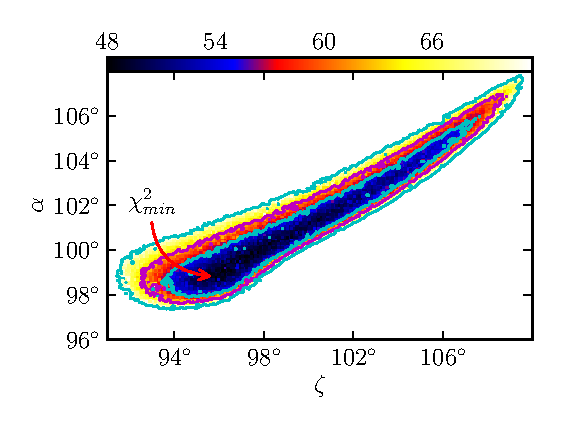
\includegraphics[width=0.9\textwidth]{chapters/multiWaveLength/figures/figure4-0737.eps}
\caption[Map of $\chi^2$ surface of the RVM fit to the radio polarization data
(central components) for PSR J$0737-3039$A in the $\alpha$--$\zeta$
plane]{Figure taken from \cite{guillemot2013fermi}. Map of $\chi^2$
surface of the RVM fit to the radio polarization data (central components) for
PSR J$0737-3039$A in the $\alpha$--$\zeta$ plane. The best fit orientation
angles ($\alpha,\, \zeta$) are indicated by an arrow, while the contours are
shown at the $1\sigma$, $2\sigma$ and $3\sigma$ levels above $\chi^2_{\rm min}$.\label{fig:polarchisq}}
\end{center}
\vskip -.3truecm
\end{figure*}


\begin{figure*}[htbp]
\begin{center}
\includegraphics[width=0.9\textwidth]{chapters/multiWaveLength/figures/figure5-0737.eps}
\caption[Light curves for PSR J$0737-3039$A at the $\alpha$ and $\zeta$ angles determined 
from the radio polarization study]{Figure taken from \cite{guillemot2013fermi}.
Light curves for PSR J$0737-3039$A at the $\alpha$ and $\zeta$ angles determined
from the radio polarization study, and for the outer gap model (solid blue line) and the
two-pole caustic model (dashed green line). The observed radio and $\gamma$-ray profiles are
shown as a solid red line and as a shaded gray histogram, respectively. See
Figure~\ref{fig:polarfit} for the definition of the magnetic axis phase
$\phi_B$. The blue arrow denotes the location of the magnetic axis under the outer gap
and two-pole caustic geometries. \label{fig:lcmodeling2}} \end{center}
\vskip -.3truecm
\end{figure*}


\begin{table*}
\caption{Polarization Fit Parameters for PSR J$0737-3039$A
\label{tab:polarfitpars}}
        \begin{center}{\small
        \def\arraystretch{1.5}
	\begin{tabular}{llllll}
        \hline
$\alpha$ $(^{\circ})$ & $\zeta$ $(^{\circ})$ & $R_{1}/R_{\rm LC}$ & $R_{2}/R_{\rm LC}$ & $\chi^{2}$ & DOF
\\ \hline
${98.8}^{+8}_{-1.5}$ & ${95.8}^{+13.2}_{-4.3}$ & $0.01^{+0.22}_{-0.01}$ & $0.11^{+0.49}_{-0.05}$ & $48$ & $35$
\\ \hline
        \end{tabular}}
\tablecomments{Errors are the extrema of the $1\sigma$ contours in the full
multidimensional parameter space. $R_{1}$ is the emission altitude of the
central component of P1 and $R_{2}$ is the altitude of the central component of
P2.} \end{center}
        \end{table*}




The paper \citep{guillemot2013fermi} reports the detection of 
PSR J0737$-$3039A, the first detection of
a mildly recycled pulsar by the {\it Fermi} Large Area Telescope.  
Such a pulsar is only mildly spun up by its companion.
The pulsar PSR J0737$-$3039A
is in a 2.4 hour orbit with another pulsar
\citep{burgay2003increased,lyne2004double}.
Such a detection is exciting
because it fills in an underpopulated
region of the $P$-$\dot{P}$ picture
\citep{psrcat}.

Further,  understanding the pulsars formation has been 
of interest.
The viewing angle is a measure of the misalignment
between the spin axis and orbital angular momentum
since the inclination of the binary system is 
known.  This measurement in turn is given as $\zeta$
near $90^\circ$ (as discussed below) indicating 
that the misalignment angle is small.
This has important implications on the formation
theory of the system 
\citep{breton2008relativistic,ferdman2013double,podsiadlowski2005double}.

The 1.4 GHz data from Parkes radio telescope was
used in the analysis of 
PSR J0737$-$3039A.
We used orthogonal mode jumps and interstellar
scattering as well as multiple and finite altitude.
We fit only the central components of the two peaks. 
We believed that the trailing edges of
the emission was dominated by plasma effects
and that the present model would not adequately 
capture the field line structure from 
this much higher emission.  Thus we 
favored modeling only the central part
of the polarization of the two radio peaks.
In particular, the flattened components of 
the polarization can not be modeled using
typical magnetic field lines and single altitudes.  
 
Figure~\ref{fig:polarfit} labels the  
Gaussian components used for the intensity 
in the upper panel (green thick line) and the polarization in
the lower panel (blue data points).  
The unmodeled data points are in yellow on
the Figure~\ref{fig:polarfit}.
Trailing edges of $P1$ in linear intensity
are separated from the central component
by linear intensity of zero which suggests
a orthogonal mode jump (for a more in depth 
discussion of this phenomena see Section \ref{sec:MAISOM}). 
The green data points show the
polarization offset by 90$^\circ$.

The black and green solid lines on the lower
panel of Figure~\ref{fig:polarfit} are the best fit model
to the blue polarization data points.
The altitudes for the two components are
different at $0.01R_{\rm{LC}}$ for $P1$ and 
$0.11R_{\rm{LC}}$ for $P2$.  At these altitudes,
The red circles indicate the open zone 
phase expected.  Interestingly, the polarization
not modeled falls outside of this phase, indicating
that the polarization is from higher altitude emission
or from emission within the formal closed zone and hinting
at reasons for its unusual structure.  Indeed, our model is
then one where the central components are from the center
of a hollow cone of emission where the altitude is relatively low
and the wings are from the higher altitudes of the cone.
Full fit parameters and errors are given in Table \ref{tab:polarfitpars}.
The fit map of $\chi^2$ is given in Figure~\ref{fig:polarchisq}.

The results of the polarization fitting were compared to 
$\gamma$-ray light curve modeling results.  Namely,
the polarization fitting produced a phase of closest approach for 
the surface dipole axis.  Both outer gap and two-pole caustic
models produced acceptable light curves in the region
of best fit in the radio polarization as seen in
Figure~\ref{fig:lcmodeling2}.  But the 
model phase zero ($\phi=0$) of the radio and $\gamma$-ray is offset by
$0.1$.  One possible explanation is the lack of 
plasma effects in the modeling.  
For instance, \cite{kalapotharakos2012gamma}
found that including finite conductivity in
magnetohydrodynamics simulations will cause such
a lag compared to vacuum models.

In addition to polarization modeling,
simultaneous fits in radio and $\gamma$-ray
to the light curves
was also performed resulting in
similar geometric angle constrains.


\section{Population Study: Characterizing Sub-luminous $\gamma$-Ray Pulsars Using Polarization}
\paperref{This section is based on work done for
``Sub-luminous $\gamma$-Ray Pulsars''
\citep{romani2011sub}}


In the paper ``Sub-luminous $\gamma$-Ray Pulsars'' \citep{romani2011sub} we aimed
to show that pulsars sub-luminous in the $\gamma$-rays
is due to alignment using radio polarization modeling
and data.
The $\gamma$-ray luminosities scales with the spin-down energy as
$L_{\gamma}\approx(\dot{E}\times 10^{33} $ erg/s$)^{1/2}$.
This is based on properties of the Goldreich-Julian model
($L_{\gamma}\propto\dot{E}^{1/2}$, see, for example, \cite{lyne2006pulsar})
plus observation of pulsars \citep{psrcat}.
However, a number of pulsars have luminosity or limits 
that are more than an order of magnitude below this
estimated luminosity, $L_{\gamma}$.
The paper aims to test whether this weak luminosity 
is due to the pulsars beaming away from the Earth.
Other explanations include the pulsars having physical
properties that causes low luminosity or the estimated distance
to the pulsars is drastically off and they are farther away 
than calculated.

\begin{figure}[t!!]
\begin{center}
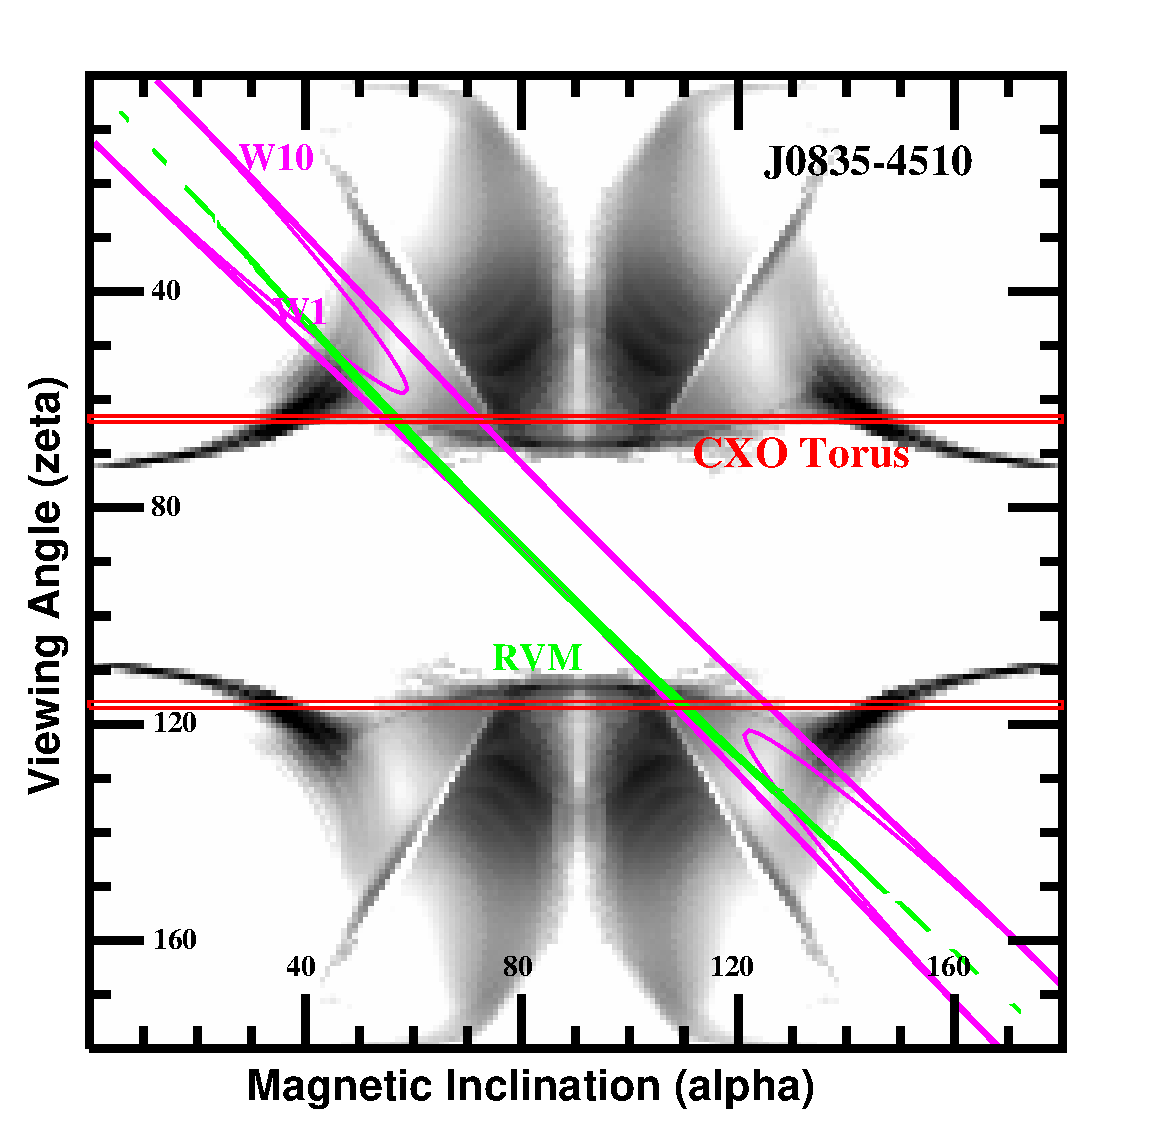
\includegraphics[width=0.5\textwidth]{chapters/multiWaveLength/figures/f2.eps}
\caption[The $\gamma$-ray fit map for Vela in the $\alpha$--$\zeta$ plane with radio polarization, X-ray torus, and pulse width constraints]{
\label{VelaEx} 
Figure taken from \cite{romani2011sub}.
The $\gamma$-ray fit map for Vela in the $\alpha$--$\zeta$ plane with radio polarization, X-ray torus, and pulse width constraints.
The background gray scale shows the goodness of fit of the {\it Fermi} light curve to a
basic outer gap model, with dark colors being better fits. Additionally, red lines mark
constraints from an X-ray pulsar wind nebula torus fit, green contours mark constraints
from RVM, and magenta contours mark constraints from opening angle arguments.
}
\end{center}
\end{figure}


\begin{figure}[htbp]
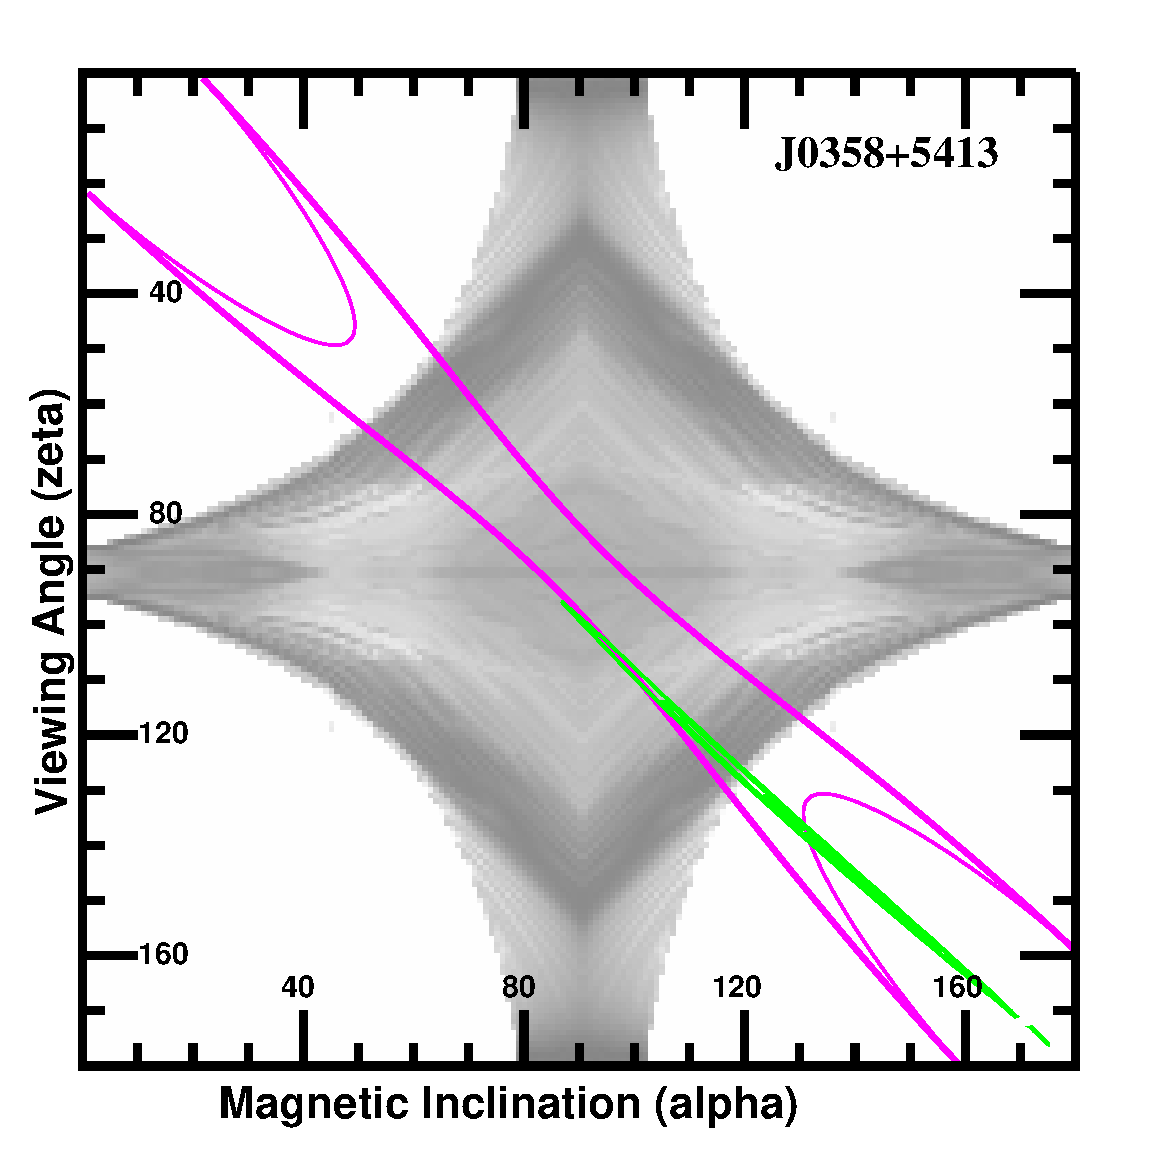
\includegraphics[width=0.5\textwidth]{chapters/multiWaveLength/figures/f3cor_a.eps}
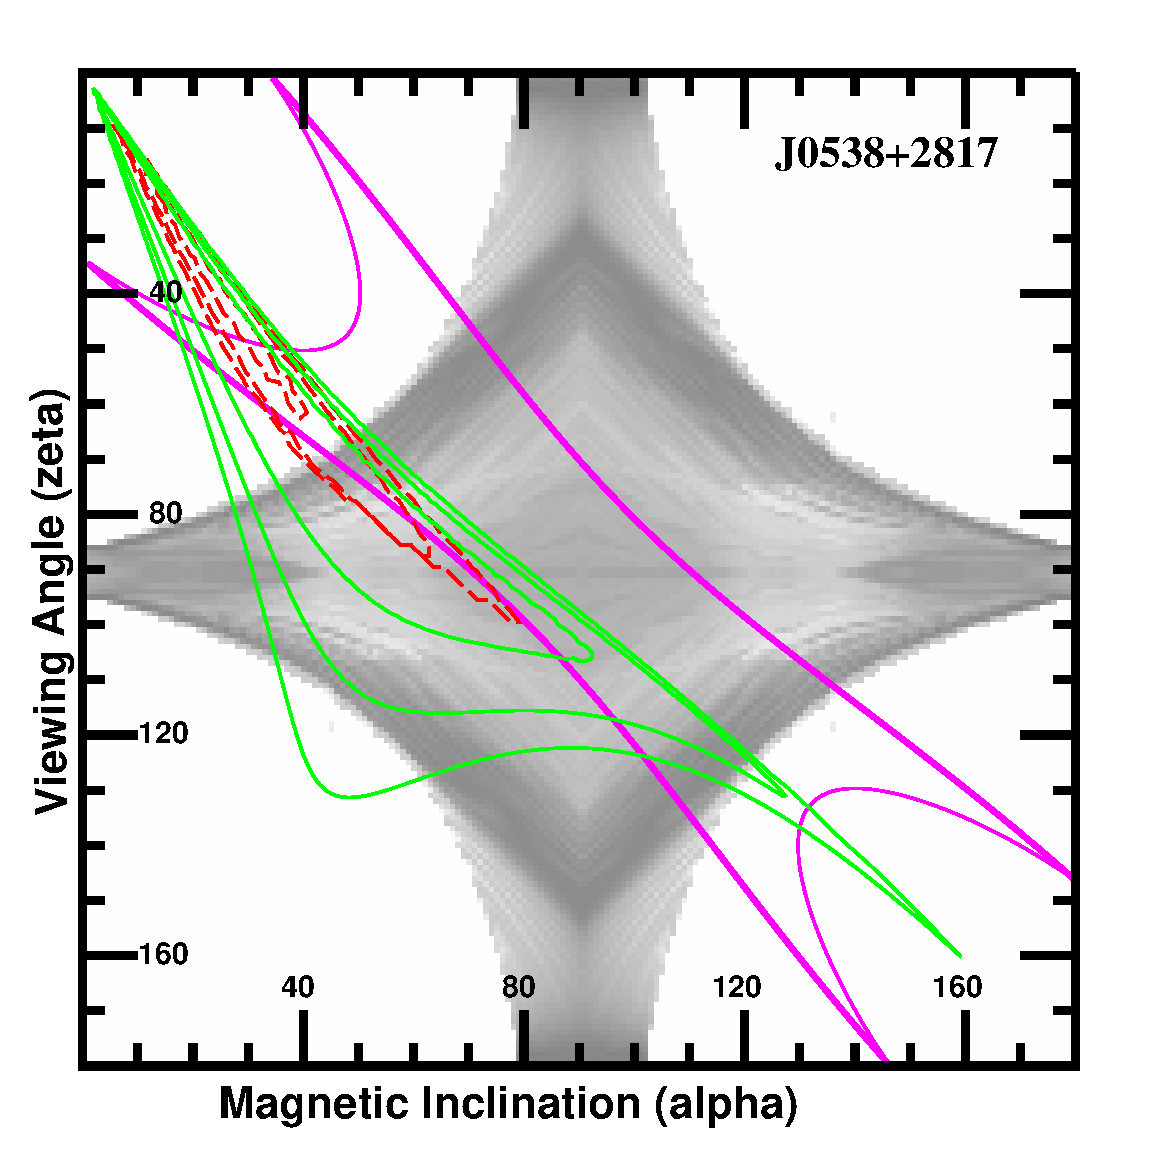
\includegraphics[width=0.5\textwidth]{chapters/multiWaveLength/figures/f3cor_b.eps}
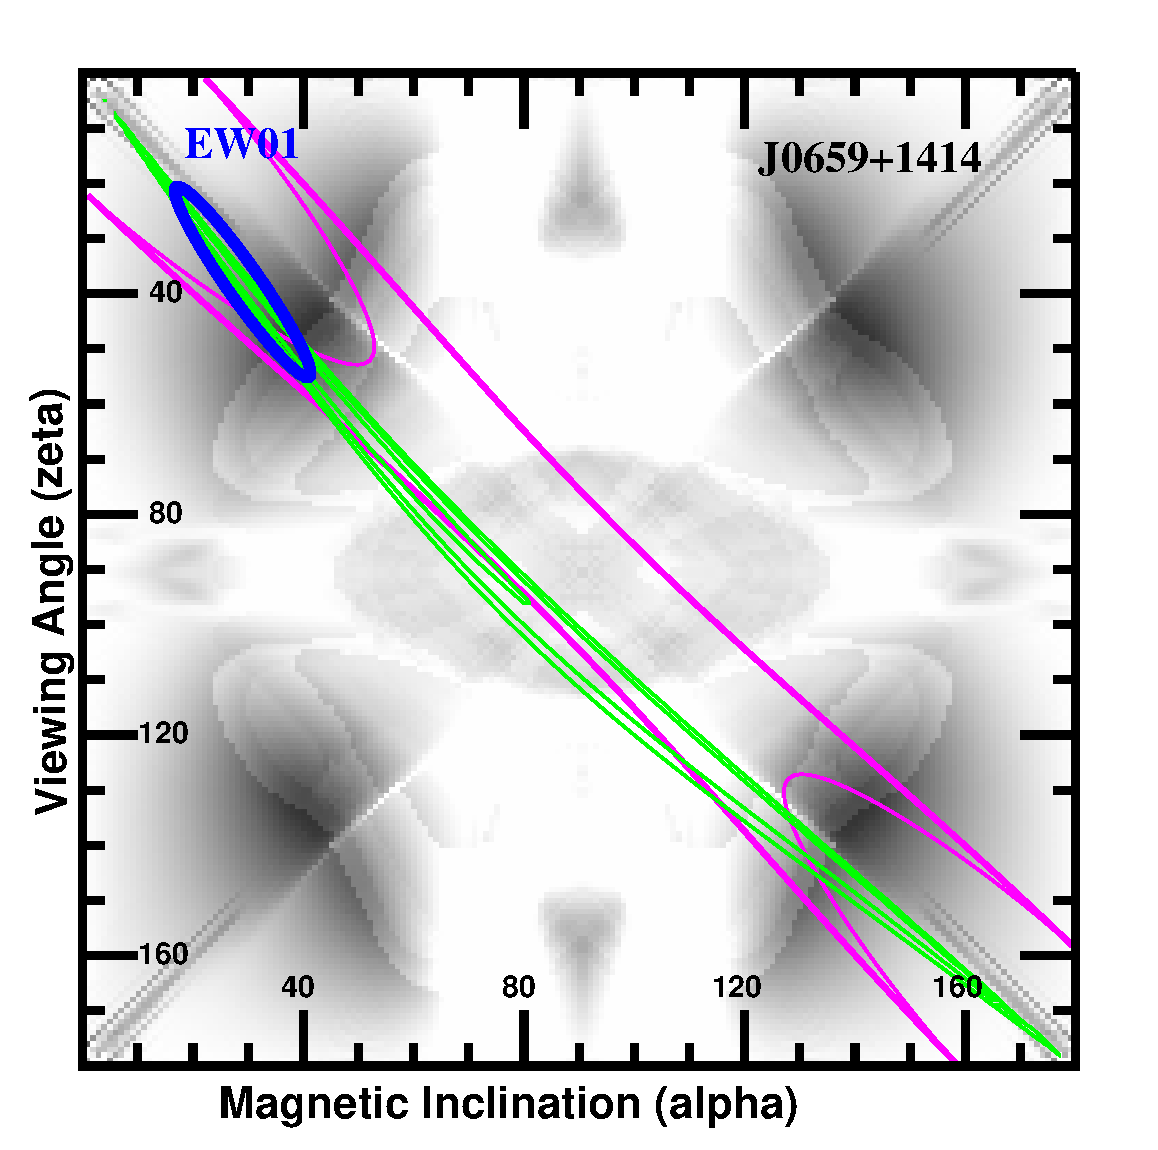
\includegraphics[width=0.5\textwidth]{chapters/multiWaveLength/figures/f3cor_c.eps}
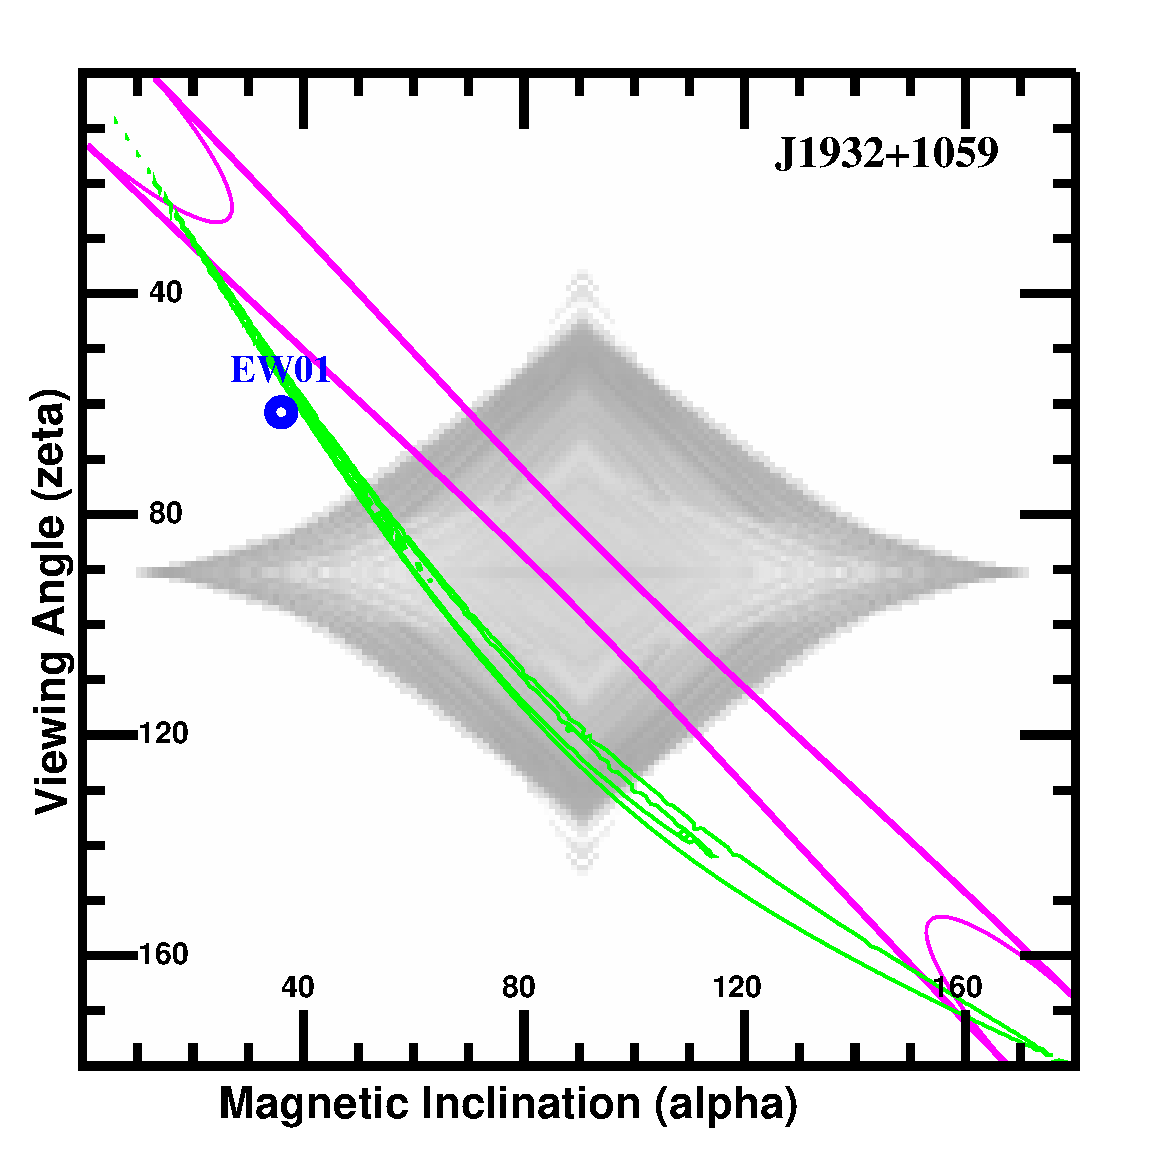
\includegraphics[width=0.5\textwidth]{chapters/multiWaveLength/figures/f3cor_d.eps}
\caption[The $\gamma$-ray fit map for sub-luminous pulsars with parallax
distances in the $\alpha$--$\zeta$ plane with radio polarization and pulse
width constraints]{ \label{plx_const} 
Figure taken from \cite{romani2011sub}.
The $\gamma$-ray fit map for sub-luminous pulsars with parallax 
distances in the $\alpha$--$\zeta$ plane with radio polarization and pulse
width constraints.
The backgrounds show the generic locations providing
sharp outer gap pulses, except for PSR J0659$+$1414, where the background shows the
allowed fits to the observed {\it Fermi} pulses, including lower altitude 
(two-pole caustic model)
%Pole Caustic TPC, Dyks \& Rudak 2003)
emission. 
``Good'' fits here for the other pulsars are in white regions because
of the sub-luminous nature of the pulsars.
Three green contours show the loci of best RVM matches, while the
bold and narrow magenta curves showed the regions allowed by emission from
the static dipole open zone for our estimated emission altitude. For PSR J0659$+$1414 (PSR B0656$+$14)
and PSR J1932$+$1059 (PSR B1929$+$10) the RVM fits of \citet{everett2001emission} are indicated.
For PSR J0538$+$2817 the fits imply large emission altitudes, requiring
a numerical magnetosphere model. The fits to the polarization geometry using
such models are shown by the dashed (red) contours.
}
\end{figure}

\begin{figure}[t!!]
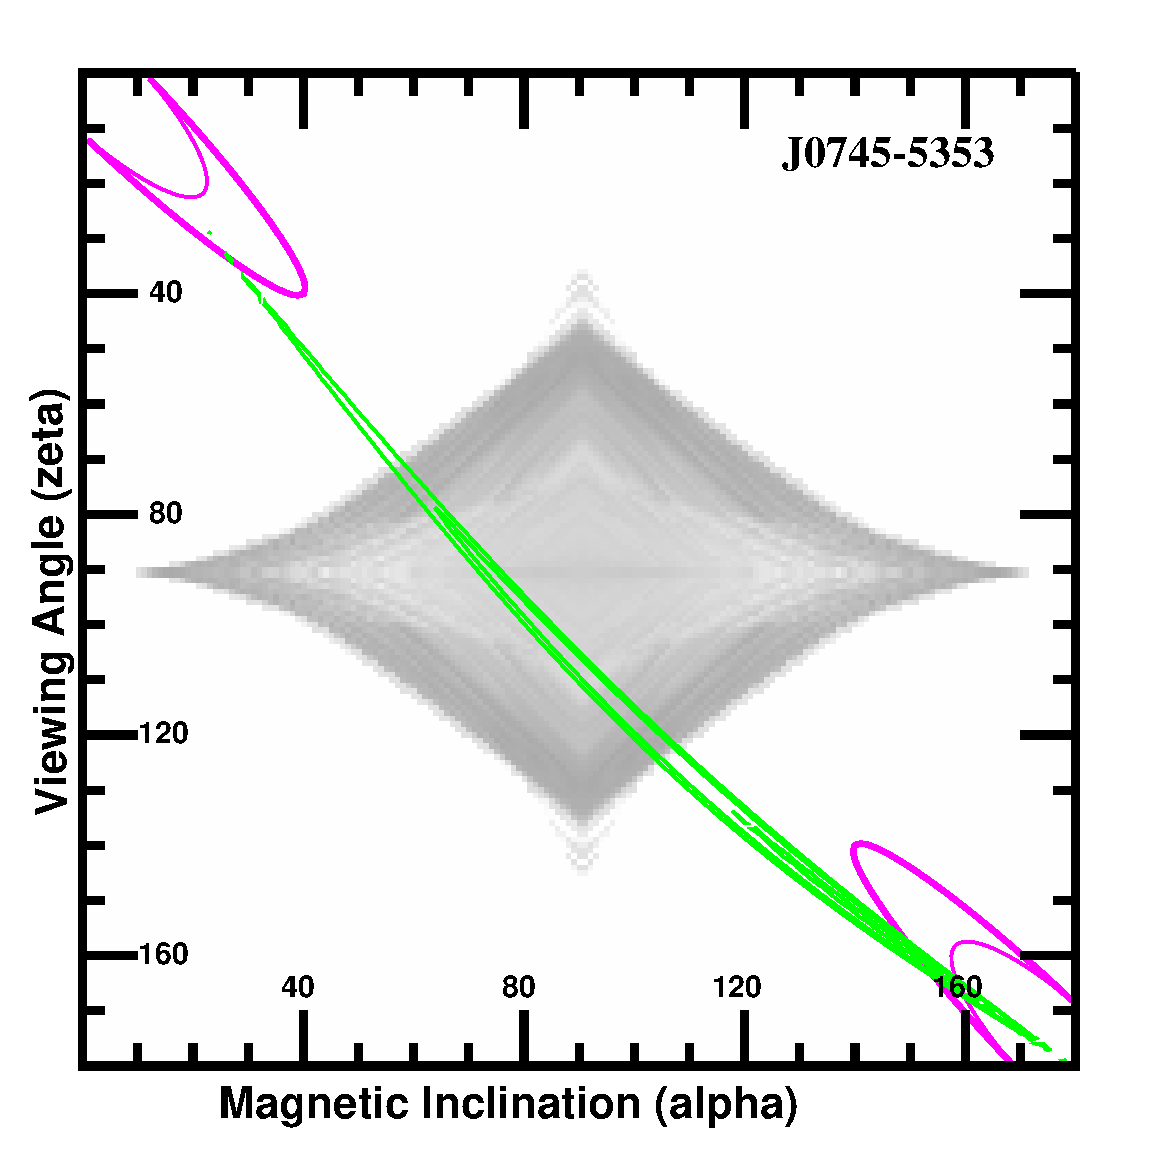
\includegraphics[width=0.5\textwidth]{chapters/multiWaveLength/figures/f4cor_a.eps}
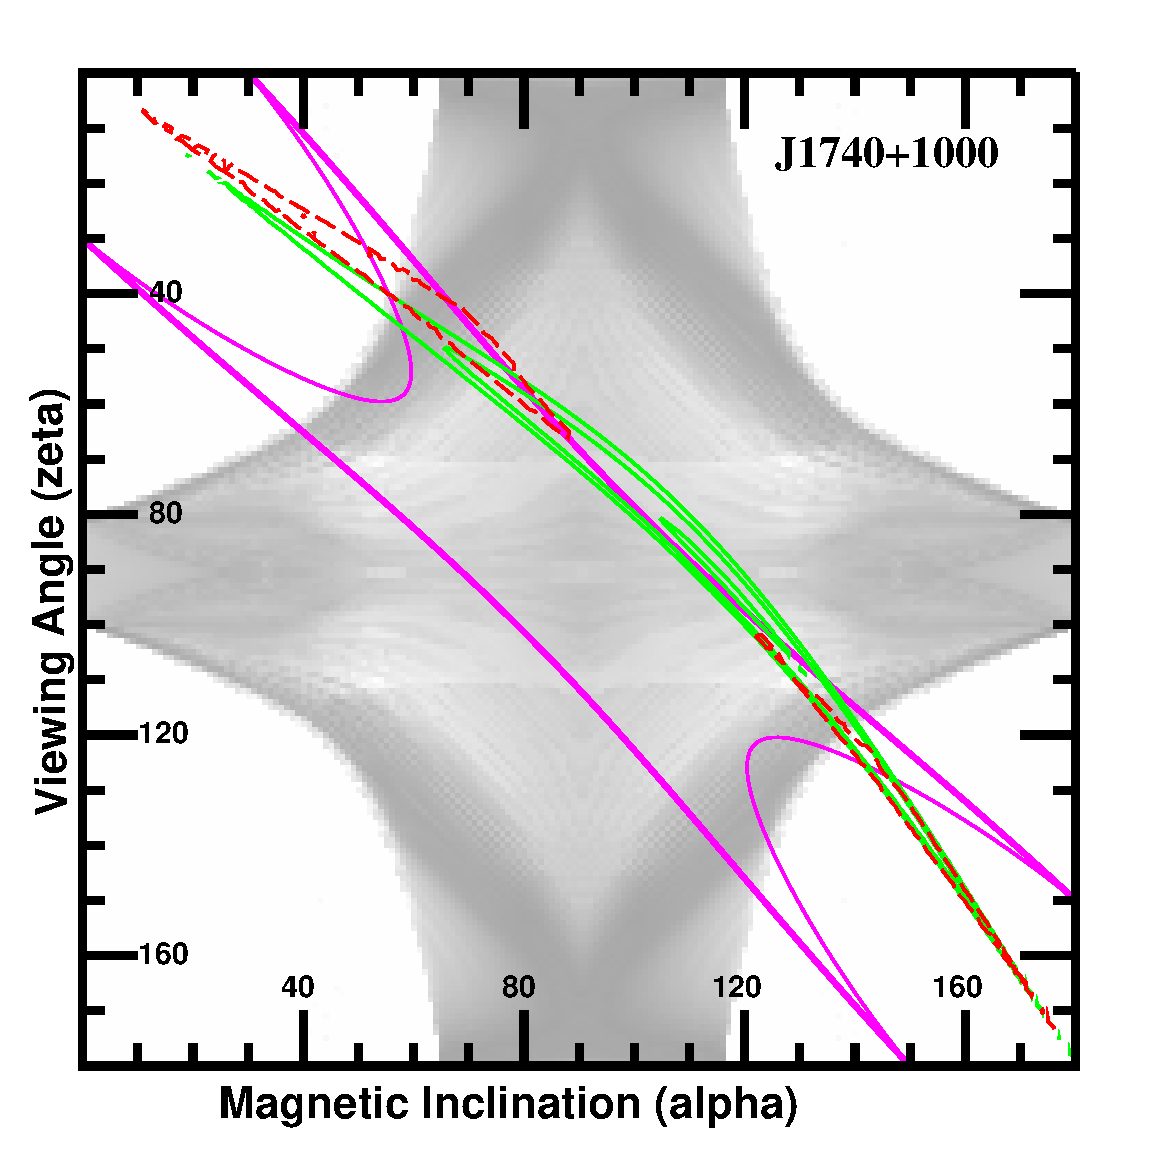
\includegraphics[width=0.5\textwidth]{chapters/multiWaveLength/figures/f4cor_b.eps}
\caption[The $\gamma$-ray fit map for sub-luminous pulsars without parallax 
distances in the $\alpha$--$\zeta$ plane with radio polarization and pulse
width constraints]{\label{noplx_const} 
Figure taken from \cite{romani2011sub}.
The $\gamma$-ray fit map for sub-luminous pulsars without parallax
distances in the $\alpha$--$\zeta$ plane with radio polarization and pulse
width constraints. For geometries
away from the gray background, the sources are not expected to have strong 
outer magnetosphere $\gamma$-ray pulses. 
``Good'' fits here are in white regions because
of the sub-luminous nature of the pulsars.
The PSR J1740$+$1000 data suggest large
emission altitude requiring numerical modeling; the locus of best fits for these models 
is shown by the dashed (red) contours.
}
\end{figure}
Open zone arguments are utilized 
in this paper to constrain acceptable parameter space.  
The parameters $W_1$ and $W_{10}$ represent the
width of the radio pulse assuming that the pulse
ends when the intensity falls below $1\%$ or $10\%$
respectively.  If one definition is more appropriate
for a given pulsar, it will be noted below.
For more details on the relationship between
the phase width and the size of the open zone, 
see Section \ref{sec:beamingGeometry}.

Figure~\ref{VelaEx} is an
example of the use of 
multi-wavelength data to strongly 
constrain the geometry of 
a pulsar.  
The pulsar modeled here is the Vela pulsar (PSR B0833$-$45 or PSR J0835$-$4510).
The pulsar is modeled with $\gamma$-ray data,
radio polarization data, opening angle constraints as
well as X-ray pulsar wind nebula torus fitting 
(see Section \ref{subsec:ToriModeling}).
multi-wavelength data of Vela is used to strongly restricts the possible
parameter space and similar modeling is done for the sub-luminous pulsars.
The magenta contours represent limits
imposed by beaming geometry.  Thin magenta lines represent
$W_{1}$ constant where models with a pulse width
that would accommodate the data are in either corner of the
fitting plane.  For the $W_{10}$ constraint, the models
are limited to those within the thick magenta lines.
The green and red contours show the lowest $\chi^2$ regions
for polarization model fitting.

Unfortunately, none of the other pulsars have clear 
X-ray pulsar wind nebula tori which are strong constraints
on the parameter space.
Four of the pulsars analyzed using polarization have parallax distances available
(PSR J0358$+$5413, PSR J0538$+$2817, PSR J0659$+$1414, and PSR J1932$+$1059) 
and two do not have parallax distances available (PSR J0745$-$5353 and PSR J1740$+$1000).
The fit maps of Figures~\ref{plx_const} and~\ref{noplx_const} show
regions with $\gamma$-ray model gap width of $w\approx L_{\gamma}/\dot{E}$.
The grey background is the fit map of the $\gamma$-ray model to 
a generic single peak pulse except for PSR J0659$+$1414 for which $\gamma$-ray data is
available.  The darker the region, the better the fit.  
Note though that because the pulsars are sub-luminous, the best fit regions
are those that are white regions, since no $\gamma$-rays are present
for these models. 
Blue contours are polarization fit
regions from the literature.  

In the fitting results of PSR J0358$+$5413, the RVM favored $\alpha>110^\circ$.
Additionally, with $W_1$ constraint, $\alpha>130^\circ$ and $\zeta>140^\circ$.
The $W_{10}$ constraints are not more restrictive than the RVM fitting
results.
The pulsar PSR J0358$+$5413 could be sub-luminous but 
some non-sub-luminous geometries are also plausible.

For PSR J0538$+$2817,
the acceptable parameter space given by the
RVM fit is rather large as can be seen in 
Figure~\ref{plx_const}.  However, the combination
of the RVM contours and the $W_{1}$ and $W_{10}$ constraints
are much more restrictive.  With the $W_{1}$ constraint,
the possible models are confined to $\alpha<35^\circ$
and $\zeta<50^\circ$.  The numerical finite-altitude 
fits are included for this pulsar
on the figure in red dashed contours.  These fits
again favor smaller $\alpha$ and $\zeta$ where
one would not expect outer gap emission in $\gamma$-rays.
In contrast, the jet-like feature of the X-ray pulsar
wind nebula does suggest $\zeta\approx90^\circ$
but are too faint to do a formal fit with the torus model
\citep{romani2003pulsar,ng2007origin}.


PSR J0659$+$1414 was previously studied in the radio polarization
\citep{lyne1988shape,everett2001emission,weltevrede2010gamma} 
and the results of \cite{everett2001emission} are included in blue
on the figure.  In our fits to RVM, the model favored $\alpha<80^\circ$
but the pulsar has extended emission well beyond the main peak
such that including the $W_1$ restriction gives $\alpha<35^\circ$.
The goodness of fit given in the figure is for a two-pole caustic
$\gamma$-ray model fit to the {\it Fermi} Large Area Telescope data
available for this pulsar. 
The outer gap model emission best fits are restricted
to $50^\circ<\alpha<130^\circ$ and are well beyond the restrictions
of the strongly extended emission seen in this pulsar.  

The fitting of the polarization data of PSR J1932$+$1059 prefers 
$\alpha<60^\circ$.  However, the additional constraints of 
$W_{10}$ prefers $\alpha<20^\circ$ and $W_{1}$ prefers
$\alpha<15^\circ$.  The RVM fitting contour from
\cite{everett2001emission} is also included on Figure~\ref{plx_const}.
Our analysis would then imply strongly that 
this pulsar is sub-luminous through geometry 
although this pulsar
has a low $\dot{E}$ such that the $\gamma$-ray
emission may have turned off.

PSR J0745$-$5353 does not have a defined parallax distance and
thus can not be definitively categorized as sub-luminous.
From the \cite{cordes2002ne2001} model, the pulsar has a distance
of $0.25$ kpc but a distance of $7.1$ kpc from \cite{taylor1993pulsar}.
The pulsar is sub-luminous if its distance is less than $2$ kpc.
In the combined restriction of RVM and $W_{10}$, $\alpha>150^\circ$
and in the combined restriction of RVM and $W_{1}$, $\alpha>160^\circ$.
Thus if PSR J0745$-$5353 was known to be close enough for detection,
it would be a sub-luminous pulsar.

The pulsar PSR J1740$+$1000 also does not have a parallax distance but
does have a strong dispersion measure distance (Section \ref{sec:interstellarScattering}).  
Both RVM and single-altitude numerical model
fitting was performed on the radio polarization position angle data.
For $W_{10}$ and RVM modeling, $\alpha<70^\circ$ or $\alpha>120^\circ$
is preferred.
For $W_{1}$ and RVM modeling, $\alpha<50^\circ$ or $\alpha>140^\circ$
is preferred.
For $W_{1}$ and single-altitude modeling, $\alpha<30^\circ$ or $\alpha>150^\circ$
is preferred.
So although the pulsar could possibility not be detected due to 
geometry, the parameters are not restrictive enough
to test the model.

In conclusion, this paper attempted to determine whether the non-detection
of these pulsars in the $\gamma$-rays is due to beaming direction
and high altitude emission of the outer gap model.
Although the pulsars all showed evidence of being
sub-luminous due to geometry, none were ruled out
as low-level $\gamma$-ray emitters that will yet be detected
with increased {\it Fermi} Large Area Telescope exposure and pulsed searches.



\section{Conclusions}

In this chapter, several papers are reviewed which take advantage of the 
polarization data to better understand the nature of pulsars.
From the work in these papers, we can see the important role of 
the polarization modeling for radio position angle measurements. 
Both numerical models and RVM were utilized in these studies.
Often times, the rotating vector model is a helpful and easy-to-used model to
interpret
polarization when applied to suitable data.
Additionally, we see the importance of using polarization data in
connection to other wavelengths.

\chapter{Inward-Directed Photons}
\label{chapter:inwardPhotons}




\section{Exploring Inward-Directed Photon Emission Using Radio Polarization Data of PSR J1057$-$5226}

\paperref{This section is based on work done for
``Exploring Inward-Directed Photon Emission Using Radio Polarization Data of PSR J1057$-$5226''}



We apply a bidirectional model with both outward-directed photons
and inward-directed photons to understand the complex
radio polarization data of PSR J1057$-$5226 (PSR B1055$-$52).
PSR J1057$-$5226 radio polarization data matches well to
this model  when one of the
components of the polarization sweep is associated with
inward-directed photon emission.
Additionally, we discuss previous studies
of PSR J1057$-$5226 in relation to our current study
and past applications of models with inward-directed photons.
We apply $\gamma$-ray models restricted by best fit parameters
from the radio modeling.  Although possible solutions exist, results
do suggest we have not fully identified the
location of the emission within the magnetosphere with the
simplest $\gamma$-ray modeling assumptions.


\subsection{Introduction}

Pulsars have strong magnetic fields that are tied fundamentally to the
emission observed from Earth.  Charged particles follow the magnetic
field lines before emitting curvature radiation.  The projected
position angle of such radiation is a means of observing directly
the geometry of the pulsar magnetic field and is a powerful
tool for understanding the magnetosphere and the emission
mechanism of the pulsar.

A large number of pulsars have S-shaped polarization
position angle sweeps (versus phase).
A simple analytical formula which assumes the pulsar
is a vacuum point dipole
predicts these S-shaped sweeps.
This model
is called the rotating vector model (RVM, \citealp{radhakrishnan1969magnetic}).
Given the simplicity of
the model, it works surprisingly well for quite a number of
pulsar position angle data sets
(i.e. \citealp{lyne1988shape}, \citealp{phillips1990magnetic}, \citealp{everett2001emission}).

Nevertheless, for other pulsars, the polarization does not
adhere to this smooth S-shape form and has jumps and cusps that
fundamentally can not be explained using such a simple model
(i.e. \citealp{yan2011polarization}, \citealp{everett2001emission}).
Few studies have attempted to understand in-depth this difficult data but
polarization is a powerful tool for understanding
the emission of pulsars even for ``messy'' radio polarization sweeps.
Further, pulsars with complex polarization tend to be high energy
pulsars seen in the $\gamma$-rays and thus understanding these
complicated polarization sweeps will contribute to understanding 
pulsars in multi-wavelength studies (e.g. \citealp{keith2012high}).
Overall, 
developing models for this complicated
and little understood polarization
has great potential for elucidating the geometry and
emission of the pulsars.

In a previous paper (\citealp{craig2014tackling}), our aim was to build on the
simple rotating vector model (RVM).  We numerically calculated
polarization from finite altitude with and without
orthogonal mode jumps \citep{backer1976orthogonal}.
RVM accurately predicts only emission from 
the surface of the point neutron star, an altitude of zero,
because of the lack of relativistic considerations. 
The addition of finite altitude also allows for multiple-altitude
models with emission from multiple areas in the pulsar magnetosphere.
The addition of multiple altitudes explains well a number
of the jumps seen in the complex polarization data.  (A jump
in a polarization sweep for example can be seen in Figure~\ref{fig:singleAlt} 
between the polarization associated with intensity peaks $C_2$ and $C_3$.)

In \cite{craig2014tackling}, we illustrated our model by fitting 
the model to a number of pulsars.  One of these pulsars was PSR J1057$-$5226.
The polarization of the trailing component of the
$P_1$ pulse (labeled as $C_3$ in Figure~\ref{fig:singleAlt}) 
which appears to have a jump in the polarization when compared
to the rest of the sweep was not modeled.  In this current paper, this component
is treated as ``backward'' emission.
In adhering to a modified geometrically based model, this
inward-directed photon emission is calculated using the field lines of the
typical dipole but aimed in the opposite direction
of the typical outward-directed photon.  The addition of 
polarization from inward-directed photon emission is the natural next step for
a model based on geometry and guided by data.

In this current paper, we will fit the pulsar radio
polarization data and  $\gamma$-ray data and argue that
PSR J1057$-$5226 has atypical emission that makes it
a particularly interesting candidate for inward-directed photon emission.
Figure~\ref{fig:simpleFig} illustrates the configuration of 
pulsar PSR J1057$-$5226 with bidirectional photon emission.
We will discuss the formal fitting of the polarization data for PSR J1057$-$5226
in Section \ref{sec:fitting} along with fitting of the $\gamma$-ray data. 
In Section \ref{sec:intro}, we review past studies on PSR J1057$-$5226.
In Section \ref{sec:previousBidirectional}, we review
previous studies that consider bidirectional emission.

\begin{figure}[t!!]
\begin{center}
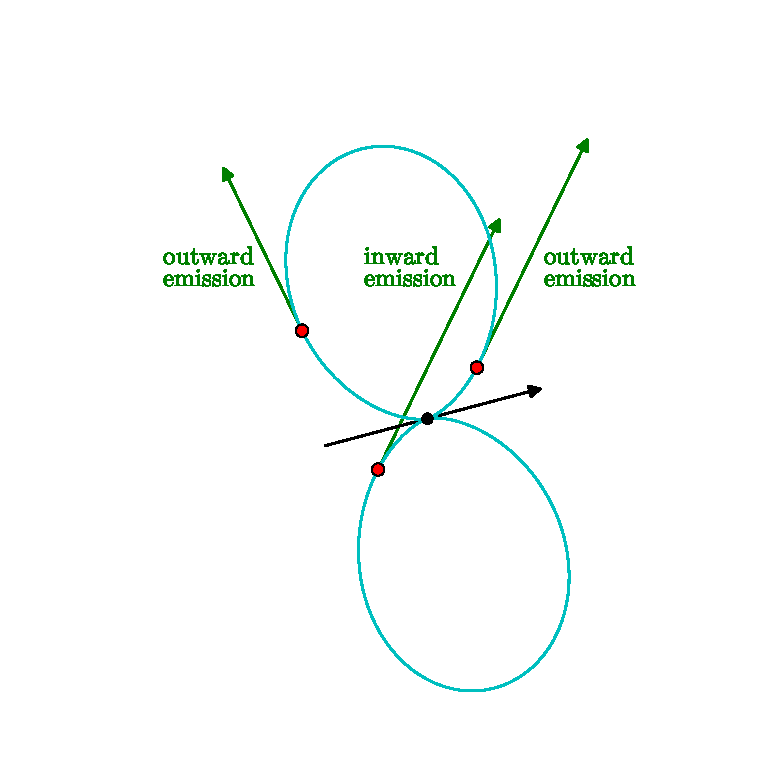
\includegraphics[scale=.8]{chapters/inwardDirectedPhotons/figures/magnetosphere.eps}
\caption[Sketch of a pulsar magnetosphere illustrating the use of inward-directed photon
emission to explain unusual polarization of PSR J1057$-$5226]{\label{fig:simpleFig}
Sketch of a pulsar magnetosphere illustrating the use of inward-directed photon
emission to explain unusual polarization of PSR J1057$-$5226. The rotation axis is
vertical. Green lines are emission from various regions of the magnetosphere
originating at red dots. Two regions emit the typical outward-directed photons
and another region emits inward-directed photons. All three arrows have the
same line of sight angle from the spin axis and thus all three will be seen by
a single observer. In terms of phase, the observer will see emission from
the ``outward'' emission on the right side of the diagram followed
quickly by the ``inward'' emission for a counter-clockwise spinning
pulsar. The pulsar will then swing around and the ``outward'' emission
on the left side of the diagram will be in the line of sight of the observer.
Thus the observer will see two pulses in the pulsar emission although one of
the pulses contains both inward-directed photons and outward-directed photons
each from a separate pole. This configuration is the one that is supported
by polarization data for PSR J1057$-$5226 and the diagram is a simplified version of Figure~\ref{fig:totDirFitPhi}.
}
\end{center}
\end{figure}



\subsection{Previous Work with PSR J1057$-$5226}
\label{sec:intro}



The pulsar PSR J1057$-$5226 (also known as PSR B1055$-$52) is a relatively young pulsar
($P=197.11$ms) with emission in the radio and $\gamma$-rays.  In radio, PSR J1057$-$5226 exhibits two
pulses with an approximate 180$^\circ$ separation in phase.  The $\gamma$-rays have been studied
using the outer gap and the two-pole caustic models (\citealp{romani2010constraining}).  
\cite{weltevrede2009mapping} have studied PSR J1057$-$5226 in radio; they applied
the RVM to the radio position angle polarization data and
applied opening angle arguments to map the polar cap emission region.  With these
models, they were forced to conclude that some emission originates from field lines outside 
the formal dipole open zone cap.  This cap is defined by field lines on the
neutron star surface that extend outside of the
light cylinder (characterized by a cylindrical distance, $R_{\rm{LC}}$, at which particles
would have to travel faster than the speed of light to co-rotate) and do not close.
They also
applied the analytic Blaskiewicz, Cordes, Wasserman (BCW, \citealp{blaskiewicz1991relativistic})
formulation to approximate different altitudes for the two pulses of 
emission.



In a previous paper (\citealp{craig2014tackling}), we applied 
a numerical geometrically-based model to an updated polarization
position angle sweep of PSR J1057$-$5226. 
Such a model 
can accurately produce polarization sweeps of much greater
heights  than the
simplistic BCW formulation. \cite{craig2012altitude}
calculated break-down altitudes to be $\sim0.05\rm{-}0.12R_{\rm{LC}}$
for BCW (depending on geometric parameters and intensity models).
The data could be modeled with emission originating mostly 
from within the open zone of the magnetosphere but at
altitudes near the formal light cylinder.  The data could
also be modeled at lower altitudes with emission originating
from well within the closed zone of the magnetosphere.

Additionally, the updated polarization position angle data used in \cite{craig2014tackling}
revealed an additional piece of polarization previously not noted in \cite{weltevrede2009mapping}.
In \cite{craig2014tackling}, we were unable to fit this piece of polarization even 
with multiple altitudes and orthogonal mode jumps (\citealp{backer1976orthogonal}).  

\cite{weltevrede2012phase}, a follow-up paper to \cite{weltevrede2009mapping}, has a 
detailed analysis of the periodic modulation of PSR J1057$-$5226. 
They found that for the $20$ period modulation, the two pulses of PSR J1057$-$5226 have a $2.5$ period phase-locked delay.
If the two pulses originate from separate poles, this delay can not be easily or simply 
explained.  Either there must be some form of communication between the poles, the emission originates
from a single pole, or some external factors are at play.
See \cite{weltevrede2012phase} for a discussion summarizing these possibilities.  


\subsection{Previous Work in Bidirectional Emission}
\label{sec:previousBidirectional}

Bidirectional emission was suggested
for pulsar radio emission in general by \cite{dyks2005reversals}.
Bidirectional emission is emission with both an outward-directed photon component
and an inward-directed photon component and is 
also called
backward or downward emission.
The inward-directed emission originates from
one pole but instead of being directed outward from the neutron star,
it is directed into the typical cone of emission and is therefore seen
at a phase that one would expect emission from the opposite
pole.  
In recent years, bidirectional emission has been suggested for 
a number of pulsars.

Figure~\ref{fig:simpleFig} offers a visual representation of bidirectional emission. In the
figure, the black arrow is the magnetic axis, the cyan loops are a pair of
field lines, and the rotation axis is vertical (not shown). The red points
represent regions where emission is produced and the green arrows represent
the path of a photon traveling tangent to the field line. All three emission
projections marked by the green arrows will be visible to a single observer
during the rotation of the pulsar. The ``outward'' emission will be
seen as the typical two pulses of the pulsar. The ``inward'' emission
will be seen near in phase to the ``outward'' emission on right side of
the diagram even though this ``inward'' emission originates from the
opposite pole.


\cite{dyks2005reversals} argued for bidirectional emission in the pulsar PSR B1822$-$09.
The interpole component of the pulsar radio profile disappears when the precursor 
component of the main pole emission appears and vice versa \citep{gil1994multifrequency}.
This behavior suggests some interpole communication or perhaps bidirectional
behavior.  In \cite{dyks2005reversals}, they estimated the radial distance of the emission
based on phase lag between the inward-directed and outward-directed photon emission assuming
both emission components come from the same region. They also estimated $\alpha$
(angle between rotation axis and magnetic axis)
based on observing both components.  Further, they argue that 
inward-directed photon emission components are more common than recognized because one does not always
see both inward-directed and outward-directed photon emission components but only the nulling of the visible 
component.

PSR B0950$+$08, PSR B1929$+$10, and PSR B0437$-$4715 were suggested to have bidirectional emission by 
\cite{dyks2005shadow}.  These three pulsars are so-called ``notched" pulsars \citep{mclaughlin2004notches}
because in radio intensity two notches of emission appear on the leading side of the main pulse,
one partially embedded in the main pulse and the other several degrees before the main
pulse.  \cite{wright2004model} argued for a model where a obscuration in the magnetosphere
along with multiple altitudes causes the double notch emission.  \cite{dyks2005shadow} created
a model where inward-directed photons are the source of this emission and the pulsar
itself is the obstruction.  In later papers however, they favor other models
to explain the double notches \citep{dyks2006model,dyks2012asymmetry}.

In \cite{weltevrede2007main}, the interaction of the two pulses of PSR B1702$-$19 is explored.  The pulsar radio intensity 
periodically brightened every 10.4 periods.  The main pulse modulation lags the interpulse modulation
by 0.43 periods.  One explanation for this phase-locked behavior is bidirectional emission where the
interpole component actually originates from inward-directed photon emission in the same region of the magnetosphere as the
outward-directed photon emission of the main pulse.  In the paper, the authors also discuss other possible explanations
such as a single wide pole.  They also discuss possible geometrical configurations needed for
bidirectional emission in PSR J1057$-$5226 and PSR B1822$-$09 based on observed
periodic intensity modulations of these pulsars.  

\cite{weltevrede2012interpole} found that the pulsar PSR J1057$-$5226 has 
a phase-locked
delay of $2.5$ periods between the pulses for the observed modulations
that occur every $20$ periods.
As pointed out in \cite{weltevrede2012interpole}, a phase-locked
delay of $2.5$ periods for the pulsar PSR J1057$-$5226 is far too long to be simply explained by the time-of-flight
delay of bidirectional emission.  But as pointed out in \cite{weltevrede2012phase}
such a delay could be caused by magnetospheric reflection or drift
(\citealp{wright2003empirical} and \citealp{melrose2012obliquely}).
We discuss this further in Section~\ref{sec:comp2012}.

\subsection{Modeling Data of PSR J1057$-$5226}
\label{sec:fitting}

\begin{figure*}[htbp]
\vskip .041\textheight
\begin{center}
%\includegraphics[width=.7\textwidth]{chapter2figures/totDirFitPhi.eps}
\special{psfile=chapters/inwardDirectedPhotons/figures/test2.eps hoffset=-145 voffset=-361 vscale=71 hscale=71}
%\special{psfile=testCloseUp.eps hoffset=-140 voffset=-395 vscale=75 hscale=75}
\begin{flushright}

\begin{overpic}[width=.66\textwidth]{chapters/inwardDirectedPhotons/figures/testCloseUp3a.eps}
\multiput(-10,30.5)(.8,-.65){30}
{\line(2,0){0.5}}
\multiput(-9.5,40.4)(.8,.44){30}
{\line(2,0){0.5}}
\end{overpic}

%\includegraphics[width=.66\textwidth]{testCloseUp2.eps}
\end{flushright}
%\special{psfile=testCloseUp.eps hoffset=100 voffset=-50 vscale=100 hscale=100}
\caption[Visualization of the pulsar model at parameters for
which $\chi^2$ is minimized assuming a single altitude of 
bidirectional emission for PSR J1057$-$5226]{
The left panel shows a visualization of the pulsar model at parameters for 
which $\chi^2$ is minimized assuming a single altitude of bidirectional emission
for PSR J1057$-$5226.  
The symbols $C_1/C_2$, $C_3$, and $P_2$ label the geometrical 
emission sites of various
polarization position angle sweep pieces 
as seen in Figure~\ref{fig:singleAlt}.
The regions $C_1/C_2$ and $P_2$ are assumed to originate
from outward-directed photons on opposite poles while
$C_3$ originates from inward-directed photons on the same pole
as $P_2$.
For this particular model
$\alpha=77^\circ$.  The cyan magnetic field lines are the last closed field
lines with $\rho_{\rm{ypt}}=0.45R_{\rm{LC}}$ and the yellow magnetic field lines are
the last closed field lines with $\rho_{\rm ypt}=1R_{\rm{LC}}$.  The red
lines and green arrows highlight regions of emission seen for $\zeta=44^\circ$
and $R_{C_1/C_2}=R_{C_3}=R_{P_2}=0.35R_{\rm{LC}}$, the best fit configuration for a single-altitude model.   The right panel is a close up of the 
pulsar with fewer magnetic field lines (yellow and cyan lines).  The transparent caps represent
regions of open field lines at $R=0.35R_{\rm{LC}}$ and $\rho_{\rm{ypt}}=0.45R_{\rm{LC}}$.
The region enclosed in the thin black line on the caps represent 
the region of open field lines with $\rho_{\rm{ypt}}=1R_{\rm{LC}}$ 
(the classical vacuum cap).  Thick curved red lines on the caps represent
regions from which we do see emission while thin curved red lines are regions
that we could see emission from for $\zeta=44^\circ$.  The rotation
axis is vertical. 
}
\label{fig:totDirFitPhi}
\end{center}
\vskip .02\textheight
\end{figure*}



\subsubsection{Fitting Procedure for Polarization Position Angle Data}
\label{sec:fitProcedure}
The model used in this paper is the same finite-altitude (measured radially from the neutron star center),
geometrically-based model as used in \cite{craig2014tackling}.
\cite{craig2014tackling} contains a more detailed description
of the model and its nuances.
The allowed range of fit altitude was  $R=R_{\rm{NS}}$ to $0.9R_{\rm{LC}}$
where $R_{\rm{NS}}$ is the neutron star radius for PSR J1057$-$5226.
The angles $\alpha$, the angle between the spin axis and
magnetic axis, and $\zeta$, the viewing angle measured from 
the spin axis were held fixed in $1^\circ$ intervals while 
all other parameters varied.  The other fit parameters
were the horizontal and vertical offsets ($\Delta \phi$ 
and $\Delta \psi$) and the altitudes ($R_{C_1/C_2}$, $R_{C_3}$, and $R_{P_2}$).
The parameters $\Delta \phi$ and $\Delta \psi$
shift the polarization position data relative to the model horizontally
and vertically.
Although these parameters contain important physical information
(the phase of closest approach of the magnetic axis and 
the absolute position angle of the magnetic axis on the
plane of the sky), they are not reported here and are treated more as 
nuisance parameters.
Additionally, phase of zero in the radio polarization
model is the same as phase of zero in the $\gamma$-ray model
(see Section \ref{sec:gam}).
The altitudes are measured radially from the center of the pulsar and
are the distance at which photons are emitted tangent to the magnetic 
field lines.  The magnetic field line structure used here is 
that of a relativistic rotating point dipole given in \cite{kaburaki1980determination}.
A simulated annealing scheme was used to minimize
$\chi^2$ \citep{flannery1992numerical} and to randomly sample
the fit parameter space within $3\sigma$  of the $\chi^2_{\rm{min}}$
and calculate fit error bars.  We also
allowed for orthogonal mode jumps.

In this paper, as in \cite{craig2014tackling}, we use the parameter
$\rho_{\rm{ypt}}$.  This parameter is the cylindrical distance
required of the last closed field line (or the y-point)
for all emission seen in the data to originate from
open field lines. For the classical vacuum dipole 
model, $\rho_{\rm{ypt}}=1R_{\rm{LC}}$.  In terms of emission
phase, the smaller the $\rho_{\rm{ypt}}$, the more
time or phase an observer should see signal from the
pulsar for any given pulsar configuration.

We will also refer to the value $\Delta\rho=\rho_{\rm{ypt}}-\rho_{\rm{max}}$.
The value $\rho_{\rm{max}}$ is the maximum cylindrical distance 
of the model emission
from the neutron star
center (the maximum cylindrical altitude of the model;
whereas, $R_{C_1/C_2}$, $R_{C_3}$, and $R_{P_2}$ are radial distances).  

In modeling PSR J1057-5226 data, we assume that radio emission identified as $C_1$ and $C_2$ in
Figure~\ref{fig:singleAlt} originates from the ``main pulse''
pole of the pulsar. 
Here the main pulse pole is the one that has the
closest approach to the observer. The ``interpulse'' pole is then the
pole from which the emission identified as $C_3$ and $P_2$ originates. This
definition is contrary to the one used in \cite{weltevrede2009mapping} in which the
pulse labeled as $P_1$ in the current paper is the ``interpulse'' and $P_2$
is the ``main pulse''. The pulse $P_2$ was likely chosen as the
``main pulse'' because it contains the peak of largest intensity. Also
note that \cite{weltevrede2009mapping} used a different geometric angle
convention from the current paper and must be converted to make direct
comparisons. See \cite{everett2001emission} for an explanation and the
conversion formula.

We fit the polarization data for PSR J1057$-$5226 assuming that (1) the altitude 
for all three components (outward-directed photon emission component from the main pulse, outward-directed photon emission component from the interpulse, 
and inward-directed photon emission component from the interpulse) are different; (2) the altitude
for the outward-directed photon emission component from the interpulse and inward-directed photon emission component from the interpulse
are the same; and (3) the altitude from all three components are the same.
For all fits, the polarization associated with the inward-directed photon emission is orthogonally 
mode jumped compared to the other components.
Figures~\ref{fig:totDirFitPhi} and~\ref{fig:singleAlt} both label the 
outward-directed photon emission component from main pulse as $C_1$ and $C_2$, 
the outward-directed photon emission component from interpulse as $P_2$,
and the inward-directed photon emission component from interpulse as $C_3$.  The corresponding 
altitudes in the model are $R_{C_1/C_2}$, $R_{C_3}$, and $R_{P_2}$.
The altitudes of $C_1$ and $C_2$ are assumed to be the same since the
polarization sweep between the two components is smooth.  
Further, we will refer to the emission location of the two
components as $C_1/C_2$ here on out.

\subsubsection{Fitting PSR J1057$-$5226 with Inward-Directed Photon Constraints}

\begin{figure*}[htbp]
\begin{center}
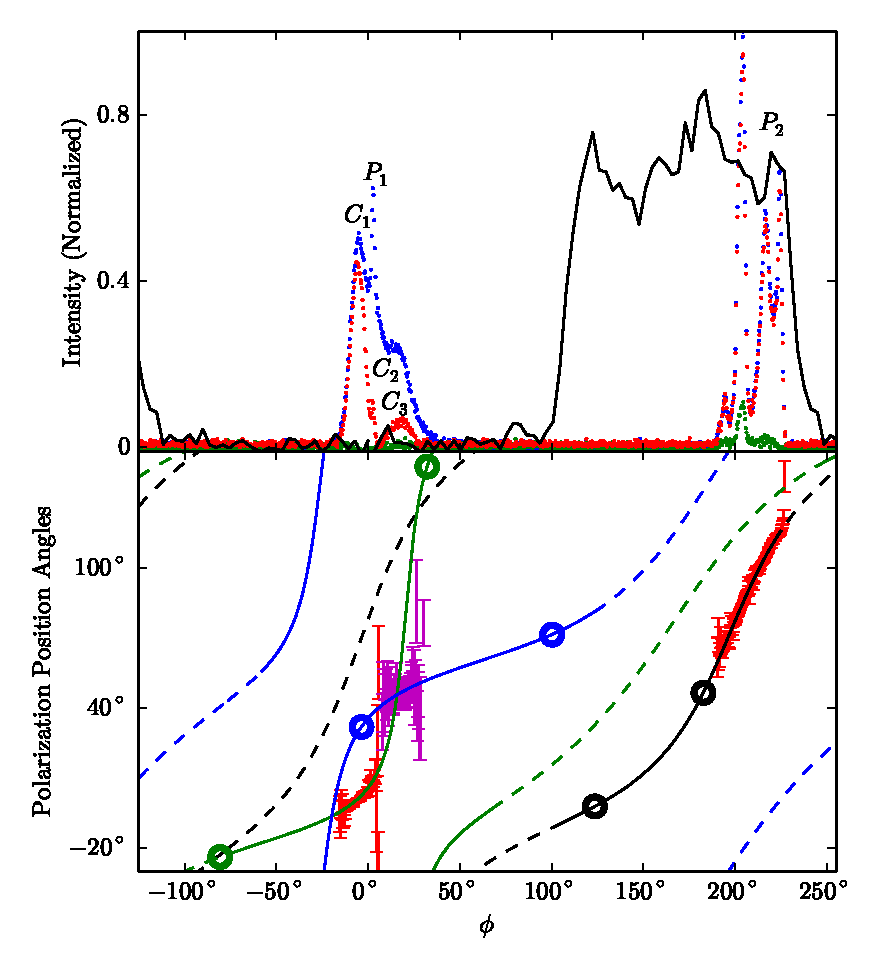
\includegraphics[scale=.8]{chapters/inwardDirectedPhotons/figures/intAndPAJ1057alpha77zeta50V2.eps}
\caption[ Intensity and polarization data for PSR J1057$-$5226 overlaid with bidirectional model]{\label{fig:singleAlt}
In the upper panel, blue points are total radio intensity 
data for 1.5GHz, red points are linear polarization intensity data
and green points are circular polarization intensity data for 
PSR J1057$-$5226.  Black solid line is $\gamma$-ray light
curve for emission greater than 0.1 GeV.
In the bottom panel, red data points with error bars are polarization position angles
in the outward-directed photon emission component (and RVM fit). The magenta data points with error bars are polarization 
position angles included in the inward-directed photon emission component, $P_{2}$.
The model polarization comes from
a fit with (unreduced) $\chi^2=419$ and parameters $\alpha=77^{\circ}$, $\zeta=48^{\circ}$,
and $R_{C_1/C_2}=R_{C_3}=R_{P_2}=0.35R_{\rm{LC}}$.  
The green and black lines are the model polarization for
outward-directed photon emission but from opposite poles.  
The blue line is the model
polarization of an inward-directed photon emission component
from the same pole as the black line. 
Empty circles mark limiting phase of emission from
open field lines with $\rho_{\rm{ypt}}=1R_{\rm{LC}}$.
Solid lines mark allowed emission phase for an effective open zone with
$\rho_{\rm{ypt}}=0.45R_{\rm{LC}}$ which is required for the model 
phase to cover all of the emission phase in the data.
Phase of zero is the point
of closest encounter to the magnetic axis in the model.
}
\end{center}
\vskip -.6truecm
\end{figure*}


\begin{figure}[htbp]
\begin{center}
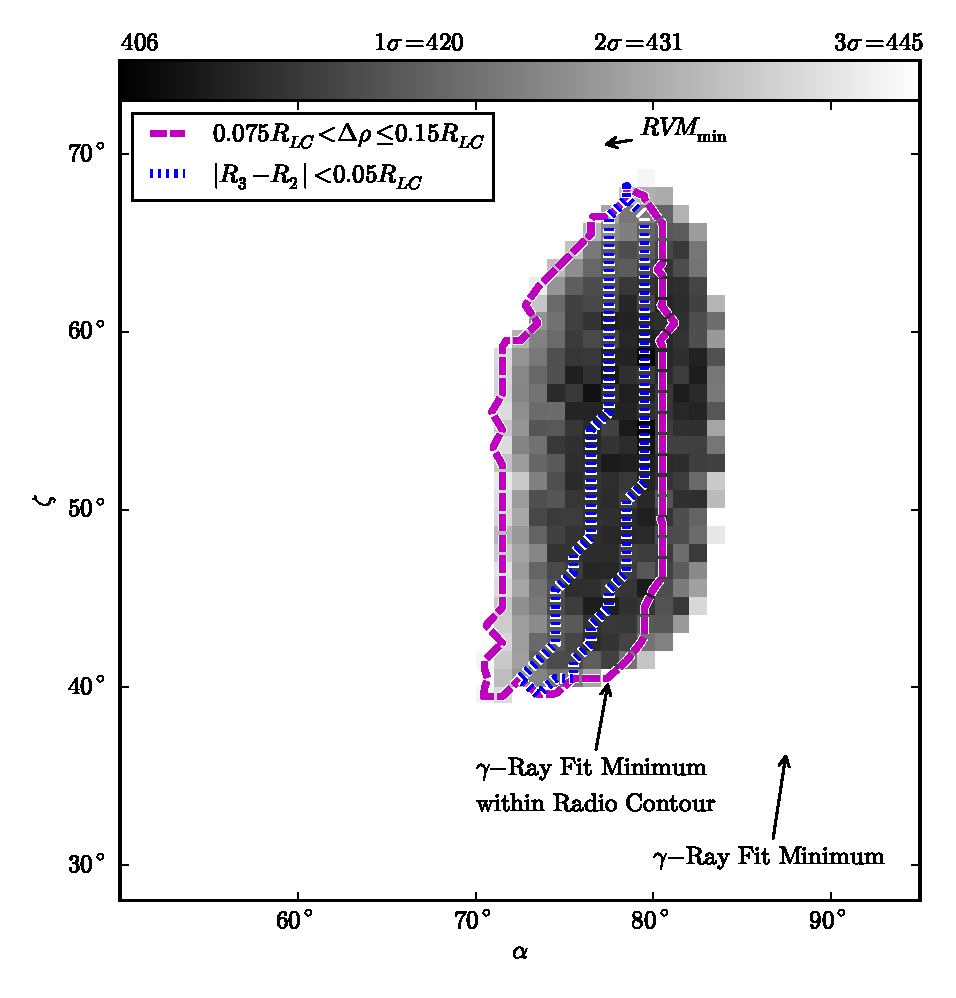
\includegraphics[scale=1]{chapters/inwardDirectedPhotons/figures/J1057-5226Map.eps}
\caption[Map of (unreduced) $\chi^2$ in the $\alpha$-$\zeta$ plane
for a three-altitude bidirectional fit to the polarization data of PSR J1057$-$5226]{\label{fig:map3}
Map of (unreduced) $\chi^2$ in the $\alpha$-$\zeta$ plane
for a three-altitude fit to the polarization data of PSR J1057$-$5226.
Blue contour shows the $3\sigma$ region above $\chi^2_{\rm{min}}$
for emission from the same pole (one outward-directed and one inward-directed)
with similar altitudes ($R_{C_3}$ and $R_{P_2}$).  The magenta contour shows 
the $3\sigma$ region above $\chi^2_{\rm{min}}$ for largest $\Delta \rho$ 
(the cylindrical distance from the largest emission distance to $\rho_{\rm{ypt}}$).
}
\end{center}
\vskip -.3truecm
\end{figure}


\begin{figure}[htbp]
\begin{center}
\includegraphics[scale=1]{chapters/inwardDirectedPhotons/figures/J1057-5226Map323.eps}
\caption[Map of (unreduced) $\chi^2$ in the $\alpha$-$\zeta$ plane
for a three-altitude fit to the polarization data of PSR J1057$-$5226]{\label{fig:c2}
Contours of $3\sigma$ region above $\chi^2_{\rm{min}}$ for three different fits
to the polarization data for PSR J1057$-$5226 in the $\alpha$-$\zeta$
plane. Cyan contour is the $3\sigma$ contour for fitting
the two outward-directed photon emission components (red data points with error bars only,
as seen in Figure~\ref{fig:totDirFitPhi}) with a single altitude ($R_{C_1/C_2}=R_{P_2}$).
The blue contour is the $3\sigma$ contour for the fit with both the two outward-directed
photon emission components and the one inward-directed photon emission component
with a single altitude for $C_1/C_2$ components and another for 
the $C_3$ and $P_2$ components as labeled on Figure~\ref{fig:totDirFitPhi} 
($R_{C_3}=R_{P_2}$).  The red contour is the $3\sigma$ contour
for a single-altitude fit such that $R_{C_1/C_2}=R_{C_3}=R_{P_2}$ with 
inward-directed photon emission for 
component $C_3$.  By assuming
a single altitude, allowed parameter space is strongly constrained.
Even with a two-altitude fit, $\alpha$ is strongly constrained.
}
\end{center}
\vskip -.3truecm
\end{figure}


\begin{table*}[t!!]
\caption{Fit parameters for PSR J1057$-$5226 (Bidirectional Emission)}
\tabcolsep=0.05cm
\begin{center}
\def\arraystretch{2}
\scalebox{0.83}{
\begin{tabular}{lccccccc}
\hline
\hline
& DOF&(unreduced) $\chi^2_{\rm{min}}$ & $\alpha$ ($^\circ$) & $\zeta$ ($^\circ$) & $R_{C_1/C_2}$ ($R_{\rm{LC}}$)& $R_{C_3}$ ($R_{\rm{LC}}$)&  $R_{P_2}$ ($R_{\rm{LC}}$)\\
[.3em] \hline

3 Alt& $228-7$ & $406$ & $76 ^{+7(+7)}_{-3(-6)}$ & $44 ^{+21(+24)}_{-3(-5)}$ & $0.40 ^{+0.06(+0.08)}_{-0.21(-0.28)}$ & $0.47 ^{+0.15(+0.21)}_{-0.36(-0.41)}$ & $0.44^{+0.07(+0.17)}_{-0.35(-0.38)}$  \\ \hline
2 Alt& $228-6$ & $   410 $ & $   77.4 ^{+1.2(1.6)}_{-4.6(-7.4)} $ & $52.4 ^{+12.4(+15)}_{-12.2(-13.8)} $ & $0.34 ^{+0.07(+0.09)}_{-0.14(-0.18)} $ & $0.32 ^{+0.19(+0.25)}_{-0.17(-0.20)} $ &  \\ \hline
1 Alt& $228-5$ & $   419 $ & $   76.6 ^{+0.8(+1.2)}_{-0.6(-1.0)} $ & $47.6 ^{+5.4(+8.2)}_{-3.6(-4.8)} $ & $ 0.35 ^{+0.05(+0.07)}_{-0.02(-0.03)} $ &  & \\ \hline



\end{tabular}}
\tablecomments{ Errors reported without (with) parentheses are for $1\sigma$ ($3\sigma$) from $\chi^2_{\rm{min}}$.}
\label{tb:fit}
\end{center}
\end{table*}





\begin{table*}[t!!]
\caption{Measured Parameters for PSR J1057$-$5226 (Bidirectional Emission)  }
\begin{center}
\begin{tabular}{llll}
\hline
&$\Delta \rho$ ($R_{\rm{LC}}$)& $\rho_{\rm{max}}$ ($R_{\rm{LC}}$)& $\rho_{\rm{ypt}}$ ($R_{\rm{LC}}$)\\
\hline & \\[-1em]\hline

3 Alt&$0.12^{+0.02(+0.02)}_{-0.12(-0.12)}$ & $0.39^{+0.08(+0.16)}_{-0.21(-0.26)}$ & $0.51^{+0.07(+0.14)}_{-0.35(-0.48)}$  \\ \hline
2 Alt&$0.12^{+0.01(+0.02)}_{-0.05(-0.06)}$ & $0.29^{+0.16(+0.22)}_{-0.11(-0.15)}$ & $0.41^{+0.17(+0.23)}_{-0.15(-0.16)}$  \\ \hline
1 Alt&$0.12^{+0.01(+0.01)}_{-0.01(-0.01)}$ & $0.34^{+0.02(+0.03)}_{-0.03(-0.05)}$ & $0.46^{+0.02(+0.03)}_{-0.03(-0.05)}$  \\ \hline

\end{tabular}
\tablecomments{Errors reported without (with) parentheses are for $1\sigma$ ($3\sigma$) from $\chi^2_{\rm{min}}$.}
\label{tb:meas}
\end{center}
\end{table*}

In Figure~\ref{fig:singleAlt}, the best fit single-altitude
model overlays the polarization data of PSR J1057$-$5226. 
Red data points match well to 
outward-directed photon model polarization.  This polarization (outward only)
also matches reasonable well to the RVM model, $\chi^2=325$ (unreduced, Degrees of Freedom $=\rm{DOF}=166-4$).
The best fit RVM model is labeled on Figure~\ref{fig:map3}.
The RVM fit is problematic because it requires emission
from well within the closed zone of the pulsar magnetosphere
\citep{weltevrede2009mapping}.  \cite{craig2014tackling}  fit the red points (in Figure~\ref{fig:singleAlt})
with a finite-altitude model and found even better
fits with altitudes either far from the neutron star or within
the closed zone and fits in between these extremes.  Unfortunately, this model
was unable to model the data points in magenta. 
In the current paper, 
we explored the possibility that 
the magenta points originate from inward-directed photon emission.

Figure~\ref{fig:map3} shows the (unreduced) $\chi^2$ surface in the $\alpha-\zeta$
plane for position angle data modeled using a three-altitude
model with inward-directed photon emission for component $C_3$.  The lowest (unreduced) $\chi^2$
was $406$ with $\rm{DOF}=228-7$.  Table \ref{tb:fit} shows best fit parameters
as well as $1\sigma$ and $3\sigma$ error bars for those parameters.  The blue contour
of Figure~\ref{fig:map3} is the $3\sigma$ from $\chi^2_{\rm{min}}$ contour for models with similar 
$R_{C_3}$ and $R_{P_2}$.  Since component $C_3$ and $P_2$ are from the same pole,
it is not unreasonable to assume they are from similar heights.  The magenta
contour is the $3\sigma$ from $\chi^2_{\rm{min}}$ contour of models with the 
largest $\Delta\rho$ (see Section \ref{sec:fitProcedure} for definitions).  Models with larger $\Delta\rho$ 
are more trustworthy since field lines close to the y-point will be
distorted in manners not accounted for in our vacuum dipole model.  The
component $P_2$ drives this parameter to such small values while components $C_1/C_2$
and $C_3$ for the most part originate well away from the y-point cylindrical distance.
Figure~\ref{fig:singleAlt} illustrates this point well.
Empty circles on the figure mark the expected phase of emission for the 
classical dipole open zone ($\rho_{\rm{ypt}}=1R_{\rm{LC}}$).  For
this particular set of fit parameters $C_1/C_2$ and $C_3$
data are both well within the classical open zone while
$P_2$ data is entirely outside of this phase range.

Figure~\ref{fig:c2} shows the $3\sigma$ from $\chi^2_{\rm{min}}$ contour in the $\alpha-\zeta$
plane of a variety of fitting schemes.  The cyan contour is the $3\sigma$ area 
in the $\alpha-\zeta$ plane of a fit done with only $C_1/C_2$ and $P_2$ data and a single
altitude.  These are the outward-directed photon emission components.  The blue contour represents
the fit with all three components but with different altitudes for the 
different poles ($C_3$ and $P_2$ have the same altitude, similar to the blue
contour on Figure~\ref{fig:map3}).  The fit
represented with the blue and cyan contours both have large ranges
of acceptable $\zeta$.  The red contour is the $3\sigma$ from
$\chi^2_{\rm{min}}$ area for a fit with a single altitude, $R_{C_1/C_2}=R_{C_3}=R_{P_2}$.
Not surprisingly, this is roughly the overlap of the cyan and blue contours.
Further, unlike the blue and cyan contours, the red contour (representing the assumption
of a single altitude) greatly restricts the possible $\zeta$ range.

Table \ref{tb:fit} compares fit parameters assuming one,
two, and three altitudes.  $\chi^2_{\rm{min}}$ did not drastically change
by adding new free parameters (additional altitudes) nor did
the best fit parameters shift drastically.  
Table \ref{tb:meas} shows parameters that can be measured
from the model fitting.  Again these measured parameters remain the
same for different numbers of altitudes although
the allowed range of the parameters decreases with
fewer fit altitudes.

\subsubsection{Fitting PSR J1057$-$5226 with Outward-Directed Photon Emission}
\label{sec:outwardOnly}
We will briefly discuss fit results of simulations with 
only outward-directed photon emission.  We 
fit with a three-altitude model assuming that
the emission for $C_1/C_2$, $C_3$, and $P_2$
all originated from photons directed away from the
neutron star center.
The lowest (unreduced) $\chi^2_{\rm{min}}=435$ ($\rm{DOF}=228-7$).
For this fit, $\alpha=79^\circ$, $\zeta=35^\circ$, $R_{C_1/C_2}=.54R_{\rm{LC}}$, $R_{C_3}=.86R_{\rm{LC}}$,
and $R_{P_2}=.5R_{\rm{LC}}$.  The $\chi^2_{\rm{min}}$ is just inside
the $3\sigma$ contours of the three-altitude fit assuming
an inward-directed photon emission component; the $\chi^2$
increases significantly within a couple of degrees of this $\chi^2_{\rm{min}}$
at $\alpha=79^\circ$, $\zeta=35^\circ$.
Statistically, the bidirectional model is
better suited to the data over a larger region of 
parameter space and it is visually more satisfying.

\subsubsection{Visualizing the Pulsar Configuration}
\label{sec:config}


Figure~\ref{fig:totDirFitPhi} shows one possible configuration
of the pulsar with inward-directed photon emission for component $C_3$
and that produces position angle polarization sweeps similar
to the data (see Section \ref{sec:fitProcedure} for more
details on the fitting procedure).  This particular configuration
produces the best fit $\chi^2$ assuming emission
from a single altitude ($R_{C_1/C_2}=R_{C_3}=R_{P_2}$).

In the figure, the yellow field lines are 
last closed field lines with $\rho_{\rm{ypt}}=1R_{\rm{LC}}$,
and the cyan field lines are those with $\rho_{\rm{ypt}}=0.45R_{\rm{LC}}$.
For all emission from the $P_2$ component to originate
from open field lines, $\rho_{\rm{ypt}}=0.45R_{\rm{LC}}$.  The grey areas in 
Figure~\ref{fig:totDirFitPhi} are the open field line 
caps at an altitude of $0.35R_{\rm{LC}}$ and $\rho_{\rm{ypt}}=0.45R_{\rm{LC}}$.
The black lines on the caps are the boundary of the caps if 
$\rho_{\rm{ypt}}=1R_{\rm{LC}}$.  Note that the yellow field lines
touch the black line boundary while the 
cyan field lines touch the grey cap boundary.

The red curves on the caps indicate the 
emission locations visible at $\zeta=48^\circ$.  Thicker (curved)
red lines indicate regions of signal in the data for this
given configuration (see Figure~\ref{fig:singleAlt}). 
The thick (curved) red line for $P_2$ goes to the
edge of the grey cap; as discussed earlier, $P_2$
is the component that controls $\rho_{\rm{ypt}}$.
The large phase of emission
requires a low $\rho_{\rm{ypt}}$ or a high altitude
to accommodate the 
$P_2$ emission.  In previous fitting that included only 
polarization data from $C_1/C_2$ and $P_2$, we
could find a few solutions with $\rho_{\rm{ypt}}=1R_{\rm{LC}}$
(the classical dipole open cone of emission) 
within the $3\sigma$ contour from $\chi^2_{\rm{min}}$;
but with the addition of fitting $C_3$ data,
these fits are no longer probable.  

Green arrows from the curves indicate the direction of emission.
The arrow from $C_3$ emission goes into the pulsar magnetosphere.
Locations of $C_3$ and $P_2$ emission are on opposite sides of the same pole.
This is necessary geometrically in order for the inward-directed and
outward-directed photon emission to be visible from the same $\zeta$.

\subsection{Combining $\gamma$-Ray Fitting with Radio Polarization Model}
\label{sec:gam}
One striking feature of the PSR J$1057-5226$ $\gamma$-ray data is the overlap in phase
with the radio data.  
The upper panel of Figure~\ref{fig:singleAlt} shows
the $\gamma$-ray light curve in black over the radio emission.  The 
$\gamma$-ray light curve lines up with the $P_2$ pulse suggesting that
both could be coming from similar locations in the magnetosphere.  
This is an unusual feature for pulsar emission and may give evidence to 
the seemingly unusual emission from the $P_2$ component.

\subsubsection{$\gamma$-Ray Model Method}
%gamma and radio come from same place

The $\gamma$-ray
data was obtained from the \textit{Fermi} LAT pulsar catalog (\citealp{abdo2010fermi,abdo2013second}).
The data is from energies greater than $0.1$ GeV.
The $\gamma$-ray model is based on \cite{romani2010constraining}.  
The outer gap model
has emission originating from inside the effective light cylinder ($\rho_{\rm{ypt}}$)
and beyond the null charge surface ($\vec{B}\cdot\vec{\Omega}=0$).  We use the same emissivity function 
($e^{-[(s-2 s_{\rm{NC,min}}-1)/0.1]^2}$ for beyond a path length of $1+2 s_{\rm{NC,min}}$ and constant below, where 
$s$ is the path length, $s_{\rm{NC,min}}$ is the minimum path length of field lines at a given fraction of the polar cap, and
units are in terms of $R_{\rm{LC}}$) as \cite{romani2010constraining}.
Emission was allowed for a range of effective $w$ values
from $.01$ to $.12$ where $w$ is the fraction of the radial distance
from the pole on the polar cap.  Here we use an ``effective''
$w$ in that the polar cap defined by the open field lines will shift
based on $\rho_{\rm{ypt}}$.  A Gaussian width was applied to a given $w$ 
slice of $0.02$ (again similar to \citealp{romani2010constraining}).

\subsubsection{$\gamma$-Ray Model Results}

\begin{figure}[t!!]
\begin{center}
\includegraphics[scale=.7]{chapters/inwardDirectedPhotons/figures/plotBestFits.ps}
\caption[Data and best models for $\gamma$-ray light curve of PSR J1057$-$5226]{\label{fig:gammaBestFits}
Black data points with error bars are $\gamma$-ray data for energy greater than $0.1$ GeV.
The magenta line is the best fit $\gamma$-ray light curve using extrapolated 
parameters.  The green line is the best fit $\gamma$-ray light curve using
parameters only within the $3\sigma$ from $\chi^2_{\rm{min}}$
space of the radio fit results.  The cyan line is the
best fit $\gamma$-ray light curve using the parameters at the 
best radio fit for a single-altitude model.}
\end{center}
\vskip -.4truecm
\end{figure}


\begin{figure}[t!!]
\begin{center}
\includegraphics[scale=.7]{chapters/inwardDirectedPhotons/figures/plotCombinedw60w150.ps}
\caption[Data and variable $w$ model for $\gamma$-ray light curve of PSR J1057$-$5226]{\label{fig:gammaCombinedw60w150}
Black data points with error bars are $\gamma$-ray data for energy greater than $0.1$ GeV.
The blue line and red line are $\gamma$-ray light curves using the parameters at the 
best radio fit for a single-altitude model and $w=0.15$ and $w=0.06$.
The magenta line is a $\gamma$-ray light curve from a model that illuminates 
field lines between $w=0.15$ and $w=0.06$ from one end of the light curve to the other.
This model illustrates that better model light curves are possible in regions of 
the best fit radio models but they would require modifications to 
the prescription of illuminated field lines.
}
\end{center}
\vskip -.4truecm
\end{figure}



We limited our parameter space to $\alpha$, $\zeta$, $\Delta \phi$, and
$\rho_{\rm{ypt}}$ within $3\sigma$ of the $\chi^2_{\rm{min}}$
of the radio modeling results.  Additionally,
$\rho_{\rm{ypt}}$ obtained in the radio polarization fitting is
an \textit{upper} limit and the lower limit is set by 
the geometrical location of the radio emission
with the largest cylindrical distance from the spin axis.
We focused on fitting with only maximum $\rho_{\rm{ypt}}$ since smaller
y-point distances revert the model to essentially a simple
dipole.  This in turn eliminates the caustics and box-like
sides of the emission which are clearly seen in the data 
(see Figures~\ref{fig:gammaBestFits} and \ref{fig:gammaCombinedw60w150} for data).
In general, models with smaller $\rho_{\rm{ypt}}$ yield
worse fits because of this.  Further, fits with  larger
$\zeta$ ($\gtrsim 55^\circ$) tended to have smaller
required $\rho_{\rm{ypt}}$ (from radio fits) and 
poorer $\chi^2$ values due to this.

With this relatively simple $\gamma$-ray model
and the radio fit restrictions, the best fit model is
$\alpha=77^\circ$, $\zeta=40^\circ$, $w=0.04$, with unreduced $\chi^2_{\rm{min}}=695$.
The degrees of freedom for the $\gamma$-ray fits are $\rm{DOF}=100-1$ since
only $w$ is being fit.
Here the $\chi^2_{\rm{min}}$ in radio is 445 right at the $3\sigma$
cut off of the fits.  



Admittedly, the $\gamma$-ray model is not
exact, neglecting important plasma physics that can
affect the field line structure, particularly at
high altitudes, in addition to making simplistic 
assumptions about $\gamma$-ray production locations.  Further, having the minimum 
$\chi^2$ region for the $\gamma$-ray model close to the minimum
in polarization is encouraging even if they do not
exactly overlap and still indicates some real features are
being captured by the model.
Since the minimum $\chi^2$ of the $\gamma$-ray model is right at the 
3$\sigma$ edge of the $\chi^2$ surface of the radio polarization fit, we are interested in
the behavior of the $\gamma$-ray model beyond this region.
Calculating $\chi^2$ values of the $\gamma$-ray model
using radio fit model values is not sensible since radio models beyond $3\sigma$
do not contain real information and are poor matches to the data.
Instead, we expanded the allowed region
around this fit space for the radio model within $3\sigma$ 
of $\chi^2_{\rm{min}}$by extrapolating parameters using simple piece-wise
linear fitting. 

The lowest local unreduced $\chi^2$
is 322 with $\alpha=87^\circ$, $\zeta=36^\circ$, $w=0.02$ 
for fits in the extrapolated region.
Decreasing $\zeta$ further resulted in the worsening of $\chi^2$.
Unfortunately the unreduced $\chi^2$ for the radio is 3400, far beyond what 
would be statistically acceptable and visually unsatisfactory.  

On Figure~\ref{fig:map3} is a marking for the lowest $\chi^2$ from the $\gamma$-ray 
fitting both within the $3\sigma$ radio fit contour and 
without the contour. Ideally, the best fit $\gamma$-ray model would fall
within the best fit parameter space of the polarization radio model.
But considering the uncertainties of the $\gamma$-ray model,
the lowest local $\gamma$-ray $\chi^2$ is not
dramatically far from $\chi^2$ minimum area of the 
radio polarization fit.   
From this information we can conclude that a joint
fit between radio and $\gamma$-ray data would fall around $\zeta\sim40^\circ$.

Figure~\ref{fig:gammaBestFits} shows the best fit light curves
for within the $3\sigma$ contour of the radio results (green)
and the local minimum fit in the $\gamma$-ray just 
beyond this contour (magenta).  Both appear relatively 
flat compared to the data.  Also plotted in the same figure 
in cyan is the best fit light curve at $\alpha=77^\circ$, $\zeta=48^\circ$ 
(unreduced $\chi^2=5000$, $\rm{DOF}=100-1$),
the best fit values in the radio polarization for the single-altitude model. The model light curves are normalized to the total 
counts.

The \textit{position} of the pulse
using this $\gamma$-ray model 
matches the light curve position; the morphology of the 
peaks within the pulse are not matched. 
If $w$ is not constant, models much more suited for the single-altitude
polarization fit space in terms of pulse width are obtainable.  
Whether this would improve the morphology is unclear but 
certainly possible.
At the moment, a prescription
for a $w$ that is variable is unclear.

To illustrate this point, we produced a 
light curve which varied between $w=0.06$ and $w=0.15$
(linearly with respect to magnetic $\phi$).  This
light curve is plotted in Figure~\ref{fig:gammaCombinedw60w150}
over the data.  
The curve is not fit to the data but is meant simply 
as an illustration; undoubtedly, using a different prescription
for field line illumination or slightly different $\alpha$ and $\zeta$
could result in better fits to the data in the $3\sigma$ parameters
space of the radio data.  But without a
clear and physically motivated prescription, any curves would be 
purely ungrounded speculation.
Also plotted in Figure~\ref{fig:gammaCombinedw60w150}
are light curves with constant $w=0.06$ (solid, red) and $w=0.15$ (dashed, blue).

We can therefore conclude that the $\gamma$-ray 
fitting favors smaller $\zeta$ but perhaps not quite
as strongly as may be suggested by models where field lines
of a single $w$ are illuminated.  Either way, results suggest a lower $\zeta$
than that of RVM ($\alpha=77^\circ$, $\zeta=70^\circ$, ignoring the $C_3$ component) 
which is consistent with bidirectional, finite-altitude radio polarization fitting. 

\subsection{Discussion and Conclusions}
\label{sec:conclusions}

\subsubsection{Comparison to \cite{weltevrede2007main}}

The bidirectional model of PSR J1057$-$5226 presented in \cite{weltevrede2007main} 
(Figure 12) is different from the one presented in
the current paper.  The configuration for PSR J1057$-$5226 is very similar to
the one given for PSR B1702$-$19 in the same paper.  Our particular
configuration was motivated by the shape of the polarization curve while
the configuration of \cite{weltevrede2007main} was motivated by modulations
in the intensity.  First, the model of \cite{weltevrede2007main} Figure 12
divides the emission of the pulse $P_2$ into a modulated and an
unmodulated component.  The paper \cite{weltevrede2012phase} does support
$P_2$ having several different modulations among the peaks.  Yet the
polarization of $P_2$ is smooth and connected between the various
components and thus the emission is very likely to come from the same
location in the magnetosphere.  Second, the model of \cite{weltevrede2007main} 
has the emission from the pulse we label as $P_1$ from a single
location in the magnetosphere whereas in the model presented here
the $P_1$ pulse is split into outward-directed photon emission and
inward-directed photon emission.  The motivation here was again driven
by the polarization sweep.  A clear disconnect exists between the
polarization of components $C_1/C_2$ and the component $C_3$.  Considering these two pieces of
polarization are from the same pole, whether the emission was from
outward-directed photons (as discussed in Section \ref{sec:outwardOnly}) or from
inward-directed photons (with and without multiple altitudes and
orthogonal mode jumps), did not yield appropriate models.  The best fit
model with the pulse $P_1$ emitted wholly from inward-directed photons and
$P_2$ emitted from outward-directed photons had an unreduced $\chi^2$ of $786$.  

On the other hand, the polarization of $C_1/C_2$ and $P_2$ are well-defined with
small error bars while the polarization of $C_3$ has
larger error bars and is generally more noisy.  It is
then natural to assume that the emission of $C_1/C_2$ and $P_2$ is typical,
outward-directed photon emission and the emission of $C_3$ is unusual.
Further, the emission of component $C_3$ is located after the phase of
emission of components $C_1/C_2$, the location where emission from
inward-directed photons of the opposite pole would appear.  Thus the
model configuration used in this paper was a natural choice before any
formal fitting was performed.


\subsubsection{Comparison to \cite{weltevrede2009mapping}}

As noted earlier, \cite{weltevrede2009mapping} analyzed polarization data of
PSR J1057$-$5226.  They use the RVM to calculate polarization sweeps.
The magnetic field lines are simple vacuum dipole (RVM) but they included
retardation and aberration effects to calculate the height estimations
from BCW. In addition, they use pulse width arguments to calculate emission 
height.  They estimate the
altitude of emission from both poles  is $0.07R_{\rm{LC}}$.  At this altitude, the
polarization sweeps will not be drastically distorted \citep{craig2012altitude} 
and RVM is appropriate to use assuming this altitude.  Also at this altitude, the
magnetic field lines in the numerical model will be essentially the same
as RVM.  Further, at low altitudes, polarization position angles for
inward-directed photons and outward-directed photons will be similar.
The polarization of VII as labeled in \cite{weltevrede2009mapping}
(corresponding to $C_3$ in the current paper) is unlikely to have strongly
influenced the RVM polarization fitting since there are few data points
for $C_3$ and these data points have larger error bars compared to the rest
of the polarization sweep (as can be noted from Figure 2 of \citealp{weltevrede2009mapping}).  
With these considerations and if the numerical model used
in the current paper were applied to the data of \cite{weltevrede2009mapping}
with a low altitude constraint, the polar cap map of Figure 7 in
\cite{weltevrede2009mapping} would be similar.  The difference would be that
the VII line section (the inward-directed photon emission) would be
located in the upper left quadrant and on the same pole as the
I-II-III-IV line section of the diagram.

In \cite{weltevrede2009mapping}, they describe the last closed field lines
needed for the emission to originate from open field lines in terms of a
footprint parameter.  This footprint parameter is a measure of the cap
size on the neutron star surface.   In addition, for their favored
configuration, they state that the last closed field line closes at a distance
of a quarter of a light cylinder radius (e.g. $\rho_{\rm{ypt}}=0.25R_{\rm{LC}}$).  For our best
fit single-altitude models $\rho_{\rm{ypt}}\sim0.46R_{\rm{LC}}$ and $R\sim0.35R_{\rm{LC}}$.  The favored
altitude of  \cite{weltevrede2009mapping} is $0.07R_{\rm{LC}}$.  Roughly, the model
presented here is a natural extension of the \cite{weltevrede2009mapping}
model that allows larger finite altitude.  Because our model allows
larger altitudes, the needed $\rho_{\rm{ypt}}$ is consistently higher.  Our $\Delta \rho_{\rm{ypt}}$
(the cylindrical distance between the maximum emission distance and the
effective light cylinder) is $\sim0.12R_{\rm{LC}}$.  For \cite{weltevrede2009mapping}, we
can estimate $\Delta \rho_{\rm{ypt}}$ as $0.25-0.07=0.18R_{\rm{LC}}$ which again is roughly
consistent with the numerical model.

\subsubsection{Comparison to \cite{weltevrede2012phase}}
\label{sec:comp2012}
In \cite{weltevrede2007main}, the authors argued for a bidirectional model
for PSR B1702$-$19 based on phase locked modulation and include a schematic 
of a possible PSR J1057$-$5226
bidirectional model.  However, in \cite{weltevrede2012phase}, bidirectional
emission models are avoided presumably because 
the phase locked modulation delay is too large
for the simple time of flight delay for bidirectional emission
from the same location in the magnetosphere.  The
model relies on emission from the exact same location in the
magnetosphere for both
inward-directed and outward-directed photons.  
For our model, the emission is from the same pole but on
opposite sides of the pole.  Thus a
larger difference in modulation delay time
may not be reasonable.

Further, the modulation reported in \cite{weltevrede2012phase} are present
mostly in the peaks we label as $C_1$ and $C_2$.  These peaks (labeled as V
and VI in \citealp{weltevrede2012phase}) are modeled as forward-directed photon
emission.  The trailing edge of the pulse (mostly the peak labeled as $C_3$
in the current paper and VII in \citealp{weltevrede2012phase}) does not
participate in the $2.5P$ modulation.  If the phase-locked modulation was
connected to the bidirectional emission model presented here, the peak
$C_3$ (modeled as originating from the inward-directed photons) should
modulate with the $P_2$ peak.

Finally, the modulation in $C_1$ and $C_2$ and the lack of modulation in $C_3$
indicates that $C_1$ and $C_2$ are distinct from $C_3$.  This supports the
bidirectional model since $C_1$ and $C_2$ come from the opposite pole compared
to $C_3$.  In this model we would not expect emission from these different
peaks to modulate with one another.


\subsubsection{Summary}
The position angle polarization data for PSR J1057$-$5226 is inconsistent with
the typical geometrically-based polarization model, RVM.  Based
on the data, RVM was modified to include orthogonal mode
jumps, multiple finite altitude, and bidirectional emission.
With these modifications, the produced
polarization position angle sweeps are consistent with the data.  
Assuming a single altitude of emission greatly
restricts the acceptable parameter space. 
The data still requires the
y-point further in than the classical
light cylinder distance but this atypical behavior may 
lend hints to the bidirectional nature of PSR J1057$-$5226.


Further, $\gamma$-ray modeling with a model of the simplest outer gap
formulation is possible.  The $\gamma$-ray models favor the smallest $\zeta$
values when restricted 
by radio model fitting parameters within
$3\sigma$ of $\chi^2_{\rm{min}}$.
These models do capture the overall shape of the pulse but a more precise fit
will likely required better understanding of the location of the $\gamma$-ray
emission.   Additionally, in our current model, we neglect plasma effects which
might be important at the altitudes that are modeled here.  Further,
PSR J1057$-$5226 has unusual modulation patterns in its intensity.  Surely, these
modulation hold tantalizing keys to the pulsar emission and indicate
atypical behavior; yet we are unable to incorporate these modulations in our
model.


In brief, bidirectional emission is consistent with both
radio and $\gamma$-ray data and is an
exciting possibility for the unusual emission
of the pulsar PSR J1057$-$5226.


\acknowledgements
We greatly thank S. Johnston for supplying radio data for PSR J1057$-$5226 (2012, private correspondence)
and Roger W. Romani for valuable discussion. This work has been 
supported by the Stanford Office of
the Vice Provost of Graduate Education DARE Doctoral
Fellowship Program to H.A.C.



\section{Exploring Inward-Directed Photon Emission Using Radio Polarization Data of PSR J1705$-$1906}
\paperref{This section is based on work done for private corresponds in relation to
``Six Faint $\gamma$-Ray Pulsars Seen with the {\it Fermi} Large Area Telescope. 
Towards a Sample Blending into the Background'' 
\citep{hou2014six}.}

In the previous section, we discussed extensively the application
of a bidirectional model to the data of PSR J1057$-$5226.
We additionally applied the bidirectional model to the
polarization position angle data of PSR J1705$-$1906
and will discuss the results in this section along with
giving an overview of past studies of this pulsar.
Overall, the results of the analysis of 
PSR J1705$-$1906 are not as compelling or 
conclusive as those of PSR J1057$-$5226 but
are nevertheless reported here for completion.

\subsection{Past Studies}
The pulsar PSR J1705$-$1906 (PSR B1702$-$19) has been identified by \cite{weltevrede2007main}
as a possible candidate for bidirectional emission.
The second component of the main pulse (as labeled by \cite{weltevrede2007main} 
and the pulse with the highest intensity) and the interpulse 
have a phase locked delay.  The main pulse modulation lags that of the
interpulse by $0.43$ rotation period, around the $0.5$ rotation period expected from a geometric delay.
These modulations occur approximately every $10.4$ rotation periods.

\cite{weltevrede2007main} explored evidence of two-pole emission in the
polarization data.  As  \cite{weltevrede2007main} 
noted, a U-shape in the interpulse polarization
data is difficult to model and they fit the polarization
data to the rotating vector model (RVM) both including and excluding
this difficult section.
They further restrict their fits using beaming radius and
width of emission phase arguments.  They also
discuss a single wide cone model.  For the RVM, 
emission from a single wide cone, from both poles, and from a single
pole with bidirectional photons will
have the same polarization sweep due to the lack of relativistic and sweep-back effects.
In order to create a single wide cone model they restrict
$\phi$ (the location in phase of model phase zero) to 
vary between $125^\circ$ and $215^\circ$.  
Fits with these constraints yield $\chi^2$ far worse
than those of a two pole model.

Further, \cite{weltevrede2007main}
examined the inner and outer cone model of \cite{gil1985interpulse}.
With radius beam arguments, they estimate
the difference in emission height between the two
emission regions for this model to be $900$ km
($0.064R_{\rm{LC}}$) which should correspond to a difference in 
phase of $7^\circ$ (see Section \ref{sec:beamingGeometry}
for beaming model details).  Any difference in phase between the 
interpulse and main pulse is much smaller and they therefore
ruled out this model.

Finally for bidirectional  
emission, we would again expect a delay in phase
for any configuration other than the simplest configuration.
This is not seen in the data.  The difference between
the centroid of the interpulse and the minimum between 
the two main pulse components is nearly $180^\circ$.
Alternatively, the phase difference between the two {\it modulating}
components is $176^{\circ}$.  Again using radius beam arguments
and time delay arguments, \cite{weltevrede2007main} gave 
emission height estimates.


\subsection{Polarization Analysis}

\begin{figure}[t!!]
\begin{center}
\includegraphics[width=0.98\textwidth]{chapters/inwardDirectedPhotons/figures/mapB1702allForward.eps}
\caption[The $\chi^2$ map in the $\alpha$-$\zeta$ plane
for fitting polarization sweep data from PSR J1705$-$1906
to a model with only outward-directed photon emission
from two poles]{
The $\chi^2$ map in the $\alpha$-$\zeta$ plane 
for fitting polarization sweep data from PSR J1705$-$1906
to a model with only outward-directed photon emission
from two poles.  
The data fits reasonable well on a wide variety of 
$\alpha$ and $\zeta$ although large $\alpha$ and $\zeta$
are favored.  Red contours are those fits within
$3\sigma$ of the $\chi^2_{\rm{min}}$
with smaller altitudes of emission and
cyan contours are those fits within
$3\sigma$ of the $\chi^2_{\rm{min}}$ with larger 
altitudes of emission.
Black contours are those fits within
$3\sigma$ of the $\chi^2_{\rm{min}}$
and assume only the classical 
open field line emission.
Green contours, on the other hand, allow for
$\rho_{\rm{ypt}}$ as low as $0.5R_{\rm{LC}}$.
\label{fig:allForward}
}
\end{center}
\end{figure}

\begin{figure}[t!!]
\begin{center}
\includegraphics[width=0.98\textwidth]{chapters/inwardDirectedPhotons/figures/mapB1702SinglePole.eps}
\caption[The $\chi^2$ map in the $\alpha$-$\zeta$ plane
for fitting polarization sweep data from PSR J1705$-$1906
to a model with only outward-directed photon emission
from a single pole]{
The $\chi^2$ map in the $\alpha$-$\zeta$ plane
for fitting polarization sweep data from PSR J1705$-$1906
to a model with only outward-directed photon emission
from a single pole.
The data fits reasonable well on a wide variety of
$\alpha$ and $\zeta$ although large $\alpha$ and $\zeta$
are favored.  The region is also more
constrained compared to the two-pole fit.
Red contours are those fits within
$3\sigma$ of the $\chi^2_{\rm{min}}$
with smaller altitudes of emission and
cyan contours are those fits within
$3\sigma$ of the $\chi^2_{\rm{min}}$ with larger
altitudes of emission.
Black contours are those fits within
$3\sigma$ of the $\chi^2_{\rm{min}}$
and assume only the classical
open field line emission.
Green contours, on the other hand, allow for
$\rho_{\rm{ypt}}$ as low as $0.5R_{\rm{LC}}$.
\label{fig:singlePole}
}
\end{center}
\end{figure}

\begin{figure}[t!!]
\begin{center}
\includegraphics[width=0.98\textwidth]{chapters/inwardDirectedPhotons/figures/mapB1702IPBackward.eps}
\caption[The $\chi^2$ map in the $\alpha$-$\zeta$ plane
for fitting polarization sweep data from PSR J1705$-$1906
to a model with bidirectional photons from a single pole]{
The $\chi^2$ map in the $\alpha$-$\zeta$ plane
for fitting polarization sweep data from PSR J1705$-$1906
to a model with bidirectional photons from a single pole.
Again, the data fits reasonable well on a wide variety of
$\alpha$ and $\zeta$. Large $\alpha$ and $\zeta$
are favored although not as large as those for the 
previous two fitting schemes (all outward-directed emission
and single pole emission).  Red contours are those fits within
$3\sigma$ of the $\chi^2_{\rm{min}}$
with smaller altitudes of emission and
cyan contours are those fits within
$3\sigma$ of the $\chi^2_{\rm{min}}$ with larger
altitudes of emission.
Black contours are those fits within
$3\sigma$ of the $\chi^2_{\rm{min}}$
and assume only the classical
open field line emission.
Green contours, on the other hand, allow for
$\rho_{\rm{ypt}}$ as low as $0.5R_{\rm{LC}}$.
\label{fig:inward}
}
\end{center}
\end{figure}

Here we present our own analysis of the 1.408 GHz polarization 
data \citep{gould1998multifrequency} using the multiple-altitude model
with bidirectional photon emission.
Similar to \cite{weltevrede2007main}, three scenarios are
examined: emission from two poles emitting only forward-directed
photons, emission from a single wide pole emitting only forward-directed
photons, and emission from a single pole with bidirectional photons (both inward-
and outward-directed).  For the latter case, the peak identified as the interpulse
is assumed to originate from inward-directed photons.

Figure~\ref{fig:allForward}
shows fit results for pulsar PSR J1705$-$1906 
for the typical configuration with emission from
two separate poles for the two different pulses.
Figure~\ref{fig:singlePole}
shows fit results for a configuration where
emission originates from a single wide pole.
Figure~\ref{fig:inward}
shows fit results for a configuration where 
polarization of the ``main pulse'' as identified by \cite{weltevrede2007main}
originates from outward-directed photons and 
``interpulse'' polarization originates from the same pole 
but from inward-directed photons.
Also shown on the graphs are contours for high and low altitude cuts,
classical open zone constraints ($\rho_{\rm{ypt}}=1R_{\rm{LC}}$),
and restricted y-point lowering constraints in which emission is allowed from
the closed zone.
Overall, the results are not very constraining.
All three fits have $\chi^2_{\rm{min}}\sim60$ for DOF$=22-5$.
Also note that only a single altitude was applied for all components of the
polarization sweep.  Allowing for multiple altitudes would make the
fitting even less constraining.
The long, thin contour along the diagonal of the graphs 
is the RVM fit.  For the RVM fitting, $\chi^2_{\rm{min}}=65$ such
that the use of finite altitudes is not well justified statistically.

Although $\gamma$-ray fitting is not formally performed,
\cite{hou2014six} notes using results from \cite{Watters:2010jb}
some constraints to the fit parameters.
They conclude that $\alpha>50^\circ$ and $\zeta<60^\circ$
although this too is not very constraining.  Overall,
better data is likely needed to make more meaningful
conclusions about PSR J1705$-$1906 and the possibility of
inward-directed photon emission.





\chapter{Outlook and Perspective}
\label{chapter:outlook}

\section{Next Steps}
\label{sec:future}

In this thesis, we brought a fresh perspective 
on the modeling of polarization of pulsars
and questioned the current modeling assumptions.
Although the work presented here 
is an improvement on our understanding
of polarization, the need to go still further
is continuously present.
To understand all the data, the model
needs a fundamental change.  Although we did a fair
job in explaining the polarization presented
here, there is still a wealth of pulsar
polarization data that has not been analyzed
and will likely not be understood with the
model revisions presented here alone.

The data that was available for analysis
was limited.  Often times, only a single frequency 
was available for analysis or the frequency with the
most data or smallest error bars was analyzed.
The frequency maps to the altitude \citep{cordes1978observational} 
such that different frequency originate at different
altitudes.
But this mapping    
was never tested due to inadequate data.
As this is a multi-altitude model, having not applied
this model to multi-frequency data within radio
is a blatant shortcoming of this thesis.
Further, the data was averaged over many periods,
averaging out potentially interesting features.  
For instance the polarization of PSR J1057$-$5336
and PSR J1705$-$1906 have periodic nulling as discussed 
in Chapter \ref{chapter:inwardPhotons} which is related to bidirectional
emission; it is possible that analyzing the polarization
data at different times in this cycle may 
yield further insights.
Arguably, a population study is needed
to fully understand the nature of the polarization
data from pulsars instead of focusing so much on
individual sweeps.

Throughout the analysis,
a single altitude of emission for each component
of the polarization was used. 
The use of a single-altitude model cannot produce the
sharp intensity peaks seen in the radio light curve.
In the $\gamma$-ray emission, these sharp peaks in the intensity 
are called caustic peaks and are caused by 
overlapping of emission from a range of altitudes.
In the outer gap model of $\gamma$-ray emission,
these caustic peaks naturally arise from tracing
emission from a single field line transversing through the 
magnetosphere, away from the pulsar.
In the radio model, a single altitude assumption will not 
result in sharp peaks.  A multiple-altitude model would not
be hard to implement with emission for a single component
originating over many altitudes but the prescription of
such an assumption is unclear, thus we assumed the simplest 
model of just a single altitude.

Scattering effects sometimes appear in the polarization
for pulsars where interstellar scattering is low.
For instance, in the paper \cite{karastergiou2009complex},
the author argues a combination of mode
jumps and interstellar scattering
can produce the complex polarization sweeps seen in 
the pulsar data.
The pulsar polarization sweep that the author uses as the
example to which this model is applicable is the data of
PSR B0355$+$54 (PSR J0358$+$5413).
In reality the scattering time constant for 
this pulsar is small compared to the
amount of scattering needed to 
cause the amount of smoothing seen in
the polarization sweep and particularly
between the supposed mode jumps.
We also saw more scattering in PSR J1420$-$6048
than could be explained by the given scattering
time constant (Section \ref{sec:J1420}).
Although we did not formally report the
fitting results of PSR J1600$-$3050 \citep{yan2011polarization},
in preliminary fitting, increasing the scattering time
constant did improve the $\chi^2$ significantly. But
compared to the time constant needed \citep{cordes2002ne2001} 
such fits were unphysical considering the interstellar scattering.
This could indicate internal scattering in the magnetosphere
\citep{braje2001magnetospheric} although such claims would require further investigation
and another set of revisions to the current model.

Our model is based on the vacuum dipole.  This model
is acceptable at low altitude but in some cases,
high altitude limits in the fitting of the
model to the data were explored.  At high altitudes, plasma effects 
become important and a force-free model would be
more appropriate.  

\cite{spitkovsky2006time} first used a time-dependent
numerical code to calculate non-axisymmetric
magnetic fields of a force-free model.
The plasma filled, force-free models that require magnetohydrodynamic
simulations are used for modeling light curves of
high altitude emission in the $\gamma$-rays
\citep{contopoulos2010pulsar,bai2010modeling}.

The time-dependent Maxwell equations are given as
\begin{equation}
\frac{\partial \vec{B}}{\partial t}=-\vec{\nabla} \times \vec{E} 
\end{equation}
\begin{center}
and
\end{center}
\begin{equation}
\frac{\partial \vec{E}}{\partial t}=-\vec{\nabla} \times \vec{B} - 4\pi \vec{J}. 
\end{equation}
And with the force free assumption, we get
\begin{equation}
\vec{J}=\frac{1}{4\pi B^2} \lbrack (\vec{\nabla}\cdot\vec{E}) \vec{E}\times\vec{B} + (\vec{B}\cdot\vec{\nabla}\times\vec{B}-\vec{E}\cdot\vec{\nabla}\times\vec{E})\vec{B}  \rbrack
.
\end{equation}
In the simulations, the above equations are integrated forward in time
\citep{yee1966numerical}
until a steady state is obtained.

\cite{harding2011gamma} modeled $\gamma$-ray light curves
using both vacuum and force-free simulations and
compared to data.
They found that data actually favored
the vacuum models.
Pulsar $\gamma$-ray emission in these models originate
from outer gaps in the plasma-filled magnetosphere
but this study suggests that field lines resemble more
the vacuum models, hinting that the true
solution needs properties of both.

Recent work by \cite{kalapotharakos2012gamma,kalapotharakos2012toward,kalapotharakos2014gamma}
has explored models that
bridge between vacuum and force-free magnetospheres using a finite
conductivity.  
One way of obtaining such a model is by expressing $\vec{J}$
as 
\begin{equation}
\vec{J}=\frac{\vec{\nabla}\cdot\vec{E}}{4\pi} \frac{\vec{E}\times\vec{B}}{B^2} + \sigma \vec{E_{||}}.
\end{equation}
The conductivity $\sigma$ can be varied from 0 to $\infty$
to range between the two standard magnetosphere approximations.
The focus of these papers was again on $\gamma$-ray light curves.
For instance, \cite{kalapotharakos2012gamma} used this
model to synthesize a population study of $\gamma$-ray
pulsars.
But such a model is appropriate for high-altitude radio emission.
Producing polarization sweeps from such a model is sure to 
bring new insights to the magnetospheric emission far from the neutron star.


\section{Summary of Conclusions}
\label{sec:finalConclusion}

The current state-of-the-art, well-used analysis
tool for understanding pulsar polarization is 
the RVM formulation.  Using the simplest model
for analysis is not intrinsically wrong.  Indeed,
when faced with a choice, the simplest model and assumptions
often are the most likely to quickly and clearly
give insights into a physical problem.
Yet, in this thesis we have shown again and again 
the need for a better model to extract all of the
information from the magnetic field lines of pulsars.
In the end, the simple RVM does not work for
complex polarization and for polarization from emission
high in the magnetosphere.  This polarization contains
helpful information about the magnetic field lines which
in turn tells us about the orientation of the pulsar
and the region of emission.  To extract this information,
model assumptions must be revisited.

The limits of 
the analytical models of pulsar polarization including
RVM and beyond were explored.
Through comparison to numerical models, we conclude
that the typical models are
accurate for low altitude emission but
approximations quickly break down at higher altitudes.

Next, in our analysis of complex polarization sweeps from 
high energy pulsars, we included relativistic and
sweep-back effects \citep{romani2010constraining}, 
interstellar scattering \citep{cronyn1970analysis}, 
and orthogonal mode jumps \citep{backer1976orthogonal}. But more
importantly, finite altitudes and multiple altitudes were used to explain a number
of jumps in the polarization data.
The possibility of bidirectional emission from a couple of 
promising pulsars was explored. Overall, there is evidence of high altitude
emission in the radio from the practical application
of the model to the available data.

This thesis work is significant because there are no widely-accepted
alternatives to simple analytical modeling of pulsar polarization position
angles. The analytical model does not
account for effects of the pulsar rotational motion. The simple analytic models
work well for a large number of the known pulsars but fails for young pulsars
and millisecond pulsars which often have complicated polarization. By making
physically motivated models guided by the data, we have been working to
increase the understanding of pulsars emission mechanism and geometry and to
explain discrepancies between data and previous models.


This thesis has laid the groundwork for future endeavors
in extracting knowledge from pulsar polarization data.  It is not an end in
itself but a step beyond the well-established but insufficient
polarization models. Significant steps are still needed
to fully understand the polarization but we have
pushed the field in the right direction to further
this pursuit.



% and the end material

\appendix



% bibliography.tex should include either 
% \bibliographystyle{...}
% \bibliography{mythesis}
% or some other way of doing the bibliography
\bibliographystyle{apj}
\bibliography{hcraigThesisV1}

\end{document}

